% ============================================================
% main_thesis.tex - Master document
%
% Thesis : A Hybrid Bias Correction Framework for Daily Satellite Precipitation
% Author : Benny Istanto (Bogor Agricultural University, Applied Climatology, 2026)
% Format : IPB PPKI (margins 4/3/3/3 cm, single spacing, 1 cm first-line
%          indent, Roman chapter numbers, Arabic sub-numbering, roman
%          front matter / arabic body).
% Font   : Times New Roman via mathptmx (text + math), pdfLaTeX-compatible.
% Build  : ./build.sh   (three-pass pdflatex + bibtex + et-al italic post-fix)
% Inputs : frontmatter.tex, chapter_01..06_*.tex, chapter_99_appendices.tex,
%          biography.tex, references.bib, ipb.bst, figures/, scripts/.
% License: CC BY 4.0 for the text and figures (see ./LICENSE);
%          Mozilla Public License 2.0 for the code (build script,
%          figure generators, and pipeline source).
% ============================================================
\documentclass[12pt, a4paper, twoside]{report}  % double-sided, mirror margins (inner 4cm)

% ============================================================
% BIBLIOGRAPHY-STYLE TOGGLE (single line to swap)
%   - Uncommented (default): IPB author-year style for the print thesis.
%     Citations as (Author Year), surname+initials list, IPB PPKI conventions.
%   - Comment out to switch to MDPI numeric style for .docx export to
%     supervisor / Zotero re-linking. Citations as [N], in citation order.
% ============================================================
\newif\ifAPAcite
\APAcitetrue

\usepackage[utf8]{inputenc}
\usepackage[T1]{fontenc}
\usepackage{textcomp}
\usepackage{mathptmx}          % Times New Roman for text and math (PPKI)
\usepackage[english]{babel}
\usepackage{csquotes}
\usepackage{etoolbox}
\usepackage{graphicx}
\usepackage{amsmath}
\usepackage{amssymb}
\usepackage{amsfonts}
\usepackage{booktabs}
\usepackage{float}
\usepackage{enumitem}
% Compact, single-spaced lists matching body spacing (PPKI): no extra
% inter-item space, small uniform space before/after the list.
\setlist{noitemsep, topsep=2pt, parsep=0pt, partopsep=0pt}
\usepackage{setspace}
\usepackage{xcolor}
\usepackage{xurl}
\usepackage{titlesec}
\usepackage{fancyhdr}
\usepackage{caption}
% IPB PPKI caption style:
%   - body size (12pt), not bold, for both the number and the caption text
%   - number and caption separated by "dua ketukan", two character spaces =
%     6pt, with no period after the number ("Table 4.1<gap>Caption")
%   - wrapped lines start under the first letter of the caption text
%     (format=hang, so the indent tracks the label width)
\DeclareCaptionLabelSeparator{ppkitab}{\hspace{6pt}}
\captionsetup[figure]{labelfont=normalfont, textfont=normalfont,
                      labelsep=ppkitab, font=normalsize, format=hang,
                      justification=justified, singlelinecheck=false}
\captionsetup[table]{labelfont=normalfont, textfont=normalfont,
                     labelsep=ppkitab, font=normalsize, format=hang,
                     justification=justified, singlelinecheck=false}
% PPKI: the Summary/Ringkasan keyword list hangs, so a wrapped second line
% starts under the FIRST KEYWORD rather than returning to the margin. The
% indent is measured from the label passed in, so "Keywords: " and
% "Kata kunci: " each get their own width. The label sits in a box of exactly
% that width, which stops justification stretching the space after the colon
% and shifting the first keyword off the hanging indent.
\newlength{\ppkikwindent}
\newcommand{\keywordline}[2]{%
  \settowidth{\ppkikwindent}{#1}%
  \noindent\hangindent\ppkikwindent\hangafter=1
  \makebox[\ppkikwindent][l]{#1}#2\par}
% Uniform 6pt spacing around floats (after tables, after figures) and
% caption skips, matching the 6pt used around headings.
\setlength{\textfloatsep}{6pt plus 1pt minus 1pt}
\setlength{\intextsep}{6pt plus 1pt minus 1pt}
\setlength{\floatsep}{6pt plus 1pt minus 1pt}
\setlength{\abovecaptionskip}{6pt}
\setlength{\belowcaptionskip}{6pt}
\setlength{\parskip}{0pt}

% --- IPB margins: left/inner 4 cm, right/outer 3 cm, top/bottom 3 cm,
%     page-number header band ~2 cm from the top edge (mirror) ---
\usepackage[a4paper, inner=4cm, outer=3cm, top=3cm, bottom=3cm,
            headsep=1cm, headheight=15pt]{geometry}

% natbib loaded before hyperref. Options chosen by the APAcite toggle above.
\ifAPAcite
  % PPKI ch VII: the name-year system is CSE 2014, not APA.
  %   1. No comma between name and year: "(Xyz 2014)", "(Xyz and Abc 2012)",
  %      "(Xyz et al. 2016)". A comma separates only years of one author,
  %      "(Xyz 2014, 2015)". natbib's default aysep is a comma, so clear it.
  %   2. Multi-source citations run chronologically, earliest first, and not
  %      alphabetically, so `sort` stays off and the key order inside each
  %      \citep{} carries the chronology.
  \usepackage[authoryear,round]{natbib}
  \setcitestyle{aysep={}}
\else
  \usepackage[numbers]{natbib}             % MDPI mode: [N], in citation order
\fi

\usepackage[hidelinks]{hyperref}  % black, box-free links (print thesis)
% PDF document metadata (Title / Author / Subject / Keywords)
\hypersetup{
  pdftitle={Master Thesis - Benny Istanto, IPB 2026},
  pdfauthor={Benny Istanto},
  pdfsubject={A Hybrid Bias Correction Framework for Daily Satellite Precipitation},
  pdfkeywords={daily satellite precipitation, gauge validation, hybrid bias correction, IMERG, reproducibility}
}
\setcounter{secnumdepth}{2}  % number to subsection (3 levels: I, 1.1, 1.1.1)
% PPKI: the TABLE OF CONTENTS lists two heading levels only, chapter and 1.1.
% This changes the LISTING only. secnumdepth above is untouched, so every 1.1.1
% subsection keeps its heading and its number in the body; it simply is not
% enumerated in the TOC.
\setcounter{tocdepth}{1}

% --- display equations at 11pt (inline math stays at body size) ---
\AtBeginEnvironment{equation}{\fontsize{11}{14.5}\selectfont}
\AtBeginEnvironment{align}{\fontsize{11}{14.5}\selectfont}
\AtBeginEnvironment{equation*}{\fontsize{11}{14.5}\selectfont}
\AtBeginEnvironment{align*}{\fontsize{11}{14.5}\selectfont}

% --- single line spacing (IPB) ---
\singlespacing
% Let pages end naturally instead of stretching vertical glue to the
% bottom margin (prevents large blank gaps above/below floats). Matches
% the official IPB template.
\raggedbottom

% Prevent orphan (single first line at page bottom) and widow (single last
% line at page top) lines. Safe under \raggedbottom: pages just end one line
% earlier instead of stretching, matching the IPB look.
\clubpenalty=10000
\widowpenalty=10000
\displaywidowpenalty=10000

% --- first line of every paragraph (incl. first after a heading) indents
%     1 cm, justified (PPKI) ---
\usepackage{indentfirst}
\setlength{\parindent}{1cm}

% Let long monospace identifiers (e.g. distribution\_fitting,
% station\_validation) break at underscores so they never overrun the
% right margin in justified text. Plus a little emergency stretch.
\renewcommand{\_}{\textunderscore\allowbreak}
\setlength{\emergencystretch}{1em}

% Bibliography environment: emit the REFERENCES heading here, then set up a
% \list with explicit geometry. This pins the reference list's left margin to
% the body text margin, so the first reference page aligns with the
% continuation pages, and removes the extra vertical gap between entries.
% IPB PPKI bibliography indent: first line flush with body margin, continuation
% lines indented 1cm. natbib's \bibhang controls the hanging indent depth, and
% \bibsep controls vertical spacing between entries.
\setlength{\bibhang}{1cm}%
\setlength{\bibsep}{0pt plus 0.3ex}%
% Italic "et al." in citations and references is applied as a post-
% processing pass on main_thesis.bbl in build.sh (see comment there).
% bibtex writes the literal "et~al." into the .bbl bracket label and
% the entry body; natbib then prints both verbatim, so a single sed
% on the .bbl covers inline citations and the references list.

% --- TOC / List of Tables / List of Figures styling (IPB PPKI):
%     centred 14pt bold titles, NO dot leaders, chapter entries not bold.
%     (Adopted from the official IPB LaTeX template, tocloft block.) ---
\usepackage{tocloft}
% The trailing \hfill needs a non-discardable box after it. TeX throws away
% glue at the end of a paragraph, so a bare \hfill before \par is discarded and
% only the LEADING \hfill survives, which pushes the title flush right instead
% of centring it. \null gives the glue something to push against. Without this
% the TABLE OF CONTENTS title sits hard against the right margin.
\renewcommand{\cfttoctitlefont}{\hfill\fontsize{14}{17}\selectfont\bfseries}
\renewcommand{\cftaftertoctitle}{\hfill\null}
\renewcommand{\cftlottitlefont}{\hfill\fontsize{14}{17}\selectfont\bfseries}
\renewcommand{\cftafterlottitle}{\hfill}
\renewcommand{\cftloftitlefont}{\hfill\fontsize{14}{17}\selectfont\bfseries}
\renewcommand{\cftafterloftitle}{\hfill}
\renewcommand{\cftchapleader}{\hfill}
\renewcommand{\cftsecleader}{\hfill}
\renewcommand{\cftsubsecleader}{\hfill}
\renewcommand{\cfttableader}{\hfill}
\renewcommand{\cftfigleader}{\hfill}
\renewcommand{\cftchapfont}{\normalfont}
\renewcommand{\cftchappagefont}{\normalfont}
\setlength{\cftchapindent}{0pt}
\setlength{\cftchapnumwidth}{2.5em}
\setlength{\cftsecindent}{2.5em}
\setlength{\cftsecnumwidth}{2.5em}
\setlength{\cftsubsecindent}{5em}
\renewcommand{\cftchapaftersnum}{\enspace}
% Single-spaced TOC entries with 6pt above each chapter entry (PPKI).
\setlength{\cftbeforechapskip}{6pt}
\setlength{\cftbeforesecskip}{0pt}
\setlength{\cftbeforesubsecskip}{0pt}
% Place the list titles at the top text margin (3 cm), not pushed down.
\setlength{\cftbeforetoctitleskip}{0pt}
\setlength{\cftbeforelottitleskip}{0pt}
\setlength{\cftbeforeloftitleskip}{0pt}
% PPKI Appendix 11a annotates the TOC title "(double spaces)": the gap below a
% list title matches the gap below a chapter title, so both are 2\baselineskip.
% The TOC subtracts \cftbeforechapskip because its first entry is a
% chapter-level line carrying that 6pt lead; the other lists open on a
% non-chapter entry and need no compensation.
\setlength{\cftaftertoctitleskip}{\dimexpr 2\baselineskip - \cftbeforechapskip\relax}
\setlength{\cftafterlottitleskip}{2\baselineskip}
\setlength{\cftafterloftitleskip}{2\baselineskip}
% IPB English list titles. Use \AtBeginDocument because babel's English
% hook resets these names at \begin{document}, overriding a plain
% preamble \renewcommand. \bibname becomes REFERENCES (not BIBLIOGRAPHY).
\AtBeginDocument{%
  \renewcommand{\contentsname}{TABLE OF CONTENTS}%
  \renewcommand{\listtablename}{LIST OF TABLES}%
  \renewcommand{\listfigurename}{LIST OF FIGURES}%
  \renewcommand{\bibname}{REFERENCES}%
}

% --- List of Appendices (custom list, IPB style) ---
% Appendices are chapters A-F; each registers itself in this list via
% \addcontentsline{apx}{appx}{...} in chapter_99_appendices.tex.
\newlistof{appx}{apx}{LIST OF APPENDICES}
\renewcommand{\cftapxtitlefont}{\hfill\fontsize{14}{17}\selectfont\bfseries}
\renewcommand{\cftafterapxtitle}{\hfill}
\renewcommand{\cftappxleader}{\hfill}
\setlength{\cftappxindent}{0pt}
\setlength{\cftappxnumwidth}{6.5em}
\setlength{\cftbeforeapxtitleskip}{0pt}   % LoA title at the top margin
\setlength{\cftafterapxtitleskip}{2\baselineskip}   % "double spaces", as above

% --- IPB numbering: chapter title shows ROMAN; sub-numbering uses the
%     ARABIC chapter index (so sections read 1.1, 2.1, 3.3.1 while the
%     chapter heading reads I, II, III). ---
\renewcommand{\thechapter}{\Roman{chapter}}
\renewcommand{\thesection}{\arabic{chapter}.\arabic{section}}
\renewcommand{\thesubsection}{\arabic{chapter}.\arabic{section}.\arabic{subsection}}
% Figures, tables, equations: per-chapter Arabic numbering (4.1, 4.2, ...),
% not the Roman chapter prefix that \thechapter would otherwise give.
\renewcommand{\thefigure}{\arabic{chapter}.\arabic{figure}}
\renewcommand{\thetable}{\arabic{chapter}.\arabic{table}}
\renewcommand{\theequation}{\arabic{chapter}.\arabic{equation}}

% --- chapter title: 14pt, bold, CAPS, centred, Roman number, no period ---
% The \leftskip reset in each {format} arg (run in vertical mode before the
% heading) keeps every heading flush; the subsection's [after-code] then sets a
% 0.5cm left block indent for the body that follows it (IPB PPKI level-3 style).
\titleformat{\chapter}[hang]
  {\global\leftskip=0pt\global\InHthreefalse\normalfont\fontsize{14}{17}\bfseries\filcenter}
  {\thechapter}{1ex}{\MakeUppercase}
\titlespacing*{\chapter}{0pt}{0pt}{2\baselineskip}

% --- subchapter (section): 12pt, bold, Title Case, left.
%     PPKI Appendix 16 rule 10: double spaces above (from the chapter title or
%     the paragraph above), single space below. \titlespacing adds space on top
%     of the normal 14.45pt line advance, so 12pt above puts the heading roughly
%     two line-heights below the previous baseline. ---
\titleformat{\section}
  {\global\leftskip=0pt\global\InHthreefalse\normalfont\normalsize\bfseries}{\thesection}{1em}{}
\titlespacing*{\section}{0pt}{12pt}{6pt}

% --- sub-subchapter (subsection): 12pt, NOT bold, Title Case, left.
%     6pt above and 6pt below. Body under it indented 0.5cm (IPB level-3).
%     \global escapes titlesec's heading group so the 0.5cm persists into the
%     body; every chapter/section/subsection heading resets it to 0pt first.
%     \InHthreetrue flags that following floats belong to this subsection. ---
\titleformat{\subsection}
  {\global\leftskip=0.5cm\global\InHthreetrue\normalfont\normalsize}{\thesubsection}{1em}{}[\global\leftskip=0.5cm]
\titlespacing*{\subsection}{0pt}{6pt}{6pt}

% --- IPB level-3 floats: figures/tables that belong to a subsection are
%     left-aligned at 0.5cm (image, table body, and caption) to sit flush with
%     the indented H3 text block. The flag is set by the subsection heading and
%     cleared by chapter/section headings; each figure/table reads it at its
%     \begin (source position under the H3), so it holds even if the float
%     drifts to another page. Inside such a float, \centering is redefined to
%     ragged-left-at-0.5cm so the existing \centering calls left-align. ---
\newif\ifInHthree
\newcommand{\HthreeFloatIndent}{%
  % shrink the working width by 0.5cm so a width=\textwidth graphic still fits,
  % push content 0.5cm to the right (redefined \centering left-aligns there),
  % and indent the caption 0.5cm via the caption package (it ignores \leftskip).
  % The caption margin is set symmetrically because the caption package swaps
  % left and right margins on verso pages in twoside mode; an asymmetric
  % {0.5cm,0pt} therefore indents from the right on even pages, leaving the
  % caption at the margin while the table body still indents. Equal margins make
  % the swap a no-op, so the left edge lines up with the float on both parities,
  % at the cost of the caption wrapping 0.5cm early on the right.
  \advance\textwidth-0.5cm\relax
  \setlength{\leftskip}{0.5cm}%
  \renewcommand{\centering}{\parindent0pt\relax\leftskip0.5cm\relax
    \rightskip0pt plus 1fil\relax\parfillskip0pt plus 1fil\relax}%
  \captionsetup{margin={0.5cm,0.5cm}}%
}
\AtBeginEnvironment{figure}{\ifInHthree\HthreeFloatIndent\fi}
\AtBeginEnvironment{table}{\ifInHthree\HthreeFloatIndent\fi}

% --- page numbers: top outer corner (mirror), nothing in footer ---
\pagestyle{fancy}
\fancyhf{}
\fancyhead[OR]{\thepage}
\fancyhead[EL]{\thepage}
\renewcommand{\headrulewidth}{0pt}
% chapter-opening pages use 'plain'; keep the number in the same place
\fancypagestyle{plain}{%
  \fancyhf{}%
  \fancyhead[OR]{\thepage}%
  \fancyhead[EL]{\thepage}%
  \renewcommand{\headrulewidth}{0pt}%
}

% Figure search paths - thesis is self-contained
\graphicspath{{figures/}}

% ----- Per-figure width scaling macros (body chapters) ---------------
% Each body figure has a width-scale macro defaulting to 1.0 (no change).
% Reduce a value (e.g. 0.85) to shrink one specific figure without
% touching its LaTeX block - useful for fixing layout drift on print.
% For rotated figures (3.2, 3.3) the scale multiplies \textheight,
% for all others it multiplies \textwidth.
% Atlas figures G.1-G.5 have their own \atlasG*Width macros in the
% appendix file; this block covers chapters 3, 4, 5 only.
% ---------------------------------------------------------------------
% Chapter 3: Methods
\newcommand{\figThreeOneWidth}{0.90}   % Fig 3.1 data coverage (rotated, x textheight)
\newcommand{\figThreeTwoWidth}{0.92}   % Fig 3.2 pipeline (rotated, x textheight)
\newcommand{\figThreeThreeWidth}{0.92} % Fig 3.3 CNN workflow (rotated)
\newcommand{\figThreeFourWidth}{1.0}   % Fig 3.4 stage demonstration
\newcommand{\figThreeWindowWidth}{1.0} % Fig 3.x window-offset timing schematic
\newcommand{\figThreeFrameworkWidth}{0.82} % research framework (kerangka penelitian), square
\newcommand{\figThreeExecWidth}{0.88}  % execution flowchart (ANSI, portrait)
% Chapter 4: Results
\newcommand{\figFourOneWidth}{1.0}     % Fig 4.1 headline bars
\newcommand{\figFourTwoWidth}{1.0}     % Fig 4.2 multi-threshold
\newcommand{\figFourThreeWidth}{1.0}   % Fig 4.3 paradox
\newcommand{\figFourFourWidth}{0.9}    % Fig 4.4 CQI spatial
\newcommand{\figFourFiveWidth}{0.92}    % now Fig G.6 CQI improvement (moved to Appendix G)
\newcommand{\figFourSixWidth}{1.0}     % Fig 4.6 Taylor by station
\newcommand{\figFourSevenWidth}{1.0}   % Fig 4.7 temporal stability
\newcommand{\figFourEightWidth}{0.92}  % now Fig E.1 Bali coverage (moved to Appendix E)
\newcommand{\figFourNineWidth}{1.0}    % Fig 4.9 window recovery / era curve
\newcommand{\figFourTenWidth}{1.0}     % now Fig H.3 seasonal window landscape (moved to Appendix H)
\newcommand{\figFourElevenWidth}{1.0}  % now Fig H.4 per-station window map (moved to Appendix H)
\newcommand{\figFourCnnWidth}{1.0}     % CNN refinement footprint (per-year bars)
% Chapter 5: Discussion
\newcommand{\figFiveOneWidth}{1.0}     % Fig 5.1 bound schematic
\newcommand{\figFiveTwoWidth}{1.0}     % Fig 5.2 Taylor monthly
\newcommand{\figFiveSubdailyChartWidth}{1.0}   % Fig 5.3 subdaily r(h) chart
\newcommand{\figFiveSubdailyMapWidth}{1.0}     % Fig 5.4 subdaily peak-h map
\newcommand{\figFiveThreeWidth}{1.0}   % Fig 5.5 confidence mask (formerly 5.3)
\newcommand{\figFiveWindowPrecisionWidth}{1.0} % Fig 5.x pre-GPM vs GPM day precision
\newcommand{\figFiveConventionWidth}{1.0} % Fig 5.x convention conflict + resolution
\newcommand{\figFiveGriddedCpcWidth}{0.92} % Fig 5.x gridded-CPC window offset, two eras

% MDPI parallel-manuscript status macro. \xspace adds a trailing
% space when followed by a letter (e.g. "...Remote Sensing) and is...")
% and skips it when followed by punctuation (";", "."), avoiding the
% LaTeX rule that swallows whitespace right after a control word.
\usepackage{xspace}
\newcommand{\MDPIstatus}{\xspace}

% needspace: keep a block of N \baselineskip together; if N lines do
% not fit on the current page, break the page now. Used for the
% indented headline-proposition quote in section 5.1 (and any future
% similar cases) to prevent mid-block page splits.
\usepackage{needspace}

\begin{document}

% ============================================================
% FRONT MATTER (roman page numbers)
% ============================================================
% ============================================================
% frontmatter.tex - pages before Chapter 1 (IPB PPKI)
%
% Order:  cover -> inner title -> declaration -> copyright -> preface
%      -> summary (English) -> ringkasan (Indonesian) -> acknowledgements
%      -> Table of Contents -> List of Tables -> List of Figures
%      -> List of Appendices.
% Numbering: roman counter throughout; numbers HIDDEN on cover through
%            acknowledgements; VISIBLE from Table of Contents onward.
% Layout:    cover and inner title use a 5 cm top / 3 cm bottom content
%            box with proportional spacing between blocks.
% Included by main_thesis.tex via % ============================================================
% frontmatter.tex - pages before Chapter 1 (IPB PPKI)
%
% Order:  cover -> inner title -> declaration -> copyright -> preface
%      -> summary (English) -> ringkasan (Indonesian) -> acknowledgements
%      -> Table of Contents -> List of Tables -> List of Figures
%      -> List of Appendices.
% Numbering: roman counter throughout; numbers HIDDEN on cover through
%            acknowledgements; VISIBLE from Table of Contents onward.
% Layout:    cover and inner title use a 5 cm top / 3 cm bottom content
%            box with proportional spacing between blocks.
% Included by main_thesis.tex via % ============================================================
% frontmatter.tex - pages before Chapter 1 (IPB PPKI)
%
% Order:  cover -> inner title -> declaration -> copyright -> preface
%      -> summary (English) -> ringkasan (Indonesian) -> acknowledgements
%      -> Table of Contents -> List of Tables -> List of Figures
%      -> List of Appendices.
% Numbering: roman counter throughout; numbers HIDDEN on cover through
%            acknowledgements; VISIBLE from Table of Contents onward.
% Layout:    cover and inner title use a 5 cm top / 3 cm bottom content
%            box with proportional spacing between blocks.
% Included by main_thesis.tex via \include{frontmatter}.
% License:   CC BY 4.0 (see ../LICENSE).
% ============================================================
% ============================================================
\pagenumbering{roman}
\pagestyle{empty}
% Cover -> Acknowledgements are single-sided with a fixed 4 cm left margin (no
% mirror). Explicit left/right (not inner/outer) keeps the margin fixed
% across all these pages; \restoregeometry before the TOC brings back the
% two-sided mirror (inner 4 cm / outer 3 cm) for the rest of the thesis.
\newgeometry{left=4cm, right=3cm, top=3cm, bottom=3cm}

% ----- Page 1: Cover -----
\thispagestyle{empty}
% PDF outline anchor for the cover: invisible in the document, gives a
% "back to the beginning" target at the top of the bookmark panel.
\pdfbookmark[0]{COVER}{cover-bookmark}
\vspace*{1cm}   % 3 cm top margin + 2 cm = 5 cm from the top edge
\begin{center}
  {\fontsize{14}{17}\selectfont\bfseries
   A HYBRID BIAS CORRECTION FRAMEWORK FOR\\
   DAILY SATELLITE PRECIPITATION\par}
  \vfill
  {\fontsize{14}{17}\selectfont\bfseries BENNY ISTANTO\par}
  \vfill
  
\includegraphics[width=2.5cm]{ipb.png}
  \vfill
  {\fontsize{14}{17}\selectfont\bfseries
   APPLIED CLIMATOLOGY STUDY PROGRAM\\
   FACULTY OF MATHEMATICS AND NATURAL SCIENCES\\
   BOGOR AGRICULTURAL UNIVERSITY\\
   BOGOR\\
   2026\par}
\end{center}
\clearpage

% ----- Page 2: one intentional blank leaf after the cover (IPB) -----
\thispagestyle{empty}\null\clearpage

% ----- Declaration on the thesis and copyright transfer -----
\thispagestyle{empty}
\begin{center}
  {\fontsize{14}{17}\selectfont\bfseries
   DECLARATION ON THE MASTER'S THESIS AND\\
   INFORMATION SOURCES AND COPYRIGHT TRANSFER\par}
\end{center}
\vspace{\baselineskip}

I declare that the master's thesis with the title ``A Hybrid Bias
Correction Framework for Daily Satellite Precipitation'' is my work under the
direction of the supervisors and has not been submitted in any form to
any other university. Sources of information derived from or cited from
published or unpublished work by other authors have been mentioned in
the text and included in the References at the end of this thesis.

I hereby transfer the copyright of my writing to Bogor Agricultural
University.

\vspace{\baselineskip}
\begin{flushright}
Bogor, July 2026\\[\baselineskip]
Benny Istanto\\
G2501222008
\end{flushright}
\clearpage

% ----- Page 4: one intentional blank leaf after declaration -----
\thispagestyle{empty}\null\clearpage

% ----- Summary (English) -----
\pdfbookmark[0]{SUMMARY}{summary-bookmark}
\chapter*{SUMMARY}\thispagestyle{empty}
\noindent BENNY ISTANTO. A Hybrid Bias Correction Framework for
Daily Satellite Precipitation. Supervised by RIZALDI BOER and I PUTU
SANTIKAYASA.

\medskip
Daily satellite precipitation underpins flood early warning, drought
monitoring, and water-budget analysis, but the Integrated Multi-satellitE
Retrievals for Global Precipitation Measurement Late Run (IMERG-L)
carries systematic biases over the Indonesian Maritime Continent. 
This thesis evaluates a four-stage hybrid bias correction pipeline: 
Linear Scaling (LS), Empirical Quantile Mapping (EQM) with a Gamma fit, 
Generalized Pareto Distribution (GPD) tail adjustment, and a station-density-aware 
Convolutional Neural Network (CNN) refinement, a Deep Learning (DL) architecture, 
denoted LSEQM+DL, applied to IMERG-L over Indonesia across $2001$ to $2025$, with
gauge validation against $172$ out-of-sample stations of Indonesia's
Meteorological, Climatological, and Geophysical Agency (BMKG) over $2001$ to $2021$.

Against the out-of-sample BMKG network, three of the four verification
pillars move close to the gauge target. Relative bias drops from
$-11.4\%$ for the raw Linear-Scaling stage to $-0.6\%$ for LSEQM+DL, the
standard-deviation ratio moves from $0.71$ to $1.00$, the
Kolmogorov-Smirnov $p$-value rises from $0.01\%$ to $19\%$, and the
ratios at the $95$th and $99$th percentiles move from $0.74$ and $0.71$
to $1.05$ and $1.01$. Event detection shows a designed trade-off: the
corrected product detects fewer light-rain events than the raw retrieval
below $10$~mm/day but achieves higher critical success at every threshold
above $20$~mm/day, with a $56\%$ Critical Success Index gain at the $50$~mm/day
threshold ($0.097$ versus $0.062$), the regime in which BMKG flood
early-warning advisories operate.

One diagnostic does not move. The Pearson correlation between paired
daily satellite and gauge values stays near $0.34$ across all three corrected stages
and stays in the narrow band $[0.332, 0.348]$ across all fifteen settings
of a Bali sensitivity sweep over the blending weight, the GPD threshold
percentile, and the station-density saturation count, none of which was formally
optimised. This is the predicted behaviour of marginal bias correction, where rank 
preservation and variance inflation without skill bound the attainable correlation at
the timing quality of the raw retrieval. Re-aggregating the half-hourly
IMERG-L source to a 24-hour window matched to the local-day
morning-observation convention of the BMKG validation network
locates most of this ceiling in a satellite-gauge calendar-window
mismatch: over the GPM era ($2015$ to
$2021$) the pooled correlation rises from $r = 0.20$ at the Coordinated
Universal Time (UTC) daily window to $r = 0.57$ at the matched
$-23$-hour window, with a per-station median of $0.56$. The same
$-23$-hour offset is optimal in all twelve three-month running seasons
and all three Indonesian time zones, while the recovered band
correlation ranges from $0.56$ in the western zone (WIB) to $0.62$ in
the eastern zone (WIT). The recovery is confined to the GPM era, in
which the retrieval resolves the diurnal cycle, so the full-record
$0.34$ blends this era with the earlier, timing-imprecise era; the
window dependence dissolves under monthly aggregation, where the
correlation is near $0.80$ regardless of window, placing the daily
ceiling in the timing of the day-by-day pairing rather than in the
rainfall the product captures. This window re-aggregation is a
single-stage pre-processing change outside the correction pipeline,
requiring the half-hourly source, and is identified as the most
operationally actionable next step; the corrected product is suitable as
delivered for applications that depend on the daily distribution, the
regime the re-aggregation leaves unchanged.

The pipeline is released as an open, configuration-driven
implementation whose reproducibility is demonstrated by re-executing
the headline results end-to-end on free cloud infrastructure: the Bali
subdomain ($9 \times 14$ grid at $0.1^{\circ}$, $80$ land pixels, all
$36$ dekadal windows of the $2001$ to $2025$ record) completes in
$72.1$ minutes on a standard Google Colab Central Processing Unit
runtime.

\medskip
\noindent Keywords: daily satellite precipitation, gauge validation,
hybrid bias correction, IMERG, reproducibility
\clearpage

% ----- Ringkasan (Bahasa Indonesia) -----
\pdfbookmark[0]{RINGKASAN}{ringkasan-bookmark}
\chapter*{RINGKASAN}\thispagestyle{empty}
\noindent BENNY ISTANTO. Kerangka Koreksi Bias Hibrida untuk
Presipitasi Satelit Harian. Dibimbing oleh RIZALDI BOER dan I PUTU
SANTIKAYASA.

\medskip
Produk presipitasi satelit harian menjadi landasan bagi peringatan dini banjir,
pemantauan kekeringan, dan analisis neraca air; namun, \emph{Integrated
Multi-satellitE Retrievals for Global Precipitation Measurement}
\emph{Late Run} (IMERG-L) mengandung bias sistematis di Benua Maritim
Indonesia. Penelitian ini mengevaluasi \emph{pipeline} koreksi bias
hibrida empat tahap: \emph{Linear Scaling} (LS), \emph{Empirical
Quantile Mapping} (EQM) berbasis distribusi Gamma, penyesuaian nilai ekstrem 
(ekor distribusi) dengan \emph{Generalized Pareto Distribution} (GPD), dan 
penyempurnaan berbasis \emph{Convolutional Neural Network} (CNN) yang
mempertimbangkan kerapatan stasiun, sebuah arsitektur \emph{Deep
Learning} (DL), disingkat LSEQM+DL. \emph{Pipeline} diterapkan pada
IMERG-L di Indonesia untuk periode $2001$ hingga $2025$, dan
divalidasi untuk periode $2001$ hingga $2021$ terhadap $172$ stasiun
Badan Meteorologi, Klimatologi, dan Geofisika (BMKG) yang tidak
digunakan dalam sampel koreksi.

Terhadap jaringan stasiun independen BMKG tersebut, tiga dari empat
pilar verifikasi menunjukkan hasil yang semakin mendekati nilai observasi penakar hujan:
bias relatif turun dari $-11{,}4\%$ (LS) menjadi $-0{,}6\%$ (LSEQM+DL), rasio
simpangan baku bergerak dari $0{,}71$ menuju $1{,}00$, nilai-$p$
Kolmogorov-Smirnov naik dari $0{,}01\%$ menjadi $19\%$, serta rasio
persentil ke-$95$ dan ke-$99$ bergeser dari $0{,}74$ dan $0{,}71$ menuju
$1{,}05$ dan $1{,}01$. Hasil deteksi kejadian menunjukkan adanya \emph{trade-off} 
yang dirancang dalam sistem: produk terkoreksi mendeteksi lebih sedikit kejadian hujan ringan 
(di bawah $10$~mm/hari) dibandingkan dengan data \emph{retrieval} mentahnya, namun 
mencapai tingkat keberhasilan deteksi yang lebih tinggi 
pada setiap ambang batas di atas $20$~mm/hari. Terdapat peningkatan 
\emph{Critical Success Index} sebesar $56\%$ pada ambang $50$~mm/hari ($0{,}097$ 
berbanding $0{,}062$), yang merupakan rentang operasional yang digunakan dalam 
peringatan dini banjir BMKG.

Namun, terdapat satu metrik diagnostik yang tidak mengalami perubahan. 
Korelasi Pearson antara nilai harian satelit dan stasiun yang berpasangan tetap 
berada di sekitar $0{,}34$ pada ketiga tahap terkoreksi, dan bertahan dalam 
rentang yang sempit $[0{,}332;~0{,}348]$ untuk seluruh lima belas konfigurasi 
uji sensitivitas Bali (bobot pencampuran, ambang GPD, dan saturasi kerapatan stasiun). 
Hal ini sesuai dengan prediksi perilaku koreksi bias berbasis distribusi marginal: karena
koreksi mempertahankan urutan peringkat data, korelasi harian dibatasi
oleh ketepatan waktu \emph{retrieval} dari data satelit, terlepas dari keahlian metode
koreksinya. Ketika data IMERG-L dengan interval setengah-jam diagregasi ulang ke dalam
interval 24 jam yang mengikuti konvensi pengamatan pagi waktu setempat
dari jaringan validasi BMKG, terlihat bahwa sebagian besar batas atas korelasi ini 
berasal dari ketidaksesuaian rentang waktu kalender antara satelit dan
stasiun. Pada era GPM ($2015$ hingga $2021$), korelasi gabungan naik
dari $r = 0{,}20$ pada periode harian Waktu Universal Terkoordinasi (UTC)
menjadi $r = 0{,}57$ pada interval $-23$ jam yang selaras, dengan median
per-stasiun sebesar $0{,}56$; pergeseran $-23$ jam yang sama ini merupakan nilai optimal 
untuk seluruh dua belas musim bergulir tiga-bulanan dan ketiga zona waktu Indonesia,
sementara besar korelasi yang berhasil dipulihkan bervariasi dari $0{,}56$ di
zona barat (WIB) hingga $0{,}62$ di zona timur (WIT). Pemulihan ini
hanya terbatas pada era GPM, ketika \emph{retrieval} sudah mampu merekam
siklus diurnal; oleh karena itu nilai $0{,}34$ pada keseluruhan periode data
sebenarnya merupakan campuran antara era ini dengan era awal yang ketepatan
waktunya masih rendah. Ketergantungan terhadap rentang waktu ini hilang pada
agregasi bulanan, di mana korelasi mencapai sekitar $0{,}80$ tanpa memandang
batasan pengamatan tersebut, sehingga mengonfirmasi bahwa batas korelasi harian 
sesungguhnya terletak pada pencocokan waktu dari hari ke hari, bukan pada 
volume curah hujan yang ditangkap oleh produk. Agregasi ulang interval observasi 
ini merupakan satu langkah praproses tunggal di luar \emph{pipeline} koreksi, 
yang memerlukan data interval setengah jam, dan diidentifikasi sebagai langkah 
lanjutan yang paling dapat ditindaklanjuti secara operasional; dengan demikian,
produk terkoreksi yang dihasilkan sudah sesuai untuk berbagai aplikasi yang 
bergantung pada distribusi harian, yaitu ranah yang tidak terpengaruh oleh
agregasi ulang tersebut.

\emph{Pipeline} ini dirilis sebagai implementasi terbuka berbasis 
konfigurasi yang reproduktibilitasnya didemonstrasikan dengan menjalankan
ulang hasil utama dari awal hingga akhir pada infrastruktur komputasi awan gratis:
\emph{subdomain} Bali ($9 \times 14$ grid pada resolusi $0{,}1^{\circ}$, $80$
piksel yang berada di daratan, seluruh $36$ periode dasarian dari tahun $2001$ hingga $2025$) 
berhasil diselesaikan dalam $72{,}1$ menit pada \emph{runtime Central Processing Unit} 
standar di Google Colab.

\medskip
\noindent Kata kunci: IMERG, koreksi bias hibrida, presipitasi satelit harian,
reproduktibilitas, validasi stasiun penakar hujan
\clearpage

% ----- Copyright notice (bottom of page; prohibition spans full margin) -----
\thispagestyle{empty}
\vspace*{\fill}
\begin{center}
{\fontsize{14}{18}\selectfont\bfseries
\textcopyright\ Copyright by IPB, 2026\\
Copyright protected by Law\par}
\end{center}
\vspace{\baselineskip}
\noindent\textit{It is prohibited to quote part or entire report without 
mentioning or citing the source. The citation is only for the purposes 
of education, research, writing scientific papers, compiling reports, 
writing critiques, reviewing a problem, or public dissemination, and 
the citation does not inflict harm to IPB.}
\vspace*{2cm}
\clearpage

% ----- Page 10: one intentional blank leaf after copyright -----
\thispagestyle{empty}\null\clearpage

% ----- Inner (alternate) title page -----
\thispagestyle{empty}
\vspace*{1cm}   % 5 cm from the top edge
\begin{center}
  {\fontsize{14}{17}\selectfont\bfseries
   A HYBRID BIAS CORRECTION FRAMEWORK FOR\\
   DAILY SATELLITE PRECIPITATION\par}
  \vfill
  {\fontsize{14}{17}\selectfont\bfseries BENNY ISTANTO\par}
  \vfill
  \begin{minipage}{0.75\textwidth}\centering
  Thesis\\
  submitted to the Applied Climatology Study Program\\
  in fulfillment of the requirements\\
  for the degree of Master of Science
  \end{minipage}
  \vfill
  {\fontsize{14}{17}\selectfont\bfseries
   APPLIED CLIMATOLOGY STUDY PROGRAM\\
   FACULTY OF MATHEMATICS AND NATURAL SCIENCES\\
   BOGOR AGRICULTURAL UNIVERSITY\\
   BOGOR\\
   2026\par}
\end{center}
\clearpage

% ----- External examiners page (text at the bottom of the page) -----
\clearpage
\thispagestyle{empty}
\vspace*{\fill}
\noindent External, Non-Supervisory Panel of Examiners in Master's
Thesis Exam:

\medskip
\noindent
\begin{tabular}{@{}p{0.6cm}l@{}}
1 & [Examiner full name and title] \\[\baselineskip]
\end{tabular}
\clearpage

% ----- Validation / approval page -----
\clearpage
\thispagestyle{empty}
\pdfbookmark[0]{VALIDATION PAGE}{validation-bookmark}
\noindent Thesis title: A Hybrid Bias Correction Framework for
Daily Satellite Precipitation\\
Name: Benny Istanto\\
Student ID: G2501222008

\vspace{3cm}
\begin{center}Approved by\end{center}

\noindent Supervisor 1:\\
Prof. Dr. Ir. Rizaldi Boer, MS. \hfill \rule{4cm}{0.4pt}

\vspace{1cm}
\noindent Supervisor 2:\\
Dr. I Putu Santikayasa, S.Si., M.Sc. \hfill \rule{4cm}{0.4pt}

\vspace{2cm}
\begin{center}Acknowledged by\end{center}

\noindent Head of Study Program:\\
Dr. I Putu Santikayasa, S.Si., M.Sc.\\
Staff ID. 19790224 200501 1 002 \hfill \rule{4cm}{0.4pt}

\vspace{1cm}
\noindent Dean, Faculty of Mathematics and Natural Sciences:\\
Dr. Berry Juliandi, S.Si., M.Si.\\
Staff ID. 19780723 200701 1 001 \hfill \rule{4cm}{0.4pt}

\vspace{5cm}
\noindent Examination date: \rule{3cm}{0.4pt} \hfill
Completion date: \rule{3cm}{0.4pt}
\clearpage

% ----- Page 14: one intentional blank leaf after approval -----
\thispagestyle{empty}\null\clearpage

% ----- Acknowledgements -----
\chapter*{ACKNOWLEDGEMENTS}\thispagestyle{empty}
\textit{Alhamdulillah}, this thesis has been completed.

This thesis grew out of a simple question about the reach of bias
correction on a daily satellite precipitation field. Answering it became a
study of what statistical correction can and cannot do, together with a
small open-source pipeline that anyone can re-run. I hope both the finding
and the code prove useful to others working on satellite precipitation,
and that they make a modest contribution to science.

I am grateful to Bogor Agricultural University, and to the Applied
Climatology Study Program of the Faculty of Mathematics and Natural
Sciences, for the education and the opportunity to carry out this work.
My deepest thanks go to my supervisors, Prof. Dr. Ir. Rizaldi Boer, MS.
and Dr. I Putu Santikayasa, S.Si., M.Sc., for their guidance, patience,
and insight throughout this research. Furthermore, I extend my gratitude 
to all unnamed individuals who provided direct or indirect assistance 
throughout the course of this study.

Finally, my heartfelt thanks to my wife Kiki Kartikasari, and daughter
Wijanging Ngelmu Dyatmika, for their constant support and patience.

\vspace{\baselineskip}
\begin{flushright}
Bogor, July 2026\\[\baselineskip]
Benny Istanto
\end{flushright}
\clearpage

% ----- Page 16: one intentional blank leaf after acknowledgements -----
\thispagestyle{empty}\null\clearpage

% ----- restore the two-sided mirror geometry for TOC onward -----
\restoregeometry

% ----- roman page numbers become visible from here (TOC onward) -----
\pagestyle{fancy}

% ----- Tables of contents / tables / figures / appendices -----
% Bookmark the TOC itself (it is not listed inside the printed TOC, but a PDF
% outline entry keeps it consistent with the LoT / LoF / LoA bookmarks).
\pdfbookmark[0]{TABLE OF CONTENTS}{toc-bookmark}
\tableofcontents
\clearpage
% LIST OF TABLES / FIGURES / APPENDICES flow continuously (PPKI): the three
% lists are not forced onto separate pages. A discardable \vspace separates
% each from the previous list; it is absorbed if a natural page break lands
% between them.
\phantomsection
\addcontentsline{toc}{chapter}{LIST OF TABLES}
\listoftables
\vspace{1.5\baselineskip}
\phantomsection
\addcontentsline{toc}{chapter}{LIST OF FIGURES}
\listoffigures
\vspace{1.5\baselineskip}
\phantomsection
\addcontentsline{toc}{chapter}{LIST OF APPENDICES}
\listofappx
\clearpage
.
% License:   CC BY 4.0 (see ../LICENSE).
% ============================================================
% ============================================================
\pagenumbering{roman}
\pagestyle{empty}
% Cover -> Acknowledgements are single-sided with a fixed 4 cm left margin (no
% mirror). Explicit left/right (not inner/outer) keeps the margin fixed
% across all these pages; \restoregeometry before the TOC brings back the
% two-sided mirror (inner 4 cm / outer 3 cm) for the rest of the thesis.
\newgeometry{left=4cm, right=3cm, top=3cm, bottom=3cm}

% ----- Page 1: Cover -----
\thispagestyle{empty}
% PDF outline anchor for the cover: invisible in the document, gives a
% "back to the beginning" target at the top of the bookmark panel.
\pdfbookmark[0]{COVER}{cover-bookmark}
\vspace*{1cm}   % 3 cm top margin + 2 cm = 5 cm from the top edge
\begin{center}
  {\fontsize{14}{17}\selectfont\bfseries
   A HYBRID BIAS CORRECTION FRAMEWORK FOR\\
   DAILY SATELLITE PRECIPITATION\par}
  \vfill
  {\fontsize{14}{17}\selectfont\bfseries BENNY ISTANTO\par}
  \vfill
  
\includegraphics[width=2.5cm]{ipb.png}
  \vfill
  {\fontsize{14}{17}\selectfont\bfseries
   APPLIED CLIMATOLOGY STUDY PROGRAM\\
   FACULTY OF MATHEMATICS AND NATURAL SCIENCES\\
   BOGOR AGRICULTURAL UNIVERSITY\\
   BOGOR\\
   2026\par}
\end{center}
\clearpage

% ----- Page 2: one intentional blank leaf after the cover (IPB) -----
\thispagestyle{empty}\null\clearpage

% ----- Declaration on the thesis and copyright transfer -----
\thispagestyle{empty}
\begin{center}
  {\fontsize{14}{17}\selectfont\bfseries
   DECLARATION ON THE MASTER'S THESIS AND\\
   INFORMATION SOURCES AND COPYRIGHT TRANSFER\par}
\end{center}
\vspace{\baselineskip}

I declare that the master's thesis with the title ``A Hybrid Bias
Correction Framework for Daily Satellite Precipitation'' is my work under the
direction of the supervisors and has not been submitted in any form to
any other university. Sources of information derived from or cited from
published or unpublished work by other authors have been mentioned in
the text and included in the References at the end of this thesis.

I hereby transfer the copyright of my writing to Bogor Agricultural
University.

\vspace{\baselineskip}
\begin{flushright}
Bogor, July 2026\\[\baselineskip]
Benny Istanto\\
G2501222008
\end{flushright}
\clearpage

% ----- Page 4: one intentional blank leaf after declaration -----
\thispagestyle{empty}\null\clearpage

% ----- Summary (English) -----
\pdfbookmark[0]{SUMMARY}{summary-bookmark}
\chapter*{SUMMARY}\thispagestyle{empty}
\noindent BENNY ISTANTO. A Hybrid Bias Correction Framework for
Daily Satellite Precipitation. Supervised by RIZALDI BOER and I PUTU
SANTIKAYASA.

\medskip
Daily satellite precipitation underpins flood early warning, drought
monitoring, and water-budget analysis, but the Integrated Multi-satellitE
Retrievals for Global Precipitation Measurement Late Run (IMERG-L)
carries systematic biases over the Indonesian Maritime Continent. 
This thesis evaluates a four-stage hybrid bias correction pipeline: 
Linear Scaling (LS), Empirical Quantile Mapping (EQM) with a Gamma fit, 
Generalized Pareto Distribution (GPD) tail adjustment, and a station-density-aware 
Convolutional Neural Network (CNN) refinement, a Deep Learning (DL) architecture, 
denoted LSEQM+DL, applied to IMERG-L over Indonesia across $2001$ to $2025$, with
gauge validation against $172$ out-of-sample stations of Indonesia's
Meteorological, Climatological, and Geophysical Agency (BMKG) over $2001$ to $2021$.

Against the out-of-sample BMKG network, three of the four verification
pillars move close to the gauge target. Relative bias drops from
$-11.4\%$ for the raw Linear-Scaling stage to $-0.6\%$ for LSEQM+DL, the
standard-deviation ratio moves from $0.71$ to $1.00$, the
Kolmogorov-Smirnov $p$-value rises from $0.01\%$ to $19\%$, and the
ratios at the $95$th and $99$th percentiles move from $0.74$ and $0.71$
to $1.05$ and $1.01$. Event detection shows a designed trade-off: the
corrected product detects fewer light-rain events than the raw retrieval
below $10$~mm/day but achieves higher critical success at every threshold
above $20$~mm/day, with a $56\%$ Critical Success Index gain at the $50$~mm/day
threshold ($0.097$ versus $0.062$), the regime in which BMKG flood
early-warning advisories operate.

One diagnostic does not move. The Pearson correlation between paired
daily satellite and gauge values stays near $0.34$ across all three corrected stages
and stays in the narrow band $[0.332, 0.348]$ across all fifteen settings
of a Bali sensitivity sweep over the blending weight, the GPD threshold
percentile, and the station-density saturation count, none of which was formally
optimised. This is the predicted behaviour of marginal bias correction, where rank 
preservation and variance inflation without skill bound the attainable correlation at
the timing quality of the raw retrieval. Re-aggregating the half-hourly
IMERG-L source to a 24-hour window matched to the local-day
morning-observation convention of the BMKG validation network
locates most of this ceiling in a satellite-gauge calendar-window
mismatch: over the GPM era ($2015$ to
$2021$) the pooled correlation rises from $r = 0.20$ at the Coordinated
Universal Time (UTC) daily window to $r = 0.57$ at the matched
$-23$-hour window, with a per-station median of $0.56$. The same
$-23$-hour offset is optimal in all twelve three-month running seasons
and all three Indonesian time zones, while the recovered band
correlation ranges from $0.56$ in the western zone (WIB) to $0.62$ in
the eastern zone (WIT). The recovery is confined to the GPM era, in
which the retrieval resolves the diurnal cycle, so the full-record
$0.34$ blends this era with the earlier, timing-imprecise era; the
window dependence dissolves under monthly aggregation, where the
correlation is near $0.80$ regardless of window, placing the daily
ceiling in the timing of the day-by-day pairing rather than in the
rainfall the product captures. This window re-aggregation is a
single-stage pre-processing change outside the correction pipeline,
requiring the half-hourly source, and is identified as the most
operationally actionable next step; the corrected product is suitable as
delivered for applications that depend on the daily distribution, the
regime the re-aggregation leaves unchanged.

The pipeline is released as an open, configuration-driven
implementation whose reproducibility is demonstrated by re-executing
the headline results end-to-end on free cloud infrastructure: the Bali
subdomain ($9 \times 14$ grid at $0.1^{\circ}$, $80$ land pixels, all
$36$ dekadal windows of the $2001$ to $2025$ record) completes in
$72.1$ minutes on a standard Google Colab Central Processing Unit
runtime.

\medskip
\noindent Keywords: daily satellite precipitation, gauge validation,
hybrid bias correction, IMERG, reproducibility
\clearpage

% ----- Ringkasan (Bahasa Indonesia) -----
\pdfbookmark[0]{RINGKASAN}{ringkasan-bookmark}
\chapter*{RINGKASAN}\thispagestyle{empty}
\noindent BENNY ISTANTO. Kerangka Koreksi Bias Hibrida untuk
Presipitasi Satelit Harian. Dibimbing oleh RIZALDI BOER dan I PUTU
SANTIKAYASA.

\medskip
Produk presipitasi satelit harian menjadi landasan bagi peringatan dini banjir,
pemantauan kekeringan, dan analisis neraca air; namun, \emph{Integrated
Multi-satellitE Retrievals for Global Precipitation Measurement}
\emph{Late Run} (IMERG-L) mengandung bias sistematis di Benua Maritim
Indonesia. Penelitian ini mengevaluasi \emph{pipeline} koreksi bias
hibrida empat tahap: \emph{Linear Scaling} (LS), \emph{Empirical
Quantile Mapping} (EQM) berbasis distribusi Gamma, penyesuaian nilai ekstrem 
(ekor distribusi) dengan \emph{Generalized Pareto Distribution} (GPD), dan 
penyempurnaan berbasis \emph{Convolutional Neural Network} (CNN) yang
mempertimbangkan kerapatan stasiun, sebuah arsitektur \emph{Deep
Learning} (DL), disingkat LSEQM+DL. \emph{Pipeline} diterapkan pada
IMERG-L di Indonesia untuk periode $2001$ hingga $2025$, dan
divalidasi untuk periode $2001$ hingga $2021$ terhadap $172$ stasiun
Badan Meteorologi, Klimatologi, dan Geofisika (BMKG) yang tidak
digunakan dalam sampel koreksi.

Terhadap jaringan stasiun independen BMKG tersebut, tiga dari empat
pilar verifikasi menunjukkan hasil yang semakin mendekati nilai observasi penakar hujan:
bias relatif turun dari $-11{,}4\%$ (LS) menjadi $-0{,}6\%$ (LSEQM+DL), rasio
simpangan baku bergerak dari $0{,}71$ menuju $1{,}00$, nilai-$p$
Kolmogorov-Smirnov naik dari $0{,}01\%$ menjadi $19\%$, serta rasio
persentil ke-$95$ dan ke-$99$ bergeser dari $0{,}74$ dan $0{,}71$ menuju
$1{,}05$ dan $1{,}01$. Hasil deteksi kejadian menunjukkan adanya \emph{trade-off} 
yang dirancang dalam sistem: produk terkoreksi mendeteksi lebih sedikit kejadian hujan ringan 
(di bawah $10$~mm/hari) dibandingkan dengan data \emph{retrieval} mentahnya, namun 
mencapai tingkat keberhasilan deteksi yang lebih tinggi 
pada setiap ambang batas di atas $20$~mm/hari. Terdapat peningkatan 
\emph{Critical Success Index} sebesar $56\%$ pada ambang $50$~mm/hari ($0{,}097$ 
berbanding $0{,}062$), yang merupakan rentang operasional yang digunakan dalam 
peringatan dini banjir BMKG.

Namun, terdapat satu metrik diagnostik yang tidak mengalami perubahan. 
Korelasi Pearson antara nilai harian satelit dan stasiun yang berpasangan tetap 
berada di sekitar $0{,}34$ pada ketiga tahap terkoreksi, dan bertahan dalam 
rentang yang sempit $[0{,}332;~0{,}348]$ untuk seluruh lima belas konfigurasi 
uji sensitivitas Bali (bobot pencampuran, ambang GPD, dan saturasi kerapatan stasiun). 
Hal ini sesuai dengan prediksi perilaku koreksi bias berbasis distribusi marginal: karena
koreksi mempertahankan urutan peringkat data, korelasi harian dibatasi
oleh ketepatan waktu \emph{retrieval} dari data satelit, terlepas dari keahlian metode
koreksinya. Ketika data IMERG-L dengan interval setengah-jam diagregasi ulang ke dalam
interval 24 jam yang mengikuti konvensi pengamatan pagi waktu setempat
dari jaringan validasi BMKG, terlihat bahwa sebagian besar batas atas korelasi ini 
berasal dari ketidaksesuaian rentang waktu kalender antara satelit dan
stasiun. Pada era GPM ($2015$ hingga $2021$), korelasi gabungan naik
dari $r = 0{,}20$ pada periode harian Waktu Universal Terkoordinasi (UTC)
menjadi $r = 0{,}57$ pada interval $-23$ jam yang selaras, dengan median
per-stasiun sebesar $0{,}56$; pergeseran $-23$ jam yang sama ini merupakan nilai optimal 
untuk seluruh dua belas musim bergulir tiga-bulanan dan ketiga zona waktu Indonesia,
sementara besar korelasi yang berhasil dipulihkan bervariasi dari $0{,}56$ di
zona barat (WIB) hingga $0{,}62$ di zona timur (WIT). Pemulihan ini
hanya terbatas pada era GPM, ketika \emph{retrieval} sudah mampu merekam
siklus diurnal; oleh karena itu nilai $0{,}34$ pada keseluruhan periode data
sebenarnya merupakan campuran antara era ini dengan era awal yang ketepatan
waktunya masih rendah. Ketergantungan terhadap rentang waktu ini hilang pada
agregasi bulanan, di mana korelasi mencapai sekitar $0{,}80$ tanpa memandang
batasan pengamatan tersebut, sehingga mengonfirmasi bahwa batas korelasi harian 
sesungguhnya terletak pada pencocokan waktu dari hari ke hari, bukan pada 
volume curah hujan yang ditangkap oleh produk. Agregasi ulang interval observasi 
ini merupakan satu langkah praproses tunggal di luar \emph{pipeline} koreksi, 
yang memerlukan data interval setengah jam, dan diidentifikasi sebagai langkah 
lanjutan yang paling dapat ditindaklanjuti secara operasional; dengan demikian,
produk terkoreksi yang dihasilkan sudah sesuai untuk berbagai aplikasi yang 
bergantung pada distribusi harian, yaitu ranah yang tidak terpengaruh oleh
agregasi ulang tersebut.

\emph{Pipeline} ini dirilis sebagai implementasi terbuka berbasis 
konfigurasi yang reproduktibilitasnya didemonstrasikan dengan menjalankan
ulang hasil utama dari awal hingga akhir pada infrastruktur komputasi awan gratis:
\emph{subdomain} Bali ($9 \times 14$ grid pada resolusi $0{,}1^{\circ}$, $80$
piksel yang berada di daratan, seluruh $36$ periode dasarian dari tahun $2001$ hingga $2025$) 
berhasil diselesaikan dalam $72{,}1$ menit pada \emph{runtime Central Processing Unit} 
standar di Google Colab.

\medskip
\noindent Kata kunci: IMERG, koreksi bias hibrida, presipitasi satelit harian,
reproduktibilitas, validasi stasiun penakar hujan
\clearpage

% ----- Copyright notice (bottom of page; prohibition spans full margin) -----
\thispagestyle{empty}
\vspace*{\fill}
\begin{center}
{\fontsize{14}{18}\selectfont\bfseries
\textcopyright\ Copyright by IPB, 2026\\
Copyright protected by Law\par}
\end{center}
\vspace{\baselineskip}
\noindent\textit{It is prohibited to quote part or entire report without 
mentioning or citing the source. The citation is only for the purposes 
of education, research, writing scientific papers, compiling reports, 
writing critiques, reviewing a problem, or public dissemination, and 
the citation does not inflict harm to IPB.}
\vspace*{2cm}
\clearpage

% ----- Page 10: one intentional blank leaf after copyright -----
\thispagestyle{empty}\null\clearpage

% ----- Inner (alternate) title page -----
\thispagestyle{empty}
\vspace*{1cm}   % 5 cm from the top edge
\begin{center}
  {\fontsize{14}{17}\selectfont\bfseries
   A HYBRID BIAS CORRECTION FRAMEWORK FOR\\
   DAILY SATELLITE PRECIPITATION\par}
  \vfill
  {\fontsize{14}{17}\selectfont\bfseries BENNY ISTANTO\par}
  \vfill
  \begin{minipage}{0.75\textwidth}\centering
  Thesis\\
  submitted to the Applied Climatology Study Program\\
  in fulfillment of the requirements\\
  for the degree of Master of Science
  \end{minipage}
  \vfill
  {\fontsize{14}{17}\selectfont\bfseries
   APPLIED CLIMATOLOGY STUDY PROGRAM\\
   FACULTY OF MATHEMATICS AND NATURAL SCIENCES\\
   BOGOR AGRICULTURAL UNIVERSITY\\
   BOGOR\\
   2026\par}
\end{center}
\clearpage

% ----- External examiners page (text at the bottom of the page) -----
\clearpage
\thispagestyle{empty}
\vspace*{\fill}
\noindent External, Non-Supervisory Panel of Examiners in Master's
Thesis Exam:

\medskip
\noindent
\begin{tabular}{@{}p{0.6cm}l@{}}
1 & [Examiner full name and title] \\[\baselineskip]
\end{tabular}
\clearpage

% ----- Validation / approval page -----
\clearpage
\thispagestyle{empty}
\pdfbookmark[0]{VALIDATION PAGE}{validation-bookmark}
\noindent Thesis title: A Hybrid Bias Correction Framework for
Daily Satellite Precipitation\\
Name: Benny Istanto\\
Student ID: G2501222008

\vspace{3cm}
\begin{center}Approved by\end{center}

\noindent Supervisor 1:\\
Prof. Dr. Ir. Rizaldi Boer, MS. \hfill \rule{4cm}{0.4pt}

\vspace{1cm}
\noindent Supervisor 2:\\
Dr. I Putu Santikayasa, S.Si., M.Sc. \hfill \rule{4cm}{0.4pt}

\vspace{2cm}
\begin{center}Acknowledged by\end{center}

\noindent Head of Study Program:\\
Dr. I Putu Santikayasa, S.Si., M.Sc.\\
Staff ID. 19790224 200501 1 002 \hfill \rule{4cm}{0.4pt}

\vspace{1cm}
\noindent Dean, Faculty of Mathematics and Natural Sciences:\\
Dr. Berry Juliandi, S.Si., M.Si.\\
Staff ID. 19780723 200701 1 001 \hfill \rule{4cm}{0.4pt}

\vspace{5cm}
\noindent Examination date: \rule{3cm}{0.4pt} \hfill
Completion date: \rule{3cm}{0.4pt}
\clearpage

% ----- Page 14: one intentional blank leaf after approval -----
\thispagestyle{empty}\null\clearpage

% ----- Acknowledgements -----
\chapter*{ACKNOWLEDGEMENTS}\thispagestyle{empty}
\textit{Alhamdulillah}, this thesis has been completed.

This thesis grew out of a simple question about the reach of bias
correction on a daily satellite precipitation field. Answering it became a
study of what statistical correction can and cannot do, together with a
small open-source pipeline that anyone can re-run. I hope both the finding
and the code prove useful to others working on satellite precipitation,
and that they make a modest contribution to science.

I am grateful to Bogor Agricultural University, and to the Applied
Climatology Study Program of the Faculty of Mathematics and Natural
Sciences, for the education and the opportunity to carry out this work.
My deepest thanks go to my supervisors, Prof. Dr. Ir. Rizaldi Boer, MS.
and Dr. I Putu Santikayasa, S.Si., M.Sc., for their guidance, patience,
and insight throughout this research. Furthermore, I extend my gratitude 
to all unnamed individuals who provided direct or indirect assistance 
throughout the course of this study.

Finally, my heartfelt thanks to my wife Kiki Kartikasari, and daughter
Wijanging Ngelmu Dyatmika, for their constant support and patience.

\vspace{\baselineskip}
\begin{flushright}
Bogor, July 2026\\[\baselineskip]
Benny Istanto
\end{flushright}
\clearpage

% ----- Page 16: one intentional blank leaf after acknowledgements -----
\thispagestyle{empty}\null\clearpage

% ----- restore the two-sided mirror geometry for TOC onward -----
\restoregeometry

% ----- roman page numbers become visible from here (TOC onward) -----
\pagestyle{fancy}

% ----- Tables of contents / tables / figures / appendices -----
% Bookmark the TOC itself (it is not listed inside the printed TOC, but a PDF
% outline entry keeps it consistent with the LoT / LoF / LoA bookmarks).
\pdfbookmark[0]{TABLE OF CONTENTS}{toc-bookmark}
\tableofcontents
\clearpage
% LIST OF TABLES / FIGURES / APPENDICES flow continuously (PPKI): the three
% lists are not forced onto separate pages. A discardable \vspace separates
% each from the previous list; it is absorbed if a natural page break lands
% between them.
\phantomsection
\addcontentsline{toc}{chapter}{LIST OF TABLES}
\listoftables
\vspace{1.5\baselineskip}
\phantomsection
\addcontentsline{toc}{chapter}{LIST OF FIGURES}
\listoffigures
\vspace{1.5\baselineskip}
\phantomsection
\addcontentsline{toc}{chapter}{LIST OF APPENDICES}
\listofappx
\clearpage
.
% License:   CC BY 4.0 (see ../LICENSE).
% ============================================================
% ============================================================
\pagenumbering{roman}
\pagestyle{empty}
% Cover -> Acknowledgements are single-sided with a fixed 4 cm left margin (no
% mirror). Explicit left/right (not inner/outer) keeps the margin fixed
% across all these pages; \restoregeometry before the TOC brings back the
% two-sided mirror (inner 4 cm / outer 3 cm) for the rest of the thesis.
\newgeometry{left=4cm, right=3cm, top=3cm, bottom=3cm}

% ----- Page 1: Cover -----
\thispagestyle{empty}
% PDF outline anchor for the cover: invisible in the document, gives a
% "back to the beginning" target at the top of the bookmark panel.
\pdfbookmark[0]{COVER}{cover-bookmark}
\vspace*{1cm}   % 3 cm top margin + 2 cm = 5 cm from the top edge
\begin{center}
  {\fontsize{14}{17}\selectfont\bfseries
   A HYBRID BIAS CORRECTION FRAMEWORK FOR\\
   DAILY SATELLITE PRECIPITATION\par}
  \vfill
  {\fontsize{14}{17}\selectfont\bfseries BENNY ISTANTO\par}
  \vfill
  
\includegraphics[width=2.5cm]{ipb.png}
  \vfill
  {\fontsize{14}{17}\selectfont\bfseries
   APPLIED CLIMATOLOGY STUDY PROGRAM\\
   FACULTY OF MATHEMATICS AND NATURAL SCIENCES\\
   BOGOR AGRICULTURAL UNIVERSITY\\
   BOGOR\\
   2026\par}
\end{center}
\clearpage

% ----- Page 2: one intentional blank leaf after the cover (IPB) -----
\thispagestyle{empty}\null\clearpage

% ----- Declaration on the thesis and copyright transfer -----
\thispagestyle{empty}
\begin{center}
  {\fontsize{14}{17}\selectfont\bfseries
   DECLARATION ON THE MASTER'S THESIS AND\\
   INFORMATION SOURCES AND COPYRIGHT TRANSFER\par}
\end{center}
\vspace{\baselineskip}

I declare that the master's thesis with the title ``A Hybrid Bias
Correction Framework for Daily Satellite Precipitation'' is my work under the
direction of the supervisors and has not been submitted in any form to
any other university. Sources of information derived from or cited from
published or unpublished work by other authors have been mentioned in
the text and included in the References at the end of this thesis.

I hereby transfer the copyright of my writing to Bogor Agricultural
University.

\vspace{\baselineskip}
\begin{flushright}
Bogor, July 2026\\[\baselineskip]
Benny Istanto\\
G2501222008
\end{flushright}
\clearpage

% ----- Page 4: one intentional blank leaf after declaration -----
\thispagestyle{empty}\null\clearpage

% ----- Summary (English) -----
\pdfbookmark[0]{SUMMARY}{summary-bookmark}
\chapter*{SUMMARY}\thispagestyle{empty}
\noindent BENNY ISTANTO. A Hybrid Bias Correction Framework for
Daily Satellite Precipitation. Supervised by RIZALDI BOER and I PUTU
SANTIKAYASA.

\medskip
Daily satellite precipitation underpins flood early warning, drought
monitoring, and water-budget analysis, but the Integrated Multi-satellitE
Retrievals for Global Precipitation Measurement Late Run (IMERG-L)
carries systematic biases over the Indonesian Maritime Continent. 
This thesis evaluates a four-stage hybrid bias correction pipeline: 
Linear Scaling (LS), Empirical Quantile Mapping (EQM) with a Gamma fit, 
Generalized Pareto Distribution (GPD) tail adjustment, and a station-density-aware 
Convolutional Neural Network (CNN) refinement, a Deep Learning (DL) architecture, 
denoted LSEQM+DL, applied to IMERG-L over Indonesia across $2001$ to $2025$, with
gauge validation against $172$ out-of-sample stations of Indonesia's
Meteorological, Climatological, and Geophysical Agency (BMKG) over $2001$ to $2021$.

Against the out-of-sample BMKG network, three of the four verification
pillars move close to the gauge target. Relative bias drops from
$-11.4\%$ for the raw Linear-Scaling stage to $-0.6\%$ for LSEQM+DL, the
standard-deviation ratio moves from $0.71$ to $1.00$, the
Kolmogorov-Smirnov $p$-value rises from $0.01\%$ to $19\%$, and the
ratios at the $95$th and $99$th percentiles move from $0.74$ and $0.71$
to $1.05$ and $1.01$. Event detection shows a designed trade-off: the
corrected product detects fewer light-rain events than the raw retrieval
below $10$~mm/day but achieves higher critical success at every threshold
above $20$~mm/day, with a $56\%$ Critical Success Index gain at the $50$~mm/day
threshold ($0.097$ versus $0.062$), the regime in which BMKG flood
early-warning advisories operate.

One diagnostic does not move. The Pearson correlation between paired
daily satellite and gauge values stays near $0.34$ across all three corrected stages
and stays in the narrow band $[0.332, 0.348]$ across all fifteen settings
of a Bali sensitivity sweep over the blending weight, the GPD threshold
percentile, and the station-density saturation count, none of which was formally
optimised. This is the predicted behaviour of marginal bias correction, where rank 
preservation and variance inflation without skill bound the attainable correlation at
the timing quality of the raw retrieval. Re-aggregating the half-hourly
IMERG-L source to a 24-hour window matched to the local-day
morning-observation convention of the BMKG validation network
locates most of this ceiling in a satellite-gauge calendar-window
mismatch: over the GPM era ($2015$ to
$2021$) the pooled correlation rises from $r = 0.20$ at the Coordinated
Universal Time (UTC) daily window to $r = 0.57$ at the matched
$-23$-hour window, with a per-station median of $0.56$. The same
$-23$-hour offset is optimal in all twelve three-month running seasons
and all three Indonesian time zones, while the recovered band
correlation ranges from $0.56$ in the western zone (WIB) to $0.62$ in
the eastern zone (WIT). The recovery is confined to the GPM era, in
which the retrieval resolves the diurnal cycle, so the full-record
$0.34$ blends this era with the earlier, timing-imprecise era; the
window dependence dissolves under monthly aggregation, where the
correlation is near $0.80$ regardless of window, placing the daily
ceiling in the timing of the day-by-day pairing rather than in the
rainfall the product captures. This window re-aggregation is a
single-stage pre-processing change outside the correction pipeline,
requiring the half-hourly source, and is identified as the most
operationally actionable next step; the corrected product is suitable as
delivered for applications that depend on the daily distribution, the
regime the re-aggregation leaves unchanged.

The pipeline is released as an open, configuration-driven
implementation whose reproducibility is demonstrated by re-executing
the headline results end-to-end on free cloud infrastructure: the Bali
subdomain ($9 \times 14$ grid at $0.1^{\circ}$, $80$ land pixels, all
$36$ dekadal windows of the $2001$ to $2025$ record) completes in
$72.1$ minutes on a standard Google Colab Central Processing Unit
runtime.

\medskip
\noindent Keywords: daily satellite precipitation, gauge validation,
hybrid bias correction, IMERG, reproducibility
\clearpage

% ----- Ringkasan (Bahasa Indonesia) -----
\pdfbookmark[0]{RINGKASAN}{ringkasan-bookmark}
\chapter*{RINGKASAN}\thispagestyle{empty}
\noindent BENNY ISTANTO. Kerangka Koreksi Bias Hibrida untuk
Presipitasi Satelit Harian. Dibimbing oleh RIZALDI BOER dan I PUTU
SANTIKAYASA.

\medskip
Produk presipitasi satelit harian menjadi landasan bagi peringatan dini banjir,
pemantauan kekeringan, dan analisis neraca air; namun, \emph{Integrated
Multi-satellitE Retrievals for Global Precipitation Measurement}
\emph{Late Run} (IMERG-L) mengandung bias sistematis di Benua Maritim
Indonesia. Penelitian ini mengevaluasi \emph{pipeline} koreksi bias
hibrida empat tahap: \emph{Linear Scaling} (LS), \emph{Empirical
Quantile Mapping} (EQM) berbasis distribusi Gamma, penyesuaian nilai ekstrem 
(ekor distribusi) dengan \emph{Generalized Pareto Distribution} (GPD), dan 
penyempurnaan berbasis \emph{Convolutional Neural Network} (CNN) yang
mempertimbangkan kerapatan stasiun, sebuah arsitektur \emph{Deep
Learning} (DL), disingkat LSEQM+DL. \emph{Pipeline} diterapkan pada
IMERG-L di Indonesia untuk periode $2001$ hingga $2025$, dan
divalidasi untuk periode $2001$ hingga $2021$ terhadap $172$ stasiun
Badan Meteorologi, Klimatologi, dan Geofisika (BMKG) yang tidak
digunakan dalam sampel koreksi.

Terhadap jaringan stasiun independen BMKG tersebut, tiga dari empat
pilar verifikasi menunjukkan hasil yang semakin mendekati nilai observasi penakar hujan:
bias relatif turun dari $-11{,}4\%$ (LS) menjadi $-0{,}6\%$ (LSEQM+DL), rasio
simpangan baku bergerak dari $0{,}71$ menuju $1{,}00$, nilai-$p$
Kolmogorov-Smirnov naik dari $0{,}01\%$ menjadi $19\%$, serta rasio
persentil ke-$95$ dan ke-$99$ bergeser dari $0{,}74$ dan $0{,}71$ menuju
$1{,}05$ dan $1{,}01$. Hasil deteksi kejadian menunjukkan adanya \emph{trade-off} 
yang dirancang dalam sistem: produk terkoreksi mendeteksi lebih sedikit kejadian hujan ringan 
(di bawah $10$~mm/hari) dibandingkan dengan data \emph{retrieval} mentahnya, namun 
mencapai tingkat keberhasilan deteksi yang lebih tinggi 
pada setiap ambang batas di atas $20$~mm/hari. Terdapat peningkatan 
\emph{Critical Success Index} sebesar $56\%$ pada ambang $50$~mm/hari ($0{,}097$ 
berbanding $0{,}062$), yang merupakan rentang operasional yang digunakan dalam 
peringatan dini banjir BMKG.

Namun, terdapat satu metrik diagnostik yang tidak mengalami perubahan. 
Korelasi Pearson antara nilai harian satelit dan stasiun yang berpasangan tetap 
berada di sekitar $0{,}34$ pada ketiga tahap terkoreksi, dan bertahan dalam 
rentang yang sempit $[0{,}332;~0{,}348]$ untuk seluruh lima belas konfigurasi 
uji sensitivitas Bali (bobot pencampuran, ambang GPD, dan saturasi kerapatan stasiun). 
Hal ini sesuai dengan prediksi perilaku koreksi bias berbasis distribusi marginal: karena
koreksi mempertahankan urutan peringkat data, korelasi harian dibatasi
oleh ketepatan waktu \emph{retrieval} dari data satelit, terlepas dari keahlian metode
koreksinya. Ketika data IMERG-L dengan interval setengah-jam diagregasi ulang ke dalam
interval 24 jam yang mengikuti konvensi pengamatan pagi waktu setempat
dari jaringan validasi BMKG, terlihat bahwa sebagian besar batas atas korelasi ini 
berasal dari ketidaksesuaian rentang waktu kalender antara satelit dan
stasiun. Pada era GPM ($2015$ hingga $2021$), korelasi gabungan naik
dari $r = 0{,}20$ pada periode harian Waktu Universal Terkoordinasi (UTC)
menjadi $r = 0{,}57$ pada interval $-23$ jam yang selaras, dengan median
per-stasiun sebesar $0{,}56$; pergeseran $-23$ jam yang sama ini merupakan nilai optimal 
untuk seluruh dua belas musim bergulir tiga-bulanan dan ketiga zona waktu Indonesia,
sementara besar korelasi yang berhasil dipulihkan bervariasi dari $0{,}56$ di
zona barat (WIB) hingga $0{,}62$ di zona timur (WIT). Pemulihan ini
hanya terbatas pada era GPM, ketika \emph{retrieval} sudah mampu merekam
siklus diurnal; oleh karena itu nilai $0{,}34$ pada keseluruhan periode data
sebenarnya merupakan campuran antara era ini dengan era awal yang ketepatan
waktunya masih rendah. Ketergantungan terhadap rentang waktu ini hilang pada
agregasi bulanan, di mana korelasi mencapai sekitar $0{,}80$ tanpa memandang
batasan pengamatan tersebut, sehingga mengonfirmasi bahwa batas korelasi harian 
sesungguhnya terletak pada pencocokan waktu dari hari ke hari, bukan pada 
volume curah hujan yang ditangkap oleh produk. Agregasi ulang interval observasi 
ini merupakan satu langkah praproses tunggal di luar \emph{pipeline} koreksi, 
yang memerlukan data interval setengah jam, dan diidentifikasi sebagai langkah 
lanjutan yang paling dapat ditindaklanjuti secara operasional; dengan demikian,
produk terkoreksi yang dihasilkan sudah sesuai untuk berbagai aplikasi yang 
bergantung pada distribusi harian, yaitu ranah yang tidak terpengaruh oleh
agregasi ulang tersebut.

\emph{Pipeline} ini dirilis sebagai implementasi terbuka berbasis 
konfigurasi yang reproduktibilitasnya didemonstrasikan dengan menjalankan
ulang hasil utama dari awal hingga akhir pada infrastruktur komputasi awan gratis:
\emph{subdomain} Bali ($9 \times 14$ grid pada resolusi $0{,}1^{\circ}$, $80$
piksel yang berada di daratan, seluruh $36$ periode dasarian dari tahun $2001$ hingga $2025$) 
berhasil diselesaikan dalam $72{,}1$ menit pada \emph{runtime Central Processing Unit} 
standar di Google Colab.

\medskip
\noindent Kata kunci: IMERG, koreksi bias hibrida, presipitasi satelit harian,
reproduktibilitas, validasi stasiun penakar hujan
\clearpage

% ----- Copyright notice (bottom of page; prohibition spans full margin) -----
\thispagestyle{empty}
\vspace*{\fill}
\begin{center}
{\fontsize{14}{18}\selectfont\bfseries
\textcopyright\ Copyright by IPB, 2026\\
Copyright protected by Law\par}
\end{center}
\vspace{\baselineskip}
\noindent\textit{It is prohibited to quote part or entire report without 
mentioning or citing the source. The citation is only for the purposes 
of education, research, writing scientific papers, compiling reports, 
writing critiques, reviewing a problem, or public dissemination, and 
the citation does not inflict harm to IPB.}
\vspace*{2cm}
\clearpage

% ----- Page 10: one intentional blank leaf after copyright -----
\thispagestyle{empty}\null\clearpage

% ----- Inner (alternate) title page -----
\thispagestyle{empty}
\vspace*{1cm}   % 5 cm from the top edge
\begin{center}
  {\fontsize{14}{17}\selectfont\bfseries
   A HYBRID BIAS CORRECTION FRAMEWORK FOR\\
   DAILY SATELLITE PRECIPITATION\par}
  \vfill
  {\fontsize{14}{17}\selectfont\bfseries BENNY ISTANTO\par}
  \vfill
  \begin{minipage}{0.75\textwidth}\centering
  Thesis\\
  submitted to the Applied Climatology Study Program\\
  in fulfillment of the requirements\\
  for the degree of Master of Science
  \end{minipage}
  \vfill
  {\fontsize{14}{17}\selectfont\bfseries
   APPLIED CLIMATOLOGY STUDY PROGRAM\\
   FACULTY OF MATHEMATICS AND NATURAL SCIENCES\\
   BOGOR AGRICULTURAL UNIVERSITY\\
   BOGOR\\
   2026\par}
\end{center}
\clearpage

% ----- External examiners page (text at the bottom of the page) -----
\clearpage
\thispagestyle{empty}
\vspace*{\fill}
\noindent External, Non-Supervisory Panel of Examiners in Master's
Thesis Exam:

\medskip
\noindent
\begin{tabular}{@{}p{0.6cm}l@{}}
1 & [Examiner full name and title] \\[\baselineskip]
\end{tabular}
\clearpage

% ----- Validation / approval page -----
\clearpage
\thispagestyle{empty}
\pdfbookmark[0]{VALIDATION PAGE}{validation-bookmark}
\noindent Thesis title: A Hybrid Bias Correction Framework for
Daily Satellite Precipitation\\
Name: Benny Istanto\\
Student ID: G2501222008

\vspace{3cm}
\begin{center}Approved by\end{center}

\noindent Supervisor 1:\\
Prof. Dr. Ir. Rizaldi Boer, MS. \hfill \rule{4cm}{0.4pt}

\vspace{1cm}
\noindent Supervisor 2:\\
Dr. I Putu Santikayasa, S.Si., M.Sc. \hfill \rule{4cm}{0.4pt}

\vspace{2cm}
\begin{center}Acknowledged by\end{center}

\noindent Head of Study Program:\\
Dr. I Putu Santikayasa, S.Si., M.Sc.\\
Staff ID. 19790224 200501 1 002 \hfill \rule{4cm}{0.4pt}

\vspace{1cm}
\noindent Dean, Faculty of Mathematics and Natural Sciences:\\
Dr. Berry Juliandi, S.Si., M.Si.\\
Staff ID. 19780723 200701 1 001 \hfill \rule{4cm}{0.4pt}

\vspace{5cm}
\noindent Examination date: \rule{3cm}{0.4pt} \hfill
Completion date: \rule{3cm}{0.4pt}
\clearpage

% ----- Page 14: one intentional blank leaf after approval -----
\thispagestyle{empty}\null\clearpage

% ----- Acknowledgements -----
\chapter*{ACKNOWLEDGEMENTS}\thispagestyle{empty}
\textit{Alhamdulillah}, this thesis has been completed.

This thesis grew out of a simple question about the reach of bias
correction on a daily satellite precipitation field. Answering it became a
study of what statistical correction can and cannot do, together with a
small open-source pipeline that anyone can re-run. I hope both the finding
and the code prove useful to others working on satellite precipitation,
and that they make a modest contribution to science.

I am grateful to Bogor Agricultural University, and to the Applied
Climatology Study Program of the Faculty of Mathematics and Natural
Sciences, for the education and the opportunity to carry out this work.
My deepest thanks go to my supervisors, Prof. Dr. Ir. Rizaldi Boer, MS.
and Dr. I Putu Santikayasa, S.Si., M.Sc., for their guidance, patience,
and insight throughout this research. Furthermore, I extend my gratitude 
to all unnamed individuals who provided direct or indirect assistance 
throughout the course of this study.

Finally, my heartfelt thanks to my wife Kiki Kartikasari, and daughter
Wijanging Ngelmu Dyatmika, for their constant support and patience.

\vspace{\baselineskip}
\begin{flushright}
Bogor, July 2026\\[\baselineskip]
Benny Istanto
\end{flushright}
\clearpage

% ----- Page 16: one intentional blank leaf after acknowledgements -----
\thispagestyle{empty}\null\clearpage

% ----- restore the two-sided mirror geometry for TOC onward -----
\restoregeometry

% ----- roman page numbers become visible from here (TOC onward) -----
\pagestyle{fancy}

% ----- Tables of contents / tables / figures / appendices -----
% Bookmark the TOC itself (it is not listed inside the printed TOC, but a PDF
% outline entry keeps it consistent with the LoT / LoF / LoA bookmarks).
\pdfbookmark[0]{TABLE OF CONTENTS}{toc-bookmark}
\tableofcontents
\clearpage
% LIST OF TABLES / FIGURES / APPENDICES flow continuously (PPKI): the three
% lists are not forced onto separate pages. A discardable \vspace separates
% each from the previous list; it is absorbed if a natural page break lands
% between them.
\phantomsection
\addcontentsline{toc}{chapter}{LIST OF TABLES}
\listoftables
\vspace{1.5\baselineskip}
\phantomsection
\addcontentsline{toc}{chapter}{LIST OF FIGURES}
\listoffigures
\vspace{1.5\baselineskip}
\phantomsection
\addcontentsline{toc}{chapter}{LIST OF APPENDICES}
\listofappx
\clearpage


% ============================================================
% MAIN MATTER (arabic page numbers, from Chapter 1)
% From here on every chapter (and the References and Appendix
% headings) opens on a recto/odd page so the 4 cm binding margin
% falls on the left, with a blank leaf inserted where needed. The
% front matter above is typeset openany and is left untouched.
% ============================================================
\cleardoublepage
\pagenumbering{arabic}
\setcounter{page}{1}
\makeatletter\@openrighttrue\makeatother

% ============================================================
% chapter_01_introduction.tex - Chapter 1, Introduction
%
% Purpose: motivates the thesis (satellite-precipitation biases over the
%          Indonesian Maritime Continent, the verification-decomposition
%          gap, the reproducibility gap) and states the research question.
% Sections: 1.1 Background and Motivation, 1.2 Problem Statement,
%           1.3 Research Question, 1.4 Objectives, 1.5 Scope and Limits,
%           1.6 Thesis Outline.
% Included by main_thesis.tex.
% License: CC BY 4.0 (see ../LICENSE).
% ============================================================
%   - paper/additional_information.md (§1 scope, §7.7 limitations)
%   - paper/thesis_outline.md (§1.1-§1.6 mapping)
%
% Conventions: no em-dashes; no AI-language; no overclaim;
%              dual contribution (scientific + reproducibility) seeded here;
%              sensitivity parameters acknowledged as not formally optimised.
% ============================================================

\chapter{Introduction}\label{chap:introduction}

% ============================================================
\section{Background}\label{sec:intro-background}
% ============================================================

Daily-scale precipitation estimates underpin flash-flood early
warning, reservoir release scheduling, drought monitoring, crop
water budgeting, and disaster risk assessment. For most of the
global land surface, the only source of spatially continuous
daily precipitation is the satellite family of products. The
Integrated Multi-satellitE Retrievals for the Global
Precipitation Measurement mission (IMERG), in its version 7
release, has become the de facto reference for this class of
data \citep{ref:hou2014, ref:huffman2020}. Among its variants,
the Late Run (IMERG-L) is the one suited to near-real-time use:
its latency of approximately 14 hours fits within the same-day
decision window of operational flood and drought services, where
the gauge-merged Final Run, released months later, is not yet
available. Because IMERG-L relies on satellite observations
without gauge assimilation, it also provides an uncontaminated
baseline against which a bias correction can be evaluated.

IMERG-L carries systematic biases against gauge observations.
Three modes recur across validation studies: over-detection of
light rain, in which the satellite reports drizzle on days the
gauge records as dry; under-detection of heavy events, in which
the satellite truncates the upper tail that drives flood
thresholds; and a full distributional mismatch in which the
shape of the daily rainfall distribution departs from the gauge
distribution \citep{ref:maggioni2016, ref:tang2020}. These biases
are consequential everywhere, but they are acute over the
tropical Maritime Continent, where convective rainfall dominates
the seasonal cycle and the contributing gauge network is dense
only over Java and southern Sumatra, thinning sharply toward
Maluku and Papua \citep{ref:ramadhan2022, ref:chen2008}.

Four families of statistical and machine-learning methods have
been developed to correct these biases, each addressing a
distinct dimension. Linear Scaling corrects the mean through a
single multiplicative factor \citep{ref:teutschbein2012};
Empirical Quantile Mapping with a parametric fit aligns the full
marginal distribution \citep{ref:gudmundsson2012, ref:themessl2012};
Generalized Pareto Distribution tail adjustment grafts an
extreme-value model onto the upper tail \citep{ref:coles2001};
and Convolutional Neural Networks refine the residual spatial
structure of extreme pixels \citep{ref:pan2019, ref:banomedina2020}.
A hybrid pipeline that integrates all four in sequence, denoted
LSEQM+DL (Linear Scaling (LS), Empirical Quantile Mapping (EQM), 
Generalized Pareto Distribution (GPD), and Convolutional Neural Network 
(CNN) refinement, a Deep Learning (DL) architecture), has been applied 
to IMERG-L over Indonesia in a parallel manuscript \citep{ref:istanto2026mdpi}\MDPIstatus 
and is the subject of this thesis. The detailed review of these method
families and their known limits is given in
Chapter~\ref{chap:litreview}.

Two gaps in the bias correction literature motivate the present
study. The first is a verification gap. Most bias correction
studies report an aggregate skill improvement and stop there,
without attributing the movement of individual metrics to the
specific correction stage responsible, and without testing the
result against gauges that are independent of the correction
reference. As a consequence, it is often unclear which bias
dimension a given pipeline actually corrects, and whether the
reported skill survives a comparison against truly out-of-sample
observations. The second is a reproducibility gap. The
reproducibility discourse in computational science and the FAIR
(Findable, Accessible, Interoperable, Reusable) principles for
scientific data have made independent
verifiability a methodological expectation
\citep{ref:peng2011, ref:stodden2014, ref:wilkinson2016}, yet
the bias correction literature has adopted it unevenly: many
influential studies publish a method without releasing the code
or data, leaving any claim of reproduction to a reader who must
re-implement the method from the paper alone. This thesis is
organised around closing both gaps at once.


% ============================================================
\section{Problem Statement}\label{sec:intro-problem}
% ============================================================

The two gaps combine into a single problem with two faces. On
the scientific side, the question is not whether a hybrid bias
correction pipeline improves daily satellite precipitation in
aggregate, which the literature already establishes, but which
bias dimension each stage corrects, and how far the correction
can reach along each dimension when judged against independent
gauges. A pipeline can report a high aggregate score while
leaving a specific operationally important dimension unmoved, and
only a stage-resolved verification against out-of-sample stations
can reveal this. The day-by-day temporal pairing between
satellite and gauge is the dimension most at risk of being
obscured by an aggregate score, because it is bounded by the raw
retrieval and cannot be lifted by a marginal correction, yet it
is the dimension that timing-sensitive applications depend on.

On the methodological side, the problem is that a verification
result of this kind is only credible if an independent reader can
reconstruct it. A claim that a particular stage moves a
particular metric, or that a particular metric cannot be moved,
is a claim about a specific pipeline applied to specific data,
and it is verifiable only if the pipeline and its configuration
are available to re-run. The problem this thesis addresses is
therefore to deliver a stage-resolved, out-of-sample verification
of a hybrid bias correction pipeline, and to deliver it as a
reproducible artefact that an independent reader can re-execute.


% ============================================================
\section{Objectives and Benefits}\label{sec:intro-objectives}
% ============================================================

The study pursues four objectives:

\begin{enumerate}[noitemsep, topsep=2pt]
    \item To attribute the skill of the LSEQM+DL pipeline
    stage-by-stage against 171 independent Indonesian Meteorological, Climatological, and Geophysical Agency (BMKG) stations,
    establishing which bias dimension each of the four stages
    corrects and by how much.
    \item To test, empirically and theoretically, the bound on
    the Pearson correlation between corrected daily satellite and
    gauge values under marginal correction, and to locate the
    observed value within the empirical band reported for daily
    IMERG over the tropics.
    \item To deliver the pipeline as a reproducible, open,
    configuration-driven implementation that an independent reader
    can re-execute end-to-end on commodity hardware.
    \item To document the operational implications of the result,
    distinguishing the application classes the corrected product
    serves well from those it does not.
\end{enumerate}

The benefits follow the objectives. The scientific benefit is
attribution clarity: a verification posture that separates a
structural limit of a method from a failure of a method, so that
the corrected product is neither over-trusted nor dismissed. The
operational benefit is guidance: a clear statement of which
applications the corrected daily product supports and which it
does not. The open-science benefit is independent verifiability:
a released pipeline that lets any reader reproduce the result,
extend it to another region or product, or challenge it on its
own terms.


% ============================================================
\section{Scope, Limitations, and Constraint}\label{sec:intro-scope}
% ============================================================

\medskip\noindent\textbf{Scope.}
The study corrects IMERG-L over the Indonesian domain
($95$ to $141^{\circ}$E, $11^{\circ}$S to $6^{\circ}$N) at the
native $0.1^{\circ}$ daily resolution, calibrated against the
Climate Prediction Center (CPC) Unified Gauge-Based Analysis of Daily
Precipitation (CPC-UNI) gauge analysis and validated against 171 BMKG stations.
The temporal unit is the dekad (the three 10-day periods within
each month), and statistics are pooled across the 36 dekadal
windows of the 2001 to 2025 record. The four-stage LSEQM+DL
pipeline and its station-density-aware blending are taken as the
object of study; the contribution is the verification and the
reproducible implementation, not a new correction algorithm.

\medskip\noindent\textbf{Limitations.}
Three parameters in the pipeline were set by domain reasoning
rather than by a formal optimisation: the CNN blending weight
($\alpha = 0.70$), the GPD threshold (the $80$th wet-day
percentile), and the station-density saturation count
($c_{\text{sat}} = 2$). Their values are defensible and their
direction of effect is understood, but a formal grid search with
a strict temporal hold-out has not been performed and is
identified as future work. The validation is value-independent
but not strictly location-disjoint: the BMKG station values do
not enter the correction, but BMKG station locations contribute
to the density mask through the CPC-UNI network.

\medskip\noindent\textbf{Constraint.}
The strongest constraint on the attainable result is the quality
of the reference. The pipeline calibrates against CPC-UNI, which
is itself a gauge-interpolated analysis with known undercatch of
heavy rainfall in sparse-gauge regions and smoothing at its
$0.5^{\circ}$ resolution. The corrected product cannot be better
than the reference it is calibrated against, except where the
independent BMKG comparison reveals that the correction has moved
the product closer to the true gauge distribution than CPC-UNI
itself. This constraint, and the upstream timing accuracy of the
raw retrieval, bound the result in ways no post-processing can
remove.


% ============================================================
\section{Novelty}\label{sec:intro-novelty}
% ============================================================

The novelty of the thesis is dual. The scientific novelty is the
explicit, stage-resolved demonstration, both empirical and
theoretical, that the Pearson correlation between corrected daily
satellite and gauge values is bounded by the raw satellite timing
rather than by the correction method, paired with the
demonstration that the same pipeline moves every marginal-distribution
metric to the gauge target. Reporting the unchanged correlation
alongside the corrected distribution, and explaining the contrast
as structural rather than as failure, is the verification
contribution. The methodological novelty is the delivery of the
entire result as a reproducible, open, end-to-end pipeline that
an independent reader can re-execute on free cloud infrastructure,
which closes the reproducibility gap for this class of study and
makes the scientific claim independently checkable.


% ============================================================
\section{Hypotheses}\label{sec:intro-hypotheses}
% ============================================================

The study tests two hypotheses:

\begin{description}[noitemsep, topsep=2pt]
    \item[H1.] Each correction stage moves the verification
    metric matched to its design dimension toward the gauge
    target: Linear Scaling moves the mean, Empirical Quantile
    Mapping moves the distribution shape, the Generalized Pareto
    adjustment moves the upper tail, and the Convolutional Neural
    Network refines the spatial structure of the extremes.
    \item[H2.] The Pearson correlation between corrected daily
    satellite and gauge values does not improve across the
    correction stages by a margin exceeding the single-pixel
    sampling uncertainty, because marginal correction preserves
    the rank order of the satellite series and is bounded by the
    day-by-day pairing quality of the raw retrieval.
\end{description}


% ============================================================
\section{Thesis Structure}\label{sec:intro-structure}
% ============================================================

The remainder of the thesis is organised as follows.
Chapter~\ref{chap:litreview} reviews the satellite precipitation
products, the bias dimensions and verification standards, the
bias correction method families, the theoretical bounds on
marginal correction, the reproducible-research literature, and
the Maritime Continent context.
Chapter~\ref{chap:methods} describes the study area and data, the
four-stage LSEQM+DL pipeline, the station-density-aware blending,
the reproducible implementation, the validation framework, and
the verification metric catalogue.
Chapter~\ref{chap:results} reports the stage-wise headline skill,
the stage attribution, the threshold-dependent detection, the
correlation result, the spatial skill distribution, the
per-station Taylor analysis, the temporal stability, the
sensitivity discussion, and the reproducibility evaluation.
Chapter~\ref{chap:discussion} develops the theoretical bound on
the correlation, the operational implications, the
reproducibility implications, the paths forward, and the
limitations.
Chapter~\ref{chap:conclusion} returns to the title question and
states the recommendations.

% ============================================================
% chapter_02_literature_review.tex - Chapter 2, Literature Review
%
% Purpose: establishes the scientific context for the LSEQM+DL framework.
% Sections: 2.1 Satellite-derived Daily Precipitation, 2.2 Bias and
%           Verification, 2.3 Bias Correction Methods, 2.4 Theoretical
%           Bounds on Marginal Correction, 2.5 Reproducible Computational
%           Notebook Workflows, 2.6 Maritime Continent Regional Context.
% Included by main_thesis.tex.
% License: CC BY 4.0 (see ../LICENSE).
% ============================================================

\chapter{Literature Review}\label{chap:litreview}

This chapter establishes the scientific context for the
LSEQM+DL (Linear Scaling (LS), Empirical Quantile Mapping (EQM), Generalized Pareto Distribution (GPD), and Convolutional Neural Network (CNN) refinement, a Deep Learning (DL) architecture) framework introduced in Chapter~\ref{chap:methods}.
Section~\ref{sec:lit-imerg} reviews satellite-derived daily
precipitation products, with emphasis on the Integrated
Multi-satellitE Retrievals for Global Precipitation Measurement
(IMERG) family that the framework operates on.
Section~\ref{sec:lit-verification} reviews how bias is decomposed
into measurable dimensions and the verification standards used
to assess each dimension. Section~\ref{sec:lit-methods} reviews
the families of bias correction methods on which the four-stage
LSEQM+DL pipeline draws. Three further sections complete the
chapter: Section~\ref{sec:lit-bounds} discusses the theoretical
limits of marginal-distribution correction methods on
temporal-skill metrics; Section~\ref{sec:lit-reproducibility}
reviews the state of reproducibility in climate and hydrology
software; and Section~\ref{sec:lit-maritime-continent} reviews
the regional precipitation context of the Indonesian Maritime
Continent. Together these six sections frame the methodological
choices in Chapter~\ref{chap:methods}, the empirical findings in
Chapter~\ref{chap:results}, and the theoretical discussion in
Chapter~\ref{chap:discussion}.


% ============================================================
\section{Satellite-derived Daily Precipitation}\label{sec:lit-imerg}
% Target: 3-4 pp
% ============================================================

Daily precipitation is the basic temporal unit for many
operational hydrological and agricultural applications:
flash-flood early warning, reservoir release scheduling,
drought monitoring, crop water budgeting, and disaster-risk
insurance all consume one daily value per location per day.
For most of the global land surface, daily precipitation
fields at spatially continuous resolution are not available
from gauge networks alone. The Indonesian archipelago, the
study domain of the present work, illustrates the gap directly:
the contributing gauge network is concentrated over Java and
southern Sumatra and is sparse over Papua, Maluku, and eastern
Nusa Tenggara~\citep{ref:chen2008}. The
satellite family of precipitation products fills the gap by
providing daily fields at uniform spatial resolution across the
domain, though at the cost of systematic biases that the
present work aims to correct.

\subsection{From TRMM to GPM}

Modern satellite precipitation estimation evolved from the
Tropical Rainfall Measuring Mission (TRMM) era. TRMM operated
between 1997 and 2015 and produced the TRMM Multi-satellite
Precipitation Analysis (TMPA), which blended passive-microwave
retrievals from the TRMM platform and a constellation of
partner satellites with geostationary infrared estimates and
monthly gauge analyses~\citep{ref:huffman2007}. TMPA was the
backbone of operational satellite precipitation for nearly two
decades and seeded the verification literature that
characterised the systematic biases of microwave-plus-infrared
blends against gauges.

The Global Precipitation Measurement (GPM) mission launched in
2014 as TRMM's successor, with the Core Observatory carrying a
dual-frequency precipitation radar and a multi-channel passive
microwave imager. IMERG~\citep{ref:hou2014, ref:huffman2020} extends the
TMPA methodology to the GPM constellation and provides a
quasi-global precipitation product at $0.1^{\circ}$ spatial and
30-minute temporal resolution from 2000 to the present, with
TRMM-era retrievals reprocessed under the IMERG framework so
the product spans a continuous 25-year record.

\subsection{IMERG V07 architecture}

The IMERG algorithm~\citep{ref:huffman2020} merges three input streams.
Passive-microwave retrievals from the GPM constellation
(including the GPM Core Observatory's GMI, partner-satellite
SSMI/S, ATMS, AMSR2, MHS, and SAPHIR instruments) provide the
direct precipitation observations. The microwave samples are
sparse in time and space because each instrument visits a given
location only a few times per day; the gaps are filled by
geostationary infrared (IR) estimates that have continuous
temporal coverage but lower direct sensitivity to precipitation.
The IR estimates are merged with microwave retrievals using a
morphing scheme that propagates the microwave information
between successive overpasses, producing a continuous
half-hourly field at $0.1^{\circ}$ resolution. A final pass
anchors the monthly accumulations to the Global Precipitation
Climatology Centre (GPCC) gauge analysis, correcting long-term
mean biases while preserving the high-frequency variability of
the merged microwave-plus-IR product.

\subsection{Three latency variants}

IMERG releases three latency variants of the same daily product.
The \textit{Early Run} is released approximately 4~hours after
real time and is suitable for nowcasting applications that
require minimum delay at the cost of reduced accuracy. The
\textit{Late Run} (IMERG-L) is released approximately 14~hours
after real time and is the variant operated on in this study;
the 14-hour latency fits within the same-day decision window of
operational services such as flood early warning. The
\textit{Final Run} is released approximately 3.5 months after
real time and benefits from the monthly gauge anchoring step
that the Early and Late runs cannot include. The choice between
variants is a latency-versus-accuracy trade-off: applications
that can wait for the Final Run gain the gauge-anchored
adjustment; applications that need timely fields must accept
the larger biases of the Early and Late runs.

\subsection{Gridded daily precipitation products}

IMERG is one of several global gridded daily precipitation
products available to operational users; each makes a different
trade-off between latency, gauge anchoring, and spatial
resolution. Table~\ref{tab:gridded-products} summarises the
products most often considered for daily-scale work over the
tropics. CPC Unified Gauge-Based Analysis of Daily Precipitation (CPC-UNI) \citep{ref:chen2008} interpolates gauge
observations directly and is therefore the highest-quality
reference where the contributing network is dense, at the cost
of a coarse 0.5$^{\circ}$ grid and limited skill where the
gauge network is sparse. ERA5-Land \citep{ref:munoz2021era5land}
is a reanalysis product that uses many data streams but does
not ingest gauges directly; the gauge constraint is therefore
indirect. The IMERG Early, Late, and Final runs share the same
0.1$^{\circ}$ grid but differ in latency (about 4 hours, 14
hours, and 3.5 months respectively) and in whether the monthly
gauge anchoring step is applied (Final only). The Climate Hazards
Group InfraRed Precipitation with Stations (CHIRPS)
\citep{ref:funk2015} provides a higher-resolution gauge-anchored
product at 0.05$^{\circ}$ with two-day latency. The Precipitation
Estimation from Remotely Sensed Information using Artificial Neural
Networks Climate Data Record (PERSIANN-CDR)
\citep{ref:ashouri2015} provides a long historical record from
1983 onward, bias-adjusted to the monthly GPCP gauge analysis at
coarse resolution. The Multi-Source Weighted-Ensemble
Precipitation (MSWEP) \citep{ref:beck2019}
blends gauges, satellites, and reanalyses into a single product
at 0.1$^{\circ}$. For the present study, IMERG Late Run was
selected because its 14-hour latency fits the operational
decision window while its 0.1$^{\circ}$ resolution and 25-year
record are both adequate for the verification framework reported
in Chapter~\ref{chap:results}.

\begin{table}[H]
\centering
\caption[Daily gridded precipitation products commonly used for tropical hydrological and operational applications]{Daily gridded precipitation products commonly used for
tropical hydrological and operational applications. Latency is
the typical time lag between observation and product release;
gauge integration describes whether and how gauge data is
incorporated in the product.\label{tab:gridded-products}}
\begingroup\footnotesize
\begin{tabular}{@{}lllll@{}}
\toprule
Product & Latency & Range & Gauge integration & Resolution \\
\midrule
CPC-UNI                 & 1 day      & 1979 -- present & Full gauge analysis             & 0.5$^{\circ}$ \\
ERA5-Land               & 2--3 months & 1981 -- present & Reanalysis, no direct gauge     & $\sim$0.1$^{\circ}$ \\
IMERG Final Run         & 3 months   & 2000 -- present & Ensemble with monthly gauges    & 0.1$^{\circ}$ \\
IMERG Late Run          & 12--18 h   & 2000 -- present & No gauge integration            & 0.1$^{\circ}$ \\
IMERG Early Run         & 4--6 h     & 2000 -- present & No gauge integration            & 0.1$^{\circ}$ \\
CHIRPS                  & 2 days     & 1981 -- present & Ensemble with gauges            & 0.05$^{\circ}$ \\
PERSIANN-CDR            & 3--5 days  & 1983 -- present & Monthly GPCP adjustment         & 0.25$^{\circ}$ \\
MSWEP                   & 1--3 days  & 1979 -- present & Ensemble with gauges            & 0.1$^{\circ}$ \\
\bottomrule
\end{tabular}
\endgroup
\end{table}

\subsection{Known biases against gauges}

Multi-product comparisons of IMERG and its predecessors against
gauge networks have documented three persistent bias modes:
over-detection of light rainfall (the satellite reports rain
when gauges report dry, often associated with sub-pixel cloud
artefacts or shallow drizzle that the satellite retrieves but
the gauge misses), under-detection of heavy events (the
satellite under-estimates extreme rainfall magnitudes, a
limitation of microwave retrieval at the upper tail of
precipitation rates), and a full distributional mismatch
between the satellite and gauge distributions of daily
precipitation~\citep{ref:maggioni2016, ref:tang2020, ref:tan2016}. Over the
tropics specifically, multi-product comparisons report daily
Pearson correlations between $0.3$ and $0.5$ against gauge
networks and reanalyses, with skill improving substantially
only at dekadal or longer aggregation~\citep{ref:ramadhan2022ts, ref:tang2020}. These bias modes motivate the methodological
families reviewed in Section~\ref{sec:lit-methods}; the
empirical magnitudes for IMERG-L over Indonesia are reported in
Chapter~\ref{chap:results}.


% ============================================================
\section{Bias Dimensions and Verification}\label{sec:lit-verification}
% Target: 2-3 pp
% ============================================================

A satellite precipitation product has many ways to be wrong, and
a verification framework that reports a single skill number
hides the dimension in which the product fails. The verification
literature has consequently developed a set of pillar-organised
metrics that target distinct bias dimensions independently, so
that a product's strengths and weaknesses can be diagnosed
rather than averaged together.

\subsection{Four-pillar verification framework}

The four-pillar framework used in this thesis groups verification
metrics into \textit{value adjustment} (mean offset and spread
ratio), \textit{distribution alignment} (cumulative distribution
function comparison and wet-day statistics), \textit{extreme
preservation} (upper-tail percentile ratios and multi-threshold
detection skill), and \textit{event detection} (contingency-table
metrics at a wet-day or heavy-rain threshold). The grouping
follows the conventions in the standard verification references
\citep{ref:wilks2011, ref:ebert2007} and matches the World
Meteorological Organization (WMO) verification standards for
quantitative precipitation forecasts~\citep{ref:wmo1485, ref:wmo1132}. The framework allows
the question \enquote{how well does this product reproduce the
gauge field?} to be decomposed into four narrower questions,
each with a measurable answer.

Pearson correlation between paired daily satellite and gauge
values is reported separately from the four pillars as a
\textit{temporal-skill diagnostic}: it measures the day-by-day
pairing between two series rather than a property of their
marginal distributions. The distinction between
marginal-distribution metrics and temporal-skill metrics becomes
the central object of analysis in
Chapter~\ref{chap:discussion}, and the theoretical basis for
why marginal-correction methods leave Pearson correlation
bounded is developed in Section~\ref{sec:lit-bounds}.

\subsection{Multi-threshold verification}

Categorical skill scores at a single wet-day threshold reduce a
full daily precipitation field to a binary rain-or-no-rain
contingency table and report a single probability of detection,
critical success index, false alarm ratio, and equitable threat
score~\citep{ref:wilks2011}. Single-threshold reporting hides the
threshold-dependence of skill: a product may detect light rain
well and heavy rain poorly, and a single number cannot
distinguish the two regimes. The WMO multi-threshold
verification standard~\citep{ref:wmo1485} reports categorical
skill at a series of thresholds spanning the operational range,
exposing the threshold-dependence directly. The framework adopted
in this study uses seven thresholds spanning this range (1, 5, 10,
20, 50, 100, and 150~mm/day) and reports separate categorical
metrics at each.

\subsection{Station-based out-of-sample validation}

The verification reference may itself contain biases. Gauge
networks have well-documented undercatch behaviour, particularly
for heavy rainfall and at high-elevation or coastal
sites~\citep{ref:adam2003}. Gridded gauge analyses such as the
CPC Unified Gauge-Based Analysis~\citep{ref:chen2008} interpolate
station observations onto a regular grid and inherit the
station-density gradient: cells with many contributing stations
are well-constrained, cells with few stations are smooth-field
reconstructions. A verification that compares the corrected
satellite against the gridded analysis tests the correction's
ability to match a smoothed product, not its ability to match
the original point observations. This distinction motivates the
two-tier validation framework adopted in
Section~\ref{sec:methods-validation}: in-sample comparison
against the gridded reference (the calibration target),
out-of-sample comparison against independent point observations
(the operational user's perspective).


% ============================================================
\section{Bias Correction Method Families}\label{sec:lit-methods}
% Target: 4-5 pp
% ============================================================

The bias correction literature has produced four broad method
families, each targeting one dimension of the distributional
mismatch between a satellite and a reference. The four families
correspond directly to the four stages of the LSEQM+DL pipeline:
linear scaling for the mean, quantile mapping with a parametric
fit for the bulk distribution, extreme-value tail correction for
the upper tail, and deep learning for residual spatial structure.
Each subsection below reviews the principle of one family, its
canonical references, and its acknowledged limits. A unifying
review of the marginal-distribution families is provided by
\citep{ref:maraun2016}.
Table~\ref{tab:biascorr-methods} summarises the principal
strengths and acknowledged weaknesses of the methods considered
in this review, providing a single-page reference against which
the LSEQM+DL pipeline of Chapter~\ref{chap:methods} can be
positioned.

\begin{table}[H]
\centering
\caption[Strengths and weaknesses of bias correction methods considered for daily precipitation]{Strengths and weaknesses of bias correction methods
considered for daily precipitation. The LSEQM+DL pipeline of
Chapter~\ref{chap:methods} combines the first three rows
(LS, EQM, and an extreme-value tail correction) into a sequential
pipeline and adds a deep-learning refinement
stage.\label{tab:biascorr-methods}}
\begingroup\footnotesize
\begin{tabular}{@{}p{3.0cm} p{5.0cm} p{5.0cm}@{}}
\toprule
Method & Strengths & Weaknesses \\
\midrule
Linear Scaling (LS) &
Simple, efficient. Corrects the mean by a single
multiplicative factor. &
Does not address variability or extremes; preserves all
higher-order biases of the satellite distribution. \\
\addlinespace
Empirical Quantile Mapping (EQM) &
Corrects the full marginal distribution (mean, variance,
percentiles) when paired with a parametric fit. &
Computationally demanding; sensitive to the calibration window;
may introduce false alarms at low thresholds when wet-day
matching is misconfigured. \\
\addlinespace
Generalized Pareto Distribution (GPD) tail correction &
Models the upper tail explicitly with extreme-value theory;
corrects heavy-event magnitudes that Gamma EQM under-shoots. &
Requires sufficient exceedances per pixel for a stable fit;
threshold choice is a sensitivity parameter without a single
correct value. \\
\addlinespace
Bias Correction and Spatial Disaggregation (BCSD) &
Combines bias correction with spatial disaggregation; produces
high-resolution corrected fields. &
Computationally expensive; relies on a reference at the
disaggregation target resolution. \\
\addlinespace
Bayesian Model Averaging (BMA) &
Incorporates model-set uncertainty by weighting an ensemble;
improves reliability where multiple candidate models exist. &
Requires multiple models to average; complex implementation;
computationally intensive. \\
\addlinespace
Convolutional Neural Networks (CNN) &
Uses spatial context that per-pixel methods cannot exploit;
refines residual spatial structure of extreme pixels. &
Requires training data; risks amplifying reference uncertainty
in data-sparse regions unless modulated by a confidence weight. \\
\addlinespace
Censored Shifted Mixture Distribution (CSMD) &
Handles zero-inflated daily precipitation directly; performs
well on extremes. &
Complex implementation; computationally intensive; less widely
adopted in the operational literature. \\
\bottomrule
\end{tabular}
\endgroup
\end{table}

\subsection{Linear Scaling}\label{sec:lit-ls}

The simplest family of bias correction methods applies a single
multiplicative or additive factor to the satellite series so
that its mean matches the reference mean over a calibration
window. LS of daily precipitation typically
uses the multiplicative form to preserve non-negativity
\citep{ref:teutschbein2012}:
\begin{equation}
P_{\text{LS}} = P_{\text{sat}} \cdot \frac{\overline{P}_{\text{ref}}}{\overline{P}_{\text{sat}}},
\label{eq:lit-ls}
\end{equation}
where the means are computed over a calibration window matched
to the temporal scale at which the bias is assumed stationary
(monthly, dekadal, or seasonal). LS corrects the first moment
of the marginal distribution by construction but does not change
the distribution shape, the wet-day frequency, or the rank order
of values at a given pixel. As a stand-alone method LS leaves
the higher-order biases of the satellite distribution
unchanged; as the first stage of a multi-stage pipeline it
removes the mean offset so that subsequent stages can work on
the residual distributional mismatch.

\subsection{Quantile Mapping}\label{sec:lit-qm}

Quantile Mapping (QM) corrects the full marginal distribution
by mapping each value in the satellite distribution onto the
corresponding quantile of the reference distribution. The
fundamental relation is the quantile composition
$P_{\text{QM}} = F_{\text{ref}}^{-1}(F_{\text{sat}}(P_{\text{sat}}))$,
where $F_{\text{sat}}$ and $F_{\text{ref}}$ are the cumulative
distribution functions (CDFs) of the satellite and reference
samples respectively. Two main variants of QM differ in how the
CDFs are estimated. Empirical QM uses the empirical CDFs
directly, which is non-parametric and adapts to any
distribution shape but requires a large sample for stable
estimation. Parametric QM fits a chosen distribution family
(typically Gamma for daily precipitation) to each sample,
estimates the parameters by maximum likelihood, and uses the
fitted CDFs for the mapping; parametric QM trades flexibility
for sample-size efficiency.

The Gamma family is the most widely used parametric form for
daily precipitation on wet days, justified by the heavy-tailed
shape and non-negative support of the Gamma distribution and by
empirical fit quality across a wide range of climates
\citep{ref:wilks2011}. The EQM
variant with a Gamma fit, adopted in Stage~2 of the LSEQM+DL
pipeline, traces to the bias correction methodology of
\citep{ref:gudmundsson2012, ref:themessl2012} and is the
standard reference implementation for daily precipitation
correction in climate downscaling contexts.

Quantile mapping methods are known to alter the wet-day
frequency of the satellite series unless the dry-day handling
is corrected explicitly. The wet-day-frequency-matching
correction of \citep{ref:cannon2015} preserves the gauge wet-day
fraction by reclassifying spurious satellite light-rain events
as dry. This correction is the source of the event-detection
trade-off discussed in Chapter~\ref{chap:results}: matching the
dry-day frequency suppresses spurious wet days at the cost of
reduced aggregate probability of detection.

\subsection{Extreme-Value Tail Correction}\label{sec:lit-gpd}

The Gamma distribution fitted in standard EQM is a
two-parameter family whose parameters are dominated by the
bulk of the wet-day sample. The upper tail, the segment
operationally meaningful for flood and drought thresholds, is
fit only as a by-product of forcing the Gamma curve through
the bulk, and is systematically too short for tropical
precipitation. Extreme-value theory provides a more appropriate
parametric form for the tail. The GPD is the canonical extreme-value model in the
peaks-over-threshold framework: under mild regularity
conditions the distribution of exceedances above a high
threshold converges to a GPD with shape and scale parameters
$(\xi, \sigma)$~\citep{ref:coles2001}. The GPD shape parameter
$\xi$ controls tail heaviness, with $\xi > 0$ indicating a
heavy Pareto-like tail typical of tropical convective extremes,
$\xi = 0$ indicating an exponential tail, and $\xi < 0$ indicating
a bounded tail.

The hybrid bias correction strategy is to fit the Gamma family
to the full wet-day sample for the bulk distribution, fit the
GPD to exceedances above a high threshold for the tail, and use
the GPD-based quantile to replace the Gamma-based quantile
above the threshold. The threshold is typically chosen as the
80th to 95th percentile of the wet-day sample, with the trade-off
that higher thresholds isolate the extreme tail more cleanly
but yield fewer exceedances per pixel-dekad and therefore less
stable GPD fits. For the small exceedance samples typical of per-pixel per-dekad
fits, L-moment estimators are often preferred over maximum
likelihood because they are less sensitive to outliers
\citep{ref:hoskingwallis1997}. The present pipeline instead
retains maximum-likelihood estimation with subsample-averaging
to reduce estimator variance (Section~\ref{sec:methods-gpd}).
Stage~3 of the LSEQM+DL pipeline implements this hybrid strategy
with a fixed 80th-percentile threshold.

\subsection{Deep Learning Approaches}\label{sec:lit-dl}

Statistical bias correction methods operate one pixel at a time
and cannot use the spatial context of a precipitation field. A
heavy rainfall event in a single isolated pixel surrounded by
dry pixels is statistically indistinguishable from a coherent
heavy event in a cluster of adjacent pixels under a per-pixel
correction, even though the latter is climatologically more
plausible. Deep learning approaches address this limitation by
operating on the spatial neighbourhood of each pixel.

Convolutional Neural Networks (CNNs) have been applied to
precipitation estimation and statistical downscaling in several
recent studies~\citep{ref:pan2019, ref:banomedina2020}. The principle
is to train a network to map the raw satellite field to the
reference field over a large historical sample, then apply the
trained network at inference time to produce corrected fields.
The network architecture is typically a small convolutional
stack that extracts spatial features at progressively coarser
scales, followed by a reconstruction head that produces a
corrected value at each pixel. Training uses standard
supervised-learning objectives, with mean squared error as the
typical loss for continuous-valued precipitation.

Two design choices have proved important in the application of
CNNs to satellite precipitation correction. First, restricting
the CNN to operate on extreme-pixel values rather than the
full field reduces the function class the network must
approximate and improves sample efficiency in the small-sample
regime typical of per-pixel per-dekad correction. Second,
blending the CNN output with the statistical-correction
intermediate at a fixed weight, rather than replacing it,
preserves the statistical baseline as a fallback in regions
where the CNN has not been adequately trained. Stage~4 of the
LSEQM+DL pipeline implements both of these design choices: the
CNN acts only above the 80th-percentile threshold from Stage~3,
and its output is blended with the LSEQM intermediate at a
nominal weight of $\alpha = 0.70$ for the statistical baseline
and $1 - \alpha = 0.30$ for the CNN.

\subsection{Hybrid Pipelines}\label{sec:lit-hybrid}

The four method families described above target complementary
bias dimensions, and combining them as sequential stages is a
common pattern in the bias correction literature
\citep{ref:maraun2016}. A typical hybrid pipeline applies LS for
the mean, EQM for the bulk distribution, and either GPD or a
separate heavy-rain correction for the tail; recent work has
added deep-learning refinement as a final stage. The pipelines
differ in the parametric family used for EQM (Gamma, Weibull,
or non-parametric), the threshold choice for GPD, and the
deep-learning architecture, but the underlying logic of
matching one stage to one bias dimension is consistent across
the literature. The LSEQM+DL pipeline described in
Chapter~\ref{chap:methods} follows this pattern with a specific
implementation of each stage and an explicit
station-density-aware blending design that modulates the deep
learning contribution by local gauge density.


% ============================================================
\section{Theoretical Bounds on Marginal Correction}\label{sec:lit-bounds}
% ============================================================

The bias correction families reviewed in
Section~\ref{sec:lit-methods} share a structural property that
the verification literature has examined closely: they correct
the marginal distribution of a series at each location, and they
do so through transformations that preserve the rank order of
the values they act on. This property has consequences for what
such methods can and cannot improve, and those consequences
frame the central empirical result of the present study. This
section reviews the two established results that together bound
the time-dependent skill attainable by any marginal correction.

The first is rank preservation. Quantile mapping, in all of its
parametric and non-parametric variants, maps each value to the
reference quantile that matches its rank in the source
distribution. When the mapping is strictly monotonic, which
holds for empirical quantile mapping with a continuous reference
CDF and for parametric mapping through a Gamma or Generalized
Pareto fit, the rank order of the values at a location is
preserved exactly: if the source series reports a higher value
on one day than on another, the corrected series does too
\citep{ref:cannon2015}. Cannon and colleagues examined this
property in the context of trend preservation and showed that
standard quantile mapping can distort climate-change trends
precisely because it operates on ranks rather than on the
temporal sequence; the same rank-preservation mechanism that
distorts trends also fixes the day-by-day ordering of a
corrected series relative to its source.

The second is variance inflation without time-dependent skill
gain. \citet{ref:maraun2013} analysed quantile mapping as
applied to regional climate model output and showed that the
method inflates or deflates the variance of a series to match
the reference marginal, but that this spread adjustment does not
add information about the timing of individual events. The
adjustment changes the amplitude of the series without changing
which days are wet and which are dry relative to the source
ordering. Spread alignment and day-by-day pairing are, in this
analysis, independent properties of a paired series: a
correction can move one without moving the other.

Taken together, the two results imply a bound that is directly
relevant to satellite precipitation correction. The Pearson
correlation between a corrected satellite series and an external
gauge series measures the day-by-day pairing of the two series.
If a marginal correction preserves the rank order of the
satellite series, it cannot change which satellite day is paired
with which gauge day, and the correlation is therefore bounded
above by the correlation between the raw satellite series and the
gauge. The amplitude correction that moves the standard deviation
ratio toward unity has no corresponding effect on the
correlation, because correlation is invariant under the monotone
rescaling that quantile mapping applies. This is not a deficiency
of any particular implementation; it is a property of the
marginal correction family as a whole, and any method built from
linear scaling, quantile mapping, and tail adjustment inherits
it.

The empirical magnitude of the bound for daily IMERG over the
tropics is well documented. Multi-product comparisons of IMERG
against gauge networks and reanalyses
report daily correlations in the range of $0.3$ to $0.5$ across
products and seasons \citep{ref:tang2020}, and evaluations over
the Indonesian Maritime Continent report daily correlations of
similar magnitude that rise substantially only when the
aggregation window is widened to dekadal or monthly scales
\citep{ref:ramadhan2022ts}. These values define the empirical
ceiling within which any corrected daily product over the region
must operate. The present study tests the rank-preservation
bound directly by reporting the Pearson correlation at each
correction stage against independent gauges
(Chapter~\ref{chap:results}) and develops its structural
explanation as the central argument of
Chapter~\ref{chap:discussion}.


% ============================================================
\section{Reproducible Computational Notebook Workflows in Climate and Earth Observation Analytics}\label{sec:lit-reproducibility}
% ============================================================

The empirical claim of a bias correction study rests on the
quality of the calibration data and the verification framework,
but it also rests on the ability of an independent reader to
re-execute the workflow and arrive at the same numbers. The
reproducibility discourse in computational science
\citep{ref:peng2011, ref:stodden2014} and the FAIR (Findable,
Accessible, Interoperable, Reusable) principles for scientific
data management \citep{ref:wilkinson2016} have
made independent verifiability a methodological expectation in
the broader literature. The bias correction literature has
adopted these expectations unevenly: many influential studies
publish methods without releasing the corresponding code or
data, leaving any claim of reproduction to a reader who must
re-implement the method from the paper alone. The present study
adopts an explicit reproducibility design that is reviewed in
Section~\ref{sec:methods-reproducibility} and demonstrated
empirically in Section~\ref{sec:results-reproducibility}; the
present section reviews the supporting literature on
computational notebook workflows that the design draws on.

\subsection{Computational notebooks in climate and Earth observation analysis}

Computational notebooks have become a standard medium for
documenting and sharing analytical workflows in climate science
and Earth observation \cite{ref:perkel2018, ref:wagemann2022}. A notebook integrates code, results, and
narrative in a single document, making the analytical process
transparent and re-runnable on the same data. Jupyter is the
most widely used implementation in the scientific Python
ecosystem and is the format adopted in the present study; the
Jupyter notebook format is portable across execution
environments, opening in either a local installation or a
cloud-hosted runtime such as Google Colab with no change to
the underlying file. For climate science specifically,
computational notebooks have been used to integrate satellite
imagery, station records, and model outputs into single
self-documenting workflows \citep{ref:gentemann2021, ref:kluyver2016},
and to teach climate-data analytics in a way that makes the
underlying processing steps explicit and modifiable
\citep{ref:wagemann2022}. The notebook format
preserves the connection between the prose claim and the code
that produced it, which is precisely the connection that a
peer-reviewed paper without released code cannot guarantee.

The integration of computational notebooks with cloud-based
geospatial platforms has further lowered the barrier to running
a published workflow. Google Earth Engine and Microsoft
Planetary Computer expose their data catalogues through
notebook-friendly Python libraries such as \texttt{geemap},
allowing a reader to execute a published analysis in a browser
without local installation \cite{ref:gorelick2017, ref:wu2020}. Google Colab itself
provides a no-installation execution environment for the same
notebook files that run locally under Jupyter, with the cloud
runtime additionally providing free Graphics Processing Unit (GPU)
access for the deep learning step of the present study. These platforms make
geospatial and machine-learning computation accessible to
readers without high-performance local infrastructure and have
been argued to democratise access to the satellite data
archives the bias correction literature draws on
\citep{ref:gentemann2021, ref:yin2019}. The combination of
computational notebooks and cloud platforms is also a teaching
aid: \citep{ref:haedrich2023} use notebook-based tutorials in the
Geographic Resources Analysis Support System (GRASS) Geographic
Information System (GIS) to teach advanced geospatial modelling,
and \citep{ref:boeing2021} argue that the notebook format makes
geographic analysis more nimble and extensible than conventional
Graphical User Interface (GUI)-driven workflows.

For the reproducibility design adopted in this thesis, two
properties of the computational notebook format are decisive.
First, the six numbered notebooks of the LSEQM+DL workflow
expose every correction stage and every verification step as a
runnable artefact tied to specific functions in the source
codebase, so a reader following the documentation can move
directly to the runnable cell and back \cite{ref:perkel2018,
ref:granger2021, ref:beg2021}. Second, the notebooks can be opened in either
a local Jupyter installation or a cloud-hosted Google Colab
session, which means the workflow is portable across the local
development environment the author used and the browser-hosted
environment a reader is likely to start with. The empirical
demonstration of this portability is reported in
Section~\ref{sec:results-reproducibility}.

\subsection{Notebook-based workflows in bias correction}

Within the bias correction literature specifically,
notebook-based release remains the exception rather than the
rule. A reader who wishes to compare the LSEQM+DL pipeline of
Chapter~\ref{chap:methods} against a published alternative is
typically able to find the method description but not the code.
This gap between method documentation and runnable artefact is
the methodological position that the present study takes a
deliberate stance against: the chapter argues that the empirical
claim of a bias correction study should be re-executable by an
independent reader, and the implementation reported in
Section~\ref{sec:methods-reproducibility} is structured to make
that claim verifiable rather than aspirational. The wider
literature on open scientific workflows
\citep{ref:wilkinson2016, ref:giuliani2019} supports this stance,
though it has not yet become a community norm in the bias
correction sub-literature.


% ============================================================
\section{Maritime Continent Precipitation Context}\label{sec:lit-maritime-continent}
% Target: 2-3 pp
% Status: SKELETON - drafted in LitRev v2
% ============================================================

The Indonesian Maritime Continent presents a precipitation
regime that is among the most challenging in the world for
satellite estimation, and several of its features bear directly
on the verification and correction problem this study addresses.

Rainfall over the archipelago is dominated by deep convection
organised by the interaction between the large-scale monsoon
circulation and intense local land-sea breeze systems
\citep{ref:aldrian2003, ref:wu2008}. Two monsoon phases set the seasonal
cycle: the northwest monsoon (roughly November to March) brings
the primary wet season to most of the archipelago, while the
southeast monsoon (roughly May to September) brings the dry
season to the south and a secondary regime to the north. The
seasonal migration of the Inter-Tropical Convergence Zone and
the influence of the Madden-Julian Oscillation add intraseasonal
variability on top of the monsoon cycle. The result is a daily
precipitation field with a heavy convective tail and strong
spatial heterogeneity, which is the regime the Generalized
Pareto tail adjustment and the station-density-aware blending of
Chapter~\ref{chap:methods} are designed to handle.

The diurnal cycle is the feature most consequential for daily
verification. Convection over the large islands peaks in the
local afternoon, typically between 14:00 and 17:00 local time,
driven by daytime heating and the sea-breeze convergence over
land \citep{ref:wu2008}. Indonesia spans three standard
time zones, from UTC+7 in the west (Sumatra, Java) through UTC+8
(Bali, Kalimantan, Sulawesi) to UTC+9 in the east (Maluku,
Papua). The IMERG product is accumulated on a UTC calendar day,
so the local convective afternoon falls in the UTC 07:00 to
10:00 band for the western archipelago and earlier in UTC terms
for the east. A daily aggregation window aligned to UTC
therefore splits the local convective afternoon across two
calendar days for stations away from the UTC meridian, which
degrades the day-by-day pairing between a UTC-day satellite
total and a local-day gauge total by construction. This calendar
artefact is one contributor to the daily correlation ceiling
discussed in Section~\ref{sec:lit-bounds}, and it motivates the
local-day re-aggregation path that Chapter~\ref{chap:discussion}
identifies as the most actionable next step for the region.

The gauge network that anchors both the CPC-UNI reference and
the independent validation is strongly heterogeneous in space.
The Indonesian Meteorological, Climatological, and Geophysical Agency (BMKG) station network is dense over Java and southern
Sumatra, where population and agricultural value are
concentrated, and progressively sparser eastward into Maluku,
Nusa Tenggara, and Papua \citep{ref:chen2008}. Because CPC-UNI is
a gauge-interpolated analysis, its quality follows the same
gradient: the reference is well constrained in the west and
weakly constrained in the east. This spatial gradient in
reference quality is the reason the present study introduces a
station-density-aware blending design rather than applying a
uniform deep-learning correction across the domain
(Section~\ref{sec:methods-blending}); it lets the framework
revert to the purely statistical correction where the reference
cannot support a learned refinement.

Geostationary observation provides the diurnal-cycle reference
that any future local-day re-aggregation would need. The
Himawari-9 platform covers the Maritime Continent at high
temporal cadence (on the order of ten minutes) and
kilometre-scale spatial resolution, which is sufficient to track
the convective afternoon and to align a re-aggregated daily
window to the local cycle. The present study does not perform
this re-aggregation, but the regional context established here
frames it as the natural extension that
Chapter~\ref{chap:discussion} proposes.


% ============================================================
\section*{Chapter summary}
% Status: SKELETON - drafted in LitRev v2 once all six sections are filled
% ============================================================

This review has established the foundations on which the present
study builds. The satellite precipitation products of
Section~\ref{sec:lit-imerg} define the input to be corrected and
its known error structure; the bias dimensions and verification
standards of Section~\ref{sec:lit-verification} define the
four-pillar framework against which the correction is judged; and
the bias correction families of Section~\ref{sec:lit-methods}
define the four stages that the LSEQM+DL pipeline composes. The
theoretical bounds of Section~\ref{sec:lit-bounds} establish, in
advance of any result, what a marginal correction can and cannot
move: it can align the marginal distribution but cannot lift the
day-by-day correlation above the ceiling set by the raw
satellite pairing. The reproducibility literature of
Section~\ref{sec:lit-reproducibility} establishes the
methodological expectation of independent verifiability that the
study's open pipeline is designed to meet, and the regional
context of Section~\ref{sec:lit-maritime-continent} establishes
the convective regime, the UTC calendar artefact, and the gauge
density gradient that shape both the correction design and its
interpretation. Chapter~\ref{chap:methods} now describes the
pipeline, the blending design, the reproducible implementation,
and the verification framework in full.

% ============================================================
% chapter_03_methods.tex - Chapter 3, Methods
%
% Purpose: describes the LSEQM+DL hybrid bias correction framework,
%          the validation protocol, and the metric catalogue.
% Sections: 3.1 Time, Place, and Tools, 3.2 Study Area and Data,
%           3.3 Four-Stage Hybrid Pipeline (LSEQM+DL: LS, EQM/Gamma, GPD tail, CNN),
%           3.4 Station-Density-Aware Blending,
%           3.5 Validation Framework (BMKG out-of-sample),
%           3.6 Verification Metric Catalogue (four-pillar + CQI),
%           3.7 Reproducible Implementation Design.
% Included by main_thesis.tex.
% License: CC BY 4.0 (see ../LICENSE).
% ============================================================

\chapter{Methods}\label{chap:methods}

This chapter describes the study area and data
(Section~\ref{sec:methods-data}), the four-stage hybrid pipeline
LSEQM+DL, comprising Linear Scaling (LS), Empirical Quantile Mapping (EQM), 
Generalized Pareto Distribution (GPD), and Convolutional Neural Network (CNN) 
refinement that constitutes the Deep Learning (DL) stage (Section~\ref{sec:methods-pipeline}). It then sets out
the station-density-aware blending design
(Section~\ref{sec:methods-blending}), the out-of-sample validation
framework (Section~\ref{sec:methods-validation}), the verification
metric catalogue (Section~\ref{sec:methods-metrics}), and the
reproducible implementation that supports independent verification
(Section~\ref{sec:methods-reproducibility}). The algorithmic details
summarised here are extended from a parallel manuscript
\citep{ref:istanto2026mdpi}\MDPIstatus; the present chapter adds
the reproducibility design and the full 31-metric verification
framework that the parallel manuscript reports in compressed form.


% ------------------------------------------------------------
\section{Time, Place, and Tools}\label{sec:methods-setup}
% ------------------------------------------------------------

This research was conducted at the Climatology Laboratory of the
Department of Geophysics and Meteorology, Faculty of Mathematics and
Natural Sciences, Bogor Agricultural University, from
March 2024 to February 2026.

Data processing and model development used the Python scientific
computing stack; the pinned package versions are listed in
Section~\ref{sec:methods-reproducibility}. Code was written and run in
Visual Studio Code on a local workstation and re-run on Google Colab
for cloud-based reproducibility checks, and the thesis was typeset in
LaTeX. The schematic figures, the conceptual workflow and the Stage~4
architecture diagram, were prepared in Inkscape.


% ------------------------------------------------------------
\section{Study Area and Data}\label{sec:methods-data}
% ------------------------------------------------------------

Three datasets enter the framework. The Late Run variant of the
Integrated Multi-satellitE Retrievals for Global Precipitation
Measurement (IMERG) Version 7 (V07) is the product to be
corrected. The CPC Unified Gauge-Based Analysis of Global Daily
Precipitation (CPC-UNI) is the correction reference. The
Indonesian Meteorological, Climatological, and Geophysical Agency
(BMKG) operates the independent station network used for
out-of-sample validation. Each is described in turn, with explicit
attention to the BMKG filter logic that reduces the 180 archived
stations to the 172 retained for the validation reported in
Chapter~\ref{chap:results}.

\subsection{Study Area}

The Indonesian archipelago spans approximately 47 degrees of
longitude from $95^{\circ}$E (Sabang, northwestern Sumatra) to
$141^{\circ}$E (Merauke, eastern Papua) and 17 degrees of
latitude from $6^{\circ}$N to $11^{\circ}$S. It occupies the
centre of the Maritime Continent, where the convergence of the
Pacific and Indian Ocean basins drives a deep convective regime
and where the seasonal cycle is governed by the
Asian-Australian monsoon and the migration of the Inter-Tropical
Convergence Zone \citep{ref:aldrian2003}. Daily-mean precipitation is
high across the archipelago, but the spatial pattern is uneven:
dense convective rainfall over Sumatra, Java, and Kalimantan
contrasts with the comparatively drier eastern provinces. The
convective diurnal cycle peaks at local 14:00 to 17:00 (UTC+7 to
UTC+9), a detail that matters for daily aggregation because the
IMERG calendar day is defined in UTC and therefore splits the
local convective afternoon across two calendar days. The gauge
network is concentrated in Java and southern Sumatra; coverage is
sparse over Papua, Maluku, and eastern Nusa Tenggara
\citep{ref:chen2008}. This spatial gradient motivates the
density-aware blending design described in
Section~\ref{sec:methods-blending}.

\subsection{IMERG Late Run}

IMERG V07 \citep{ref:hou2014, ref:huffman2020} merges passive
microwave retrievals from the Global Precipitation Measurement
(GPM) constellation with geostationary infrared estimates and
monthly gauge analyses to produce a quasi-global precipitation
product at $0.1^{\circ}$ (approximately 11~km) and 30-minute
resolution. Three latency variants are released: Early
(approximately 4~h), Late (approximately 14~h), and Final
(approximately 3.5~months). The framework operates on the Late
Run daily product (IMERG-L, \texttt{GPM\_3IMERGDL.07};
\citealp{ref:imergdl07}) because its 14-hour latency fits within
the same-day decision window of operational services such as
flash-flood warning and reservoir scheduling. The study period
spans 2001-01-01 to 2025-12-31, providing 25 years of daily
fields aggregated from the half-hourly native inputs. Native
IMERG-L files are downloaded as NetCDF and subset to the
Indonesian bounding box before processing. The same Late Run is
also used at its native half-hourly resolution
(\texttt{GPM\_3IMERGHHL.07}; \citealp{ref:imerghhl07}) for the
window-offset timing diagnostic in
Section~\ref{sec:methods-window}; using the gauge-free Late Run
at both resolutions keeps the diagnostic consistent with the
product the pipeline corrects.

\subsection{CPC Unified Gauge-Based Analysis}

CPC-UNI \citep{ref:chen2008} is a gauge-based daily precipitation
analysis produced by the National Oceanic and Atmospheric
Administration (NOAA) Climate Prediction Center on a
$0.5^{\circ}$ (approximately 55~km) global land grid. The product
interpolates daily station observations using optimal
interpolation with a station-density-aware correlation function.
Indonesian contributions come from BMKG and other Global
Telecommunication System (GTS) reports; the contributing station
count varies day to day with GTS reporting completeness, and the
contributing network is concentrated in Java and Sumatra. The
contributing observations follow the World Meteorological
Organization (WMO) local-day morning-observation convention of
their reporting stations, so the CPC-UNI daily total assigned to
date~$d$ at a given grid cell represents a 24-hour accumulation
ending at the local morning observation on date~$d$ rather than a
UTC-day total \citep{ref:cpcuni_readme}; this convention is
relevant to the Pearson~$r$ ceiling discussed in
Section~\ref{sec:discussion-subdaily}.
CPC-UNI is documented to systematically undercatch heavy
rainfall \citep{ref:chen2008}, reflecting both the smoothing introduced by interpolation
onto a $0.5^{\circ}$ grid and the under-representation of
mountain and coastal sites in the contributing network. Despite
these limitations, CPC-UNI is the most widely used gauge-based
daily reference for satellite product evaluation over the tropics
and serves as the correction target throughout this study. The
same 2001 to 2025 window is used.

\subsection{BMKG Validation Network}

BMKG operates a national synoptic station network whose daily
precipitation archive serves as the independent validation
reference. Independence here has a specific meaning. Some BMKG
stations contribute to the global CPC-UNI analysis, so BMKG
observations are not independent of CPC-UNI in a strict
statistical sense. However, the validation pipeline compares
per-station daily observations against the corrected satellite
product extracted at each station's pixel, bypassing the CPC
interpolation step entirely. Validation therefore tests whether
the corrected satellite reproduces the original point
observations, not whether it reproduces the gridded reference.

The BMKG network reports in near-real-time, but the record
extracted for this study covers 180 stations with daily
observations from 2001-01-01 to 2021-12-31. Missing days are
sentinel-coded as $8888.0$ in the source file; after sentinel
removal the extracted record yields 880{,}702 valid daily
observations. Two filters are applied before validation:

\begin{enumerate}
    \item \textit{Spatial mapping filter.} The station's reported
    latitude and longitude must fall within the Indonesian land
    mask used by the satellite product. A small number of
    stations near the maritime border or with mis-recorded
    coordinates fail this check.
    \item \textit{Minimum paired-day filter.} After sentinel
    removal and pairing against the corrected satellite series at
    the station pixel, the station must have at least 30 paired
    daily observations in any dekadal window used for validation.
    Stations with very sparse records fail.
\end{enumerate}

Together the two filters drop 8 of the 180 archived stations,
leaving 172 with usable data for the per-station verification
reported in Chapter~\ref{chap:results}. The 8 dropped stations
fall into two categories. A small subset of stations report
coordinates that lie outside the Indonesian land mask used by
the satellite product, typically because the station is on a
small offshore islet not covered by the $0.1^{\circ}$ mask grid,
or because the coordinate string in the archive has a recording
error. The remaining dropped stations satisfy the spatial filter
but yield fewer than 30 paired daily observations after sentinel
removal, generally reflecting extended periods of equipment
failure, transmission gaps, or stations that came online only
late in the 2001 to 2021 window. The retained network spans the
seven major regions of the archipelago: Sumatra, Kalimantan,
Sulawesi, Java, Bali and Nusa Tenggara, Maluku, and Papua. The
full archived network is shown in Figure~\ref{fig:station-map},
which illustrates the gauge-density gradient referred to
throughout the remainder of the chapter: the network is
concentrated over Java and southern Sumatra, with sparser
coverage over Papua, Maluku, and eastern Nusa Tenggara.

\begin{figure}[H]
\centering
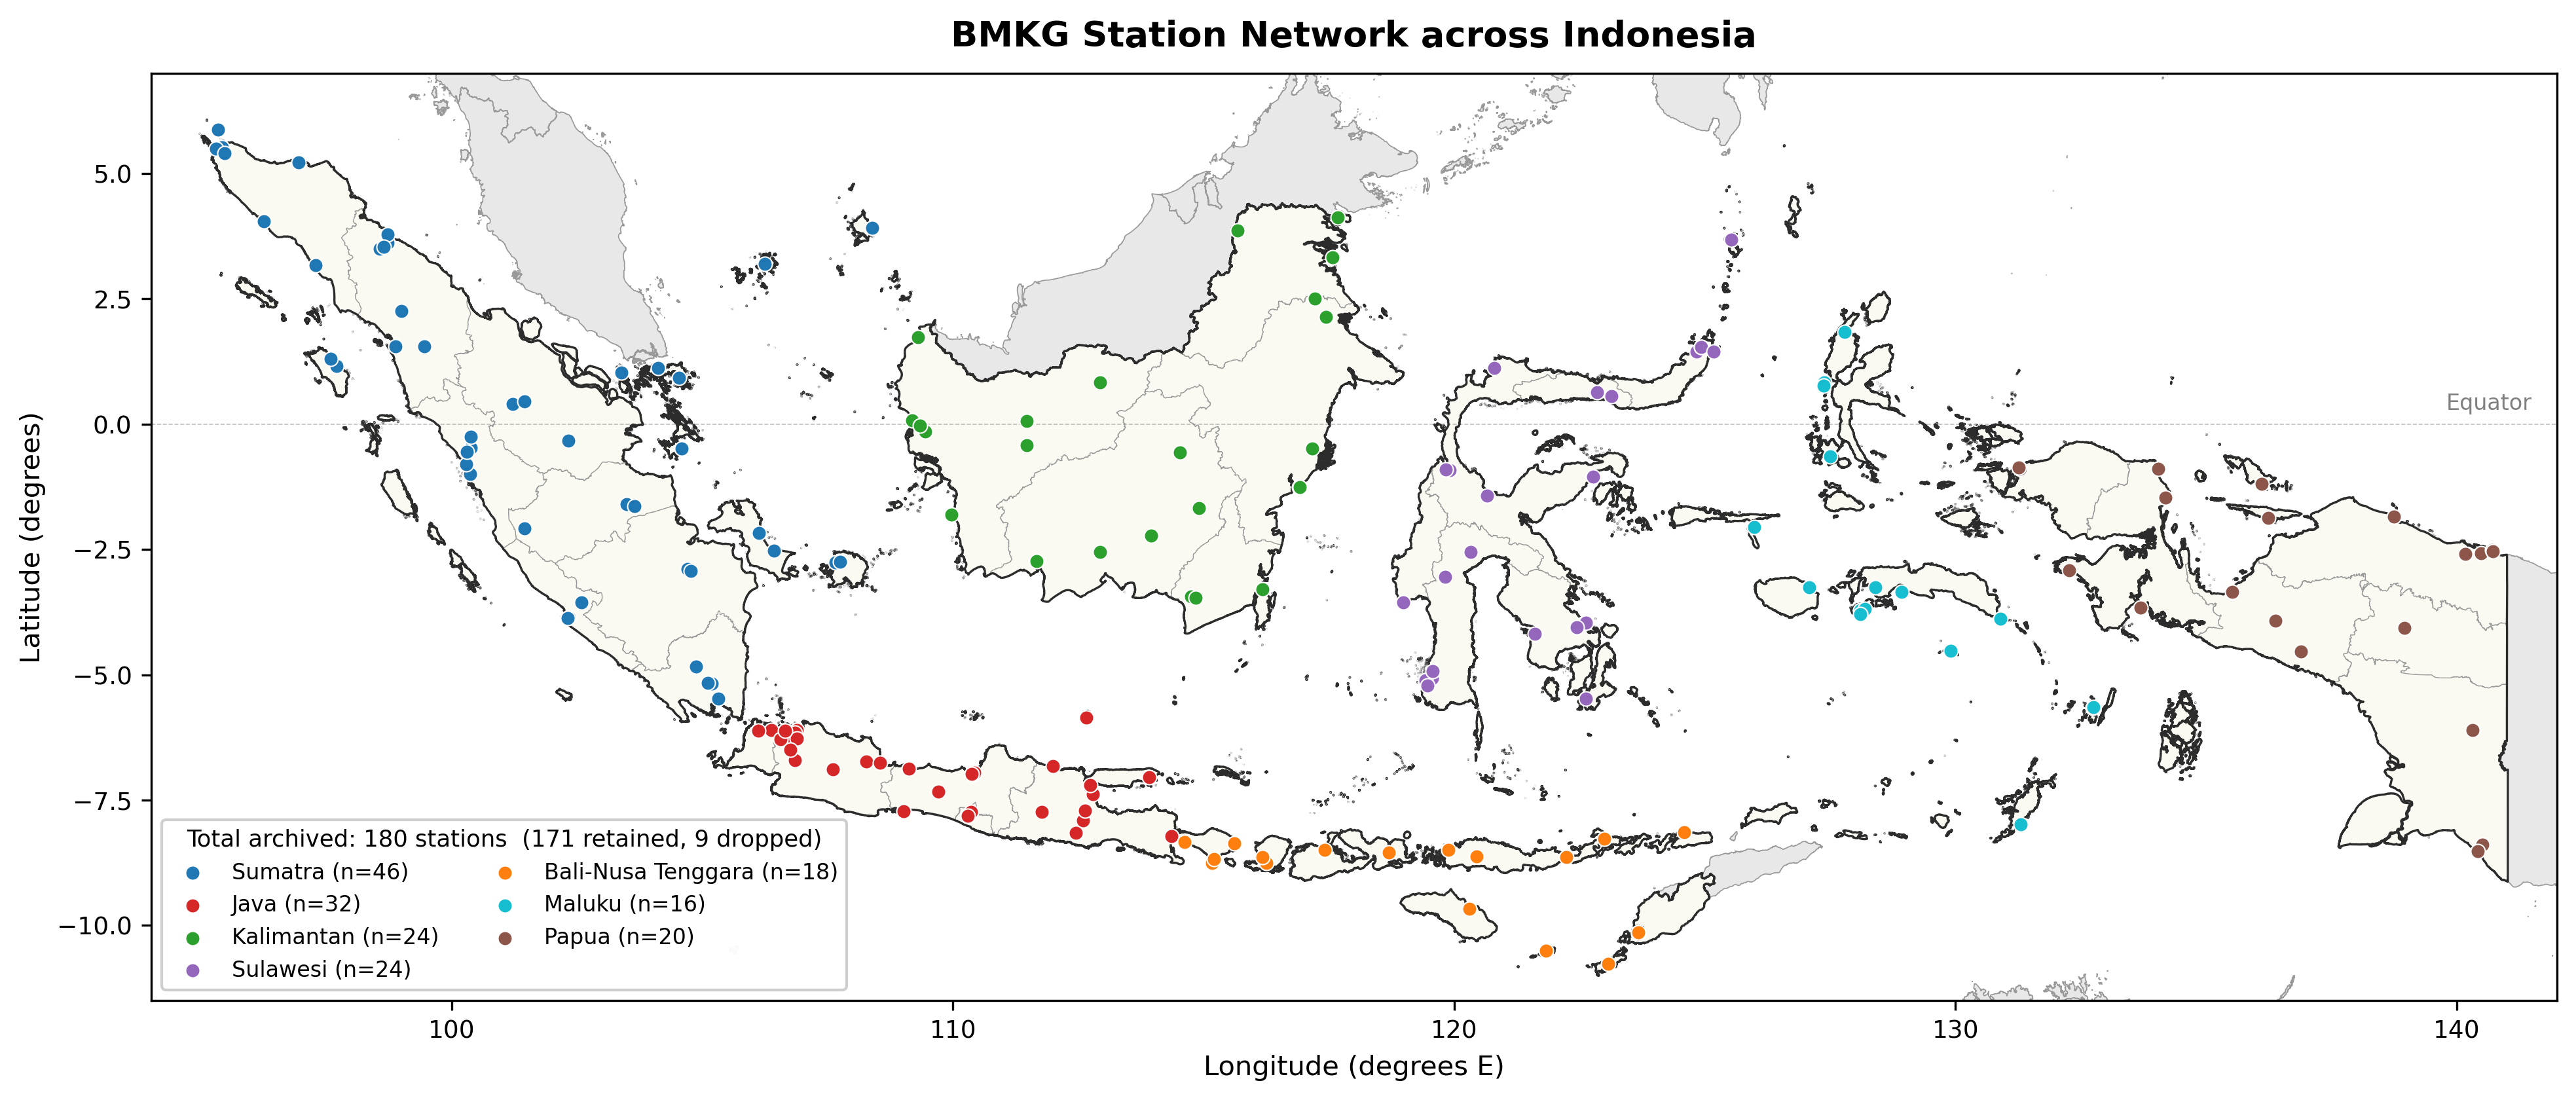
\includegraphics[width=\figThreeOneWidth\textwidth]{fig_thesis_03_station_map.png}
\caption[Spatial distribution of the 180 archived BMKG stations, color-coded by region]{Spatial distribution of the 180 archived BMKG stations, color-coded by region.\label{fig:station-map}}
\end{figure}


% ------------------------------------------------------------
\section{Four-Stage Hybrid Pipeline (LSEQM+DL)}\label{sec:methods-pipeline}
% ------------------------------------------------------------

The framework is built on a one-bias-dimension-per-stage design.
Section~\ref{sec:methods-data} described three bias modes that
IMERG-L carries against the gauge reference: a mean offset, a
distributional mismatch in the bulk, and a truncated upper tail.
Each of these has a matched correction stage: LS for the mean,
EQM with a Gamma fit for the bulk distribution, and GPD tail
adjustment for the extremes. A fourth stage, a CNN, addresses a
limitation that none of the marginal stages can reach by
themselves: the lack of spatial coherence in the extreme pixels
of a per-pixel statistical correction. The four stages execute
in sequence; the output of one stage becomes the input of the
next. All fitting is performed per pixel and per dekadal window,
with the 36 dekadal windows pooled across 2001 to 2025 giving
approximately 250 paired daily observations per pixel
per window. Figure~\ref{fig:pipeline} shows the conceptual
workflow, in which the final stage blends the CNN refinement with
the LSEQM result using a station-density-aware weight
(Section~\ref{sec:methods-blending}).

% Fig 3.2: dedicated page, image rotated 90 deg to occupy the page height
% as its new width (same approach as Fig 3.3 below). The PNG itself is the
% original landscape diagram; LaTeX handles the rotation.
\begin{figure}[p]
\centering
\rotatebox{90}{%
  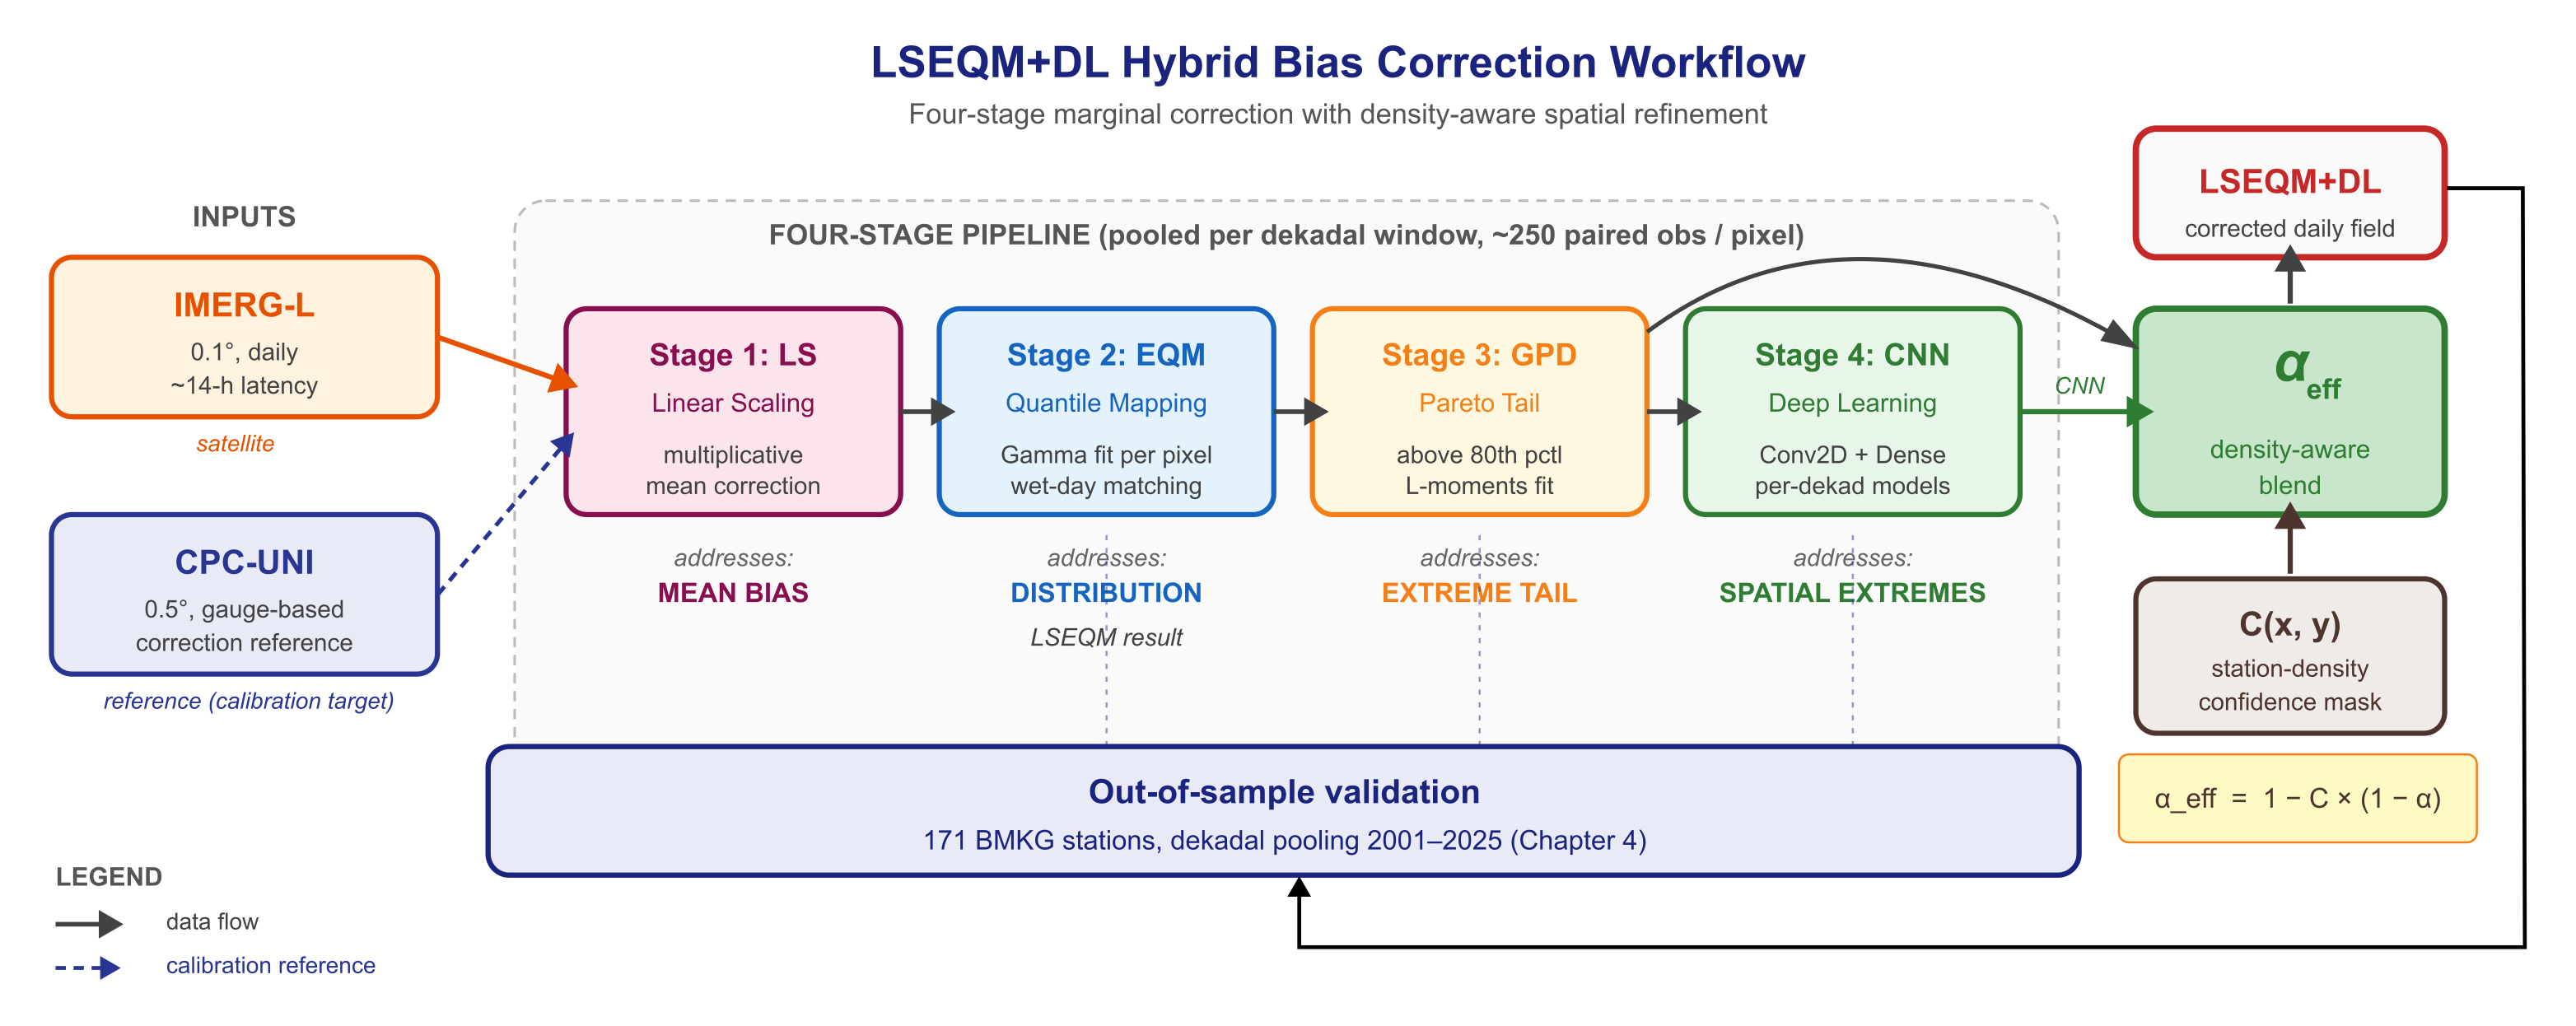
\includegraphics[width=\figThreeTwoWidth\textheight]{fig_thesis_03_pipeline.png}%
}
\caption[Conceptual workflow of the LSEQM+DL hybrid bias correction framework]{Conceptual workflow of the LSEQM+DL hybrid bias correction framework.\label{fig:pipeline}}
\end{figure}


\subsection{Mean Bias Correction: Linear Scaling}\label{sec:methods-ls}

The first stage addresses the mean offset between the satellite
and the gauge reference. For each CPC 0.5$^{\circ}$ cell~$c$ and
each dekadal window, a multiplicative correction factor is
computed from the pooled means of the satellite and reference
samples \citep{ref:teutschbein2012}:
\begin{equation}
P_{\text{LS}}(x, y, t) =
P_{\text{IMERG}}(x, y, t)
\cdot \frac{\overline{P}_{\text{CPC}}(c)}{\overline{P}_{\text{IMERG}}(c)},
\label{eq:ls}
\end{equation}
where $\overline{P}_{\text{CPC}}$ and $\overline{P}_{\text{IMERG}}$
are the pooled-dekad means of the gauge and satellite precipitation
within cell~$c$, respectively. The factor is applied to every
0.1$^{\circ}$ pixel that falls inside cell~$c$, following the
Bias Correction Spatial Disaggregation (BCSD) strategy of
\citep{ref:wood2004}. LS corrects the dekadal mean by construction;
it does not change the rank ordering of values within a pixel,
nor does it touch the distribution shape or the tail. Subsequent
stages address these remaining bias dimensions on the LS-corrected
series.


\subsection{Distribution Alignment: Empirical Quantile Mapping with Gamma}\label{sec:methods-eqm}

The second stage aligns the full marginal distribution of the
LS-corrected satellite series to the gauge reference. A
two-parameter Gamma distribution is fitted by maximum likelihood
to the wet-day subset of each pixel and each dekadal window,
yielding Gamma cumulative distribution functions (CDFs)
$F_{\text{IMERG},\Gamma}$ and $F_{\text{CPC},\Gamma}$
\citep{ref:gudmundsson2012, ref:themessl2012}. The corrected
value at day~$t$ is then obtained by quantile composition:
\begin{equation}
P_{\text{EQM}}(x, y, t) =
F_{\text{CPC},\Gamma}^{-1}\!
\left(F_{\text{IMERG},\Gamma}\!\left(P_{\text{LS}}(x, y, t)\right)\right).
\label{eq:eqm}
\end{equation}
The Gamma family is the standard parametric model for
daily precipitation on wet days. Its two parameters describe the
shape and the scale of the bulk distribution, where most of the
sample mass concentrates.

Because the gauge reference is coarser than the satellite product,
the CPC parameters cannot be applied at the IMERG resolution
directly. CPC-UNI is native to a $0.5^{\circ}$ grid while IMERG-L is
$0.1^{\circ}$, so each CPC cell spans a $5 \times 5$ block of IMERG
pixels. Following the bias-correction and spatial-disaggregation
principle \citep{ref:wood2004}, the Gamma, GPD, and dry-day
parameters are fit once at the native $0.5^{\circ}$ resolution and
bilinearly interpolated to the $0.1^{\circ}$ grid, rather than
regridding the gauge field itself; each $0.1^{\circ}$ pixel is then
quantile-mapped against its own interpolated reference distribution.
This disaggregates the correction, not the data: the satellite
retains its $0.1^{\circ}$ spatial detail and day-to-day sequence,
while the bilinear interpolation of the parameters avoids the
block-boundary artefacts that nearest-neighbour replication of a
$0.5^{\circ}$ field would impose. Figure~\ref{fig:bcsd} illustrates
the disaggregation on the Bali subdomain: panel~(a) shows that one
$0.5^{\circ}$ CPC cell covers a $5 \times 5$ block of $0.1^{\circ}$
pixels, panel~(b) the wet-day-mean parameter field fit at the native
$0.5^{\circ}$ resolution, panel~(c) the same field after bilinear
interpolation to $0.1^{\circ}$, and panel~(d) the per-pixel quantile
mapping of one $0.1^{\circ}$ pixel against its interpolated CPC
distribution.

\begin{figure}[H]
\centering
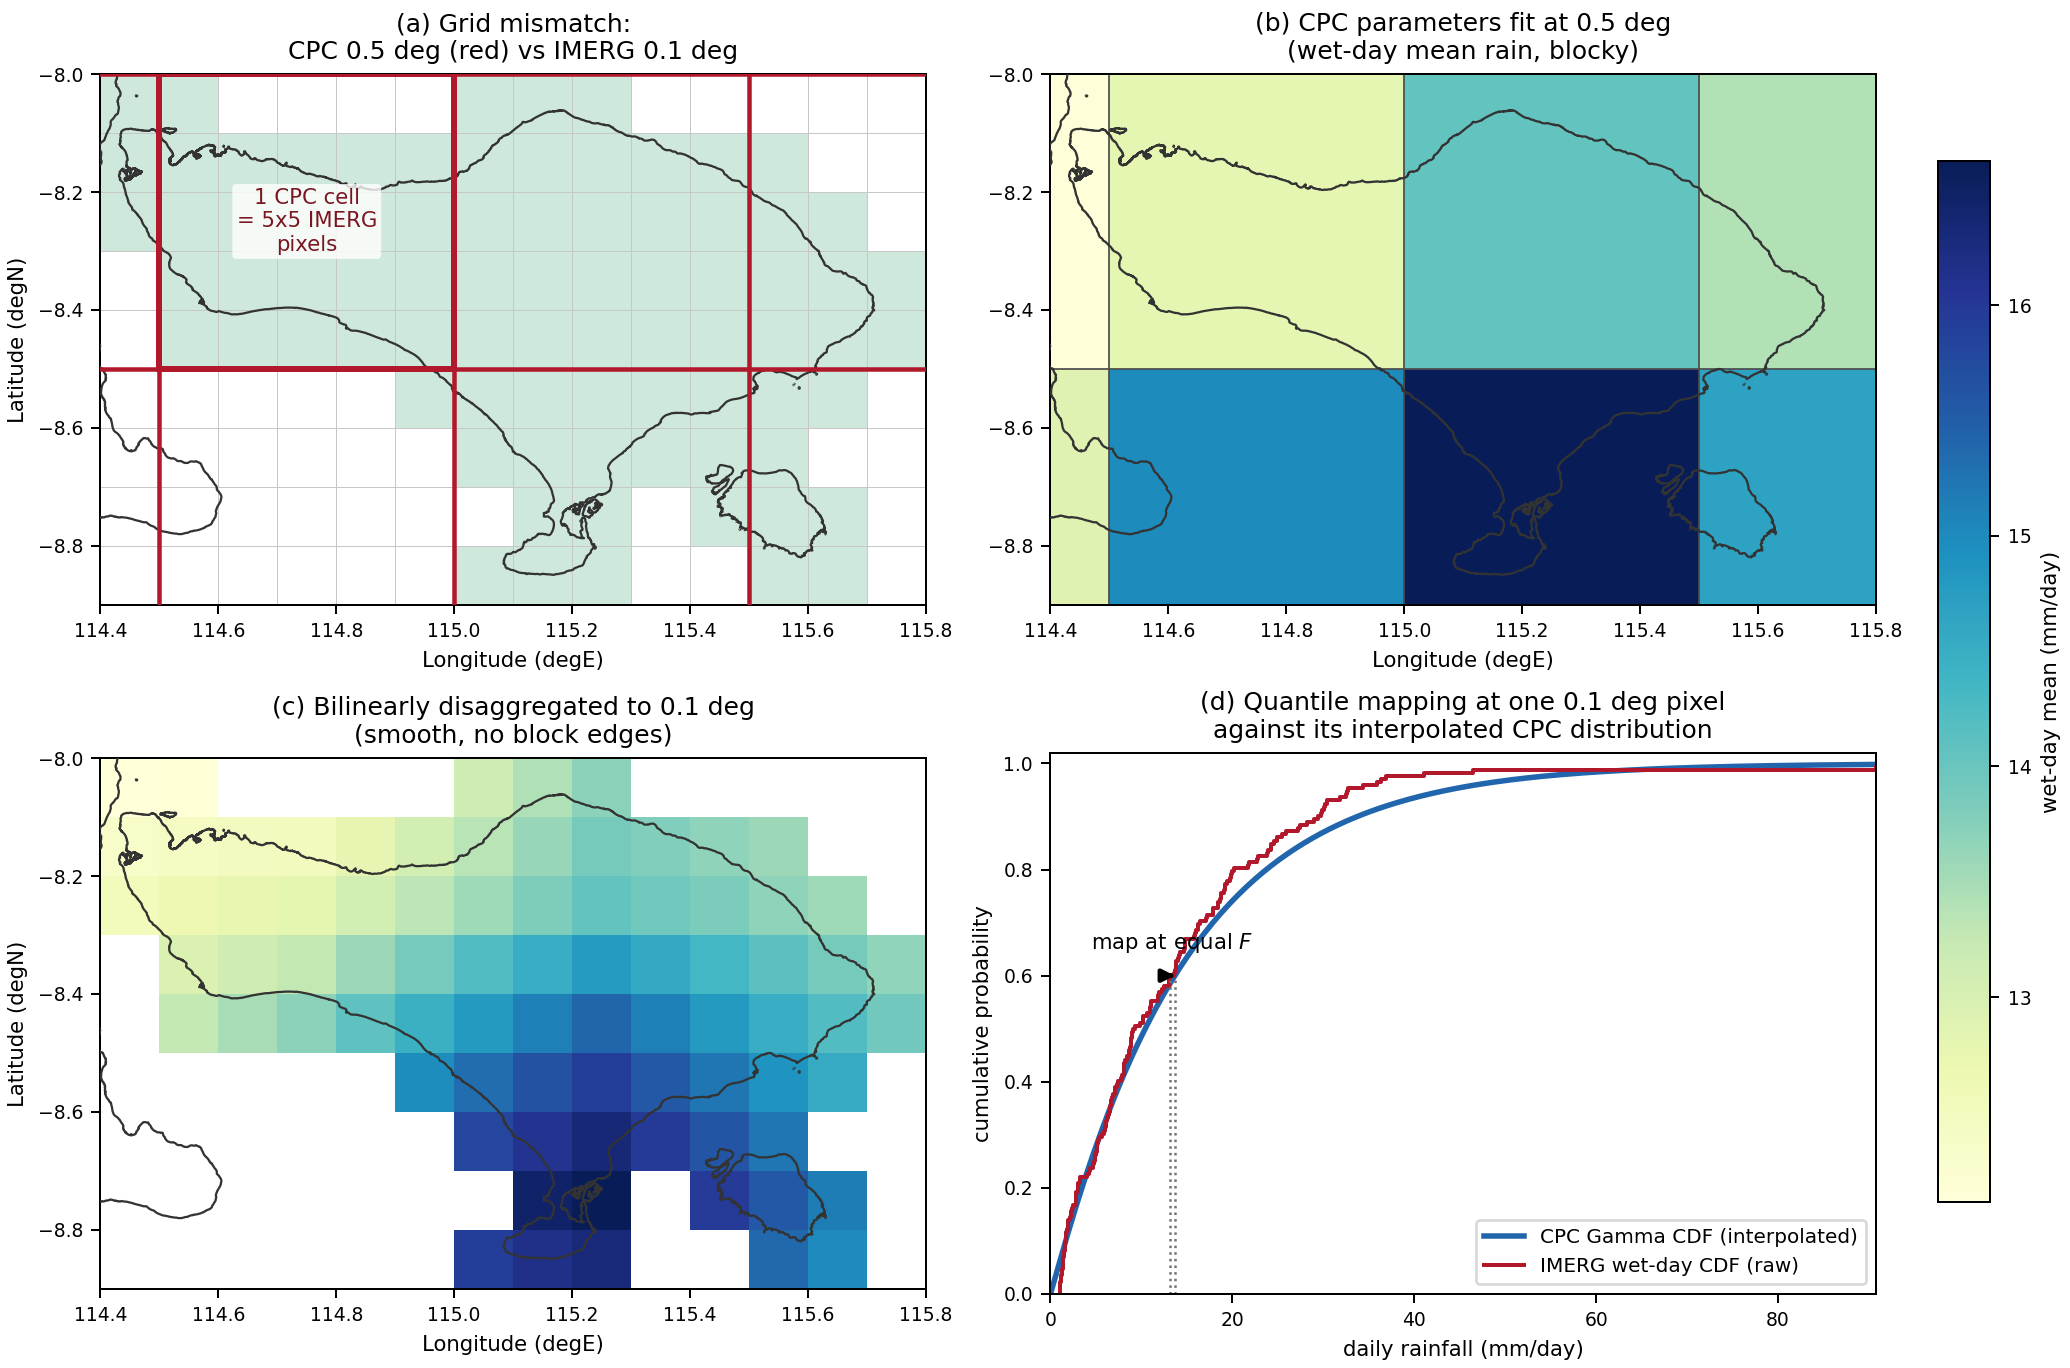
\includegraphics[width=\textwidth]{fig_thesis_03_bcsd_disaggregation.png}
\caption[Bias-correction spatial disaggregation of the CPC reference parameters from 0.5 to 0.1 degree]{Bias-correction spatial disaggregation of the CPC reference parameters from $0.5^{\circ}$ to $0.1^{\circ}$ on the Bali subdomain.\label{fig:bcsd}}
\end{figure}

Dry-day handling uses wet-day-frequency matching
\citep{ref:cannon2015}: the corrected series is constrained to
reproduce the gauge wet-day fraction within each dekadal window.
Days with $P_{\text{LS}} = 0$ are kept dry; days with non-zero
LS values that fall below the gauge wet-day threshold are
reclassified to dry. This mechanism is the source of the
event-detection trade-off discussed in
Chapter~\ref{chap:results}: matching the dry-day frequency
suppresses spurious light-rain events at the cost of reduced
aggregate probability of detection, but with the benefit of a
reduced false alarm ratio.

The Gamma family fits the bulk of the wet-day sample by design,
which means its parameters are dominated by light and moderate
rainfall, the segment that contains most of the sample mass. The
upper tail, the segment that is operationally meaningful for
flood and drought thresholds, is fit only as a by-product and is
systematically too short. The next stage corrects this.


\subsection{Extreme Tail Preservation: Generalized Pareto Distribution}\label{sec:methods-gpd}

\medskip\noindent\textbf{Motivation.}
The Gamma fit in Stage~2 is a two-parameter distribution fitted
to the full wet-day sample. By construction its parameters are
dominated by the bulk of the sample, that is, the light to
moderate rainfall that contains most of the points. The upper
tail, which is the segment operationally meaningful for flood
and drought thresholds, is fit only as a by-product of forcing
the Gamma curve through the bulk, and for tropical precipitation
is systematically too short. Gamma cannot represent the heavy
tail that real tropical convective rainfall exhibits. Stage~3
grafts a GPD onto the upper
tail, fitted explicitly to exceedances above a high threshold.
The GPD is the canonical extreme-value model in the
peaks-over-threshold framework: under mild regularity conditions
the distribution of exceedances above a high threshold converges
to a GPD with shape and scale parameters $(\xi, \sigma)$
\citep{ref:coles2001}, with cumulative distribution function
\begin{equation}
F_{\text{GPD}}(x; u, \sigma, \xi) =
1 - \left[1 + \xi\,\frac{x - u}{\sigma}\right]^{-1/\xi},
\quad x > u,
\label{eq:gpd}
\end{equation}
where $u$ is the threshold. The shape parameter $\xi$ controls
tail heaviness: $\xi > 0$ indicates a heavy Pareto-like tail
typical of tropical convective extremes, $\xi = 0$ an exponential
tail, and $\xi < 0$ a bounded tail.

\medskip\noindent\textbf{Method.}
For each pixel and each dekadal window, the GPD fit proceeds in
seven steps.

\begin{enumerate}
    \item Extract the wet-day subset of the 25-year sample
    (approximately 250 paired days multiplied by the wet-day fraction).
    \item Reuse the Gamma fit from Stage~2 as the bulk model.
    \item Compute the 80th-percentile threshold of the wet
    sample.
    \item Extract exceedances (wet observations above the
    threshold), typically 50 points if the wet sample has 250
    entries (250 times 0.20).
    \item Fit GPD parameters $(\xi, \sigma)$ to the exceedances
    by maximum likelihood with the location parameter fixed at
    the threshold \citep{ref:coles2001}; the parameters are
    averaged across five subsamples to reduce variance on the
    small per-pixel exceedance set (see
    Section~\ref{sec:methods-gpd} subsection on subsample
    aggregation below).
    \item Above the 80th percentile, replace the Gamma-based
    quantile from Stage~2 with the GPD-based quantile.
    \item Cap the final value at the 99.9th percentile of the
    CPC reference distribution as a safety net against GPD
    over-extrapolation in the extreme tail.
\end{enumerate}

The replacement in step~6 is a quantile remap through the
reference tail. For a satellite value $P_{\text{LS}}$ above the
satellite threshold $u_{\text{sat}}$, the conditional exceedance
probability within the satellite tail is
\begin{equation}
p_c = \frac{F_{\text{sat}}(P_{\text{LS}}) - F_{\text{sat}}(u_{\text{sat}})}
           {1 - F_{\text{sat}}(u_{\text{sat}})},
\label{eq:gpd-pc}
\end{equation}
where $F_{\text{sat}}$ is the satellite wet-day cumulative
distribution. This probability is then mapped onto the reference
tail through the inverse of the reference GPD cumulative
distribution $G_{\text{ref}}$, anchored at the reference
threshold $u_{\text{ref}}$:
\begin{equation}
P_{\text{LSEQM}} = u_{\text{ref}} + G_{\text{ref}}^{-1}(p_c).
\label{eq:gpd-map}
\end{equation}
In the implementation the reference GPD is fitted to the
threshold exceedances $x - u_{\text{ref}}$ with its location
pinned to zero, so $G_{\text{ref}}^{-1}(p_c)$ returns an
exceedance above $u_{\text{ref}}$ and the threshold is added
back to recover the absolute value.
Equations~\eqref{eq:gpd-pc} and~\eqref{eq:gpd-map} preserve the
rank of the satellite value within its own tail and place it at
the matching quantile of the reference tail, so the heavy-tail
shape of the corrected field follows the reference GPD rather
than the truncated Gamma extrapolation of Stage~2.

\medskip\noindent\textbf{Threshold choice and sample-size considerations.}
The 80th-percentile threshold is unconventionally low for a GPD
fit. Standard practice in extreme-value analysis uses the 90th
to 99th wet-day percentile, justified per region by mean
residual life plots or parameter-stability diagnostics
\citep{ref:coles2001}. The present study made an empirical
trade-off in the other direction: a 90th-percentile choice would
yield only about 25 exceedances per pixel-dekad at the typical
wet-day fraction, on the edge of the sample size at which the
GPD Maximum Likelihood Estimation (MLE) becomes operationally noisy \citep{ref:hoskingwallis1987};
the 80th-percentile choice yields about 50 exceedances and
trades cleanliness of the extreme regime for sample-size
stability. Lower thresholds (60th or 70th) would yield still
more exceedances but conflate the extreme tail with moderate
rain that the Gamma EQM already represents adequately. The
threshold was not formally optimised nor diagnosed with the
standard residual-life plots; its empirical effect on the
headline metrics is reported in
Section~\ref{sec:results-sensitivity} and the limitation is
acknowledged in the chapter close.

The 80th-percentile choice carries a hidden assumption: every
pixel and dekad combination has enough wet days for stable GPD
fitting. Whether this holds depends on the local wet-day
fraction. To obtain about 30 exceedances at the 80th percentile,
a pixel needs about 150 wet days in the pooled 250-day sample
(since $30 / 0.20 = 150$). Wet-day fractions in Indonesia vary
dramatically with season and region: wet-season Java sees
approximately 70 to 80~percent wet days, giving 175 to 200 wet
days and 35 to 40 exceedances, a comfortable margin. Dry-season
eastern Nusa Tenggara sees approximately 10 to 20~percent wet
days, giving 25 to 50 wet days and only 5 to 10 exceedances,
well below the practical floor for a stable MLE.

In the latter case the GPD fit returns a degenerate default
(shape~$= 0$, location~$= 0$, scale~$= 1$) that produces the
trivial mapping $y = x$, effectively disabling the tail
adjustment for that pixel and leaving the Gamma EQM value in
place. The fallback is defensible in genuinely dry pixels, where
the few wet days are climatologically light-rain events and the
Gamma EQM result is the right answer by default; the fallback
is less defensible in pixels with 25 to 50 wet days, where heavy
events do exist but cannot be fit reliably. The fraction of
pixel-dekads in which the GPD adjustment is active versus
fallback was not reported as a spatial diagnostic in the present
study; producing such a map would be a useful supplementary
artefact for future work.

\medskip\noindent\textbf{Why subsample-averaged MLE rather than a single fit.}
A single GPD maximum-likelihood fit to approximately 50
exceedances has wide confidence intervals on both $\xi$ and
$\sigma$. The rule of thumb in \citep{ref:coles2001} is that GPD
parameter uncertainty becomes operationally tolerable around 100
or more exceedances; with 50 points the single-fit estimate is
noisy and sensitive to a small number of high-leverage values.
A subsample-averaging step reduces estimator variance: the
exceedances are partitioned into five folds of about 10 points
each, the GPD is fitted by maximum likelihood on four folds at a
time (40 points), the parameters $(\xi, \sigma)$ are recorded,
the partition rotates across all five subsamples, and the final
estimate is the mean of the five parameter pairs. The procedure
resembles the subsample step of a bootstrap and reduces variance
arising from a single high-leverage exceedance, but it is not
itself a cross-validation in the strict statistical sense (no
held-out evaluation is performed) and it does not eliminate the
small-sample bias of the GPD shape MLE \citep{ref:hoskingwallis1987}.
The trade is a deliberate one: at 40 to 60 exceedances the
shape estimator is biased but the bias is comparable in
magnitude across folds, so averaging suppresses noise without
making the bias worse.

\medskip\noindent\textbf{Implementation notes.}
The threshold is computed per pixel on the satellite distribution,
not domain-wide and not on the reference. Each pixel uses its
own 80th percentile of its own wet sample. A pixel in Java
might have a threshold around 25~mm/day; a pixel in eastern
Nusa Tenggara might have a threshold of about 8~mm/day. This
per-pixel behaviour is the correct response to the
climatological heterogeneity of the domain. Below the threshold
the Gamma EQM result is used; above it, the GPD-adjusted
quantile is used. There is no smoothing across the join: the
two curves are constrained to match at the threshold percentile,
so the discontinuity is small in practice but is not exactly
zero. The 99.9th-percentile cap is also computed per pixel and
varies spatially: over wet-season Java the cap is on the order
of 200 to 400~mm/day, while over dry-season eastern Nusa
Tenggara it may be 50 to 80~mm/day.


\subsection{Spatial Refinement of Extremes: Convolutional Neural Network}\label{sec:methods-cnn}

The first three stages each operate one pixel at a time. After
the GPD step the corrected field has the right marginal
distribution at every pixel, with the mean from LS, the bulk
shape from Gamma EQM, and the tail from GPD. What it still lacks
is spatial coherence among the extreme pixels. A 100~mm event in
a cluster of adjacent pixels reflects organised convection and
is climatologically plausible; a 100~mm event in a single pixel
surrounded by 5~mm pixels is more likely a satellite retrieval
artefact. Per-pixel statistical correction cannot tell the two
apart, because each pixel is corrected independently.

The fourth stage is a small CNN
that refines extreme-pixel values using local spatial context.
The architecture, implemented in \texttt{src/deep\_learning.py},
is a sequential stack of two Conv2D layers (each followed by
MaxPool2D and Dropout), a Flatten layer, a 128-unit Dense
bottleneck (followed by a third Dropout), and a final Dense
output layer that reconstructs the full grid
\citep{ref:pan2019, ref:banomedina2020}. The output layer uses a
\textit{linear} activation rather than ReLU or sigmoid;
precipitation is non-negative, but a ReLU at the output would
clamp at zero and remove the gradient signal that the mean
squared error loss needs to refine values near the threshold.
The non-negativity constraint is enforced by clipping the
blended output at zero in post-processing; the
99.9th-percentile cap from Section~\ref{sec:methods-gpd} bounds
the upper tail separately and is not re-applied after blending.
Dropout in three places (after each of the two MaxPool layers
and after the Dense bottleneck) provides aggressive
regularisation. The final Dense layer reconstructs the full
grid and dominates the parameter count, so the network is large
relative to the per-dekad training sample; the risk of
overfitting is contained at inference rather than by the
architecture, through applying the refinement only to extreme
pixels, capping its contribution through the blend weight, and
disabling it where station density is low, as discussed below. A
fully-convolutional reconstruction head, prototyped on the Bali
subdomain, matches the dense model's station-validation skill
while cutting the Stage-4 parameter count by roughly $900$ times
at the full Indonesia resolution; the dense head is retained here
so that the released models reproduce the numbers reported in this
thesis, with the fully-convolutional variant available through the
\texttt{architecture} option as the recommended extension for
full-resolution deployment.

The model is trained one per dekadal window on the LSEQM-corrected
field as input and the CPC-UNI reference as target. Loss is
mean squared error over the full field; the extreme-pixel
restriction is applied only at the blending step, not during
training. The Adam
optimizer \citep{ref:kingma2014} drives the parameter update,
and an internal $80/20$ train-validation split with early
stopping (patience of five epochs) controls the number of
training epochs. Thirty-six independent models are produced
and saved for inference. The per-dekad training sample is
approximately 200 days for training and 50 days for validation
after the split. The split is implemented as a random
within-dekad partition rather than a strict temporal hold-out,
so the train and validation samples are drawn from the same
2001 to 2025 range; this is a deliberate compromise that
preserves sample size at the cost of not testing
out-of-distribution generalisation strictly. The batch size
is auto-shrunk at training time if the configured value would
require more than approximately 2~GB per batch on the
$171 \times 461$ Indonesian grid, which it typically does at
default settings.

Three properties of the design constrain the role of the CNN.
First, it operates only above the GPD threshold; sub-threshold
pixels pass through the LSEQM result unchanged. Second, its
output is blended with the LSEQM result rather than replacing
it, under a default weight $\alpha = 0.70$ for LSEQM and
$1 - \alpha = 0.30$ for CNN. Third, the blending weight is
modulated by a station-density confidence mask described in
Section~\ref{sec:methods-blending}, so that the CNN contribution
is suppressed in regions where the CPC reference itself is
weakly constrained by the contributing gauge network. These
three constraints together mean the CNN refines rather than
replaces the statistical baseline: it cannot undo the work of
the earlier stages, and the framework reduces cleanly to LSEQM
when the blend weight is set to $\alpha = 1$, which is the
ablation row reported in the sensitivity analysis of
Section~\ref{sec:results-sensitivity}. The blend weight
$\alpha = 0.70$ and the dependence on station density are
design choices that were not formally optimized; their
sensitivity is reported in
Section~\ref{sec:results-sensitivity}.

Three implementation quirks are worth flagging for any reader
who plans to extend or reuse the CNN component. First, the
choice of mean squared error rather than mean absolute error
penalises large deviations more heavily, which is the right
loss when the goal is to fit the upper tail of the
precipitation distribution; a defensible alternative would be
a quantile loss focused on the same tail, but this was not
tried. Second, the saved model expects a fixed input shape
matching the $171 \times 461$ Indonesian grid; transferring
the framework to a different domain or grid resolution
requires retraining rather than direct inference. Third, a
spatial diagnostic of per-dekad CNN validation loss across the
36 dekadal windows would surface seasons in which the CNN
contribution is weaker because the training extreme-event
sample is thinner (typically dry-season dekads with few
heavy-rain events); such a diagnostic is not formally produced
in the present study and is flagged in
Section~\ref{sec:methods-cnn} as a useful supplementary
artefact for future work.

Figure~\ref{fig:cnn-arch} shows the CNN architecture in detail
alongside the station-density-aware blending mechanism that
Section~\ref{sec:methods-blending} formalises.

% Fig 3.3: dedicated page, image rotated 90 deg to occupy the page height
% as its new width. The original PNG is landscape-oriented; rotating it
% lets the reader see the full diagram at print scale without reducing it
% to thumbnail size on the body text width.
\begin{figure}[p]
\centering
\rotatebox{90}{%
  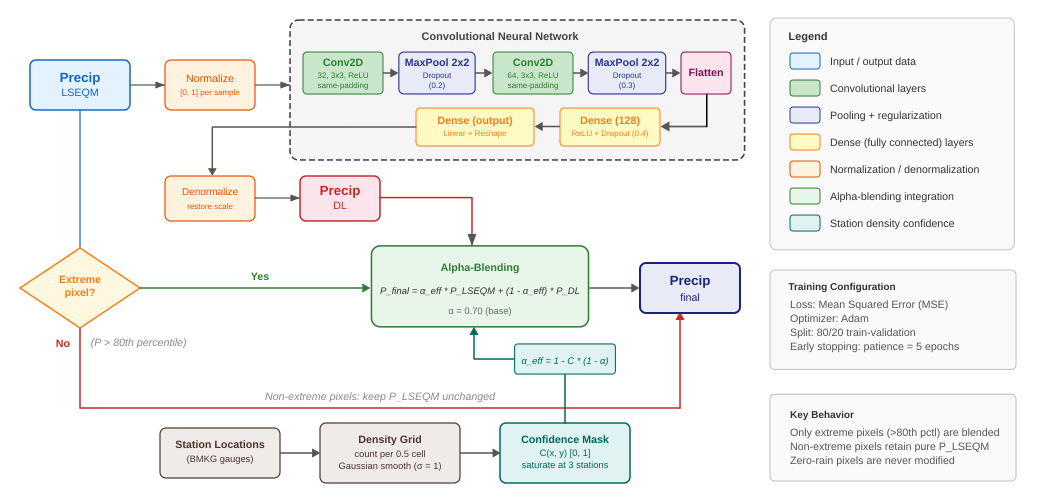
\includegraphics[width=\figThreeThreeWidth\textheight]{fig_thesis_03_cnn_workflow.png}%
}
\caption[Stage~4 architecture: CNN forward pass, alpha-blending, and station-density confidence mask]{Stage~4 architecture in detail: the Convolutional Neural Network forward pass, the alpha-blending step that combines the CNN refinement with the LSEQM intermediate, and the station-density confidence-mask construction.\label{fig:cnn-arch}}
\end{figure}
\clearpage

Figure~\ref{fig:stage-demo} shows the effect of the four stages
on an illustrative 60-day sample, arranged in a $5 \times 2$
grid read from top to bottom. The reference shown in the figure
is the CPC-UNI calibration target the pipeline acts on; the
independent out-of-sample validation against 172 BMKG stations
is reported in Chapter~\ref{chap:results}. Panels (a, b) show the
raw input and the LS mean match; panels (c, d) show the EQM
quantile-mapping mechanism and its effect on the daily series;
panels (e, f) show the GPD adjustment on the series and on the
wet-day tail; panels (g, h) show the CNN refinement and the final
corrected output; and panels (i, j) summarise the cross-stage
distributions and the headline metrics. The data are synthetic for
illustration; the empirical numbers for the BMKG validation
appear in Chapter~\ref{chap:results}.

Read together, the panels make the division of labour between the
stages concrete. The LS step in panel (b) lifts the whole series
to the gauge mean but leaves the day-to-day spread too narrow, so
the heaviest days stay under-corrected. The EQM step in panels
(c, d) widens the wet-day distribution to match the gauge, yet a
Gamma fit alone still clips the rarest events. The GPD step in
panels (e, f) restores those upper-tail days without disturbing the
bulk of the distribution, and the CNN refinement in panel (g) moves
only the extreme pixels toward the reference. The cumulative effect
in panel (h) is a series whose mean, spread, and tail all track
CPC-UNI; the empirical distributions in panel (i) and the metric
summary in panel (j) confirm that relative bias, the
standard-deviation ratio, and the 99th-percentile ratio each move
toward their targets across the four stages.

\begin{figure}[H]
\centering
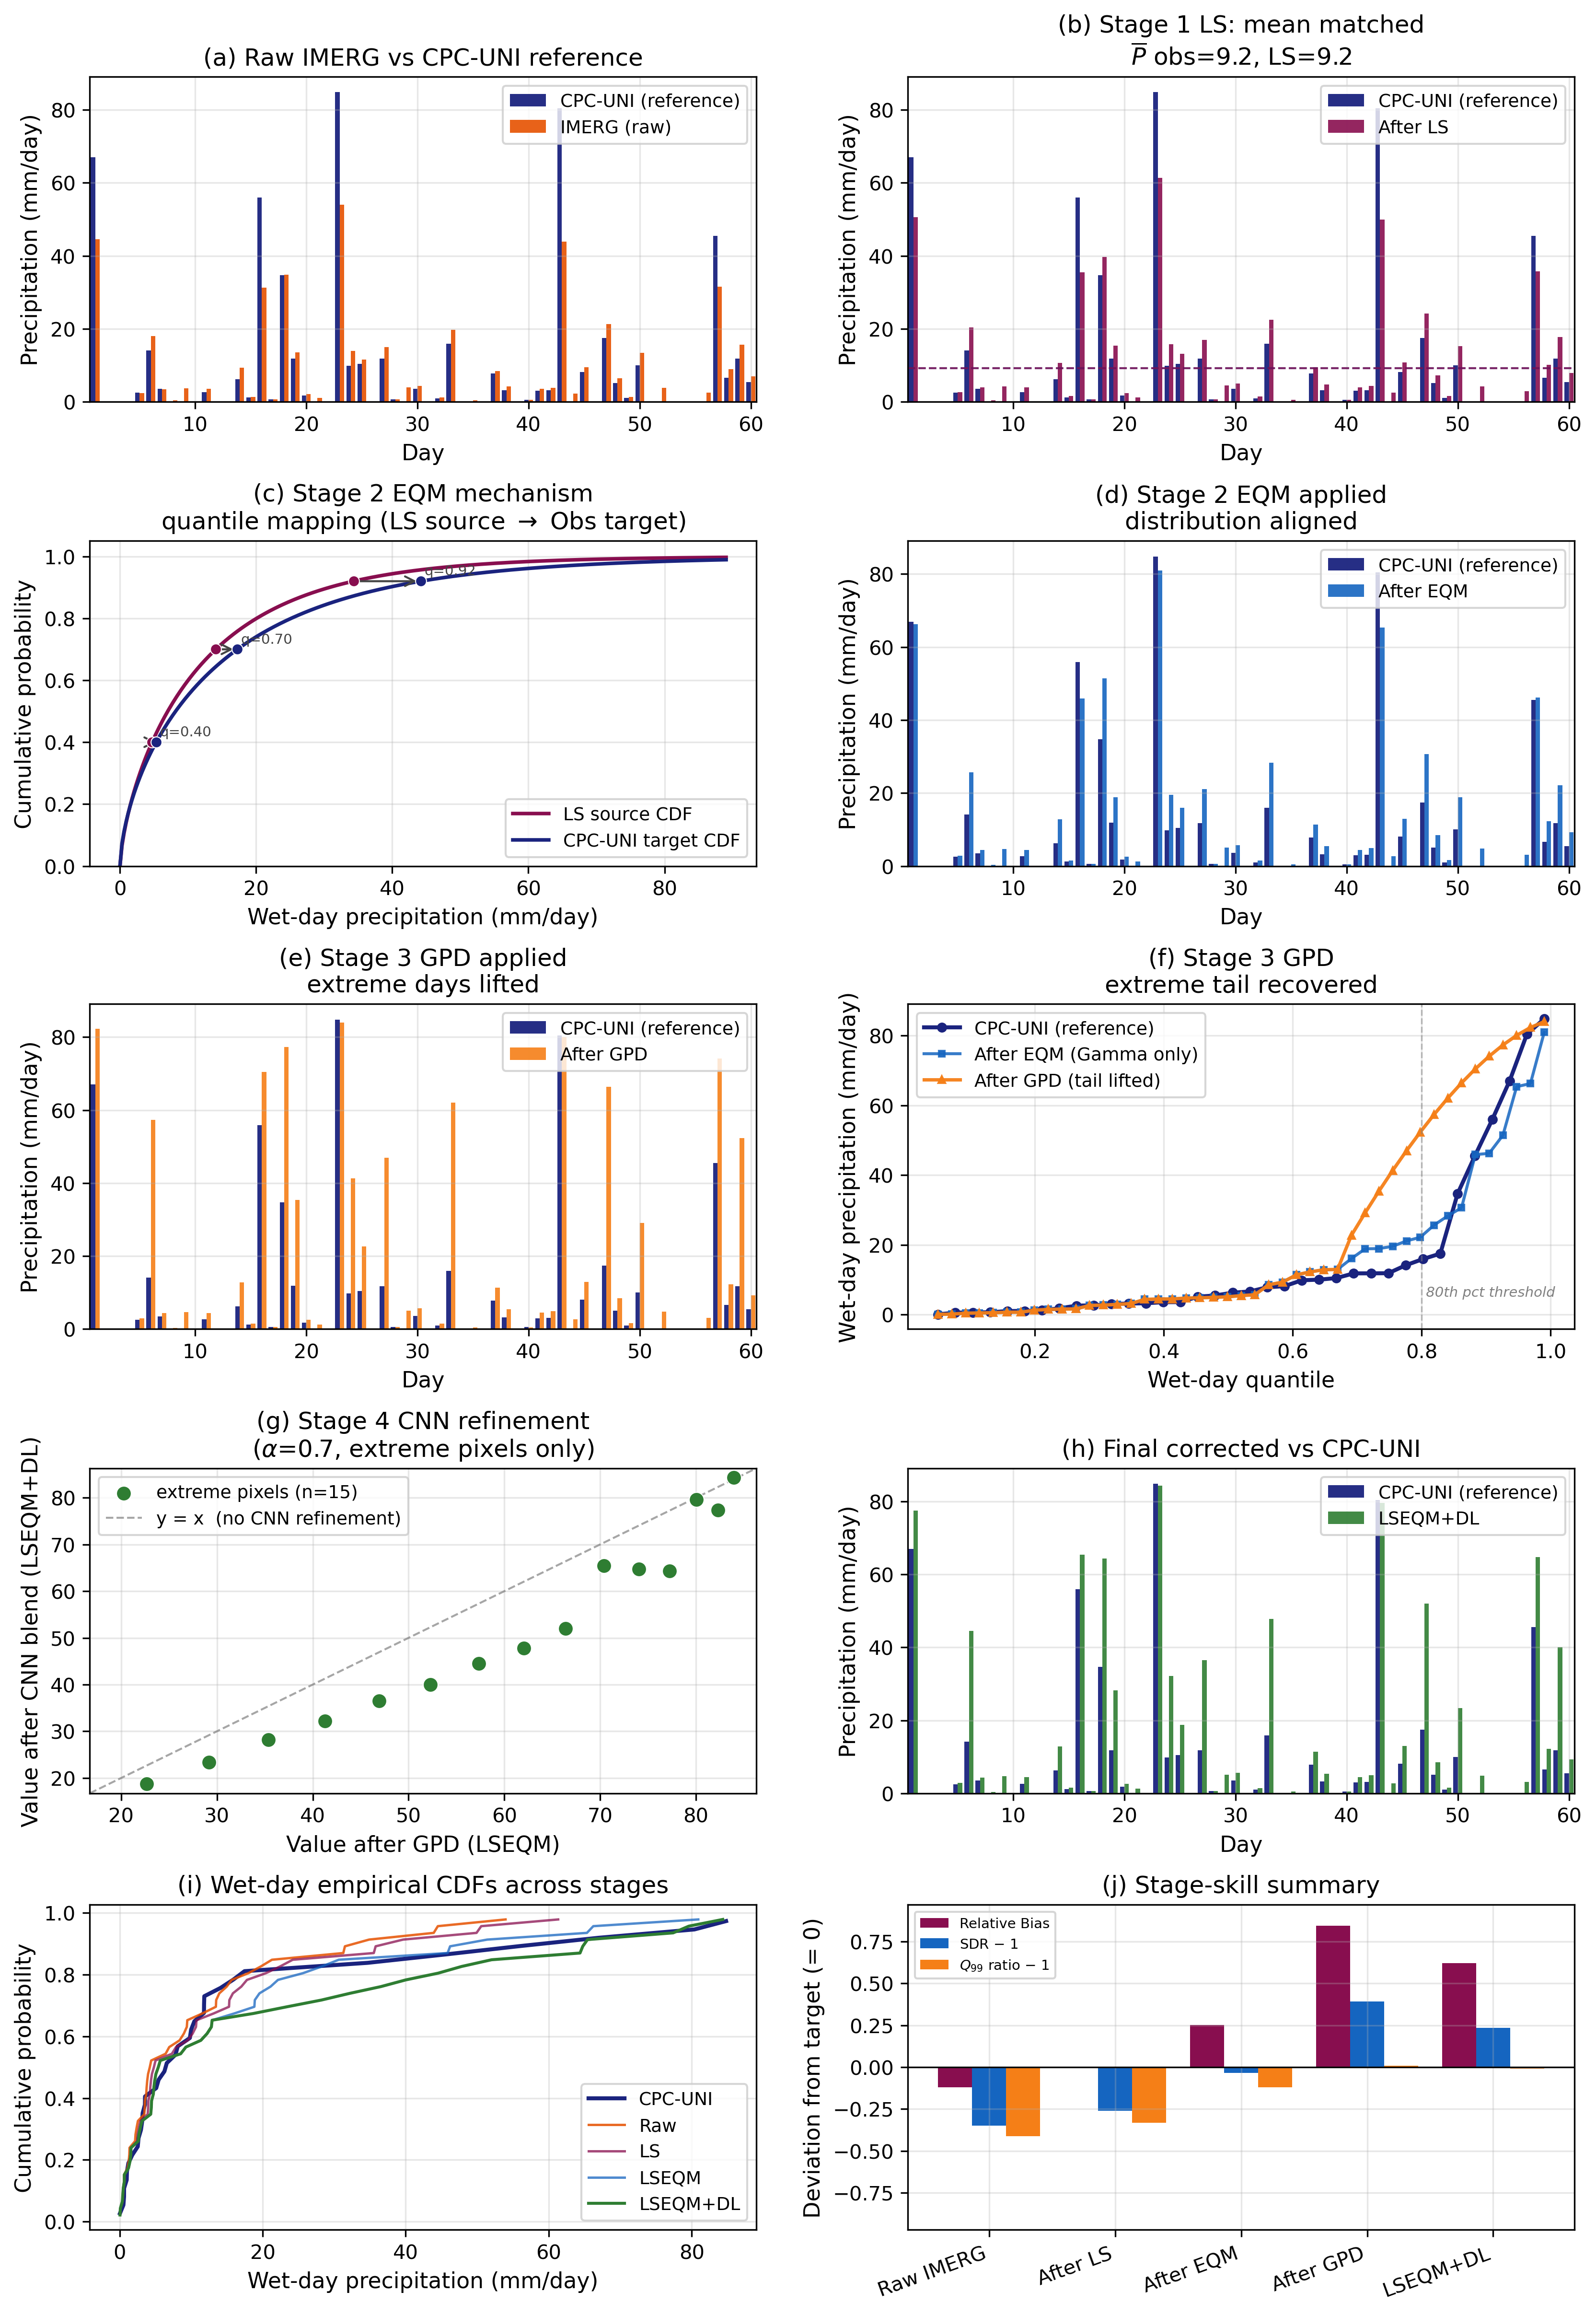
\includegraphics[width=\figThreeFourWidth\textwidth]{fig_thesis_03_stage_demonstration.png}
\caption[Illustrative effect of the LSEQM+DL pipeline stages applied to a synthetic 60-day daily-precipitation sample]{Illustrative effect of the LSEQM+DL pipeline stages applied to a synthetic 60-day daily-precipitation sample.\label{fig:stage-demo}}
\end{figure}


% ------------------------------------------------------------
\section{Station-Density-Aware Blending}\label{sec:methods-blending}
% ------------------------------------------------------------

The CNN refinement in Stage~4 is trained against CPC-UNI, and
the quality of CPC-UNI itself depends on the local density of
contributing gauges. Over Java and southern Sumatra the
contributing network is dense and CPC-UNI is a well-constrained
reference. Over Papua, Maluku, and eastern Nusa Tenggara the
network is sparse and CPC-UNI is essentially a smooth-field
reconstruction from few stations. Training a CNN to refine
extremes against such a reference, and then applying the CNN at
its nominal weight everywhere, would let reference uncertainty
in sparse regions propagate into the corrected product. The
blending stage addresses this by making the CNN-versus-LSEQM
weight depend on local gauge density rather than on a constant.
This is a design choice introduced to make the framework
deployable beyond Java without per-region hand-tuning, and is
not claimed as a key contribution of the present work.

Let $C(x, y) \in [0, 1]$ denote a station-density confidence
field constructed once for the domain and cached. The final
corrected value at every pixel above the GPD threshold is the
density-weighted blend of the LSEQM result and the CNN refinement:
\begin{equation}
P_{\text{final}}(x, y, t) =
\alpha_{\text{eff}}(x, y) \cdot P_{\text{LSEQM}}(x, y, t)
+ (1 - \alpha_{\text{eff}}(x, y)) \cdot P_{\text{CNN}}(x, y, t),
\label{eq:blend}
\end{equation}
where the effective blend weight $\alpha_{\text{eff}}$ modulates
the nominal value $\alpha = 0.70$ by the confidence field:
\begin{equation}
\alpha_{\text{eff}}(x, y) = 1 - C(x, y) \cdot (1 - \alpha).
\label{eq:alpha-eff}
\end{equation}
Equation~\ref{eq:alpha-eff} has the following behaviour across
the confidence range:
\begin{itemize}
    \item $C = 1$ gives $\alpha_{\text{eff}} = 0.70$, the
    nominal $30\%$ CNN contribution where the reference is
    well-constrained by the contributing gauge network.
    \item $C = 0.5$ gives $\alpha_{\text{eff}} = 0.85$, a
    $15\%$ CNN contribution at intermediate gauge density.
    \item $C = 0$ gives $\alpha_{\text{eff}} = 1.00$, pure
    LSEQM with the CNN fully suppressed where the reference is
    weak.
\end{itemize}
The relationship between confidence and effective weight is
linear and continuous across this range. The blend is applied
only to pixels above the GPD threshold from
Section~\ref{sec:methods-gpd}; sub-threshold pixels pass
through the LSEQM result unchanged.

The confidence field $C(x, y)$ is built in three steps. First,
the BMKG gauge-station locations of
Section~\ref{sec:methods-data} are counted within each
$0.5^{\circ}$ CPC cell as a proxy for how densely the reference
is constrained there. The same station archive supplies the
out-of-sample validation points, so the deep-learning
refinement is most active in the cells where validation stations
are densest; because the refinement is capped and acts only on
extreme pixels, gauge values are not transferred into the
validation comparison, but this coupling between the density
gate and the validation network is noted here.
Second, the count field is smoothed with
a Gaussian filter of standard deviation $\sigma = 1$ cell, which
corresponds to an e-folding distance of approximately 55~km at
0.5$^{\circ}$ resolution. The smoothing scale is matched to the
CPC-UNI interpolation scale so that the confidence field is
defined at the spatial frequency at which the reference itself
is resolved. Third, the smoothed count is divided by a
saturation parameter and clipped to the unit interval:
\begin{equation}
C(x, y) = \min\!\left(
\frac{(\text{count} \ast G_{\sigma=1})(x, y)}{c_{\text{sat}}},
\; 1
\right),
\label{eq:confidence}
\end{equation}
where $G_{\sigma=1}$ is the Gaussian smoothing kernel and
$c_{\text{sat}} = 2$ is the saturation parameter used in the
present study. The confidence field is then bilinearly
interpolated from the 0.5$^{\circ}$ CPC grid to the
0.1$^{\circ}$ IMERG grid, matching the BCSD strategy applied
elsewhere in the pipeline. The field is computed once, cached as
a NetCDF artefact at \texttt{data/output/station\_density/}, and
reused for every dekadal window and every method.

Both the nominal blend weight $\alpha = 0.70$ and the saturation
parameter $c_{\text{sat}} = 2$ are sensitivity parameters that
were not formally optimized. An earlier configuration of the
pipeline used $c_{\text{sat}} = 3$; qualitative inspection of
the resulting CNN-active fraction across the domain showed that
the higher value suppressed CNN refinement almost everywhere
outside Java and removed the contribution the CNN was designed
to provide, and the default was therefore reduced to 2 for the
present study. The other endpoint is similarly avoided: a lower
parameter (such as $c_{\text{sat}} = 1$) would extend CNN
influence into regions where the CPC reference is too sparse to
support training, which is the failure mode the
station-density-aware blending design is specifically intended
to avoid. The chosen value of $c_{\text{sat}} = 2$ sits at a
defensible empirical balance for Indonesia, and
Section~\ref{sec:results-sensitivity} reports the metric
response to sweeps across both parameters.


% ------------------------------------------------------------
\section{Validation Framework}\label{sec:methods-validation}
% ------------------------------------------------------------

\subsection{Two-Tier Validation}

The corrected satellite product is evaluated at two tiers. The
first tier compares the corrected satellite against CPC-UNI on
the native CPC 0.5$^{\circ}$ grid; this is an in-sample comparison
because CPC-UNI is the correction reference, and it tests
whether the pipeline successfully matches the training target.
The second tier compares the corrected satellite against the 172
BMKG stations on a per-station basis; this is an out-of-sample
comparison because no BMKG station enters the correction step
directly. All headline skill numbers in Chapter~\ref{chap:results}
are computed at the second tier, and the in-sample comparison
is used only as a sanity check that the pipeline did not fail to
fit its training target.

The independence framing in Section~\ref{sec:methods-data} carries
through here: some BMKG stations are present in the CPC-UNI
contributing list, so the two networks are not statistically
independent in a strict sense, but the second tier compares
satellite values extracted at the BMKG station pixel against the
station's own daily record, bypassing the CPC interpolation
entirely. The metric is therefore answering whether the
corrected satellite reproduces the original point observations,
not whether it reproduces the gridded reference.

\subsection{Dekadal Pooling}

The 2001 to 2025 study window is partitioned into 36 dekadal
windows per calendar year: three windows per month, with the
first comprising days 1 to 10, the second days 11 to 20, and
the third days 21 to the end of the month. The 25 years are
pooled within each dekadal window to give approximately 250
paired daily observations per pixel and per window. The
pooling serves two purposes. First, it gives the
distribution-fitting steps in Stages~2 and 3 a sample size
above the operational floor for stable Gamma and GPD fits
\citep{ref:wilks2011, ref:hoskingwallis1997}. Second, it produces
verification statistics whose noise floor is small enough for
between-stage differences to be interpretable: with $n \approx
250$ paired daily observations the Fisher $z$-transform standard
error on Pearson correlation is approximately $\pm 0.06$, which
is well below the inter-stage shifts the pipeline is designed to
produce on the amplitude-related metrics.

Within a dekadal window the partitioning trades inter-annual
variability against intra-dekad seasonal variability. The
implicit assumption is that the bias structure within a fixed
dekadal window is statistically stationary across the 25 years.
This assumption is examined directly in
Section~\ref{sec:results-temporal} (temporal stability across
dekads), which reports the inter-dekad variability of the
headline metrics.

\subsection{Station-Level Extraction}

For each BMKG station, the corrected satellite series is
extracted at the station's reported latitude and longitude on
the 0.1$^{\circ}$ IMERG grid; no spatial averaging is applied.
The satellite day~$t$ is paired with the station day~$t$ in
calendar terms, with no temporal offset beyond the UTC
aggregation already applied to the native half-hourly IMERG
inputs. The station daily values are filtered to remove the
sentinel-coded missing days (Section~\ref{sec:methods-data})
before pairing. The resulting paired series feeds every
out-of-sample metric reported in Chapter~\ref{chap:results}.

\subsection{Reporting Conventions}

Headline numbers in Chapter~\ref{chap:results} are pooled
across the 172 stations and the 36 dekadal windows unless stated
otherwise. Per-region and per-pillar breakdowns are reported in
the appropriate subsections of Chapter~\ref{chap:results} where
the spatial or pillar-level pattern is the object of analysis.
The compact 10-metric subset used for the headline table in
Section~\ref{sec:results-headline} is described in
Section~\ref{sec:methods-metrics}; the full 31-metric catalogue
underlies the Composite Quality Index spatial maps in
Section~\ref{sec:results-cqi}.


% ------------------------------------------------------------
\section{Verification Metric Catalogue}\label{sec:methods-metrics}
% ------------------------------------------------------------

The framework computes 31 pixel-level verification metrics
grouped into four pillars: \textit{value adjustment},
\textit{distribution alignment}, \textit{extreme preservation},
and \textit{event detection} \citep{ref:wilks2011, ref:ebert2007}.
A compact 10-metric subset summarises the headline skill in
Section~\ref{sec:results-headline}; the full catalogue feeds the
Composite Quality Index spatial maps in
Section~\ref{sec:results-cqi}. Pearson correlation between paired
daily values is reported separately as a temporal-skill
diagnostic, not as part of the four pillars; the reason for this
separation becomes the centerpiece of Chapter~\ref{chap:results}
and Chapter~\ref{chap:discussion}.

\subsection{Value Adjustment}

Two metrics test whether the corrected satellite reproduces the
gauge first and second moments. The relative bias (RB) compares the
sample means:
\begin{equation}
\text{RB} = \frac{\overline{P}_{\text{sat}} - \overline{P}_{\text{obs}}}{\overline{P}_{\text{obs}}},
\label{eq:rb}
\end{equation}
with target value zero. The standard deviation ratio (SDR)
compares the sample spreads:
\begin{equation}
\text{SDR} = \frac{\sigma_{\text{sat}}}{\sigma_{\text{obs}}},
\label{eq:sdr}
\end{equation}
with target value unity. RB is the metric the LS stage is
designed to move; SDR is the metric the EQM and CNN stages are
expected to move toward unity.

\subsection{Distribution Alignment}

The distribution-alignment pillar tests whether the corrected
satellite series and the gauge series come from the same
distribution. The Kolmogorov-Smirnov (KS) test
\citep{ref:wilks2011} compares the empirical cumulative
distribution functions $\hat{F}_{\text{sat}}$ and
$\hat{F}_{\text{obs}}$ through their maximum vertical separation:
\begin{equation}
D_{\text{KS}} = \sup_{x}
\left| \hat{F}_{\text{sat}}(x) - \hat{F}_{\text{obs}}(x) \right|,
\label{eq:ks}
\end{equation}
and the reported value is the associated $p$-value, with the
convention that a $p$-value above $0.05$ indicates distributions
that are not statistically distinguishable at the $95\%$
confidence level. The wet-day frequency ratio (WF) tests whether
the corrected series reproduces the gauge fraction of rainy days,
\begin{equation}
\text{WF} = \frac{f_{\text{wet,sat}}}{f_{\text{wet,obs}}},
\label{eq:wetfreq}
\end{equation}
with target unity, where $f_{\text{wet}}$ is the fraction of days
exceeding the $1$~mm/day wet-day threshold. The wet-day intensity
ratio (WI) tests the mean rainfall on wet days,
\begin{equation}
\text{WI} = \frac{\overline{I}_{\text{wet,sat}}}
                 {\overline{I}_{\text{wet,obs}}},
\label{eq:wetint}
\end{equation}
again with target unity, where $\overline{I}_{\text{wet}}$ is the
mean precipitation over wet days only. Six percentile ratios at
the 10th, 25th, 50th, 75th, 90th, and 95th wet-day percentiles
complete the distributional comparison; each is the ratio of the
corresponding quantile,
\begin{equation}
R_q = \frac{Q_q^{\text{sat}}}{Q_q^{\text{obs}}},
\label{eq:pctlratio}
\end{equation}
with target unity at every $q$.

\subsection{Extreme Preservation}

The extreme-preservation pillar focuses on the upper tail of the
distribution, which is the segment that drives flood and drought
thresholds in operational use. The $Q_{95}$ and $Q_{99}$ ratios
are the percentile ratio of Equation~\eqref{eq:pctlratio}
evaluated at $q = 95$ and $q = 99$, with target unity. In
addition, multi-threshold verification at seven thresholds spanning the
operational range (1, 5, 10, 20, 50, 100, and 150 mm/day) reports
the categorical skill of the corrected series, following the
multi-threshold verification approach of the World Meteorological
Organization (WMO) standard TD-1485 \citep{ref:wmo1485}. At each threshold, hits $H$, false alarms
$F$, misses $M$, and correct negatives $Z$ are counted from the
$2 \times 2$ contingency table, from which the threshold-resolved
probability of detection (POD), critical success index (CSI), and
false alarm ratio (FAR) follow by Equations~\eqref{eq:pod}--\eqref{eq:far}
applied at that threshold. The equitable threat score (ETS),
which removes the hits expected by chance, completes the
threshold-resolved set:
\begin{equation}
\text{ETS} = \frac{H - H_{\text{rand}}}{H + M + F - H_{\text{rand}}},
\qquad
H_{\text{rand}} = \frac{(H + M)(H + F)}{N},
\label{eq:ets}
\end{equation}
where $N = H + M + F + Z$ is the total number of day-pixel pairs
at the threshold and $H_{\text{rand}}$ is the expected hit count
under random forecasting. ETS has target unity and a no-skill
value of zero.

\subsection{Event Detection}

The event-detection pillar reports the contingency-table-based
categorical metrics aggregated across all wet days, that is,
without an explicit threshold dependence:
\begin{align}
\text{POD} &= \frac{H}{H + M}, \label{eq:pod} \\
\text{CSI} &= \frac{H}{H + M + F}, \label{eq:csi} \\
\text{FAR} &= \frac{F}{H + F}, \label{eq:far}
\end{align}
where $H$ is the number of hits, $M$ misses, and $F$ false
alarms, all counted at the wet-day threshold of the reference.
Target values are unity for POD and CSI, zero for FAR.
Threshold-resolved versions of these metrics, reported in
Section~\ref{sec:results-threshold}, allow the trade-off between
light-rain and heavy-rain skill to be quantified separately.

\subsection{Composite Quality Index}

The 31-metric catalogue is aggregated into a single per-pixel
Composite Quality Index (CQI) for spatial mapping and qualitative
comparison across regions and methods. The CQI used in this
study is the weighted aggregate of three sub-scores defined in
the source code (\texttt{src/qa\_framework.py}): a Basic
Statistical Quality sub-score (BSQS), a Distribution Quality
sub-score (DQS), and a Temporal Quality sub-score (TQS). Each
sub-score is a weighted sum of normalised component scores
(each mapped to the $[0, 1]$ range, with $1$ best):
\begin{align}
\text{BSQS} &= 0.30\,S_{\text{RB}} + 0.30\,S_{\text{RMSE}}
             + 0.40\,S_{\text{NSE}}, \label{eq:bsqs} \\
\text{DQS}  &= 0.45\,S_{\text{extreme}} + 0.25\,S_{\text{general}}
             + 0.15\,S_{\text{var}} + 0.15\,S_{\text{KS}},
             \label{eq:dqs} \\
\text{TQS}  &= 0.40\,S_{\text{CSI}} + 0.30\,S_{\text{event}}
             + 0.30\,S_{\text{spell}}, \label{eq:tqs}
\end{align}
where $S_{\text{extreme}}$ aggregates the $Q_{90}/Q_{95}/Q_{99}$
percentile-ratio scores (with $Q_{99}$ weighted most heavily),
$S_{\text{general}}$ the $Q_{25}/Q_{50}/Q_{75}$ scores,
$S_{\text{var}}$ the standard-deviation-ratio score,
$S_{\text{KS}}$ the KS-test score, and $S_{\text{event}}$ is the
combination $0.6\,\text{POD} + 0.4\,(1 - \text{FAR})$. The three
sub-scores combine into the CQI with the component weights set in
\texttt{config.yml}:
\begin{equation}
\text{CQI} = 0.40\,\text{BSQS} + 0.30\,\text{DQS}
           + 0.30\,\text{TQS}.
\label{eq:cqi}
\end{equation}
The CQI construction follows the parallel manuscript
\citep{ref:istanto2026mdpi}\MDPIstatus and is reused here without
modification, with the component weights taken from the
configuration file that the pipeline executes
($0.40/0.30/0.30$) rather than the bare function-signature
default.

The three-sub-score CQI and the four-pillar verification
catalogue serve different purposes and group metrics
differently. The four-pillar catalogue is a reporting structure:
it groups metrics by the \textit{bias dimension} each metric
diagnoses (value adjustment, distribution alignment, extreme
preservation, event detection) and supports the stage-by-stage
attribution argument in Chapter~\ref{chap:results}. The CQI is a
\textit{spatial aggregation} object: its three sub-scores group
metrics by the type of statistical question each answers (basic
moments, distributional fit, temporal categorical skill) and
support the spatial mapping in
Section~\ref{sec:results-cqi}. The two groupings overlap, for
example $Q_{99}$ appears in the extreme-preservation pillar and
in the DQS sub-score, but they are not identical and need not
be: the headline numbers reported in
Section~\ref{sec:results-headline} use the four-pillar grouping,
while the spatial maps in Section~\ref{sec:results-cqi} use the
three-sub-score CQI.

\subsection{Pearson Correlation as a Separate Diagnostic}

The per-pixel Pearson correlation between the paired daily
satellite and station observations is reported separately from
the four pillars. For paired daily values $(x_t, y_t)$ at the
same pixel,
\begin{equation}
r = \frac{\sum_t (x_t - \bar{x})(y_t - \bar{y})}
         {\sqrt{\sum_t (x_t - \bar{x})^2}\,
          \sqrt{\sum_t (y_t - \bar{y})^2}},
\label{eq:pearson}
\end{equation}
with target unity. Two further temporal-skill diagnostics
accompany it: the root mean square error (RMSE),
\begin{equation}
\text{RMSE} = \sqrt{\frac{1}{n}\sum_t (x_t - y_t)^2},
\label{eq:rmse}
\end{equation}
with target zero, and the Nash-Sutcliffe efficiency (NSE)
\citep{ref:nashsutcliffe1970},
\begin{equation}
\text{NSE} = 1 - \frac{\sum_t (y_t - x_t)^2}
                      {\sum_t (y_t - \bar{y})^2},
\label{eq:nse}
\end{equation}
with target unity, where $x_t$ is the corrected satellite value,
$y_t$ the gauge observation, and $\bar{y}$ the gauge mean. The
reason for separating these three from the four pillars is
structural: each measures the day-by-day pairing between two
series and is therefore a temporal-skill diagnostic, whereas the
four pillars measure properties of the marginal distribution at
each pixel without regard to the day-by-day pairing. Because the
LSEQM+DL pipeline is a marginal-distribution correction, it is
expected to move the four pillars and to leave Pearson
correlation bounded by the day-by-day pairing of the raw IMERG
input. The empirical verification of this expectation is the
core finding of Chapter~\ref{chap:results}, and its theoretical
basis is developed in Chapter~\ref{chap:discussion}.

Sampling uncertainty on Pearson correlation is reported using
the Fisher $z$-transform standard error
$\text{SE}(z) = 1/\sqrt{n - 3}$, evaluated at $n \approx 250$ to
give $\pm 0.06$. This uncertainty band frames the inter-stage
shifts in Pearson correlation reported in
Section~\ref{sec:results-correlation}.


\subsection{Window-Offset Diagnostic}\label{sec:methods-window}

The Pearson diagnostic of Equation~\ref{eq:pearson} is bounded by
the day-by-day pairing of the satellite and gauge series, which
depends on the 24-hour window used to accumulate each daily total.
The daily IMERG-L archive accumulates over the UTC day, whereas
the BMKG and CPC-UNI gauges accumulate over the local day ending
at the morning observation. To quantify the contribution of this
window definition to the correlation, a window-offset diagnostic
re-aggregates the half-hourly IMERG-L source \citep{ref:imerghhl07}
into 24-hour windows starting at each integer-hour offset
$h \in [-48, +48]$ from $00{:}00$~UTC. For target date~$d$ the
satellite daily total at offset~$h$ is
\begin{equation}
S_d(h) = \tfrac{1}{2}\sum_{k=0}^{47}
         P\!\left(d_0 + h + \tfrac{k}{2}\,\text{h}\right),
\label{eq:window}
\end{equation}
where $P(\cdot)$ is the half-hourly rain rate in mm/h, the factor
$\tfrac{1}{2}$ converts each 30-minute rate to a depth, and $d_0$
is $00{:}00$~UTC on date~$d$. The offset that maximises the
correlation of Equation~\ref{eq:pearson} between $S_d(h)$ and the
BMKG daily total, $h^{\star} = \arg\max_h r(h)$, identifies the
satellite window best aligned with the gauge reporting convention.
The procedure follows the gauge-timing inference of
\citet{ref:beck2019}. The gauge observation time is not altered; only
the satellite aggregation window is shifted. Because the BMKG total
labelled with a given date covers the 24-hour period ending at that
morning's observation, it mostly reflects rain that fell on the
previous calendar day, so the matching satellite window begins
roughly a day before the UTC archive does
(Figure~\ref{fig:window-schematic}).

\begin{figure}[H]
\centering
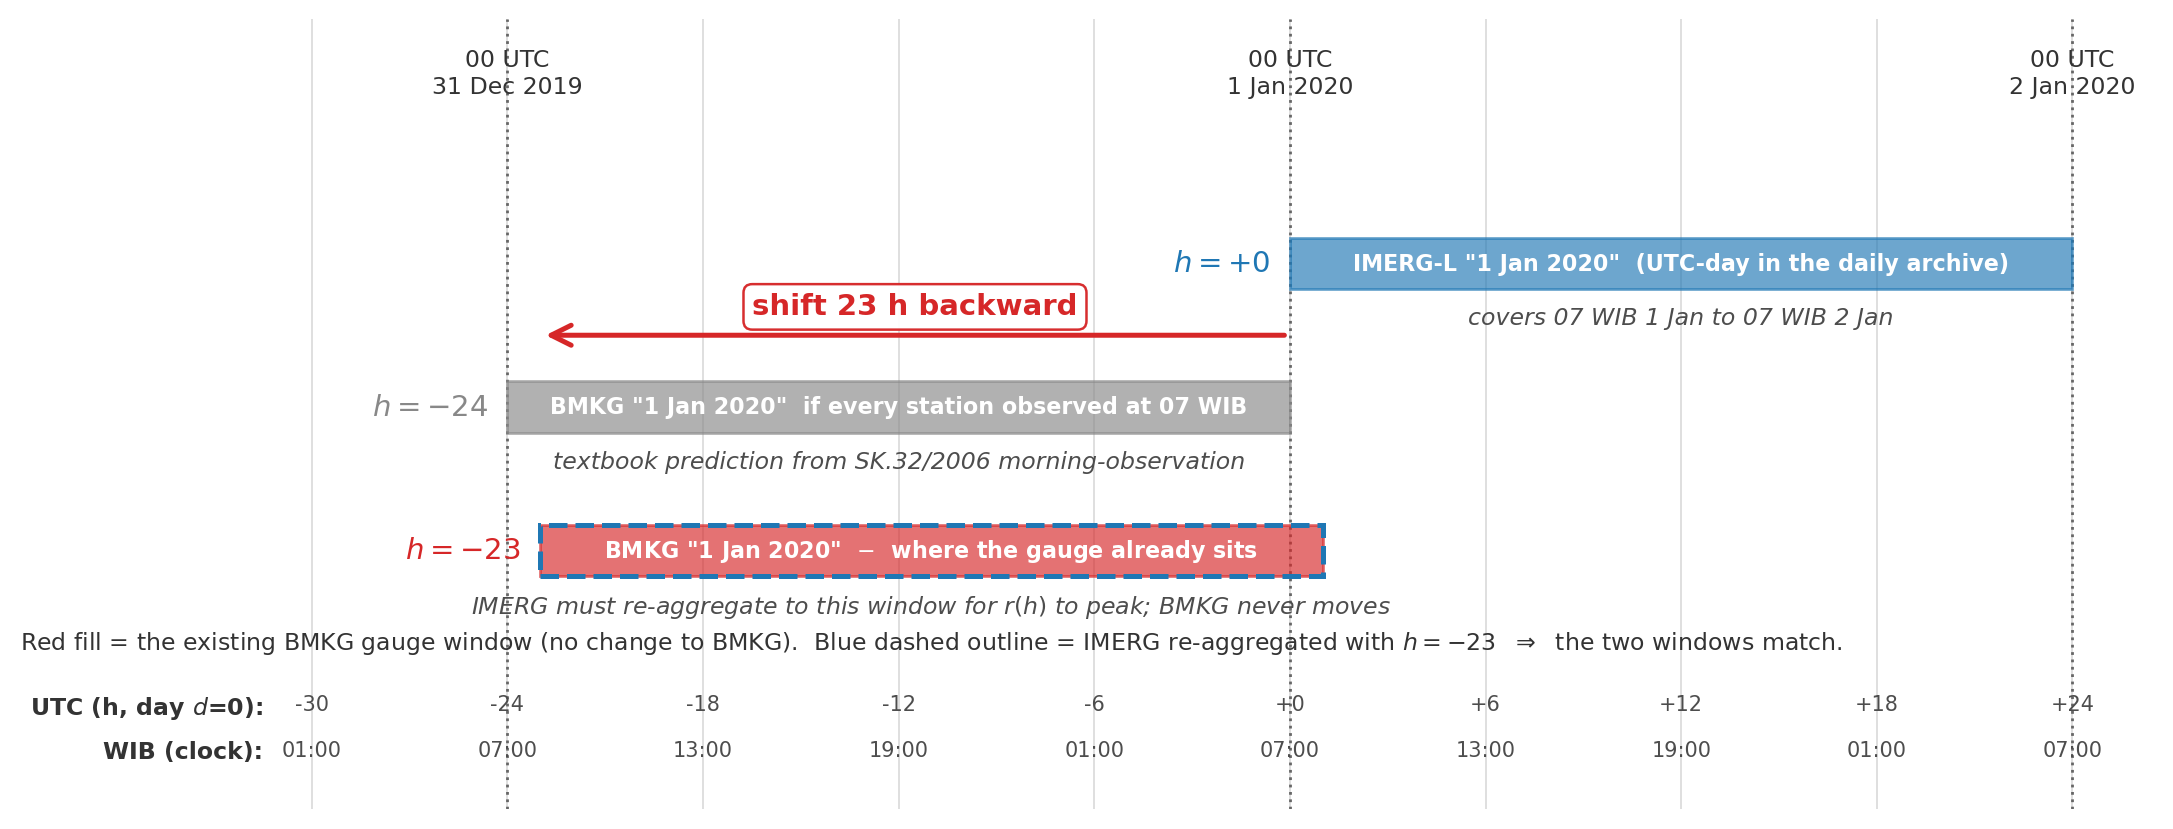
\includegraphics[width=\figThreeWindowWidth\textwidth]{fig_thesis_03_window_schematic.png}
\caption[Why a $-23$ h window aligns the satellite with the BMKG gauge day]{Why a $-23$~h window aligns the satellite with the BMKG gauge day.\label{fig:window-schematic}}
\end{figure}

Because marginal correction preserves the rank order of the daily
series, the correlation is essentially invariant to the LSEQM+DL
stages (Section~\ref{sec:discussion-bound}). The diagnostic is
therefore computed on the raw half-hourly retrieval rather than on
the corrected product, which isolates the window contribution
without re-running the pipeline at each of the $97$ offsets. The
correlation is pooled through additive sufficient statistics, so
that any aggregation, by pooled station-day pairs, by timezone
band, by calendar month, or by three-month running season, follows
without recomputation. Two poolings are reported: the full BMKG
record ($2001$ to $2021$, the span of the half-hourly archive
processed for the window diagnostic), which resolves the
dependence of the recovery on the satellite era, and the GPM era ($2015$ to $2021$),
which gives the seasonal and per-station climatology over the
years in which IMERG resolves the diurnal cycle. Timezone bands
use the operational WIB, WITA, and WIT assignment ($\text{UTC}+7$,
$+8$, $+9$) recorded for each station.

A monthly re-validation aggregates the daily totals at the
UTC-day and the matched windows into monthly sums and compares
them against the BMKG monthly totals. A station-month is retained
only when no more than five daily values are missing, so that each
monthly total rests on near-complete coverage. This tests whether
the window dependence of the daily correlation survives temporal
aggregation.


% ------------------------------------------------------------
\section{Reproducible Implementation Design}\label{sec:methods-reproducibility}
% ------------------------------------------------------------

The first three sections describe the pipeline as an algorithm.
This section describes it as a software artefact. Reproducibility
is treated here as a parallel methodological contribution of the
thesis: every result reported in Chapter~\ref{chap:results} maps
to a specific function in the source codebase, a specific cell
in a numbered notebook, and a specific configuration value in
\texttt{config.yml}. The empirical demonstration of end-to-end
re-runnability is given in
Section~\ref{sec:results-reproducibility}; this section
describes the design that supports it.

\subsection{Module Architecture}

The Python implementation is partitioned into ten modules under
\texttt{src/}, each with a single responsibility:
\texttt{config} (path and parameter resolution),
\texttt{io} (NetCDF and CSV input and output),
\texttt{utility} (land-mask, lat-flip, sentinel handling),
\texttt{bias\_correction} (LS and EQM stages),
\texttt{distribution\_fitting} (Gamma and GPD parameter
estimation via maximum likelihood, with the subsample-averaging
aggregator for small exceedance samples),
\texttt{deep\_learning} (CNN architecture, training loop, and
inference),
\texttt{station\_density} (confidence-mask construction),
\texttt{metrics} (the 31-metric verification catalogue),
\texttt{qa\_framework} (Composite Quality Index assembly), and
\texttt{station\_validation} (per-station extraction and
pairing). Each module is importable and exposes a small number
of named entry points; no inline function definitions appear in
the notebooks.

\subsection{Configuration-Driven Design}

All paths and parameters are declared in a single YAML file at
the project root, \texttt{config.yml}. A loader,
\texttt{initialize\_config()}, resolves placeholders such as
\texttt{\{main\_dir\}}, \texttt{\{input\_dir\}}, and
\texttt{\{output\_dir\}} to absolute paths at run time. The
sensitivity parameters acknowledged earlier in this chapter
($\alpha = 0.70$, the 80th-percentile GPD threshold, and
$c_{\text{sat}} = 2$) are exposed as named entries in
\texttt{config.yml}, so a sensitivity sweep is a configuration
edit followed by a re-run, with no code changes. The same
configuration file controls the dataset paths, the output
directory layout, the metric pillars, the CNN architecture
hyperparameters, and the per-method output filenames.

\subsection{Notebook Workflow}

The pipeline is exposed through six numbered Jupyter notebooks
under \texttt{notebooks/}: 01 (data acquisition), 02 (LSEQM+DL
bias correction), 03 (performance measurement), 04 (QA
framework), 05 (QA visualisation), and 06 (station validation).
Each notebook follows a
consistent style: short Markdown section headers, small code
cells with a single concern per cell, and calls into the
\texttt{src/} modules rather than inline implementations. The
batch-execution cells at the end of each notebook loop over the
36 dekadal windows with \texttt{try-except} guards so that a
failure in one window does not interrupt the others. The same
notebook can be opened in a local Jupyter installation or in
Google Colab; the behaviour is the same because the configuration
file is identical across environments.

\subsection{Documentation Site}

The \texttt{docs/} directory is a Quarto project that serves as
the documentation site for the framework. The site is structured
into sections that mirror this chapter: \textit{get-started},
\textit{methodology}, \textit{implementation}, \textit{technical},
\textit{example (Bali)}, and \textit{FAQ}. Each documentation page
is cross-linked to the specific notebook cell and source-code
function it describes, so a reader following the documentation can
move directly to the runnable artefact and back. The source code,
notebooks, and documentation are released openly on GitHub under
the Mozilla Public License 2.0, and the full Indonesia input and
output data are deposited on Zenodo with a citable DOI
(Appendix~\ref{app:code}); the documentation site is the
recommended entry point for any reader who wants to run or extend
the pipeline.

\subsection{Environment Specification}

The Python environment is declared in \texttt{environment.yml}
with pinned versions for the core scientific packages
(\texttt{numpy}, \texttt{xarray}, \texttt{scipy},
\texttt{scikit-learn}, \texttt{tensorflow}, \texttt{keras},
\texttt{lmoments3}). The environment was tested on a Windows
local installation with a Conda environment named
\texttt{climate}. Hardware-dependent paths in the CNN training
step are auto-detected at runtime.

Together, these five elements (module architecture, configuration
file, numbered notebooks, documentation site, and
pinned environment) form the reproducibility design of the
framework. Section~\ref{sec:results-reproducibility} demonstrates
that an end-to-end re-run from the published source reproduces
the headline numbers in Chapter~\ref{chap:results} to within the
floating-point tolerance of the underlying libraries.


% ------------------------------------------------------------
\section*{Chapter summary}
% ------------------------------------------------------------

This chapter described the LSEQM+DL pipeline in algorithmic
form and as a software artefact. The four-stage pipeline matches
one correction stage to each of the three marginal-distribution
bias dimensions (LS for the mean, EQM with Gamma for the bulk,
GPD for the tail) and adds a spatial-refinement stage (CNN) for
the extreme pixels. A station-density-aware blending step
modulates the CNN contribution by local gauge density, so the
pipeline degrades gracefully to LSEQM in regions where the
reference is weak. The implementation is partitioned into
single-responsibility modules, driven by a single configuration
file, exposed through six numbered notebooks, and documented
through a Quarto site. Validation against 172 out-of-sample BMKG stations
pools across 36 dekadal windows and 25 years to give the sample
size needed for stable distribution fits and small noise floors
on the headline metrics. The 31-metric verification catalogue is
grouped into four pillars and a separately-reported temporal-skill
diagnostic; the four pillars are the metrics the pipeline is
designed to move, and the temporal-skill diagnostic is the metric
the pipeline is not designed to move. The Chapter~\ref{chap:results}
results are organised around this division.

% ============================================================
% chapter_04_results.tex - Chapter 4, Results
%
% Purpose: reports the empirical performance of the LSEQM+DL framework
%          against 172 independent BMKG stations across the four
%          verification pillars + temporal-skill diagnostics.
% Sections: 4.1 Agreement Among the Three Datasets,
%           4.2 Stage-wise Headline Skill, 4.3 Stage-wise Attribution,
%           4.4 Threshold-Dependent Detection,
%           4.5 Pearson Correlation Across Stages,
%           4.6 Spatial Skill Distribution, 4.7 Per-Station Taylor Diagram
%           Analysis, 4.8 Temporal Stability Across Dekads,
%           4.9 Sensitivity Analyses, 4.10 Reproducibility Evaluation,
%           4.11 Chapter summary.
% Included by main_thesis.tex.
% License: CC BY 4.0 (see ../LICENSE).
% ============================================================

\chapter{RESULTS}\label{chap:results}

This chapter reports the empirical performance of the LSEQM+DL
framework (Linear Scaling, Empirical Quantile Mapping, Generalized
Pareto Distribution, and a Convolutional Neural Network refinement)
against 172 independent BMKG stations, pooled across
the 36 dekadal windows of 2001 to 2021. The results are organised
around the four-pillar verification framework introduced in
Section~\ref{sec:methods-metrics}, with the temporal-skill
diagnostic of Pearson correlation reported separately because of
the structural distinction that
Chapter~\ref{chap:discussion} develops.

Section~\ref{sec:results-intercomparison} first compares the three
datasets with each other, before any correction, and separates
their genuine disagreement from the calendar label each archive
assigns.
Section~\ref{sec:results-headline} presents the headline
stage-wise skill across the four pillars.
Section~\ref{sec:results-stages} attributes each metric movement
to the pipeline stage that produced it.
Section~\ref{sec:results-threshold} reports the
threshold-dependent detection results that the aggregate
event-detection numbers in
Section~\ref{sec:results-headline} mask.

Section~\ref{sec:results-correlation} reports the Pearson
correlation across stages and the paradox at the centre of the
discussion.
Section~\ref{sec:results-window} returns to the calendar theme of
Section~\ref{sec:results-intercomparison} at half-hourly
resolution, locating the optimal aggregation window; the two are
independent measurements of the same effect and agree. The
remaining sections cover the spatial skill
distribution (Section~\ref{sec:results-cqi}), per-station Taylor
analysis (Section~\ref{sec:results-taylor}), temporal stability
across dekads (Section~\ref{sec:results-temporal}), sensitivity
analyses on the framework parameters
(Section~\ref{sec:results-sensitivity}), and the reproducibility
evaluation that demonstrates end-to-end re-runnability
(Section~\ref{sec:results-reproducibility}).


% ============================================================
\section{Agreement Among the Three Datasets}\label{sec:results-intercomparison}
% ============================================================

The correction pairs a satellite product with a gridded gauge
reference and is judged against an independent station network, so
the three datasets are compared with each other before the
correction results are presented. Two questions are settled here:
how closely the three agree at the daily scale, and how much of any
disagreement belongs to the data rather than to the calendar label
each archive assigns. The corrected stages are then put through the
same comparison, which separates the two effects.

Every satellite-versus-BMKG correlation in this section is
constructed the same way, and differently from the rest of the
chapter. It uses daily paired values, taken as a single pooled
correlation over all station-days rather than sliced into
dekad-of-year windows, over the continuous GPM-era record from 2015
to 2021, against the $177$ BMKG stations that carry at least $100$
valid paired days in that window. The grid-to-grid
pairs reported below, IMERG-L against CPC-UNI and the corrected
fields against IMERG-F, are necessarily constructed differently
and are qualified where they are quoted. That count sits
between the $172$ stations used for the dekadal correction metrics
(Section~\ref{sec:results-headline}) and the $178$ used for the
half-hourly window diagnostic (Section~\ref{sec:results-window});
the three differ only in the coverage each analysis requires.
Full-record values are reported alongside throughout, because the
two eras differ substantially.

Because these values are constructed differently from the
correlations reported elsewhere in the thesis, they do not match
them, and the differences are systematic rather than
contradictory. Three constructions recur. The in-sample figure of
$0.348$ quoted in Section~\ref{sec:results-correlation} is measured
per pixel against the CPC-UNI calibration target, not against the
stations. Against the BMKG stations over the full record the same
corrected product gives $0.280$; slicing that record into the $36$
dekad-of-year windows used for the correction metrics removes the
seasonal cycle and lowers it to $0.235$; restricting instead to the
GPM era lowers it to $0.174$. Each step changes the construction
in more than one respect, stratification and pooling together, so
the values are not directly comparable; the reference, the record,
the stratification, the pooling, and the window label must all be
carried with any correlation quoted from this work.

\subsection{Agreement Under the Archived Date Labels}

Under the date label each archive carries, the three daily
correlations split sharply. The two UTC-dated products, IMERG-L and
CPC-UNI, agree with each other at $r = 0.57$, measured between the
two gridded archives at the $178$ station locations rather than
against the station records themselves. Each agrees with the
independent BMKG network far less: $0.195$ for IMERG-L and $0.154$
for CPC-UNI. That a gauge analysis assembled from station reports
should agree with an independent station network no better than a
raw satellite retrieval does is not a credible statement about data
quality; it points instead at the date label, which the two gridded
archives share and the BMKG network, reporting on the local
morning-observation day, does not.

\subsection{Agreement After Harmonising the Date Label}

Shifting each gridded series by whole days against the BMKG date
resolves the discrepancy. Every product peaks at a shift of
$-1$~day, the offset implied by the morning-observation convention:
the BMKG total dated~$d$ accumulates over the 24~hours ending at
the morning observation on~$d$ and therefore covers mostly rain
that fell on the previous calendar day. At that shift the
correlation rises to $0.751$ for CPC-UNI, a factor of $4.9$, and to
$0.568$ for IMERG-L, a factor of $2.9$, for a change that alters no
precipitation value.

The recovery is specific to the GPM era, and the reason is
instructive. Splitting the record at the arrival of the full GPM
constellation, the pre-GPM years of 2001 to 2013 give $0.358$ for
IMERG-L at the archived label against $0.320$ at the $-1$~day
label, a difference of little consequence, whereas the GPM years
give $0.195$ against $0.568$. The earlier product does not resolve
the diurnal cycle, so its daily total is temporally smeared and
correlates moderately whichever 24-hour window is used; the later
product resolves timing sharply and therefore correlates strongly
at the matched window and poorly at the mismatched one. Improved
retrieval timing makes a product more sensitive to a calendar
error, not less. The consequence for reporting is that the full
record sits between the two eras at both labels, so a correlation
against BMKG quoted without its era is ambiguous by roughly
$0.10$. This day-resolution result reproduces the flat pre-GPM
behaviour that the half-hourly diagnostic of
Section~\ref{sec:results-window} finds independently.

This day-label scan and the half-hourly window diagnostic of
Section~\ref{sec:results-window} are independent measurements and
they agree closely. The daily IMERG-L archive at zero shift gives
$0.1951$, against the $0.1949$ obtained by re-accumulating the
half-hourly source at $h = 0$; at the matched label the two give
$0.568$ and $0.571$. The small residual is expected, since the day
scan resolves no finer than $-24$~h while the half-hourly scan
places the optimum at $-23$~h, and the two pool marginally different
station sets. CPC-UNI evaluated on its native $0.5^{\circ}$ grid and
on the regridded $0.1^{\circ}$ grid agree to within $0.003$
($0.751$ and $0.749$ at the $-1$~day label), so the regridding step
carried out inside the pipeline does not affect this comparison.

The third pair completes the matrix from the other direction.
Table~\ref{tab:pairwise-daylabel} scans the two satellite-versus-gauge
pairs across date labels. The IMERG-L against CPC-UNI pair is scanned
instead across accumulation windows, because both archives are gridded
and neither carries a station reporting convention to shift; that scan
is reported in Chapter~\ref{chap:discussion}
(Table~\ref{tab:convention}), and it completes the diagonal: each
reference peaks at its own window and falls away at the other.

\subsection{What the Harmonised Values Do and Do Not Show}

At the $-1$~day label CPC-UNI reaches $0.751$ against BMKG while
IMERG-L reaches $0.568$. This gap is not a skill comparison.
CPC-UNI is a gauge analysis assembled from station reports
distributed over the Global Telecommunication System, and, as
Section~\ref{sec:methods-reference-quality} sets out, the
Indonesian contributions to that stream originate from BMKG. At the matched label the
reference is therefore partly reproducing the observations against
which it is being scored, and the per-station median at that label,
$0.865$, sits above the pooled value in a way that is consistent
with that shared origin.

Two conclusions follow. First, the low correlation between CPC-UNI
and BMKG under the archived labels is a calendar artefact rather
than a defect in the reference: harmonise the label and the two
gauge datasets agree closely. Second, and for the same reason,
CPC-UNI cannot serve as an independent check on a product
calibrated against it. The out-of-sample validation against BMKG
reported through the rest of this chapter is a requirement of the
design, not a supplementary test.

\subsection{The Same Comparison After Correction}

Repeating the scan on the three corrected stages separates the
calendar effect from the correction. Under the same construction
the correlation against BMKG moves from $0.195$ for the raw archive
to $0.198$, $0.173$, and $0.174$ for LS, LSEQM, and LSEQM+DL under
the archived label, and from $0.568$ to $0.569$, $0.552$, and
$0.555$ at the $-1$~day label (Table~\ref{tab:pairwise-daylabel}).
Two points follow.

No stage materially improves day-to-day timing at either label. LS
sits $0.003$ above the raw archive at the archived label and $0.001$
above it at the $-1$~day label, differences that are at the edge of
the sampling uncertainty for this sample size, and the two later
stages fall slightly below the raw archive at both. This closes an
objection that the archived-label numbers alone cannot answer: that
the flat correlation reported against the independent stations
might be an artefact of misaligned dates concealing a real gain. It
is not. With the dates aligned the corrected product still does not
separate from the raw archive. The corresponding in-sample result
against CPC-UNI is reported separately in
Section~\ref{sec:results-correlation} and
Table~\ref{tab:headline-cpc}, where the correction is likewise flat
but the values sit near $0.348$, being measured per pixel against the
calibration target rather than pooled over station-days at the gauges.

The calendar effect is independent of the correction. Every stage
retains the lift at $-1$~day, so the relabelling can be applied
before or after the pipeline for the same benefit. A separate
comparison supports the same reading: measured per pixel and
averaged over the $36$ dekadal windows of the full record, the
corrected fields correlate with the raw IMERG-F Final run at
$0.955$, $0.935$, and $0.936$ for the three stages, so the
correction rescales the field without restructuring its day-to-day
pattern.

\begin{table}[H]
\centering
\caption[Daily correlation against BMKG under two date labels]{Daily
Pearson $r$ against the $177$ BMKG stations, as a single pooled
correlation over the continuous record, under the archived date
label and after a $-1$~day shift; $n$ is $2.9\times10^{5}$ paired
station-days in the GPM era and $8.7\times10^{5}$ over the full
record.\label{tab:pairwise-daylabel}}
\begingroup\small
\begin{tabular*}{\textwidth}{@{\extracolsep{\fill}}lcccc@{}}
\toprule
& \multicolumn{2}{c}{GPM era, 2015 to 2021}
& \multicolumn{2}{c}{Full record, 2001 to 2021} \\
\cmidrule(lr){2-3}\cmidrule(lr){4-5}
Product & Archived & $-1$~day & Archived & $-1$~day \\
\midrule
IMERG-L (raw)   & 0.195 & 0.568 & 0.295 & 0.405 \\
LS              & 0.198 & 0.569 & 0.299 & 0.415 \\
LSEQM           & 0.173 & 0.552 & 0.276 & 0.403 \\
LSEQM+DL        & 0.174 & 0.555 & 0.279 & 0.406 \\
\addlinespace
CPC-UNI         & 0.154 & 0.751 & 0.332 & 0.532 \\
\bottomrule
\end{tabular*}
\endgroup
\end{table}


% ============================================================
\section{Stage-wise Headline Skill}\label{sec:results-headline}
% ============================================================

Each correction stage was designed to address a distinct bias
dimension, and the verification organises around the same
taxonomy. Ten metrics in Table~\ref{tab:headline} group into the
four pillars introduced in Section~\ref{sec:methods-metrics}:
\textit{value adjustment} (relative bias (RB), standard deviation
ratio (SDR)), \textit{distribution alignment} (Kolmogorov-Smirnov (KS) $p$-value, wet-day
frequency, wet-day intensity), \textit{extreme preservation}
($Q_{95}$ and $Q_{99}$ ratios), and \textit{event detection}
(Probability of Detection (POD), Critical Success Index (CSI), False Alarm Ratio (FAR)). Reading down a column gives the per-stage
performance; reading across pillars gives the design coverage of
the framework.

The table is reported stage-by-stage rather than
only as raw-versus-corrected so that each column can be audited
against the bias dimension its stage was designed to address. If
LS over-corrects the mean, the LS column will reveal it; if EQM
under-aligns the bulk distribution, the LSEQM column will too;
and if the CNN distorts a metric outside its operating range,
the LSEQM+DL column will show that as well. All numbers are
pooled across the 36 dekadal windows of 2001 to 2021 at the 172
BMKG stations not used in any correction step, so the comparison
tests whether the corrections generalise beyond the Climate
Prediction Center (CPC) Unified Gauge-Based Analysis of Global
Daily Precipitation (CPC-UNI) training reference.

\begin{table}[H]
\centering
\caption[Stage-wise skill against 172 independent BMKG stations]{Stage-wise skill against 172 independent BMKG stations,
pooled across all 36 dekads (2001 to 2021)\label{tab:headline}}
\begingroup\small
\begin{tabular}{@{}llcccc@{}}
\toprule
Pillar & Metric & LS & LSEQM & LSEQM+DL & Target \\
\midrule
Value Adjustment
  & Relative Bias        & $-$0.114 & 0.009 & \textbf{$-$0.006} & 0 \\
  & SDR                  & 0.71 & 1.03 & \textbf{1.00} & 1.0 \\
Distribution Alignment
  & KS $p$-value (\%)    & 0.01 & \textbf{19.07} & \textbf{19.07} & 100 \\
  & Wet-Day Freq.\ Ratio & 1.21 & \textbf{0.96} & 0.95 & 1.0 \\
  & Wet-Day Int.\ Ratio  & 0.71 & 1.06 & \textbf{1.05} & 1.0 \\
Extreme Preservation
  & $Q_{95}$ Ratio       & 0.74 & 1.07 & \textbf{1.05} & 1.0 \\
  & $Q_{99}$ Ratio       & 0.71 & 1.05 & \textbf{1.01} & 1.0 \\
Event Detection
  & POD                  & \textbf{0.78} & 0.65 & 0.65 & 1.0 \\
  & CSI                  & \textbf{0.53} & 0.49 & 0.49 & 1.0 \\
  & FAR                  & 0.36 & \textbf{0.32} & \textbf{0.32} & 0 \\
\bottomrule
\end{tabular}
\endgroup
\end{table}

Table~\ref{tab:headline} reports the out-of-sample skill against
the 172 BMKG validation stations, which is the strongest claim
the framework supports because the BMKG network is independent
of the correction reference. Bold values mark the best
performance per row, and the target column gives the value for
perfect agreement with observations. The parallel paper
\citep{ref:istanto2026mdpi}\MDPIstatus reports a companion table
of in-sample skill against the CPC-UNI calibration target;
Table~\ref{tab:headline-cpc} reproduces those values here so the
two-tier validation framework of
Section~\ref{sec:methods-validation} can be read in full. In its
temporal-skill rows, RMSE is the root mean square error and NSE
is the Nash-Sutcliffe efficiency.

\begin{table}[H]
\centering
\caption[In-sample skill against the CPC-UNI calibration target]{In-sample skill against the CPC-UNI calibration target,
pooled across all 36 dekads (2001 to 2025)\label{tab:headline-cpc}}
\begingroup\small
\begin{tabular}{@{}llcccc@{}}
\toprule
Pillar & Metric & LS & LSEQM & LSEQM+DL & Target \\
\midrule
Value Adjustment
  & Relative Bias        & \textbf{0.000} & 0.070 & 0.065 & 0 \\
  & SDR                  & \textbf{0.971} & 1.159 & 1.148 & 1.0 \\
Distribution Alignment
  & KS $p$-value (\%)    & \textbf{6.56} & 0.00 & 0.00 & 100 \\
  & Wet-Day Freq.\ Ratio & \textbf{1.040} & 0.947 & 0.946 & 1.0 \\
  & Wet-Day Int.\ Ratio  & \textbf{0.961} & 1.157 & 1.152 & 1.0 \\
Extreme Preservation
  & $Q_{95}$ Ratio       & \textbf{0.946} & 1.171 & 1.163 & 1.0 \\
  & $Q_{99}$ Ratio       & \textbf{0.967} & 1.212 & 1.196 & 1.0 \\
Event Detection
  & POD                  & \textbf{0.767} & 0.707 & 0.707 & 1.0 \\
  & CSI                  & \textbf{0.589} & 0.572 & 0.572 & 1.0 \\
  & FAR                  & 0.271 & 0.248 & \textbf{0.248} & 0 \\
\midrule
Temporal Skill
  & Pearson $r$          & 0.343 & 0.345 & \textbf{0.348} & 1.0 \\
  & RMSE (mm/day)        & \textbf{13.10} & 14.18 & 14.07 & 0 \\
  & NSE                  & \textbf{$-$0.273} & $-$0.548 & $-$0.524 & 1.0 \\
\bottomrule
\end{tabular}
\endgroup
\end{table}

The two tables tell a complementary story. Against CPC-UNI
(Table~\ref{tab:headline-cpc}), LS has zero relative bias by
construction and the LSEQM/LSEQM+DL stages overshoot the
reference distribution slightly at the upper percentiles. Against
BMKG (Table~\ref{tab:headline}), LS retains a residual bias of
$-11.4\%$, dominated by the limit of a single multiplicative
correction that does not adjust distribution shape, with a smaller
contribution from the gauge-to-gauge offset between CPC-UNI and
BMKG; the stage-wise attribution below confirms the correction-side
contribution dominates. The LSEQM/LSEQM+DL stages move the corrected
product close to unity at every pillar. The apparent overshoot
of LSEQM+DL Q$_{99}$ ratio against CPC-UNI ($1.20$) becomes a
near-perfect match against BMKG ($1.01$): the framework was
calibrated to CPC-UNI but reproduces BMKG more accurately because
CPC-UNI itself under-catches heavy rain. The Temporal Skill
section of Table~\ref{tab:headline-cpc} is the basis for the
Pearson correlation analysis in
Section~\ref{sec:results-correlation}.

Reading across the four pillars against the independent BMKG
stations (Table~\ref{tab:headline}), the framework moves three
pillars cleanly toward the gauge target and produces a designed
trade-off in the fourth. Every skill value quoted in the four
paragraphs that follow is measured against BMKG. The value-adjustment pillar shows
LSEQM and LSEQM+DL essentially eliminating the LS residual:
relative bias moves from $-11.4\%$ under LS to $+0.9\%$ under
LSEQM and $-0.6\%$ under LSEQM+DL, leaving the corrected product
within one percentage point of the gauge target. The standard
deviation ratio (SDR) tracks the same path, from $0.71$ (a $29\%$
spread compression under LS) through $1.03$ (slight over-spread
under LSEQM) to exactly $1.00$ under LSEQM+DL, where the CNN
refinement pulls the EQM overshoot back to the gauge target.

The distribution-alignment pillar shifts from rejection at the
$99.99\%$ level under LS ($p = 0.01\%$) to acceptance at
conventional confidence levels under LSEQM and LSEQM+DL ($p =
19.1\%$), meaning the corrected daily distributions are no
longer statistically distinguishable from the gauge reference.
The wet-day frequency ratio echoes the move, from $1.21$ (a
$21\%$ over-count of rainy days under LS, consistent with the
Integrated Multi-satellitE Retrievals for Global Precipitation Measurement (IMERG) tendency to over-detect drizzle and light rain) to $0.96$
and $0.95$ under LSEQM and LSEQM+DL respectively, indicating
that the dry-day-matching mechanism has done its work without
introducing a counter-bias. The wet-day intensity ratio moves
in parallel from $0.71$ under LS to $1.06$ under LSEQM and
$1.05$ under LSEQM+DL, confirming that the mean rainfall on wet
days now matches the gauge magnitude after the bulk-distribution
correction.

The extreme-preservation pillar recovers the upper tail that LS
truncates by construction. $Q_{99}$ moves from $0.71$ (a $29\%$
under-prediction of heavy-rain magnitude) through $1.05$ under
LSEQM (a slight overshoot from the EQM tail extrapolation) to
$1.01$ after CNN refinement, and $Q_{95}$ follows the same arc
($0.74 \rightarrow 1.07 \rightarrow 1.05$). The CNN stage acts
as a tail trim, pulling the EQM overshoot back toward unity
rather than amplifying it. This refinement is confined to a small
extreme-tail footprint, modifying under a fifth of land pixel-days
and predominantly downward, quantified in
Figure~\ref{fig:cnn-footprint} below.

The event-detection pillar reveals the expected trade-off.
Matching the dry-day frequency suppresses spurious light-rain
events, which lowers aggregate POD from $0.78$ to $0.65$ and
CSI from $0.53$ to $0.49$ but also reduces FAR from $0.36$ to
$0.32$. The aggregate numbers in
Table~\ref{tab:headline} mask a threshold-dependent reversal
that Section~\ref{sec:results-threshold} details: skill loss
is concentrated at light-rain thresholds where false alarms
drive the count, while skill at heavy-rain thresholds improves
substantially. Figure~\ref{fig:headline-bars} presents one
representative metric per pillar in bar form, with LS, LSEQM,
and LSEQM+DL side-by-side and the perfect-agreement target
marked.

\begin{figure}[H]
\centering
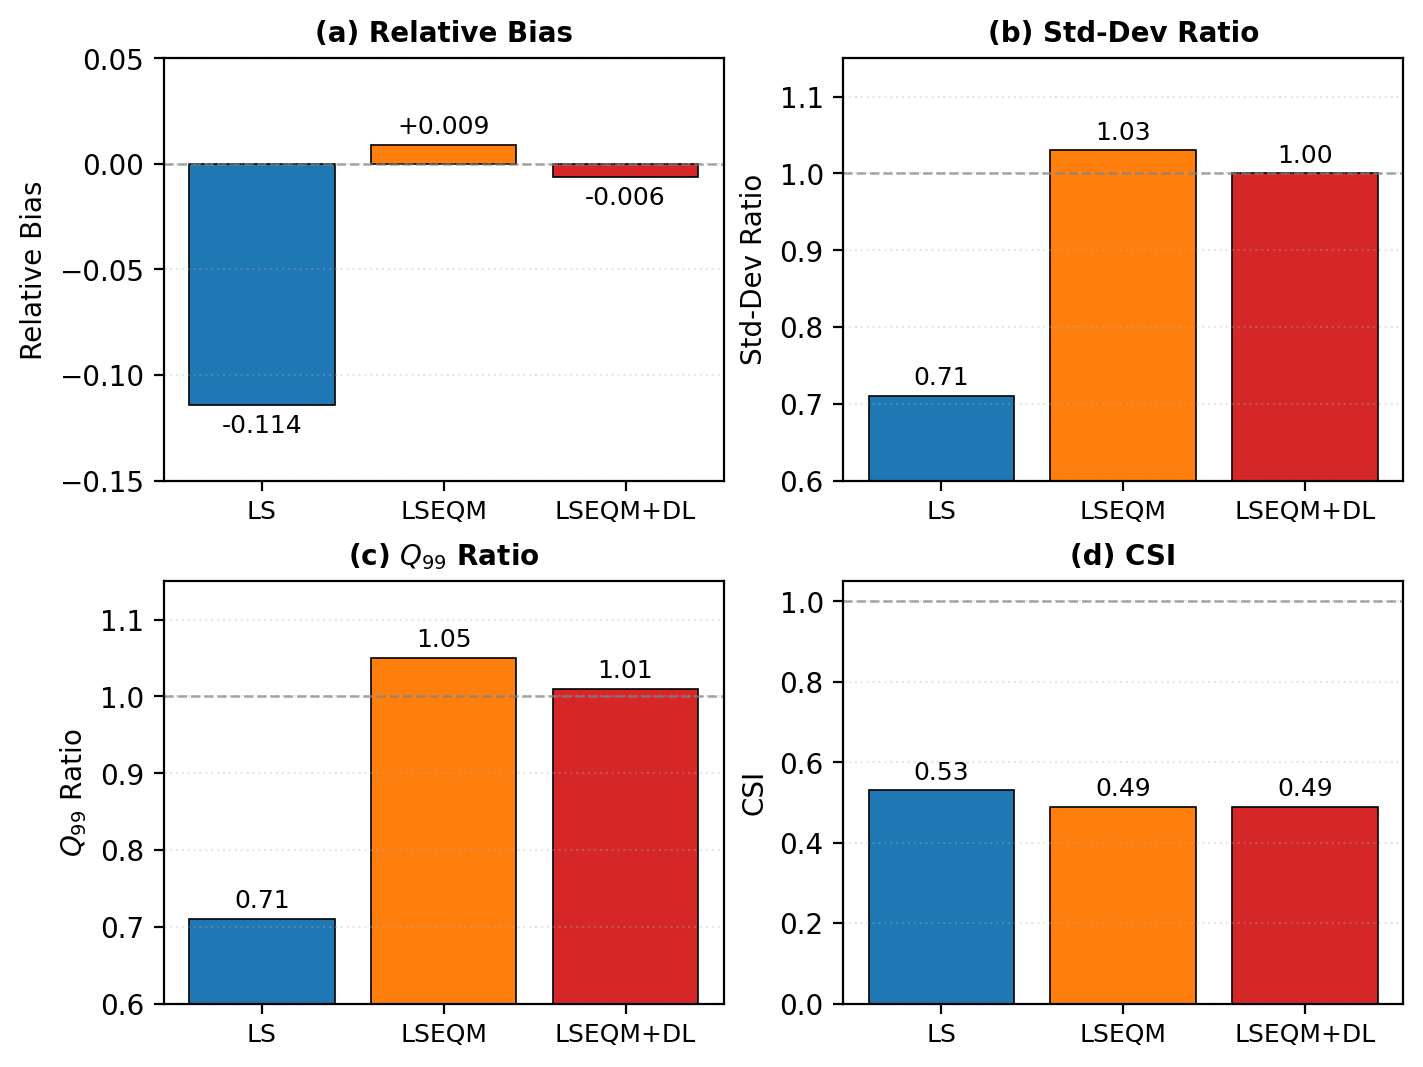
\includegraphics[width=\figFourOneWidth\textwidth]{fig_thesis_04_headline_bars.png}
\caption[Stage-wise skill at 172 BMKG stations for four representative metrics]{Stage-wise skill at 172 independent BMKG stations for
four representative metrics drawn from
Table~\ref{tab:headline}\label{fig:headline-bars}}
\end{figure}

A single-day spatial example of all six products on $1$~January~$2025$,
including the raw IMERG-L, the three correction stages, the IMERG
Final Run (IMERG-F) independent benchmark, and the CPC-UNI gauge
reference, is in
Appendix~\ref{app:atlas}~Figure~\ref{fig:atlas-six}.


% ============================================================
\section{Stage-wise Attribution}\label{sec:results-stages}
% ============================================================

The three correction stages can be read as an additive sequence,
each addressing a residual that the previous stage cannot reach.
This section walks through the stages in order and reports, for
each, the evaluation metrics that shift and the magnitude of the
shift, before the threshold-stratified detection analysis in
Section~\ref{sec:results-threshold} unpacks the apparent
event-detection regression seen in the aggregate.

\subsection*{What Linear Scaling Achieves}

Linear Scaling is the simplest correction in the pipeline, and
its performance against BMKG reflects what a single
mean-rescaling step can and cannot do. The relative bias against
BMKG of the LS-corrected field is $-11.4\%$. LS was designed to
match the dekadal mean against CPC-UNI, not against BMKG, so its
BMKG-side residual reflects two contributions: the limited
correction (a single multiplicative factor that does not adjust
distribution shape) and the gauge-to-gauge offset between the
CPC-UNI gridded analysis and BMKG point measurements
\citep{ref:chen2008}. The decomposition between these two
contributions can be inferred from the next subsection: the
LSEQM stage uses the same CPC-UNI training and brings the BMKG
residual to $+0.9\%$, indicating that the correction-side
contribution dominates and that the residual is not a pure
reference offset.

The standard deviation ratio against BMKG sits at $0.71$,
indicating that the corrected satellite field still varies less
than the gauge observations. The distribution shape is
essentially unchanged: the Kolmogorov-Smirnov test against the
BMKG distribution returns $p = 0.01\%$, far below conventional
acceptance thresholds. The wet-day frequency ratio of $1.21$
confirms that LS retains the IMERG Late Run (IMERG-L) tendency to over-detect
light rain. LS also leaves the upper tail truncated: $Q_{99}$
stands at $0.71$, indicating that the satellite under-predicts
the heaviest events by a factor of about $0.71$. The qualitative
picture is consistent with what LS was designed for: it adjusts
the mean of the dekadal field but does not modify day-by-day
distributional structure. Stages 2 and 3 of the pipeline are
introduced precisely to address this gap.

\subsection*{What LSEQM Adds: the Largest Single Jump}

The LS-to-LSEQM transition produces the largest single
improvement in the framework across all three pillars except
event detection. The standard deviation ratio moves from $0.71$
to $1.03$, correcting a $29\%$ underestimation of observed
variability. The Kolmogorov-Smirnov $p$-value rises from
$0.01\%$ to $19.1\%$, so the corrected and BMKG distributions
can no longer be rejected as different populations at
conventional confidence levels \cite{ref:ebert2007, ref:wilks2020}. The wet-day frequency ratio drops from $1.21$ to
$0.96$, removing nearly all of the $21\%$ overestimation of
wet-day occurrence through the dry-day frequency matching
scheme. The $Q_{99}$ ratio improves from $0.71$ to $1.05$ and
the $Q_{95}$ ratio from $0.74$ to $1.07$, recovering the heavy
tail that LS truncates by construction. The relative bias
against BMKG flips sign and shrinks to $+0.9\%$, because gamma
EQM rescales the full distribution rather than only the mean.

Two costs accompany these gains. The probability of detection
(POD) drops from $0.78$ to $0.65$ and the critical success
index (CSI) from $0.53$ to $0.49$. Both follow from the dry-day
frequency matching design: when the corrected wet-day frequency
falls toward unity, a fraction of IMERG-L light-rain events
previously counted as hits are reclassified as dry. The
reclassification reduces over-detection and improves the false
alarm ratio (FAR) from $0.36$ to $0.32$, at the price of a
lower hit rate at low thresholds \citep{ref:maggioni2016}. The
trade-off is the intended outcome of the design choice;
Section~\ref{sec:results-threshold} shows where it is
favourable and where it is not.

A complementary reading of the same contingency table answers a
question operational users ask directly: on a day the gauge
records as dry, does the corrected product also report dry? Dry
days, those below the $1$~mm wet-day threshold, account for
$50\%$ of the validated station-days, so their treatment carries as
much weight as wet-day skill. Pooling the $1$~mm contingency table
over all station-dekads rather than averaging per-station rates,
the fraction of dry gauge days that the product
also reports dry rises from $56.2\%$ under Linear Scaling to
$69.3\%$ under LSEQM+DL, so the false-alarm rate on dry days
falls from $43.8\%$ to $30.7\%$. This is the dry-day counterpart
of the wet-day frequency ratio moving from $1.21$ to $0.95$: the
empirical quantile mapping reclassifies spurious light-rain pixels
to dry and removes the raw product's over-detection. The gain is
not free: it is the dry-day face of the same reclassification that
costs light-rain hits above.

\subsection*{What LSEQM+DL Adds: Tail Refinement}

The contribution of Stages~3 and 4 over the LSEQM baseline is
concentrated in the extreme tail. The $Q_{99}$ ratio sharpens
from $1.05$ to $1.01$, pulling the upper tail to within $1\%$
of the BMKG target; the $Q_{95}$ ratio tightens from $1.07$ to
$1.05$; and the SDR moves from $1.03$ to exactly $1.00$.
Distribution-alignment metrics (KS $p$-value, wet-day frequency
and intensity ratios) and event-detection metrics (POD, CSI,
FAR) are essentially unchanged because the CNN refinement
operates only above the $80$th-percentile threshold and does not
touch the bulk of the distribution.

The spatial footprint of the CNN confirms that it is a targeted
refinement rather than a whole-field rewrite.
Figure~\ref{fig:cnn-footprint} shows the share of land pixel-days
the CNN modifies in each year: on average $18.6\%$ over the
$2001$ to $2025$ record, confined to the pixels above the
$80$th-percentile tail. About two-thirds of the modified pixels
($67\%$) are adjusted downward, trimming the extreme overshoot the
Gamma and GPD extrapolation leaves behind, with a mean absolute
change of $0.36$~mm/day. These individually small, spatially
concentrated adjustments remove about four-fifths of the residual
$99$th-percentile overshoot while leaving the day-by-day pairing,
and hence Pearson~$r$, pinned close to its raw value
(Section~\ref{sec:discussion-bound}). The CNN thus acts only where
the statistical stages leave an incoherent residual in the
extremes, which is why it sits last in the pipeline.

\begin{figure}[H]
\centering
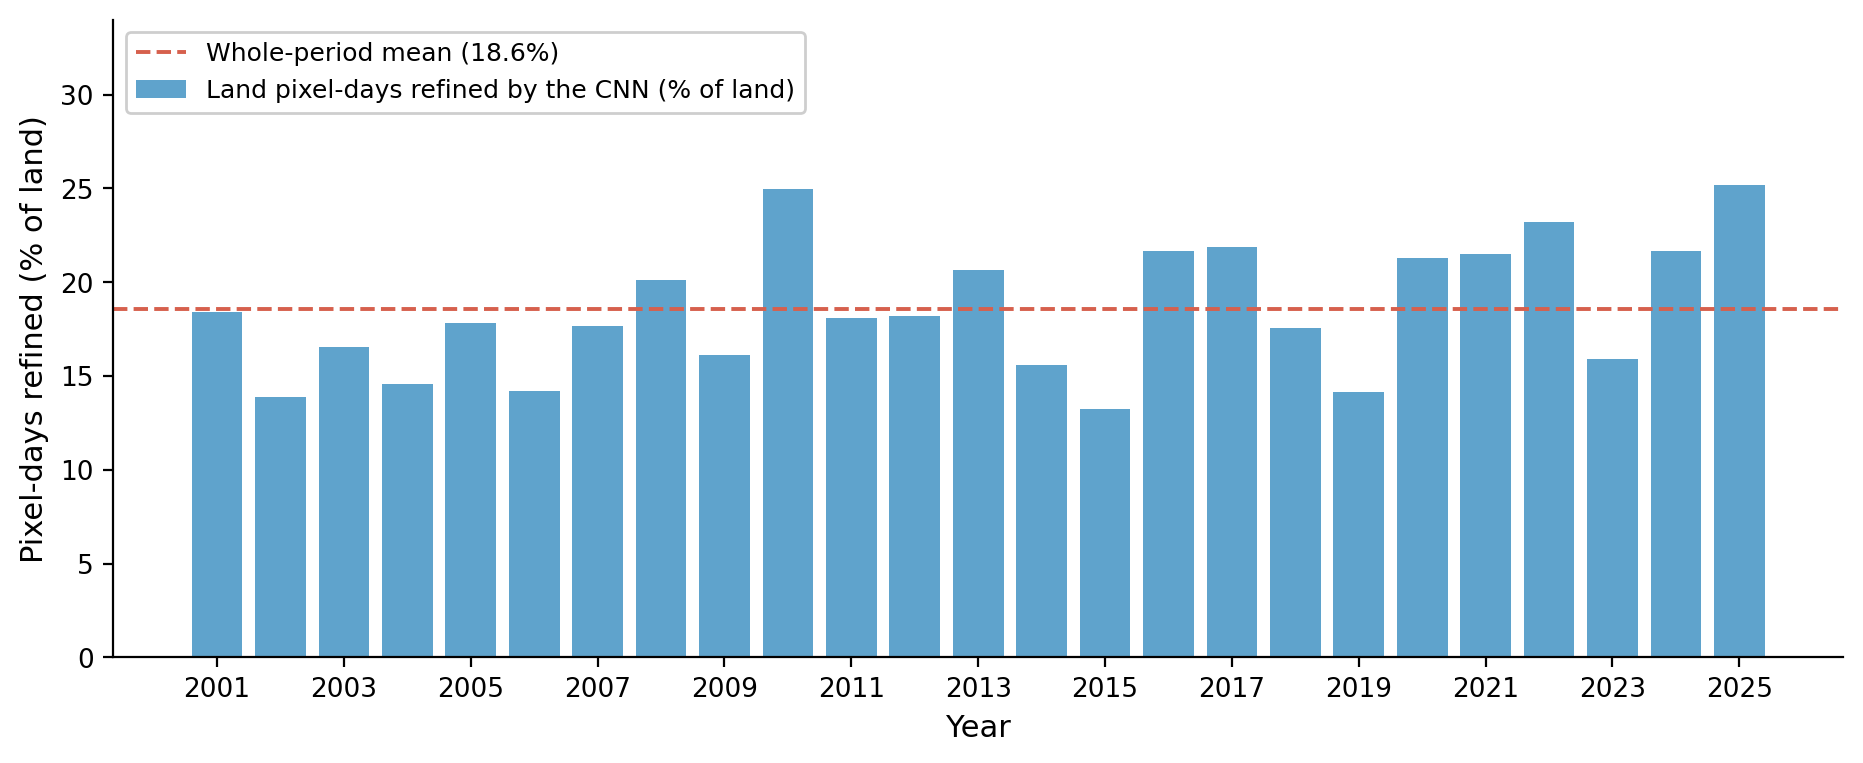
\includegraphics[width=\figFourCnnWidth\textwidth]{fig_thesis_I1_cnn_footprint.png}
\caption[CNN refinement footprint by year]{Share of land pixel-days the CNN modifies each year, with the whole-record mean; the CNN acts on a small extreme-tail footprint.\label{fig:cnn-footprint}}
\end{figure}

The stage-resolved attribution is therefore
complete: each stage moves the metrics matched to its design
dimension and leaves the others alone.
Appendix~\ref{app:atlas}~Figure~\ref{fig:atlas-diff} maps the
per-pixel residual on the same representative day, locating
where in the archipelago the correction is doing the most work.


% ============================================================
\section{Threshold-Dependent Detection}\label{sec:results-threshold}
% ============================================================

Daily precipitation over the region is strongly right-skewed, and
the correction has to act on that shape rather than on a
symmetric error. This section is reported against BMKG only: the
threshold-stratified contingency tables are accumulated at the
station points, and no gridded CPC-UNI equivalent exists.

Pooled over the daily BMKG station records at the satellite pixels
containing them, $2001$ to $2021$, wet-day
amounts have a skewness of $3.2$, the wettest $5\%$ of wet days
carry $26\%$ of the total and the wettest $1\%$ carry $8\%$, and
the $99$th wet-day percentile is $106$~mm/day against a
wet-day mean of $17$~mm/day. A heavy upper tail of this kind is
what the Generalized Pareto step of Stage~3 is included to
preserve; a Gamma fit alone underestimates the far tail of such a
distribution. The raw IMERG-L input departs from this reference
shape in two directions at once: it reports too many wet days (a
wet-day fraction of $0.61$ against $0.46$ for the gauges) while
truncating the heavy tail (a $99$th percentile of $73$~mm/day
against $106$). These are the two defects the threshold-stratified
verification exposes, and they move detection skill in opposite
directions as the threshold rises.

The aggregate event-detection metrics in
Table~\ref{tab:headline} mask a threshold-dependent reversal in
detection skill. Skill is broken out at a series of daily
thresholds in Figure~\ref{fig:threshold-skill}. Thresholds up to
$50$~mm/day follow the World Meteorological Organization (WMO)
multi-threshold verification practice \citep{ref:wmo1485,
ref:wmo1132}, while $100$ and $150$~mm/day are added as heavy and
extreme classes relevant to the Indonesian wet-season regime,
consistent with the WMO principle that extreme-precipitation
thresholds are set regionally \citep{ref:wmo1310}. The thresholds
are labelled here by their conventional daily-rainfall intensity
descriptors: $1$~mm (measurable), $5$~mm (light), $10$~mm
(moderate), $20$~mm (moderate-heavy), $50$~mm (heavy), and
$100$~mm (very heavy). The $150$~mm/day extreme class is omitted
because no station reaches the minimum of ten exceedances required
for stable categorical verification in any dekad of the record.

The two input defects account for the reversal. At the
$1$, $5$, and $10~\mathrm{mm/day}$ thresholds LS retains a higher
POD than LSEQM+DL. LS is a single multiplicative factor that leaves
the wet-day count untouched, so it keeps the raw over-detection of
light rain, and an over-detecting product scores more hits at a low
threshold. The distribution step of LSEQM+DL removes that
over-detection, reclassifying the spurious drizzle to dry, which
costs some of those low-threshold hits. The ordering changes only at
$20~\mathrm{mm/day}$, not at $5~\mathrm{mm/day}$.

Above the crossover the same two edits act the other way. LS
inherits the truncated tail, so it under-detects the heavy events
that sit above $20~\mathrm{mm/day}$. The empirical quantile
mapping and Generalized Pareto steps, by contrast, restore the upper tail from a
$99$th percentile of $73$ toward the gauge value of $106$~mm/day,
recovering heavy events the raw product places below the threshold.
The crossover between $10$ and $20~\mathrm{mm/day}$ is where the
loss of over-detected light rain and the recovery of the truncated
tail balance, and from $20~\mathrm{mm/day}$ upward LSEQM+DL
achieves the higher CSI at every resolved threshold.

At $50~\mathrm{mm/day}$ the median CSI is $0.091$ for LSEQM+DL
against $0.062$ for LS, a $45\%$ improvement, and the equitable
threat score (ETS), which removes the chance-hit contribution,
shows the same ordering. These two values are medians taken over
the $983$ station-dekad records that meet the ten-exceedance
minimum; Figure~\ref{fig:threshold-skill} instead averages the
per-dekad station medians, which raises the LSEQM+DL value to
$0.097$ and the improvement to $56\%$ without changing the
ordering. The $100~\mathrm{mm/day}$ class supports
no ordering: only $6$ of the $5{,}899$ station-dekad records reach
the ten-exceedance minimum, and the median CSI is zero for both
methods. The advantage is therefore established at $20$ and
$50~\mathrm{mm/day}$, where the record carries enough events.

The crossover threshold near $20~\mathrm{mm/day}$ is not an
arbitrary cut. It is the fixed threshold of R20mm, the
very-heavy-precipitation-day index of the World Meteorological
Organization Expert Team on Climate Change Detection and Indices,
defined as the annual count of days with precipitation at or above
$20~\mathrm{mm}$; the corresponding heavy-precipitation index
R10mm sits at $10~\mathrm{mm}$ and brackets the crossover from
below \citep{ref:peterson2001, ref:zhang2011}. LSEQM+DL therefore
overtakes LS in the regime that standardised indices class as very
heavy precipitation, which is what threshold-based warning over the
Maritime Continent depends on \citep{ref:ramadhan2022}.

\begin{figure}[H]
\centering
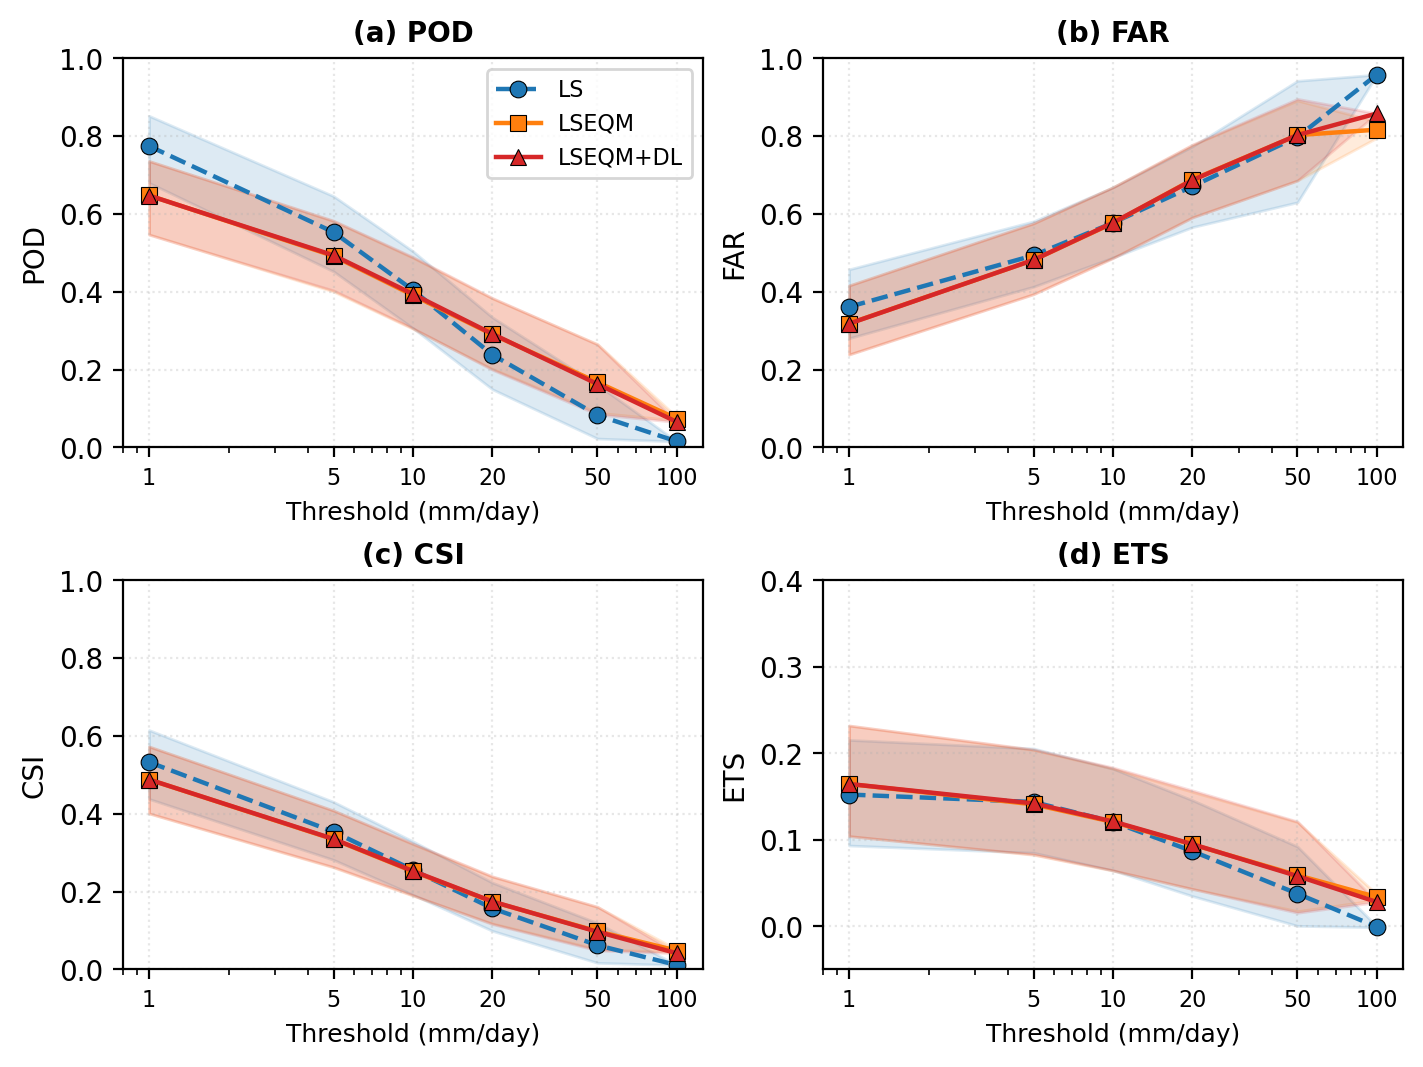
\includegraphics[width=\figFourTwoWidth\textwidth]{fig_thesis_04_multi_threshold.png}
\caption[Threshold-stratified verification at the $172$ BMKG station locations]{Detection skill as a function of daily rainfall threshold at the $172$ BMKG
station locations\label{fig:threshold-skill}}
\end{figure}


% ============================================================
\section{Pearson Correlation Across Stages}\label{sec:results-correlation}
% ============================================================

Section~\ref{sec:results-intercomparison} established, against the
independent BMKG stations and at both date labels, that the
correction does not lift the daily correlation. This section
reports the same result against the in-sample CPC-UNI target, so
the finding holds against both references.

One metric does not move across the three corrected stages. The Pearson
correlation between paired daily satellite and CPC-UNI values,
computed at each pixel and pooled across the dekad, is $0.343$
for LS, $0.345$ for LSEQM, and $0.348$ for LSEQM+DL. The total
shift across stages is approximately $+0.005$, well within the
single-pixel sampling uncertainty of $\pm 0.06$ implied by the
Fisher $z$-transform standard error at $n = 250$
\citep{ref:wilks2020}.

Figure~\ref{fig:paradox} states the central observation of this
chapter in four panels. Pearson $r$, root mean square error
(RMSE), and Nash-Sutcliffe efficiency (NSE)
\citep{ref:nashsutcliffe1970} are temporal-skill diagnostics
measured here against the in-sample CPC-UNI target, and they do
not improve across the three corrected stages: $r$ stays near
$0.35$ across all three, RMSE rises from $13.1$ to $14.1$~mm/day
because the correction widens spread without re-aligning timing,
and NSE moves from $-0.27$ to $-0.52$. The standard-deviation
ratio, an amplitude diagnostic measured against the independent
BMKG gauges, moves from $0.71$ to $1.00$ across the same stages.
The amplitude is corrected to the validation target, yet the
timing does not improve even against the reference the correction
was fitted to.

\begin{figure}[H]
\centering
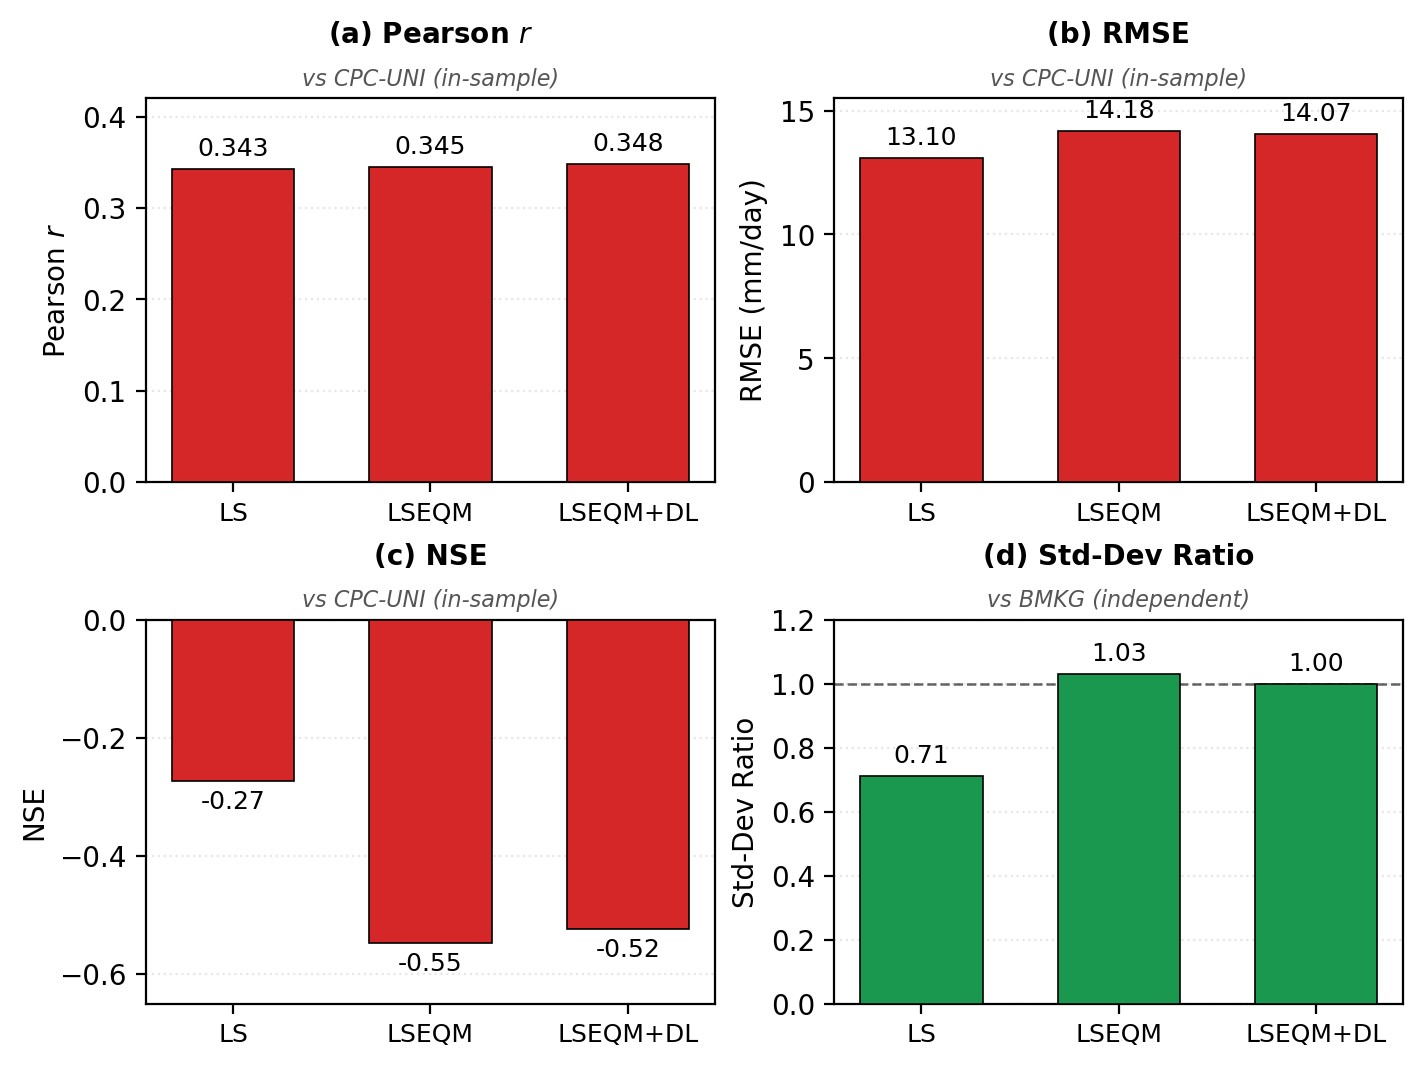
\includegraphics[width=\figFourThreeWidth\textwidth]{fig_thesis_04_paradox.png}
\caption[What does and does not improve under marginal bias correction]{What does and does not improve under marginal bias
correction, with the temporal-skill panels scored against CPC-UNI and the amplitude panel against BMKG.\label{fig:paradox}}
\end{figure}

The contrast is not a verification quirk; it is what the
framework should do given how each metric is built. The SDR
depends only on the marginal variance of the two series and is
therefore moved directly by the EQM stage acting on the daily
distribution. Pearson $r$, RMSE, and NSE depend on the
day-by-day pairing of satellite and gauge values and inherit
whatever timing offset the satellite product carries from its
half-hourly inputs and the daily aggregation window. The
marginal correction has no mechanism to shift a value from one
day to its neighbour, so by construction it cannot lift the
three temporal-skill metrics. The visual asymmetry between the
amplitude-pillar improvement and the temporal-skill diagnostics
is the central observation of this thesis;
Section~\ref{sec:discussion-bound} develops the theoretical
basis for the bound.

The empirical value $r \approx 0.348$ is of the
order reported for daily IMERG over the
Indonesian Maritime Continent \citep{ref:ramadhan2022ts}, and well
below the median near $0.75$ that the same product reaches against
the far denser Chinese gauge analysis
\citep[Fig.~3]{ref:tang2020}. That gap is not left unexplained:
Section~\ref{sec:results-window} shows most of it is a
calendar-window effect rather than a retrieval one.

The single figure $r \approx 0.35$ is the spatial mean of a broad
per-pixel distribution. Table~\ref{tab:cpc-corr-dist} and
Figure~\ref{fig:cpc-corr-dist} characterise the daily correlation
against CPC-UNI across the full $0.1^{\circ}$ domain: over the
$19{,}393$ land pixels it spans $0.08$ to $0.68$, with a median of
$0.35$ and a pooled value of $0.36$.

The correlation is markedly
higher where the CPC-UNI gauge network is dense: at the $169$ cells
that host at least one of the $180$ BMKG stations the median and the
pooled value are both $0.51$, against $0.35$ and $0.36$
domain-wide. The gridded
reference is better constrained where the gauges cluster. At every aggregation the
value is flat across the three corrected stages (whole-domain
pooled $0.350$, $0.360$, and $0.363$), so the near-flat behaviour
of $r$ is a property of the whole field, not of a particular sample
of points. All of these are measured against CPC-UNI, the in-sample
calibration target; the independent, out-of-sample comparison
against the BMKG point gauges is lower and is decomposed in
Section~\ref{sec:results-window}, where the day-by-day pairing
against the station observations proves to be dominated by the
calendar-window mismatch rather than by retrieval skill.

\begin{table}[H]
\centering
\caption[Daily correlation against CPC-UNI across the domain]{Daily Pearson $r$ of the corrected product against CPC-UNI across the domain over the full 2001 to 2025 record, by correction stage\label{tab:cpc-corr-dist}}
\begingroup\small
\begin{tabular*}{\textwidth}{@{\extracolsep{\fill}}lccccc@{\hskip 1.4em}c@{}}
\toprule
& \multicolumn{5}{c}{Whole coverage ($19{,}393$ pixels)} & Gauge cells \\
\cmidrule(lr){2-6}
Stage & Min & Mean & Median & Max & Pooled & Pooled \\
\midrule
LS       & $0.092$ & $0.351$ & $0.341$ & $0.670$ & $0.350$ & $0.503$ \\
LSEQM    & $0.082$ & $0.352$ & $0.344$ & $0.673$ & $0.360$ & $0.508$ \\
LSEQM+DL & $0.082$ & $0.355$ & $0.346$ & $0.677$ & $0.363$ & $0.513$ \\
\bottomrule
\end{tabular*}
\endgroup
\end{table}

Figure~\ref{fig:cpc-corr-dist} renders the same whole-coverage
distribution as a density and overlays the gauge-dense cells. The
domain forms a single broad mode centred near $0.35$, while the
gauge-dense cells sit as a distinct, right-shifted population
centred near $0.51$, so the density effect is visible directly
rather than only through the pooled summary.

\begin{figure}[H]
\centering
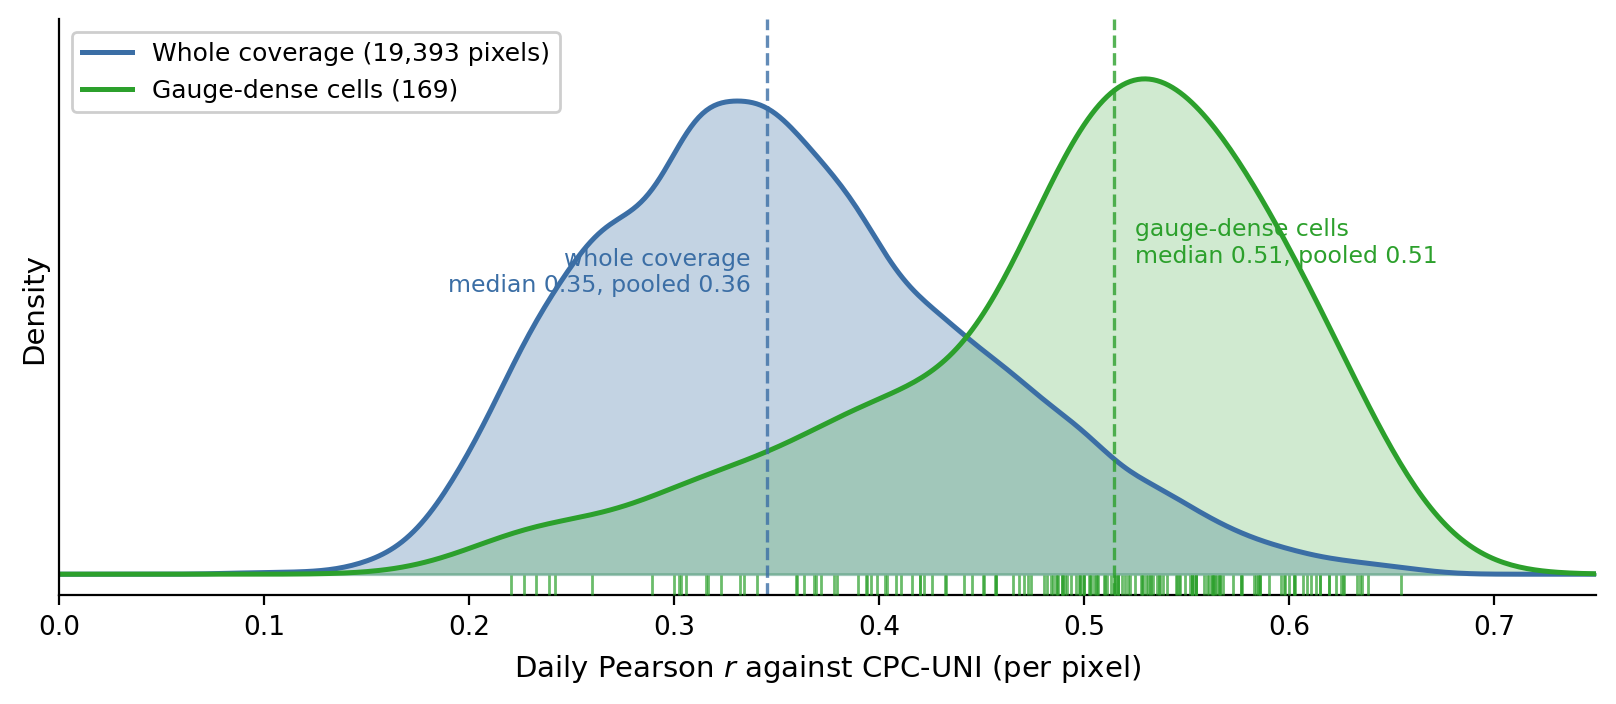
\includegraphics[width=0.98\textwidth]{fig_thesis_04_cpc_corr_dist.png}
\caption[Spatial distribution of the CPC-UNI daily correlation]{Per-pixel daily Pearson $r$ of the LSEQM+DL product against CPC-UNI: the whole-coverage field against the gauge-dense cells\label{fig:cpc-corr-dist}}
\end{figure}


% ============================================================
\section{Temporal Alignment and the Optimal Aggregation
Window}\label{sec:results-window}
% ============================================================

The near-flat correlation of
Section~\ref{sec:results-correlation} raises a question the stage
comparison cannot answer: how much of the absolute ceiling is set
by the retrieval timing, and how much by the calendar window used
to label each daily total. The daily IMERG-L archive accumulates
over the Coordinated Universal Time (UTC) day, whereas the BMKG
stations report under the morning-observation convention, a
24-hour total ending near $07{:}00$ local time. To separate the two
components, the half-hourly IMERG-L source is re-aggregated into
24-hour windows starting at every integer-hour offset
$h \in [-48, +48]$ from $00{:}00$~UTC and correlated against the
BMKG daily totals (Section~\ref{sec:methods-window}). The
diagnostic operates on the raw retrieval rather than the corrected
product. The diagnostic pools the $178$ of the $180$
BMKG stations that carry valid half-hourly coverage, a different
subset from the $172$ stations used for the dekadal
correction-metric validation.

Figure~\ref{fig:window-era} reports the result over the GPM era,
$2015$ to $2021$. The pooled correlation rises from $r = 0.20$ at
$h = 0$, the UTC-day alignment the daily archive uses, to
$r = 0.57$ at $h = -23$, the window that matches the local-day
gauge convention. This UTC-day value of $0.20$ is lower than the
dekad-sliced CPC-UNI value of $r \approx 0.35$
(Section~\ref{sec:results-correlation}) for two reasons: the full
record blends the GPM era with the earlier, timing-imprecise era,
and the window diagnostic pairs against the independent BMKG gauges
rather than the CPC-UNI reference used in
Section~\ref{sec:results-correlation}. Each contributes about
$0.10$, so neither alone accounts for the difference.

The recovery is
conditional on the satellite era. Before the full GPM
constellation, the years through $2013$, whose IMERG inputs derive
from the sparser TRMM-era sensor set, re-windowing does not lift
the correlation: it stays near $r = 0.36$ at every offset and the
peak offset wanders without a stable value. The window-matched
recovery appears only once the half-hourly field resolves the
diurnal cycle, a transition the per-year trace places at the
$2014$ to $2015$ boundary.

\begin{figure}[H]
\centering
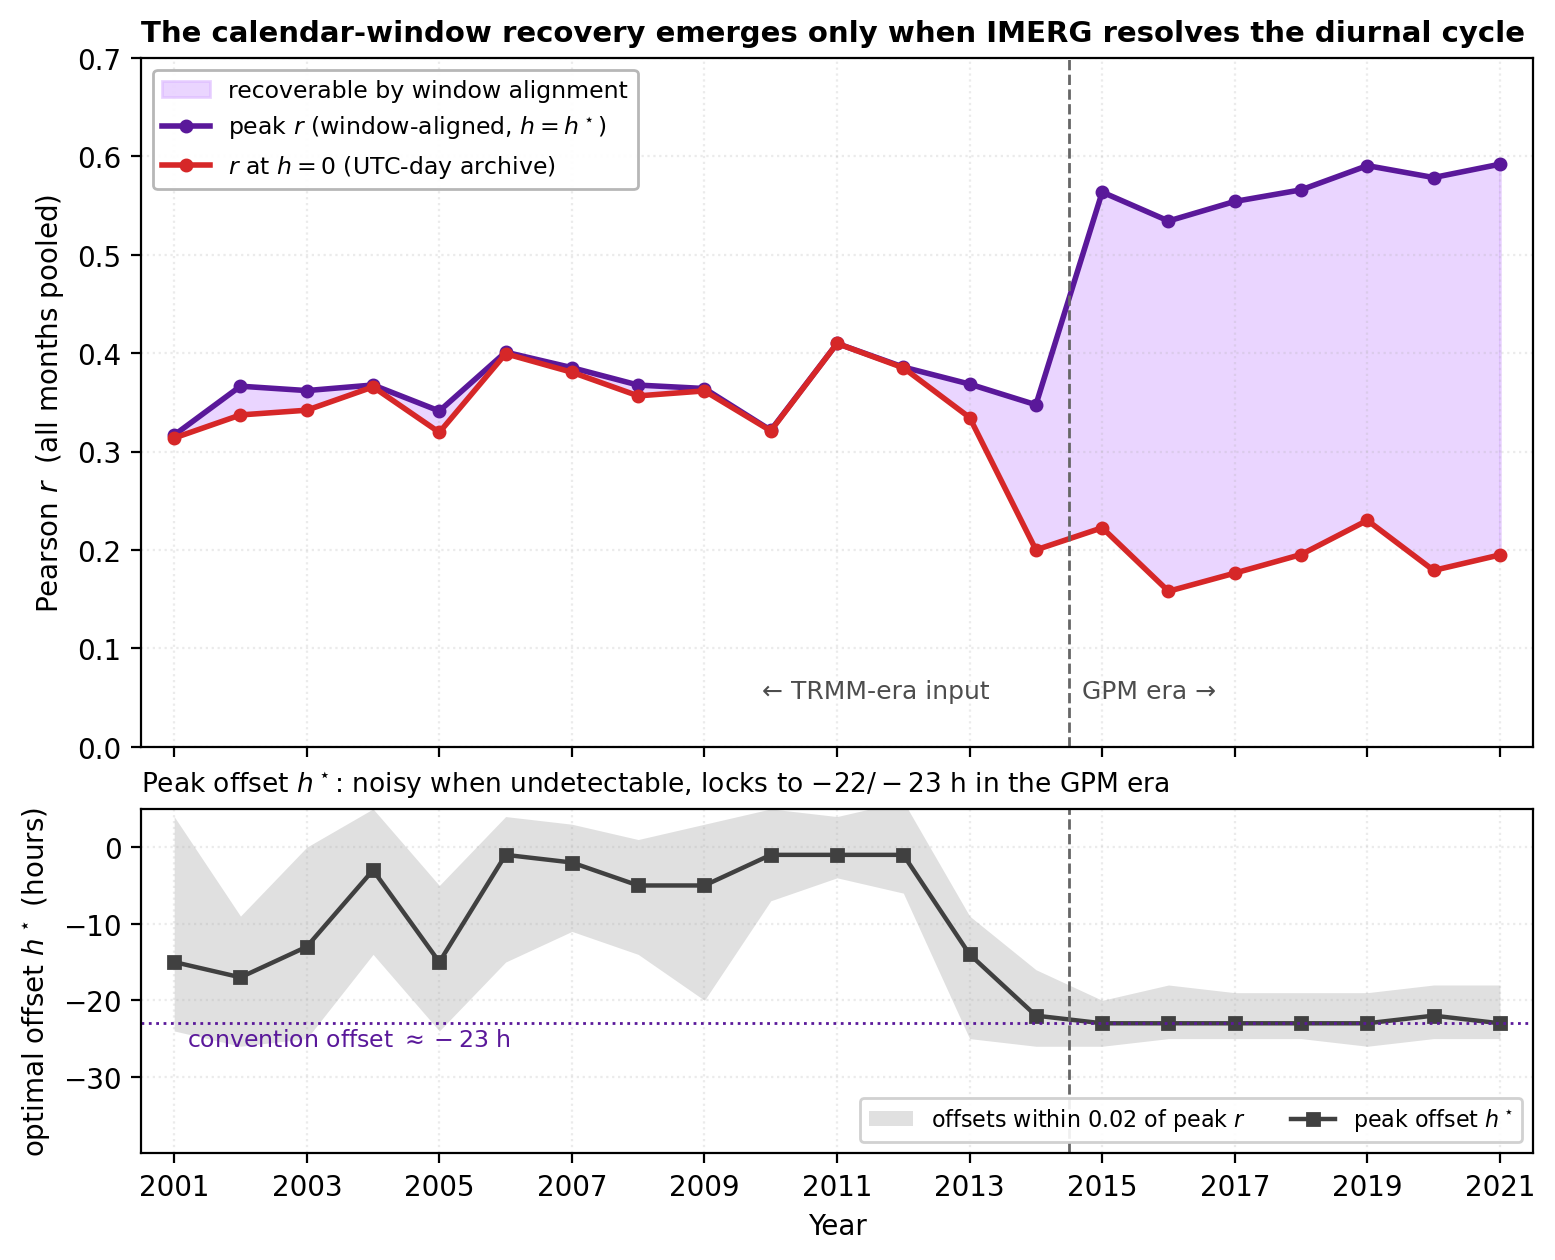
\includegraphics[width=\figFourNineWidth\textwidth]{fig_thesis_04_window_era.png}
\caption[Window-offset correlation recovery by satellite era]{Per-year
Pearson~$r$ at the UTC-day window ($h = 0$) and at each year's
best-matched window, with the peak offset~$h^{\star}$ below.\label{fig:window-era}}
\end{figure}

The optimal offset is stable across the seasonal cycle. Across all
twelve three-month running seasons the pooled peak sits at
$h = -23$~h in every timezone band
(Appendix~\ref{app:window}~Figure~\ref{fig:window-seasonal}), and
the optimum does not
migrate between the wet and dry monsoon phases.

The offset is equally stable across space. The per-station peak
offset has a median of $-23$~h, an interquartile range of
$[-23, -21]$~h, and no systematic longitudinal organisation across
the WIB, WITA, and WIT timezone bands
(Appendix~\ref{app:window}~Figure~\ref{fig:window-map}). The recovered per-station
correlation has a median of $0.56$, an interquartile range of
$0.51$ to $0.62$, and a maximum near $0.78$; taking the same
per-station median within each timezone band gives $0.55$ for WIB
and WITA and $0.61$ for WIT. The offset is therefore a property of the gauge
reporting convention shared across the network, not a local effect.

The window choice governs daily skill but not monthly skill.
Aggregating the same daily totals to monthly sums and validating
against the BMKG monthly totals returns a correlation near $0.80$
whether the daily windows are UTC-aligned or gauge-matched
(Table~\ref{tab:window-monthly}): a one-day window shift only
redistributes one or two days across each month boundary, so it is
invisible at the monthly scale. The same product that scores
$r = 0.20$ against the daily gauges at the UTC-day alignment scores
$r = 0.80$ against the monthly gauges, which places the daily
ceiling in the timing of the day-by-day pairing rather than in the
amount of rainfall the product captures.

\begin{table}[H]
\centering
\caption[Daily versus monthly correlation under two aggregation windows]{Daily
and monthly Pearson~$r$ under the UTC-day and gauge-matched windows
(GPM era; $n = 5{,}338$ station-months)}
\label{tab:window-monthly}
\begin{tabular*}{\textwidth}{@{\extracolsep{\fill}}lcc@{}}
\toprule
Aggregation window & Daily $r$ & Monthly $r$ \\
\midrule
UTC day ($h = 0$)        & $0.20$ & $0.80$ \\
Gauge-matched ($h = -23$) & $0.57$ & $0.81$ \\
\bottomrule
\end{tabular*}
\end{table}

These results localise the near-flat correlation of
Section~\ref{sec:results-correlation}: the larger part of the gap
between the UTC-day value and the gauge-matched value is a
calendar-window component, recoverable by re-aggregating the
archive over a window matched to the gauge convention, and the
remainder is a residual retrieval-skill component that no window
choice removes. The four-pillar value, distribution, extreme, and
detection scores are functions of the marginal distribution and of
categorical events, and are unchanged by the window observation.
Section~\ref{sec:discussion-subdaily} develops the interpretation:
why the recovery is confined to the GPM era, and what the
re-aggregation implies operationally.
Appendix~\ref{app:window} carries the supporting diagnostics for
this section, including the per-offset curves behind the summary
values reported here.


% ============================================================
\section{Spatial Skill Distribution}\label{sec:results-cqi}
% ============================================================

The headline numbers in Section~\ref{sec:results-headline} pool
across the full Indonesian domain and so average over the
regional heterogeneity of Java-Sumatra-Bali gauge density against
the sparse network in Maluku and Papua. The Composite Quality
Index (CQI) defined in Section~\ref{sec:methods-metrics}
collapses the per-pixel performance across the three sub-scores
(Basic Statistical Quality sub-score (BSQS), Distribution Quality sub-score (DQS), Temporal Quality sub-score (TQS)) and lets the spatial distribution of skill be
read as a single map. Figure~\ref{fig:cqi-spatial} shows the
CQI for the three correction stages, computed per pixel against
the in-sample CPC-UNI target.

\begin{figure}[H]
\centering
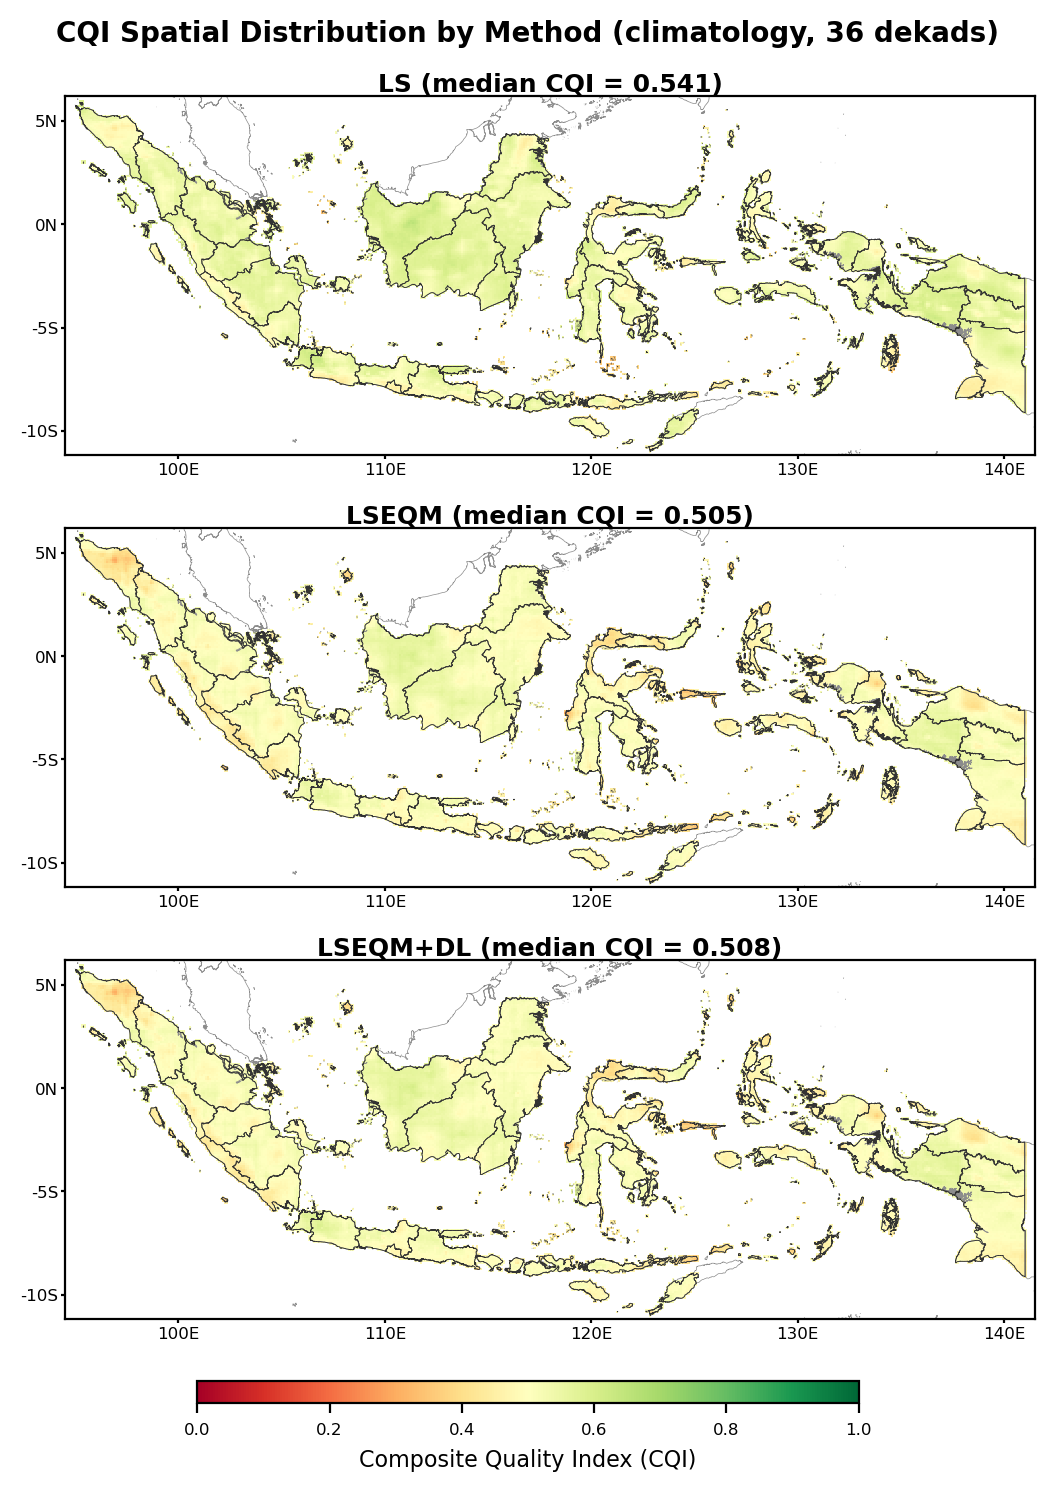
\includegraphics[width=\figFourFourWidth\textwidth]{fig_thesis_04_cqi_spatial.png}
\caption[CQI maps for the three correction stages]{CQI maps for (top) Linear Scaling, (middle) LSEQM, and (bottom) LSEQM+DL, computed
pixel-wise against CPC-UNI and averaged across all $36$ dekadal
windows.\label{fig:cqi-spatial}}
\end{figure}

The map view makes the regional heterogeneity visible: high
quality across Java and southern Sumatra where the gauge network
is dense, progressively lower quality eastward into Maluku and
Papua where the reference dataset itself is poorly constrained.
The differences between LSEQM and LSEQM+DL are concentrated in
the densely gauged regions, where the CNN refinement contributes
through the station-density-aware blending of
Section~\ref{sec:methods-blending}; in sparsely gauged regions
the framework reverts toward the LSEQM result by design, so the
LSEQM and LSEQM+DL maps are nearly indistinguishable there.

Appendix~\ref{app:atlas}~Figure~\ref{fig:cqi-improvement} isolates the LSEQM+DL
contribution by mapping the per-pixel CQI change from LSEQM to
LSEQM+DL (panel~a) and the LSEQM+DL CQI itself (panel~b) against
the four operational quality tiers (Poor $<0.4$, Fair $0.4$ to $0.6$,
Good $0.6$ to $0.8$, Excellent $\geq 0.8$). The change from the CNN
step is small and never negative. It stays within $\pm 0.01$ CQI
across most of the domain and rises to modest positive values over
the densely gauged western islands where the refinement is most
active (mean $+0.003$, exceeding $+0.01$ over $3.8\%$ of pixels and
falling below $-0.01$ over none).

The CQI map places the product in
the Fair band ($0.40$ to $0.60$) across $98.5\%$ of the land mass
(mean $0.503$), with a west-east gradient that tracks gauge
density. The product sits higher within the Fair band over Java, Sumatra, and the
well-observed interiors, and drops into the Poor tier over the
$1.5\%$ of pixels in the most sparsely gauged east. It does not
reach the Good or Excellent tier anywhere; against the sparse CPC
reference the attainable CQI is bounded within the Fair band,
consistent with the confidence mask reverting toward LSEQM where
stations are sparse.


The spatial pattern carries an important operational reading.
The headline LSEQM+DL numbers reported in
Table~\ref{tab:headline} apply with full strength in the
densely gauged west; in the eastern sparsely gauged regions the
relevant performance baseline is the LSEQM column rather than
the LSEQM+DL column, because the blending formula in
Section~\ref{sec:methods-blending} suppresses the CNN
contribution there. Users in Java, Sumatra, and Bali receive
the full benefit of the four-stage pipeline; users in Maluku
and Papua receive the LSEQM result with a thin and locally
variable CNN residual on top. The framework therefore does not
over-claim accuracy in regions where the reference dataset
itself cannot support refinement, which is the operational
expression of the design choice to make the CNN density-aware
rather than uniform. Pillar-by-pillar climatological metric maps
for each correction stage, on the same Indonesian domain, are in
Appendix~\ref{app:atlas}~Figure~\ref{fig:atlas-pillars}.


% ============================================================
\section{Per-Station Taylor Diagram Analysis}\label{sec:results-taylor}
% ============================================================

The aggregate pattern reported in
Sections~\ref{sec:results-headline} and
\ref{sec:results-correlation} can be cross-checked at the level
of individual BMKG stations using a Taylor diagram, which plots
each station as a point whose angular position encodes the
Pearson correlation against the gauge series and whose radial
position encodes the standard deviation ratio relative to the
gauge target. Figure~\ref{fig:taylor-station} shows the
station-level diagram broken out by season: the wet season
(November to April) and the dry season (May to October), which
are the operationally meaningful periods for Indonesian
agriculture and water management.

\begin{figure}[H]
\centering
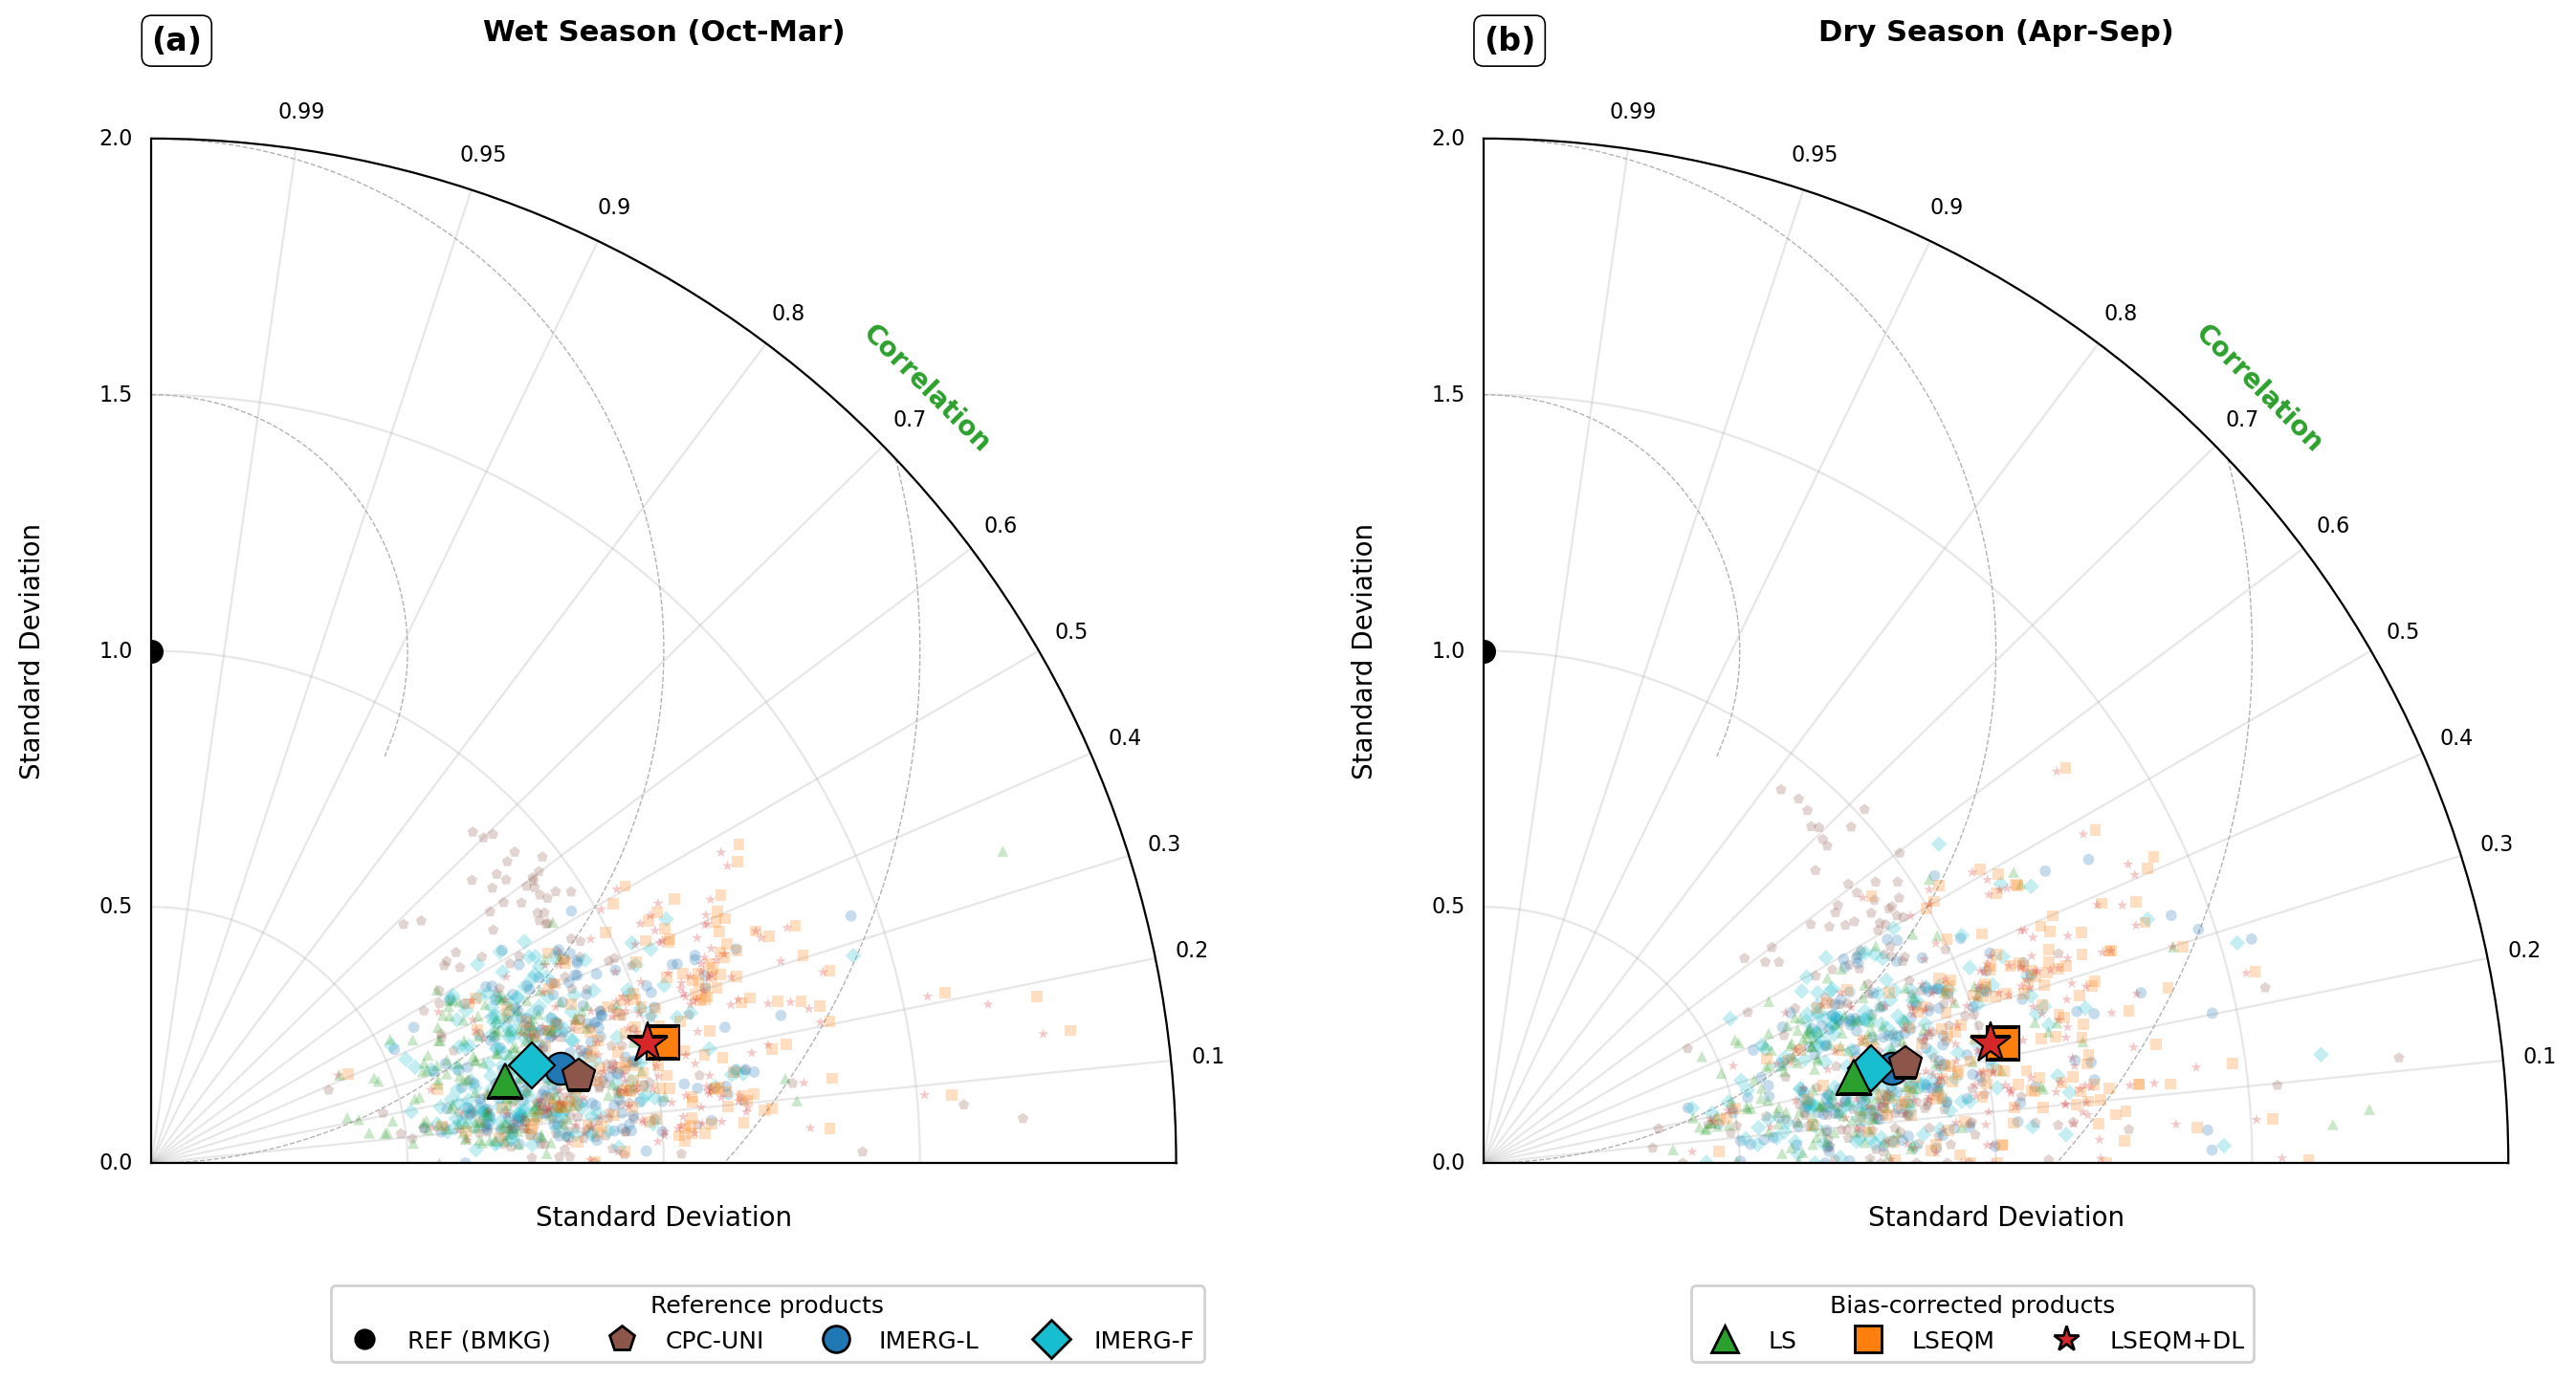
\includegraphics[width=\figFourSixWidth\textwidth]{fig_thesis_04_taylor_by_station.png}
\caption[Station-level Taylor diagram of BMKG validation by season]{Station-level Taylor diagram of BMKG validation by
season\label{fig:taylor-station}}
\end{figure}

The Taylor diagram resolves the headline pattern across
individual stations: the three method symbols cluster at the
same angular position (correlation) while their radial positions
(standard deviation) differ substantially, with LSEQM and
LSEQM+DL sitting close to the reference radius and LS sitting
short. The pattern is conserved across both seasons, so the
flat-correlation observation is not driven by either the
convective wet season or the gauge-sparse dry season alone but
holds station-by-station and season-by-season across the
archipelago. This per-station visual evidence anticipates the
theoretical argument in Section~\ref{sec:discussion-bound}: the
correlation stays pinned close to the underlying retrieval timing,
which is a property of the satellite product at each pixel and
each day, and is not lifted by the marginal correction at any
of the $178$ stations carrying a valid correlation in this
diagnostic.
Appendix~\ref{app:atlas}~Figure~\ref{fig:atlas-stations}
places the validation stations directly on dekadal-mean
precipitation maps of the four products as a visual spatial
agreement check, and Appendix~\ref{app:stations} reports the
per-station statistics behind this diagram for a selected subset
of the network.


% ============================================================
\section{Temporal Stability Across Dekads}\label{sec:results-temporal}
% ============================================================

The dekadal pooling design of
Section~\ref{sec:methods-validation} aggregates each of the
$36$ dekadal windows into a single metric value, which masks
the within-year variability that drives operational use across
the Indonesian wet and dry seasons. This section recovers the
monthly view by re-aggregating the dekadal metrics to a
calendar-month axis and reports four representative metrics
(SDR, RMSE, KS $p$-value, CSI) across the three correction
stages, in Figure~\ref{fig:temporal-stability}. These are the
per-pixel metrics measured against the
in-sample CPC-UNI target, not the per-station BMKG values of
Section~\ref{sec:results-headline}.

\begin{figure}[H]
\centering
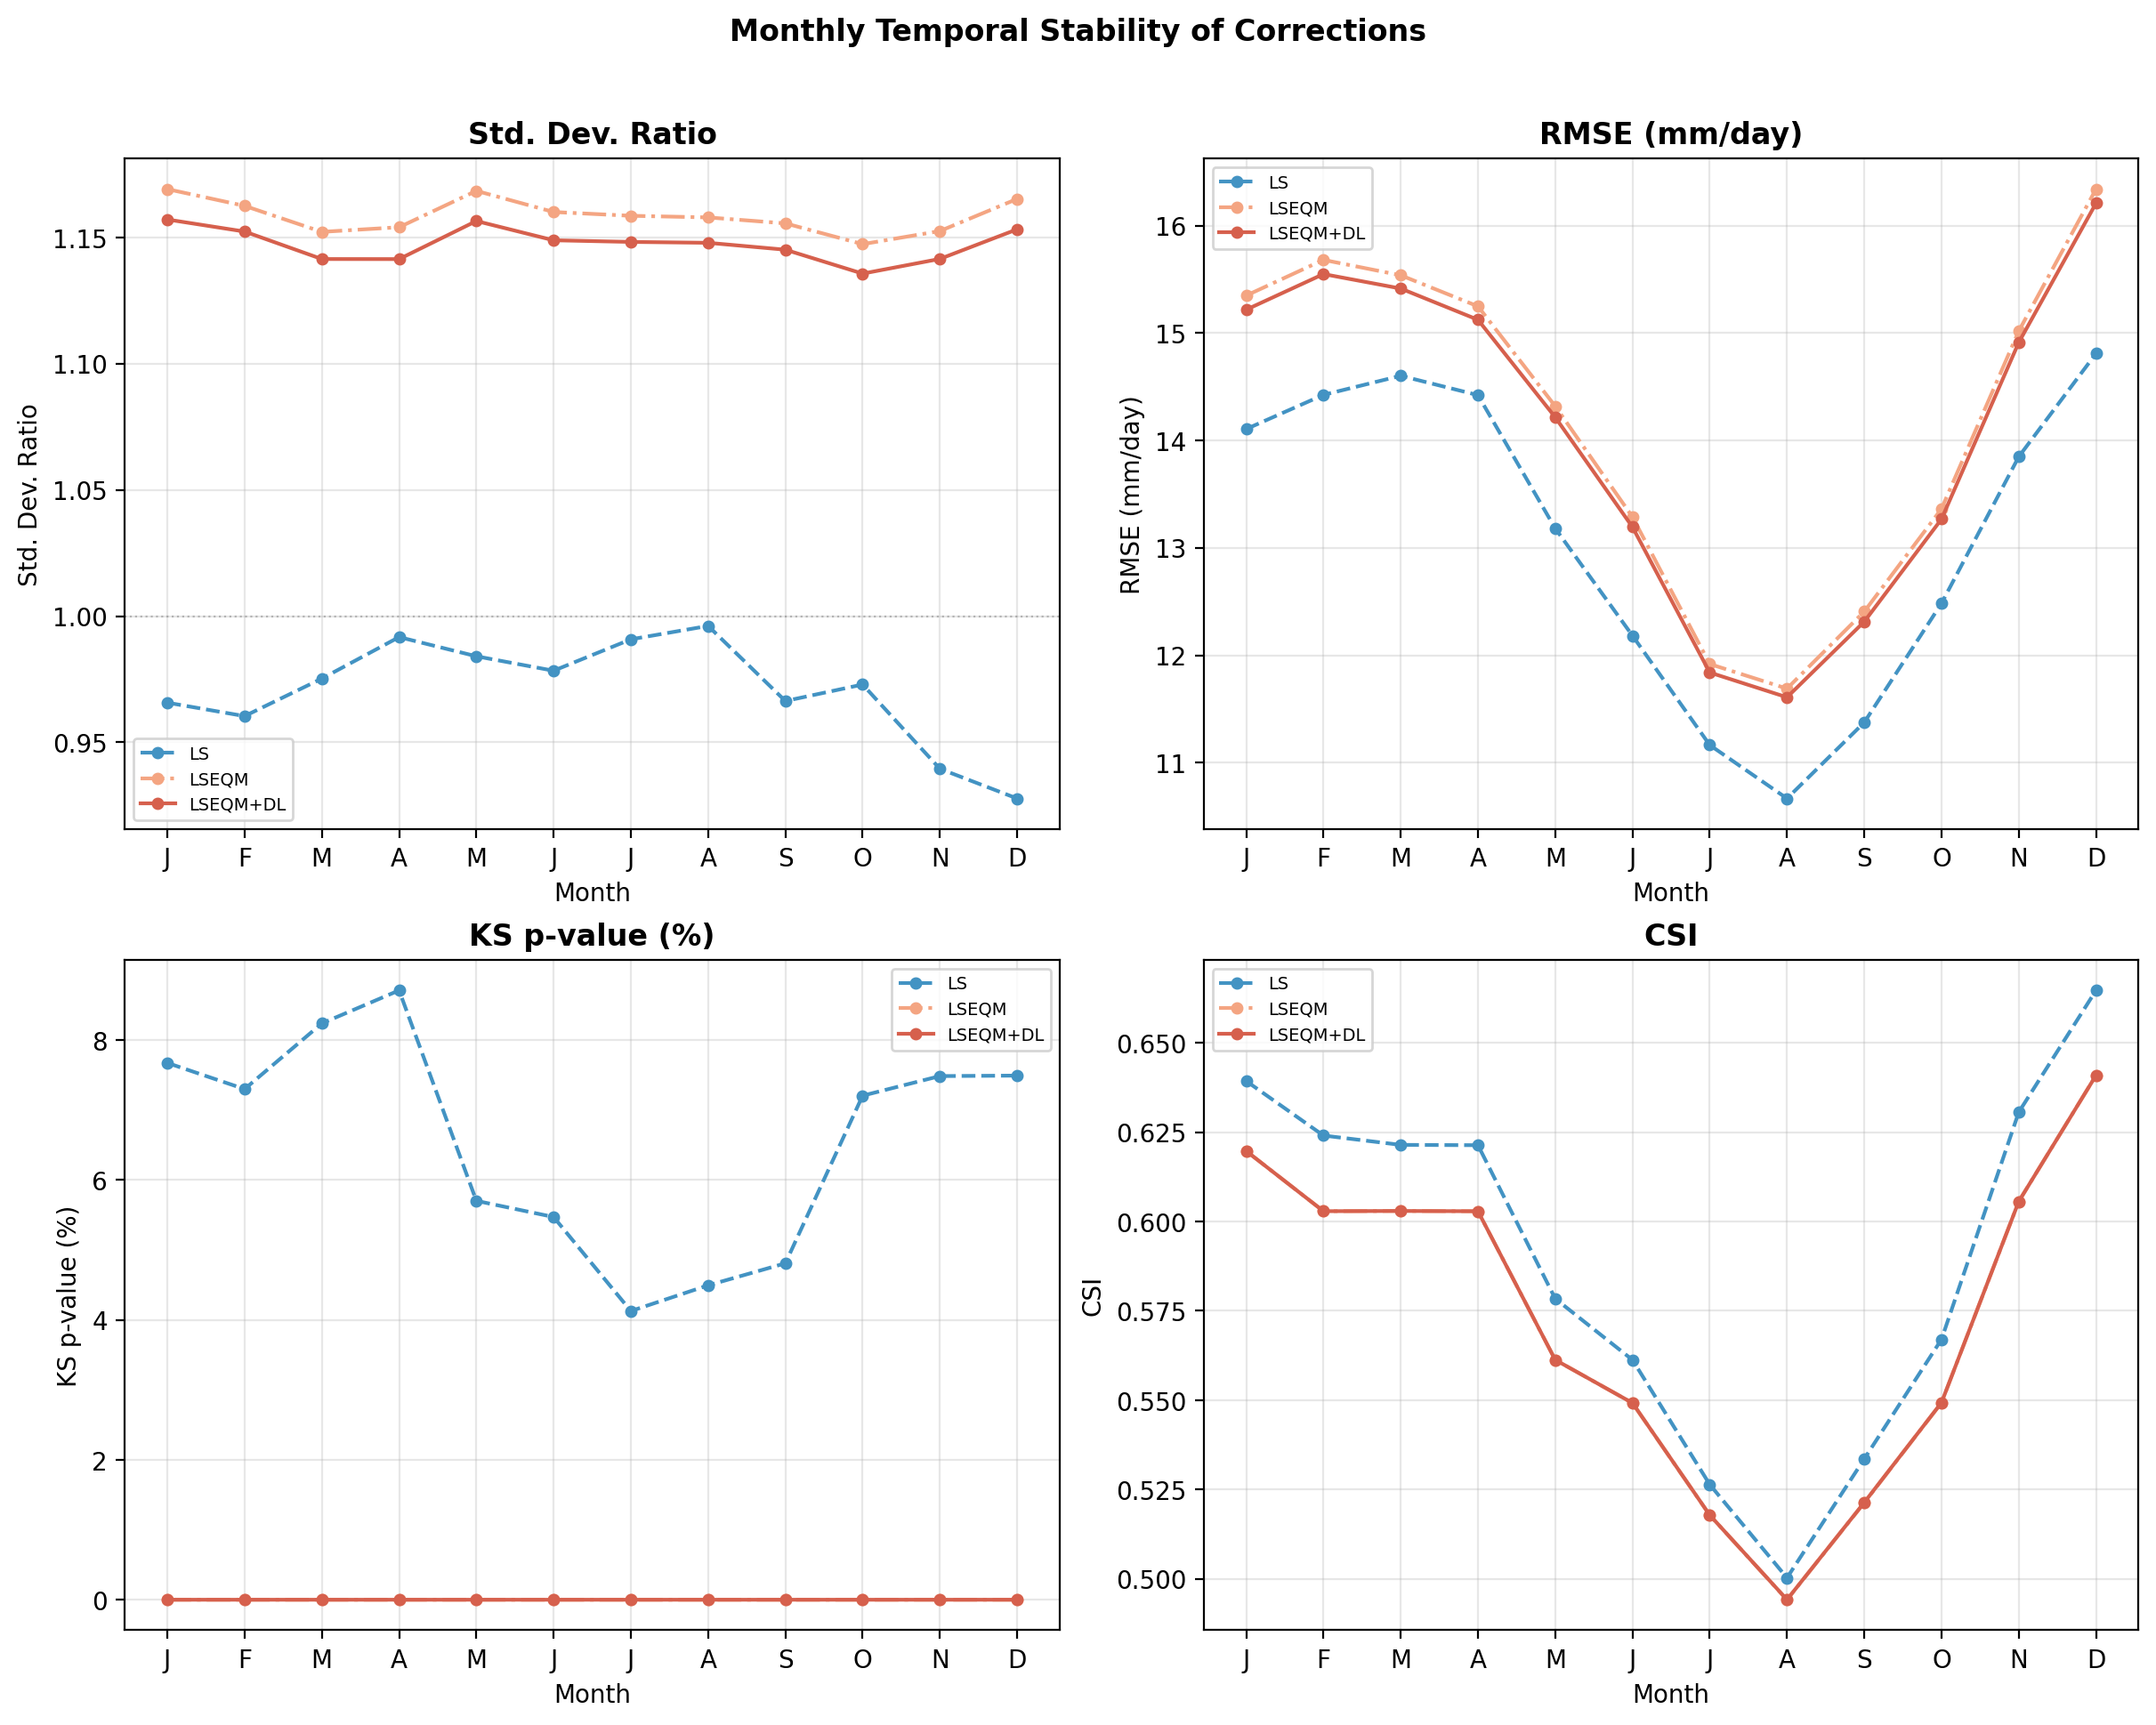
\includegraphics[width=\figFourSevenWidth\textwidth]{fig_thesis_04_temporal_stability.png}
\caption[Monthly temporal stability of four representative metrics across the three correction stages]{Monthly temporal stability of four representative
metrics across the three correction stages, measured per pixel against CPC-UNI\label{fig:temporal-stability}}
\end{figure}

The SDR stays near $1.0$ for LSEQM and LSEQM+DL across all
months, indicating that the spread correction is stable across
the seasonal cycle and does not require season-specific
calibration. RMSE rises during the peak wet season (December
to February) when absolute precipitation magnitudes are
largest, which is a property of any squared-error metric on a
distribution with a wet-season fat tail rather than a
correction artefact. The KS $p$-value remains above the
$5\%$ acceptance threshold for both LSEQM and LSEQM+DL across
all months except the deepest wet-season months, where the
high counts of heavy-rain days reduce the test power. CSI
shows a modest seasonal cycle, but the ordering seen in the
per-pixel panel, with LS above LSEQM and LSEQM+DL at the
$1$~mm wet-day threshold at which the gridded CSI is computed,
is conserved month-by-month. The threshold-dependent reversal
of Section~\ref{sec:results-threshold} is a BMKG station result
and is not visible here.
A daily-scale spatial example of the day-to-day variation across
three contrasting days in the same dekad is in
Appendix~\ref{app:atlas}~Figure~\ref{fig:atlas-threedays}.

The monthly view confirms that the per-pixel medians in
Table~\ref{tab:headline-cpc} are not driven by a small subset of
dekads. The pattern of stage-wise attribution is consistent across
the seasonal cycle: each stage moves the metrics matched to
its design dimension in every month, and the temporal-skill
ceiling on Pearson $r$ persists in every month. The dekadal
pooling design is therefore a legitimate way to aggregate
results across years for the comparison framework of
Section~\ref{sec:results-headline}, because the underlying
pattern does not change qualitatively from month to month.


% ============================================================
\section{Sensitivity Analyses}\label{sec:results-sensitivity}
% ============================================================

Three parameters in the pipeline were set by domain reasoning
rather than by a formal cross-validated search: the CNN blending
weight $\alpha = 0.70$, the GPD threshold at the $80$th wet-day
percentile, and the station-density saturation count
$c_{\text{sat}} = 2$. This section states the expected
direction of effect of each, drawn from the design reasoning in
Chapter~\ref{chap:methods}, then reports a parameter sweep over
the Bali reproducibility subdomain
(Section~\ref{sec:results-reproducibility}) that tests those
predictions empirically. The subdomain is used because each of the
fifteen settings requires a complete correction and
metric-evaluation run, including per-dekad CNN training: the sweep
is tractable on the $126$-pixel Bali grid, but the per-pixel stages
scale with the pixel count, and for the $19{,}395$ land
pixels of the full domain a fifteen-run national sweep is impractical
on commodity hardware. A full-domain sweep with a strict temporal
hold-out remains future work.

The blending weight $\alpha$ sets the maximum CNN contribution
in fully gauge-supported pixels through
Equation~\eqref{eq:alpha-eff}: a larger $\alpha$ moves the
blend toward pure LSEQM and reduces the CNN influence, while a
smaller $\alpha$ admits more of the learned residual. The
operating value $0.70$ caps the CNN at a $30\%$ contribution
where confidence is full, a deliberately conservative setting
that limits the spatial refinement to a correction rather than
a replacement.

The GPD threshold percentile trades sample size
against tail purity. Lowering it from the $80$th toward the
$70$th admits more exceedances and stabilises the maximum-likelihood
fit, but conflates the extreme regime with moderate rain that the
Gamma EQM already handles. Raising it toward the $90$th
sharpens the extreme regime at the cost of falling below the
exceedance count needed for a stable fit in dry pixels
(Section~\ref{sec:methods-gpd}).

The saturation count
$c_{\text{sat}}$ sets how many contributing gauges per CPC cell
are needed for full confidence. A larger value is more
conservative and suppresses the CNN across more of the domain,
while a smaller value admits the CNN more widely. The value $2$
was chosen after an initial setting of $3$ was found to suppress
the CNN almost everywhere outside Java.

The sweep varies each parameter through five values while
holding the other two at their operating defaults, runs the full
LSEQM+DL pipeline end-to-end on the Bali subdomain for all $36$
dekadal windows of the $2001$ to $2025$ record, and pools the
resulting per-pixel metrics.
Table~\ref{tab:sensitivity-bali} reports the fifteen settings,
with the operating default of each parameter shown in bold and
the per-pixel metrics given as $r$ (Pearson correlation), RB
(relative bias, \%), SDR (standard-deviation ratio), RMSE (root
mean square error, mm/day), and NSE (Nash-Sutcliffe efficiency).

\begin{table}[H]
\centering
\caption[Bali sensitivity sweep over the three configuration parameters]{Bali sensitivity sweep over the three configuration
parameters identified in Chapter~\ref{chap:methods}, reported per pixel against CPC-UNI at the native window over the $2001$ to $2025$ record\label{tab:sensitivity-bali}}
\begingroup\small
\begin{tabular*}{\textwidth}{@{\extracolsep{\fill}}lcccccc@{}}
\toprule
Parameter & Value & $r$ & RB (\%) & SDR & RMSE & NSE \\
\midrule
\multicolumn{7}{l}{\textit{Blending weight} $\alpha$} \\
$\alpha$ & $0.50$ & $0.344$ & $-14.5$ & $0.910$ & $5.88$ & $-0.40$ \\
         & $0.60$ & $0.343$ & $-14.9$ & $0.907$ & $5.89$ & $-0.40$ \\
         & $\mathbf{0.70}$ & $\mathbf{0.340}$ & $\mathbf{-15.0}$ & $\mathbf{0.905}$ & $\mathbf{5.89}$ & $\mathbf{-0.41}$ \\
         & $0.80$ & $0.336$ & $-15.2$ & $0.903$ & $5.90$ & $-0.41$ \\
         & $0.90$ & $0.332$ & $-15.5$ & $0.900$ & $5.91$ & $-0.41$ \\
\midrule
\multicolumn{7}{l}{\textit{GPD threshold percentile}} \\
Pctl     & $70$ & $0.345$ & $-13.0$ & $0.923$ & $5.96$ & $-0.42$ \\
         & $75$ & $0.342$ & $-13.7$ & $0.919$ & $5.96$ & $-0.41$ \\
         & $\mathbf{80}$ & $\mathbf{0.340}$ & $\mathbf{-15.0}$ & $\mathbf{0.905}$ & $\mathbf{5.89}$ & $\mathbf{-0.41}$ \\
         & $85$ & $0.337$ & $-16.2$ & $0.891$ & $5.82$ & $-0.40$ \\
         & $90$ & $0.335$ & $-18.0$ & $0.867$ & $5.72$ & $-0.39$ \\
\midrule
\multicolumn{7}{l}{\textit{Density saturation count} $c_{\text{sat}}$} \\
$c_{\text{sat}}$ & $1$ & $0.348$ & $-14.7$ & $0.911$ & $5.88$ & $-0.40$ \\
                 & $\mathbf{2}$ & $\mathbf{0.340}$ & $\mathbf{-15.0}$ & $\mathbf{0.905}$ & $\mathbf{5.89}$ & $\mathbf{-0.41}$ \\
                 & $3$ & $0.336$ & $-15.3$ & $0.903$ & $5.90$ & $-0.41$ \\
                 & $4$ & $0.334$ & $-15.3$ & $0.902$ & $5.90$ & $-0.41$ \\
                 & $5$ & $0.333$ & $-15.4$ & $0.901$ & $5.91$ & $-0.41$ \\
\bottomrule
\end{tabular*}
\endgroup
\end{table}

Three findings follow. First, every parameter produces a
monotone, locally smooth response across the explored range, and
none of the fifteen settings reverses the headline pattern of
Section~\ref{sec:results-headline} that LSEQM+DL moves value
adjustment, distribution alignment, and tail preservation toward
the gauge target.

Second, the Pearson correlation stays in the
narrow band $[0.332, 0.348]$ across all fifteen settings, a
spread of $0.016$. No setting shifts the daily correlation by
more than this amount, consistent with the interpretation of
Section~\ref{sec:results-correlation} that the daily correlation
is set by the timing skill of the raw retrieval rather than
by the choice of correction parameter \citep{ref:maraun2013}. This
flatness follows from the rank-preserving nature of the correction,
not from any property of the Bali subdomain, so it is a structural
result that holds wherever the pipeline is applied: the
correction-parameter insensitivity of the daily correlation is not
specific to Bali. The magnitudes of the distribution and bias
responses in Table~\ref{tab:sensitivity-bali}, by contrast, are
subdomain-specific and would differ in size over other regions, even
though their direction of effect follows the design reasoning above.

Third, the GPD threshold percentile dominates the dispersion:
raising the percentile from the $70$th to the $90$th narrows
the corrected distribution (SDR falls from $0.923$ to $0.867$)
and shifts relative bias more negative (from $-13.0\%$ to
$-18.0\%$), while RMSE falls modestly (from $5.96$ to
$5.72$~mm/day). The blending weight and the saturation count
each move bias by no more than one percentage point and SDR by
less than $0.012$ across their full sweep range. The operating choice
therefore sits inside a flat region for two of the three
parameters, with the GPD threshold the single setting at which a
downstream user would most need to revisit the trade-off.

The sweep script that produced Table~\ref{tab:sensitivity-bali}
accompanies the released code, so the table can be regenerated
without modifying the pipeline.


% ============================================================
\section{Reproducibility Evaluation}\label{sec:results-reproducibility}
% ============================================================

The reproducibility design described in
Section~\ref{sec:methods-reproducibility} is only meaningful if
the pipeline runs end-to-end on commodity hardware. To
demonstrate this, the correction-to-visualisation notebooks were
re-executed on a free-tier Google Colab instance for a
province-scale subdomain of Bali (a $9 \times 14$ pixel grid at
$0.1^{\circ}$, spanning $114.4$ to $115.7^{\circ}$E and $-8.85$
to $-8.05^{\circ}$N), processing all $36$ dekadal windows of the
$2001$ to $2025$ record. Bali was chosen because it is small
enough to run within the free-tier session limits while
exercising every stage of the pipeline.
Appendix~\ref{app:repro}~Figure~\ref{fig:bali-coverage} shows the
subdomain and its data coverage.

Table~\ref{tab:colab-runtime} reports the measured wall-clock
time for the all-dekad batch in each notebook, recorded from the
Colab cell-execution metadata. The correction-to-visualisation
sequence over the
Bali subdomain completed in $72.1$ minutes on a standard Central
Processing Unit (CPU) runtime with no hardware accelerator, well
within a single
free-tier session. The figure covers notebooks $02$ to $06$ and
excludes the two preparatory notebooks, whose timing is dominated
by the domain extent requested and by network throughput and so is
not reproducible.

This $72.1$-minute figure is the cost of all
$36$ dekads for the $126$-pixel Bali grid, not of the full
Indonesian domain, which contains on the order of $10^{4}$ to
$10^{5}$ land pixels and would scale roughly in proportion to the
pixel count for the per-pixel stages. It demonstrates that the
pipeline runs on free-tier infrastructure for a self-contained
region; it is not a timing estimate for a national run. Within
that run, the metrics notebook dominates the budget because it
computes the full $31$-metric catalogue at every pixel and dekad,
and the correction notebook, which trains a per-dekad CNN, is
second. Both were run on the high Random Access Memory (RAM)
runtime Colab offers without charge.

\begin{table}[H]
\centering
\caption[Measured runtime of the LSEQM+DL pipeline on Google Colab]{Measured wall-clock runtime of notebooks $02$ to $06$ of the LSEQM+DL
pipeline on a free-tier Google Colab CPU instance, for the Bali
subdomain across all $36$ dekadal windows\label{tab:colab-runtime}}
\begingroup\small
\begin{tabular}{@{}llc@{}}
\toprule
Notebook & Stage & Batch runtime (min) \\
\midrule
02 & LSEQM+DL bias correction (per-dekad CNN training) & 16.3 \\
03 & Verification metric computation ($31$ metrics)    & 45.4 \\
04 & Quality assessment (CQI sub-scores)               &  6.9 \\
05 & Station validation against BMKG                   &  0.5 \\
06 & Visualisation                                     &  3.0 \\
\midrule
\multicolumn{2}{@{}l}{End-to-end total}                & 72.1 \\
\bottomrule
\end{tabular}
\endgroup
\end{table}

The execution environment was Python $3.12$ on the Colab default
image, with TensorFlow $2.20.0$, NumPy $2.0.2$, and netCDF4
$1.7.4$ among the libraries reported by the run; no pinned
requirements file beyond a single supplementary install was
needed because the remaining dependencies are pre-installed in
the Colab image. The run was a single-pass execution on shared
Colab hardware, so the timings are indicative rather than
benchmarked: the absolute numbers will vary with the runtime
allocation Colab assigns, but the order of magnitude (around an
hour for the Bali subdomain across all dekads, scaling with
pixel count for larger domains) is the operationally relevant
figure.

The present run does not include a formal bit-equivalence test
against the local outputs, so the strongest reproducibility
claim it supports is structural rather than numerical. The
pipeline completes every stage on the free-tier environment and
produces outputs of the expected shape and coverage (for the
Bali grid, $80$ of $126$ land pixels corrected with the
remainder masked as ocean, and $24$ of $24$ contributing CPC
cells fitted). A bit-for-bit comparison cell that asserts
equality of the Colab and local corrected fields within
floating-point tolerance is a small addition that would upgrade
the claim from structural completion to numerical reproduction,
and it is identified here as the next reproducibility deliverable.


% ============================================================
\section*{Chapter summary}
% ============================================================

Against $172$ independent BMKG stations, the LSEQM+DL framework
moves three of the four verification pillars cleanly toward the
gauge target, value adjustment, distribution alignment, and extreme
preservation all reaching near-unity ratios, while the fourth, event
detection, shows a designed trade-off of light-rain hits for a lower
false-alarm ratio. The stage-wise attribution confirms that each
stage moves the metric matched to its design dimension. One
diagnostic stays pinned close to its raw value at every stage: the
daily Pearson correlation holds near $0.35$ per pixel against the
in-sample CPC-UNI target and near $0.28$ per station against the
independent BMKG network, and the same flat pattern holds
month-by-month and at both date labels.

The date label itself,
by contrast, moves the correlation a long way: matching the
satellite to the local-day gauge convention lifts the GPM-era
daily correlation of the raw IMERG-L archive against BMKG, pooled
over all station-days, from $0.20$ to $0.57$. That locates most of
the apparent disagreement in the calendar rather than in the
retrieval, and none of the recovery in the correction, which
leaves $r$ within sampling noise of the raw archive at both
labels. The spatial CQI maps concentrate the skill in the
densely gauged west, with graceful degradation to the LSEQM baseline
in the sparsely gauged east, and the correction-to-visualisation
sequence runs on a free Colab in $72.1$ minutes on the Bali
subdomain.
Chapter~\ref{chap:discussion} explains this flat correlation as a
structural property of marginal correction, not a failure.

% ============================================================
% chapter_05_discussion.tex - Chapter 5, Discussion
%
% Purpose: theoretical interpretation of the Chapter 4 results, the
%          predicted Pearson-r bound under marginal correction, and
%          the operational + reproducibility implications.
% Sections: 5.1 Theoretical Bound on Pearson Correlation,
%           5.2 Interpreting the Optimal Aggregation Window,
%           5.3 Operational Implications,
%           5.4 Reproducibility Implications, 5.5 Paths Forward,
%           5.6 Limitations and Constraints.
% Included by main_thesis.tex.
% License: CC BY 4.0 (see ../LICENSE).
% ============================================================

\chapter{DISCUSSION}\label{chap:discussion}

The results in Chapter~\ref{chap:results} reveal a structural
pattern under marginal bias correction: the four-pillar metrics
move close to the gauge target while the temporal-skill
diagnostics stay flat. This chapter argues that the pattern is
the predicted behaviour of any marginal correction family when
scored against an external paired-time-series reference, not a
failure of the correction stages.

The four pillars (value
adjustment, distribution alignment, extreme preservation, event
detection) all move close to the gauge target, with several
metrics matching to two decimal places against the independent
Indonesian Meteorological, Climatological, and Geophysical Agency (BMKG) network.
The temporal-skill diagnostics stay flat, and they are measured
in sample against CPC-UNI rather than against the stations:
Pearson $r$ holds near $0.35$ across all three corrected stages,
Root Mean Square Error (RMSE) rises slightly, and
Nash-Sutcliffe Efficiency (NSE) drifts further from unity. Against
the independent stations the same correlation holds near $0.24$
when constructed the same way. The chapter
explains why this is structural, what it implies for users, what
the open release of the framework code enables in terms of
independent re-verification and extension, where the next
methodological frontiers lie, and where the present work is
bounded.

The argument has six parts.
Section~\ref{sec:discussion-bound} states the theoretical bound on
Pearson $r$ under marginal correction and compares the in-sample
value of $r \approx 0.35$ against CPC-UNI with the empirical band
reported for
daily Integrated Multi-satellitE Retrievals for Global Precipitation Measurement (IMERG) over the Indonesian Maritime Continent \citep{ref:ramadhan2022ts}.
Section~\ref{sec:discussion-subdaily} reports a half-hourly
empirical diagnostic, using the IMERG-L source, that quantifies
how much of the apparent $r$ ceiling is attributable to a
calendar-window mismatch between the UTC-day IMERG aggregate and
the local-day morning-observation convention used by the BMKG
validation network.
Section~\ref{sec:discussion-ops} translates the bound into
operational guidance, distinguishing applications that depend on
distributional properties from those that depend on day-specific
timing.

Section~\ref{sec:discussion-reproducibility} discusses the
implications of the parallel reproducibility contribution: an
open-source pipeline with notebook-level provenance that enables
re-verification, regional extension, and parameter tuning by
independent users.
Section~\ref{sec:discussion-paths} surveys the methodological
paths forward that fall outside the marginal correction family
and could raise the temporal skill ceiling.
Section~\ref{sec:discussion-limitations} catalogues the
limitations and constraints, preserving the not-formally-optimised
caveats on the three sensitivity parameters identified in
Chapter~\ref{chap:methods}.


% ============================================================
\section{Theoretical Bound on Pearson Correlation}\label{sec:discussion-bound}
% ============================================================

The visual asymmetry between the four-pillar pattern and the
temporal skill pattern in Chapter~\ref{chap:results} is not a
verification quirk and not a failure of the correction stages. It
is the predicted behaviour of any marginal correction family when
its outputs are scored against an independent paired-time-series
reference. The argument has two components, both established in
the earlier literature on quantile-mapping bias correction, and
both of which apply to the LSEQM+DL pipeline as constructed in
Chapter~\ref{chap:methods}: Linear Scaling (LS), Empirical
Quantile Mapping (EQM), a Generalized Pareto Distribution (GPD)
tail step, and a Convolutional Neural Network (CNN) refinement,
the last a Deep Learning (DL) architecture.

Figure~\ref{fig:bound-schematic} states the argument in three
panels, demonstrated on the archive itself rather than on an
idealised example. Panel~(a) shows the rank-preservation mechanism
over January 2021 at Stasiun Meteorologi Kalianget (Jawa): the
gauge peaks on days 4 and 6 and the satellite on day 7. Although
the month is fitted as three dekads with their own
mappings, the corrected series re-orders nothing within any dekad,
so the only four crossings fall at the dekad hand-overs while the
spread moves to the gauge ($0.69$ to $0.95$). Panel~(b) generalises
to a single dekad-of-year across the whole record at that station
(every 1 to 10 January, 2001 to 2021, $n = 195$), where one
correction mapping applies: corrected against raw is a
near-monotone rising curve, the gauge a surrounding cloud, and
$r$ stays flat, $0.368$ to $0.357$, at this station under the
archived UTC label. Panel~(c) places these beside
the in-sample values of Table~\ref{tab:headline-cpc}, a per-pixel
spatial median over the land pixels averaged across the 36 dekadal
windows.

\begin{figure}[H]
\centering
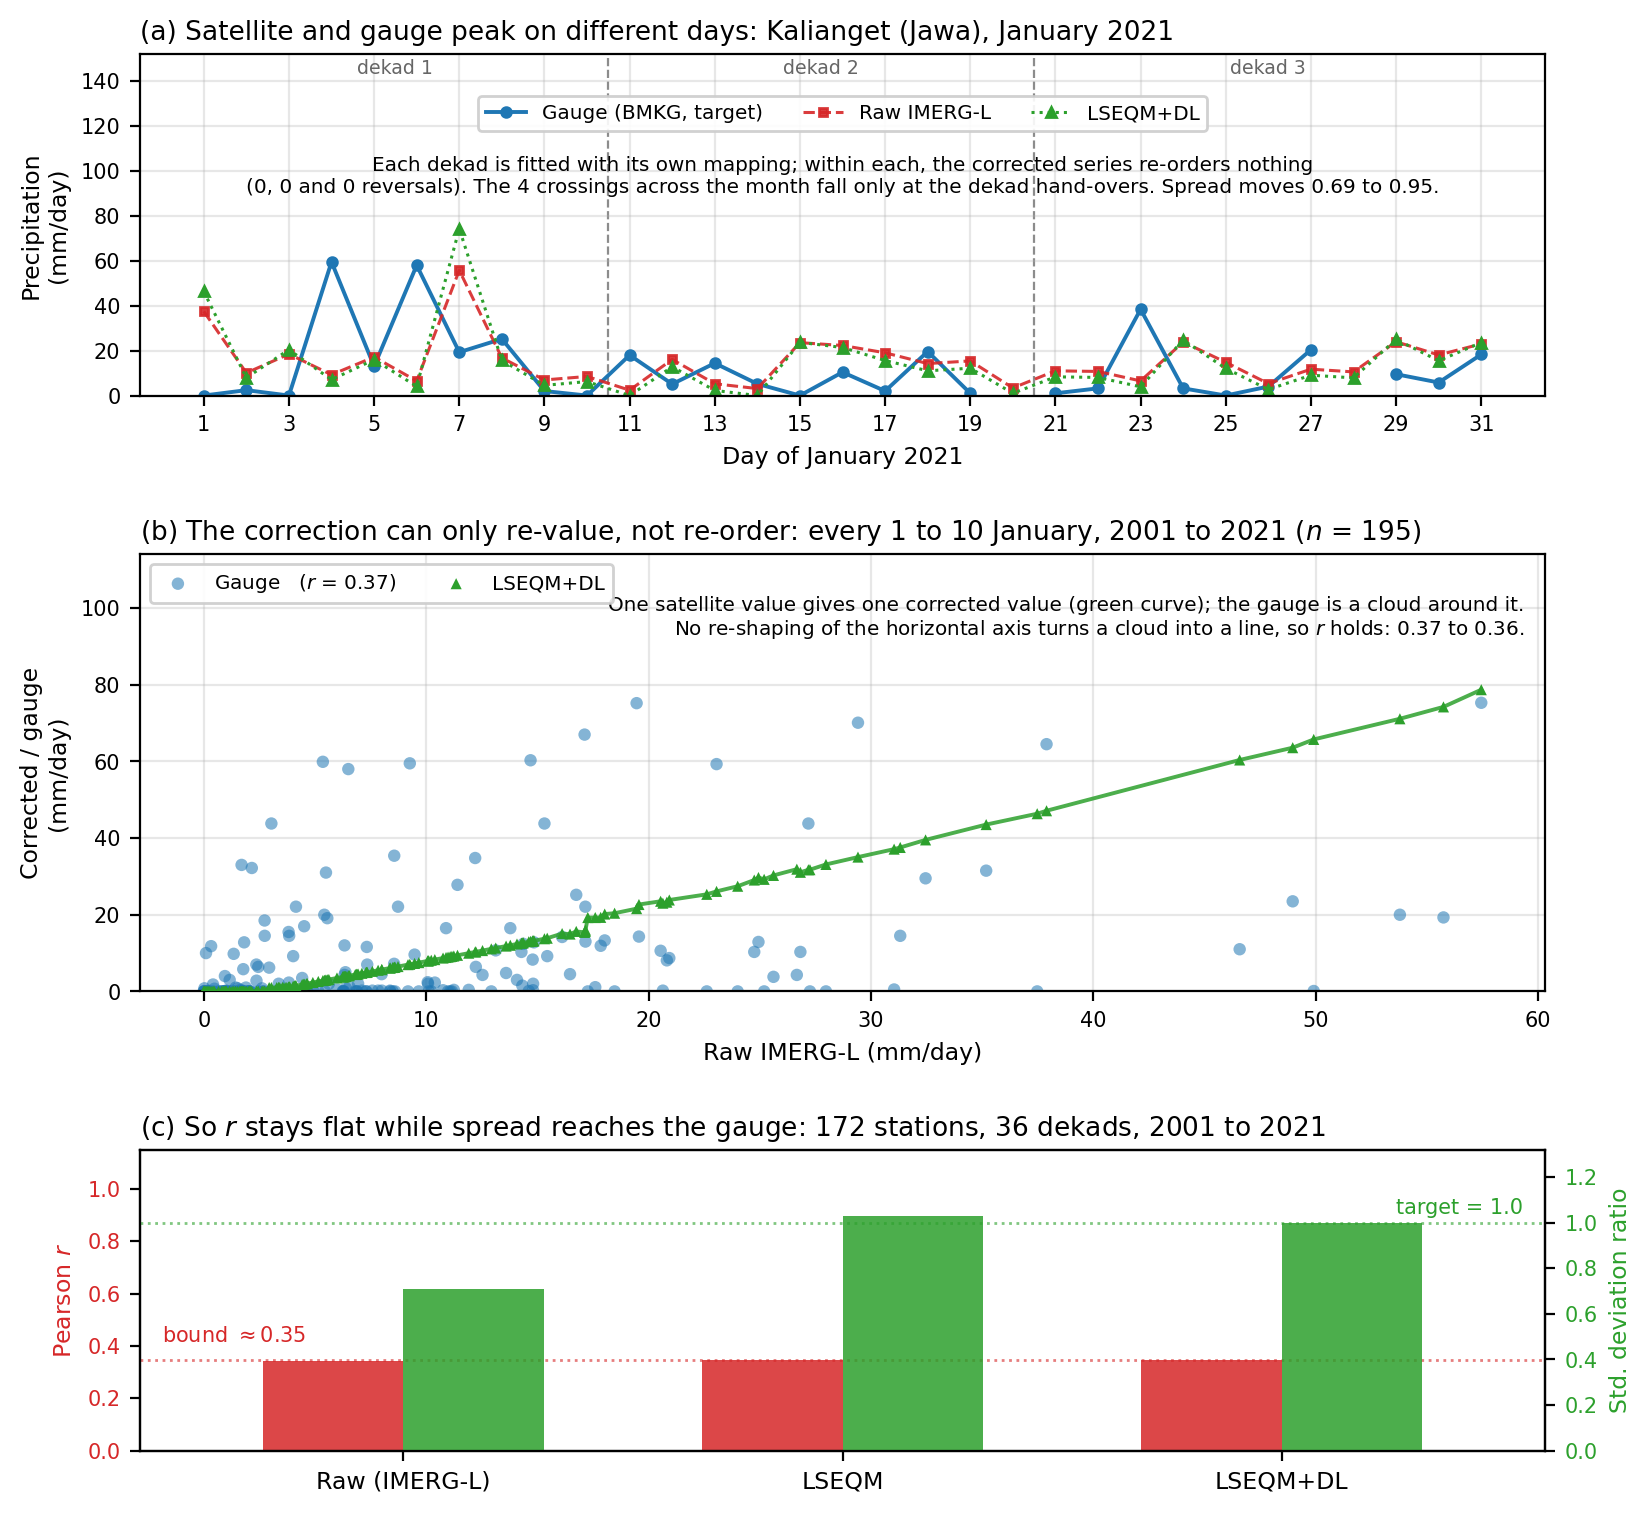
\includegraphics[width=\figFiveOneWidth\textwidth]{fig_thesis_05_bound_schematic.png}
\caption[The theoretical bound on Pearson $r$ under marginal correction]{The theoretical bound on Pearson $r$ under marginal
correction, on real data at one station and over the validation
network\label{fig:bound-schematic}}
\end{figure}

The first component is rank preservation. Monotone,
rank-preserving quantile mapping, the family to which empirical quantile mapping
with Gamma kernels and GPD tail adjustment both belong, preserves the rank order of values at each
location \citep{ref:cannon2015}. If the satellite reports a higher
value on day $i$ than on day $j$ before correction, and both days
fall in the same dekad, it will report a value no lower on day $i$
than on day $j$ after correction; across a dekad boundary a
different mapping applies, which produces the dekad-boundary
crossings visible in Figure~\ref{fig:bound-schematic}a. The
day-by-day pairing of satellite values to gauge values is fixed by
the satellite product itself; no operation in a marginal correction
pipeline can move a value from one day to its neighbour. The mapping
is monotone but not strictly so, because dry-day frequency matching
sends a substantial fraction of low-rain days to exactly zero: this
creates ties, but no reversals, so the day-ordering is preserved
without the map being one-to-one.

The CNN
refinement stage relaxes the rank-preservation property at
each pixel because the $3 \times 3$ convolution mixes information
from neighbouring pixels at the same timestep, but it does not
reorder the time series at a single pixel beyond the small
residual it learns to add on top of LSEQM. The size of that
relaxation is measurable. At the station of
Figure~\ref{fig:bound-schematic}, over the $195$ paired days of the
first January dekad shown in panel~(b) and with the raw series
sorted ascending, LSEQM reorders none of the $194$ adjacent pairs,
whereas LSEQM+DL
reorders six and introduces roughly $1$~mm of spread at equal raw
value across the $21.5\%$ of days the refinement touches. The
relaxation is therefore real but marginal, and it buys no temporal
skill: $r$ against the gauge moves from $0.368$ to $0.357$ on that
sample.

Because the residual
training target is the LSEQM-to-Climate Prediction Center (CPC) Unified Gauge-Based Analysis of Global Daily Precipitation (CPC-UNI) difference rather than
a free reconstruction, the temporal ordering at each pixel after
the CNN refinement remains a small perturbation of the LSEQM
ordering. The rank-preservation argument therefore carries through
to the full pipeline at the level of pixel-wise paired time series,
which is the level at which Pearson $r$ against an external gauge
is computed.

The second component is variance inflation without skill gain.
A pointed critique of quantile mapping in regional climate
applications \citep{ref:maraun2013} established that quantile
mapping widens spread to match the marginal target without
improving time-dependent skill, because spread alignment and
day-by-day pairing are independent properties of a paired
series. Within a single dekad at a pixel, Linear Scaling is a
positive rescaling, which leaves the Pearson correlation exactly
where it was; the nonlinear EQM and GPD stages introduce no rank
reversals, so they cannot re-pair a satellite day with a different
gauge day. The exact invariance under Linear Scaling holds only at
that granularity.

A correlation pooled across dekads and pixels
mixes samples that each carry a different scaling factor, so the
pooled value shifts slightly even under Linear Scaling: against the
BMKG stations it moves by $+0.003$
(Section~\ref{sec:results-intercomparison}).
Neither step fixes the Pearson correlation exactly, because the map
is nonlinear and dry-day matching creates ties, but in practice the
correlation is observed to move only within single-pixel sampling
uncertainty. Even a perfect spread match therefore has little
purchase on $r$. The combination of rank
preservation and spread-without-skill yields the headline
proposition of this chapter:

% Keep the indented proposition together on one page: ~8 lines of
% quote text + small breathing room. If less than that remains on the
% current page, force a break so the whole block lives on the next.
\needspace{10\baselineskip}
\begin{quote}
\emph{A monotone, rank-preserving marginal correction cannot
re-order a satellite series in time, so it cannot manufacture
day-by-day agreement with an external paired gauge that the raw
series does not already have. The Pearson correlation is therefore
held near its raw value; the residual movement comes only from the
nonlinear reshaping of amplitudes and the small rank-changing
contribution of the spatial CNN refinement, and is observed to
stay within single-pixel sampling uncertainty.}
\end{quote}

\noindent The proposition is what the four-pillar pattern and the
flat $r$ pattern are jointly expressing.

The bound is not a claim that $r \approx 0.35$ is the value a daily
product must take. Reported daily correlations vary widely with the
setting: against the dense Chinese gauge analysis the median for
IMERG is near $0.75$, while over the Indonesian Maritime Continent
the daily value is lower and rises substantially only at dekadal or
monthly aggregation (Section~\ref{sec:lit-bounds}). The corrected
LSEQM+DL value of $0.348$, measured per pixel against the
in-sample CPC-UNI target at the native UTC window and averaged over
the $36$ dekadal windows, sits at the low end of that spread. What
the bound asserts is narrower and is what the stage comparison
tests: whatever the starting value, marginal correction does not
raise it.

The ceiling has two
contributors. The first is a calendar-window component: the
UTC-dated IMERG-L archive coincides with the CPC-UNI calibration
label but is offset by about one day from the local-day BMKG
morning-observation label. Against BMKG the daily correlation
is therefore suppressed under UTC alignment and recovered by re-aggregating
the satellite to the local-observation window: a fixable metadata
artefact rather than a satellite limit, quantified in
Section~\ref{sec:discussion-subdaily}. The second is the residual
timing accuracy of the underlying retrieval, which lies upstream
of every step in the pipeline and requires methods outside the
marginal correction family
(Section~\ref{sec:discussion-paths}).
Section~\ref{sec:discussion-ops} returns to the operational
significance of this split.

The pattern is
also stable across the calendar year.
Figure~\ref{fig:taylor-monthly} aggregates the BMKG Taylor
analysis by month and shows that the angular position of the
three method symbols, which encodes correlation, sits at the
same place in every month. The radial position, which
encodes the standard deviation ratio, sits near unity for LSEQM
and LSEQM+DL and short for LS. The bound is therefore not a
seasonal artefact and does not depend on the wet- or dry-season
sample composition.

\begin{figure}[H]
\centering
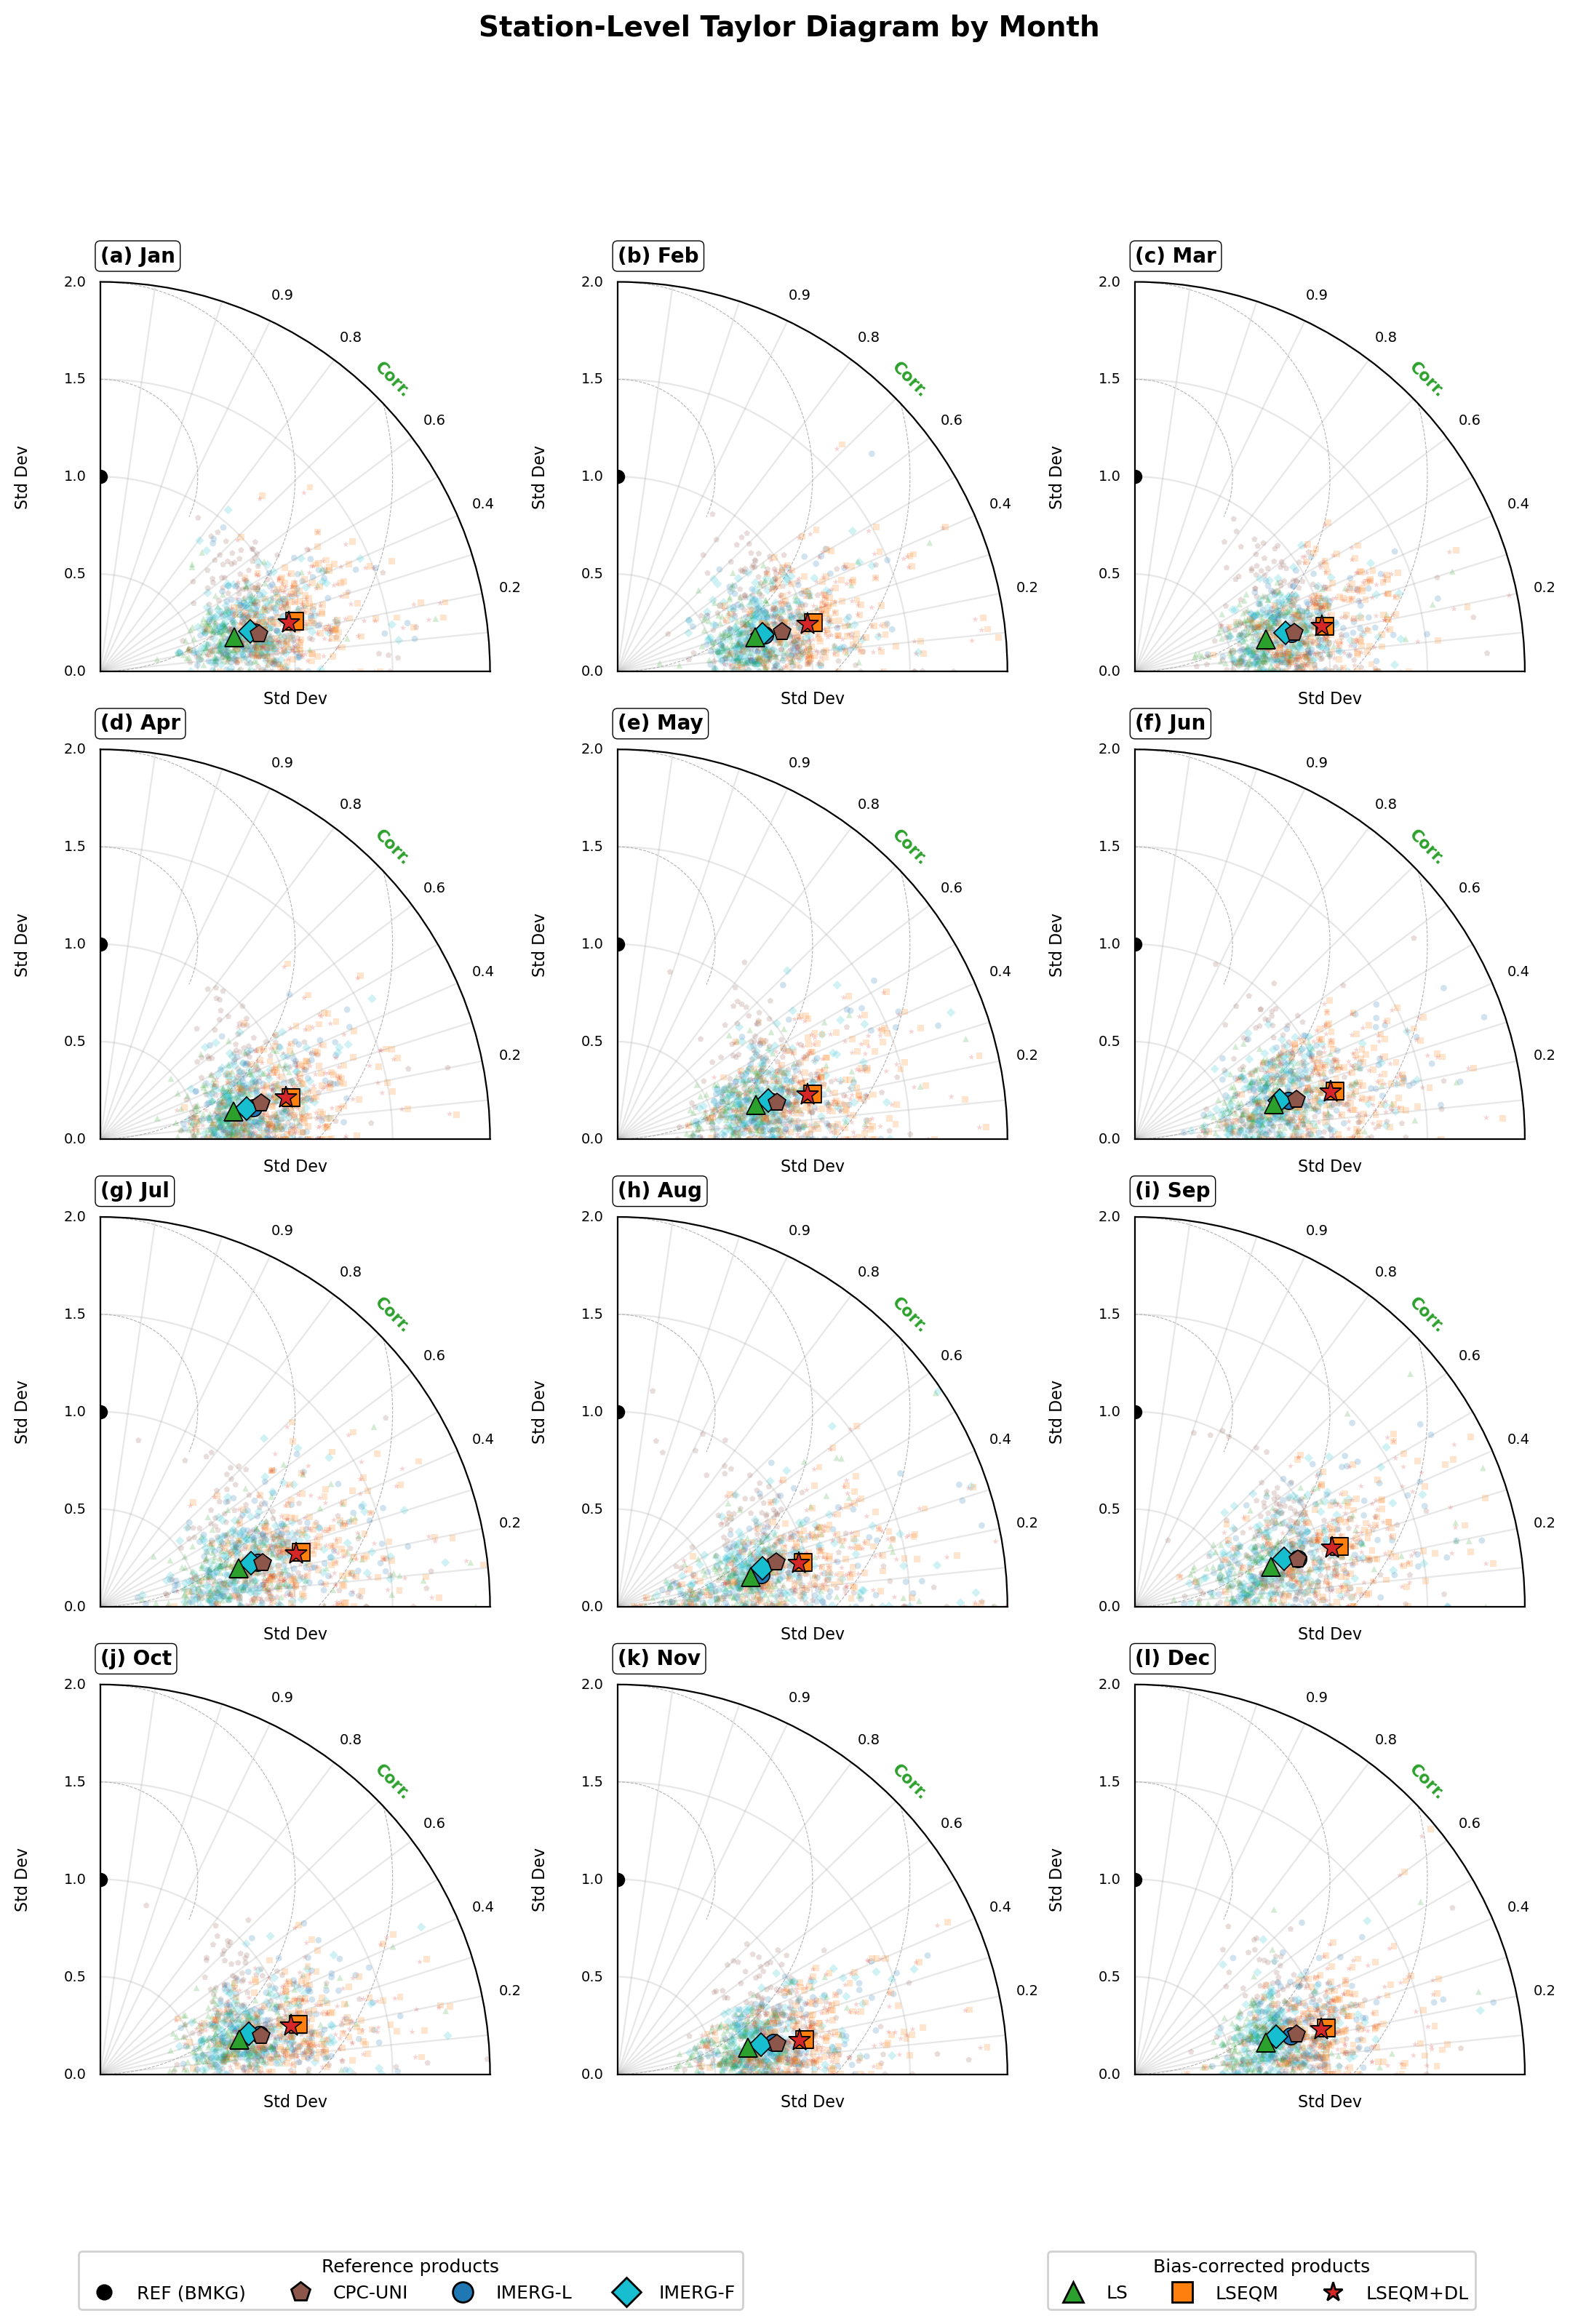
\includegraphics[width=\figFiveTwoWidth\textwidth]{fig_thesis_05_taylor_monthly.png}
\caption[Monthly Taylor diagram aggregated across the BMKG validation stations]{Monthly Taylor diagram aggregated across the $171$ BMKG
stations carrying a valid per-dekad correlation\label{fig:taylor-monthly}}
\end{figure}

A complementary reading uses the canonical decomposition of the
mean squared error into a bias term, a spread-mismatch term, and a
correlation-residual term \citep{ref:gupta2009}. The bias term is
moved cleanly by the Linear Scaling stage, and the spread-mismatch
term is driven toward zero by the EQM stage as the
standard-deviation ratio moves to unity and beyond. The
correlation-residual
term, equal to
$2\,\sigma_{\text{sat}}\,\sigma_{\text{gauge}}\,(1-r)$, is
the mechanism through which the RMSE actually increases between
LS ($13.1$ mm per day) and LSEQM+DL ($14.1$ mm per day). Once the
satellite spread is inflated to match the reference spread without
any improvement in $r$, this term grows, because
$\sigma_{\text{sat}}$ has risen toward $\sigma_{\text{ref}}$ while
$(1-r)$ stays near $0.65$, and its growth outweighs the vanishing
spread-mismatch term $(\sigma_{\text{sat}} - \sigma_{\text{ref}})^2$.
The whole decomposition is measured in sample against CPC-UNI,
where the standard-deviation ratio does not stop at unity but
overshoots to $1.15$; the convergence to $1.00$ reported in
Chapter~\ref{chap:results} is the out-of-sample result against the
BMKG stations, and mixing the two would misstate the mechanism.

This is the
variance-inflation-without-skill effect identified for quantile
mapping in regional climate applications \citep{ref:maraun2013}:
matching the spread without matching the timing increases the
squared error at the corrected stage relative to the
under-spread raw stage. NSE follows the same logic by
construction. The fact that three temporal-skill diagnostics
fail to improve and one improves only mildly does not indicate
failure; it indicates that the pipeline is doing exactly what
marginal correction can do, and not what it cannot.

The framing of this pattern matters for the wider field. In the
absence of stage-resolved attribution, a study that reported only
the aggregate $r$ would conclude that the LSEQM+DL framework
delivers little improvement over raw IMERG-L, and the substantial
movement in the value, distribution, extreme, and detection
pillars would be invisible. The four-pillar verification framework
of Section~\ref{sec:methods-metrics}, paired with Pearson $r$ as a
separate temporal-skill diagnostic rather than as an
all-encompassing skill score, lets the structural limit and the
methodological improvement appear in the same report. This is the
verification posture the present work argues for, and it is a
posture that the parallel reproducibility contribution
(Section~\ref{sec:discussion-reproducibility}) lets any reader
independently reconstruct on their own data.


% ============================================================
\section{Interpreting the Optimal Aggregation Window}\label{sec:discussion-subdaily}
% ============================================================

\textbf{The calendar-window mismatch.} The bound in
Section~\ref{sec:discussion-bound} predicts that
marginal correction cannot lift Pearson~$r$ above the timing
quality of the underlying retrieval, but it does not decompose
the absolute ceiling into its components. One component the bound
discussion does not isolate is the calendar-window definition used
to label each daily value. IMERG-L distributes daily totals
aggregated over the Coordinated Universal Time (UTC) calendar day~\citep{ref:imergdl07}.
The BMKG climatological-station daily totals are reported
under the morning-observation convention specified by Head of BMKG
Decree SK.32/TL.202/KB/BMG-2006 \citep{ref:bmkg2006sk32},
consistent with the World Meteorological Organization principle of
measuring daily precipitation at fixed observation times common to
the network \citep{ref:wmo2018no8}. Under that convention the
rainfall total assigned to
date~$d$ is the 24-hour accumulation ending at the BMKG morning
observation on date~$d$, nominally $07{:}00$ local time. Because
Indonesia spans the three local-time zones WIB, WITA, and WIT
(UTC$+7$, $+8$, $+9$), the BMKG daily window ends near $00{:}00$
UTC for WIB stations and a few hours earlier for stations east of
the WITA boundary. The daily IMERG-L window and the daily BMKG
window are therefore offset by approximately 24~hours in the
worst case, and the daily product values labelled by the same
calendar date refer to different 24-hour rainfall periods.

Section~\ref{sec:results-window} established empirically that
re-aggregating the half-hourly source recovers the GPM-era
correlation from $r = 0.20$ at the UTC-day window to $r = 0.57$ at
$h = -23$~h. That offset is not a fitted parameter but the
signature of the gauge convention. Under the morning-observation
rule, the total assigned to date~$d$ is the 24-hour accumulation
ending at the $07{:}00$ observation; for a WIB station this window
is $[00{:}00\,\text{UTC}\ (d{-}1),\ 00{:}00\,\text{UTC}\ (d)]$,
which begins $24$~h before the UTC day the archive labels with
date~$d$. The empirical peak at $-23$~h sits within the two-to-four
hour spread expected from varying station observation times,
retrieval blending across the half-hourly timestamp, and the
diurnal phase of maritime-continent convection.

\textbf{Convention dependence of the gauge references.} The two
gauge references differ in both the hour at which a daily total
closes and the date it is then given, and resolving the difference
sharpens the picture. The
gridded CPC-UNI archive dates each daily total by a per-cell
end-of-day field; for every Indonesian cell this field is
$24$~hours, so the total closes at $00{:}00$ UTC and is assigned
the UTC calendar date \citep{ref:cpcuni_readme}, whereas the BMKG
archive keeps the local morning-read date one calendar day later.
The CPC-UNI total therefore coincides with the UTC-day IMERG-L
window, while the BMKG label sits one calendar day from it. A day-shift
test confirms the split directly: the IMERG-versus-CPC-UNI daily
correlation is highest at the native same-date pairing and falls
when CPC-UNI is shifted by a day, whereas the IMERG-versus-BMKG
correlation is highest only after the satellite is re-aggregated
to the local-observation window (Figure~\ref{fig:convention}a).
The calendar-window offset is thus specific to the BMKG
labelling: IMERG and CPC-UNI share the UTC day and carry no
window offset, so the calibration target is already consistent
with the satellite.

At
the station locations both references reach the same
retrieval-limited correlation (approximately $0.57$ in the GPM
era), but at offset windows: CPC-UNI at the UTC day and BMKG at
$h = -23$~h. The practical consequence is that daily
satellite-gauge correlation is convention-dependent: no single
calendar label maximises agreement with both references at once,
so a corrected product is best distributed on an explicit
local-observation day with all references harmonised to it
(Figure~\ref{fig:convention}b). The
agreement attainable after harmonisation remains bounded by the
retrieval timing accuracy, so the residual ceiling cannot be
raised by relabelling and requires sub-daily or multivariate
methods (Section~\ref{sec:discussion-paths}).

\begin{figure}[H]
\centering
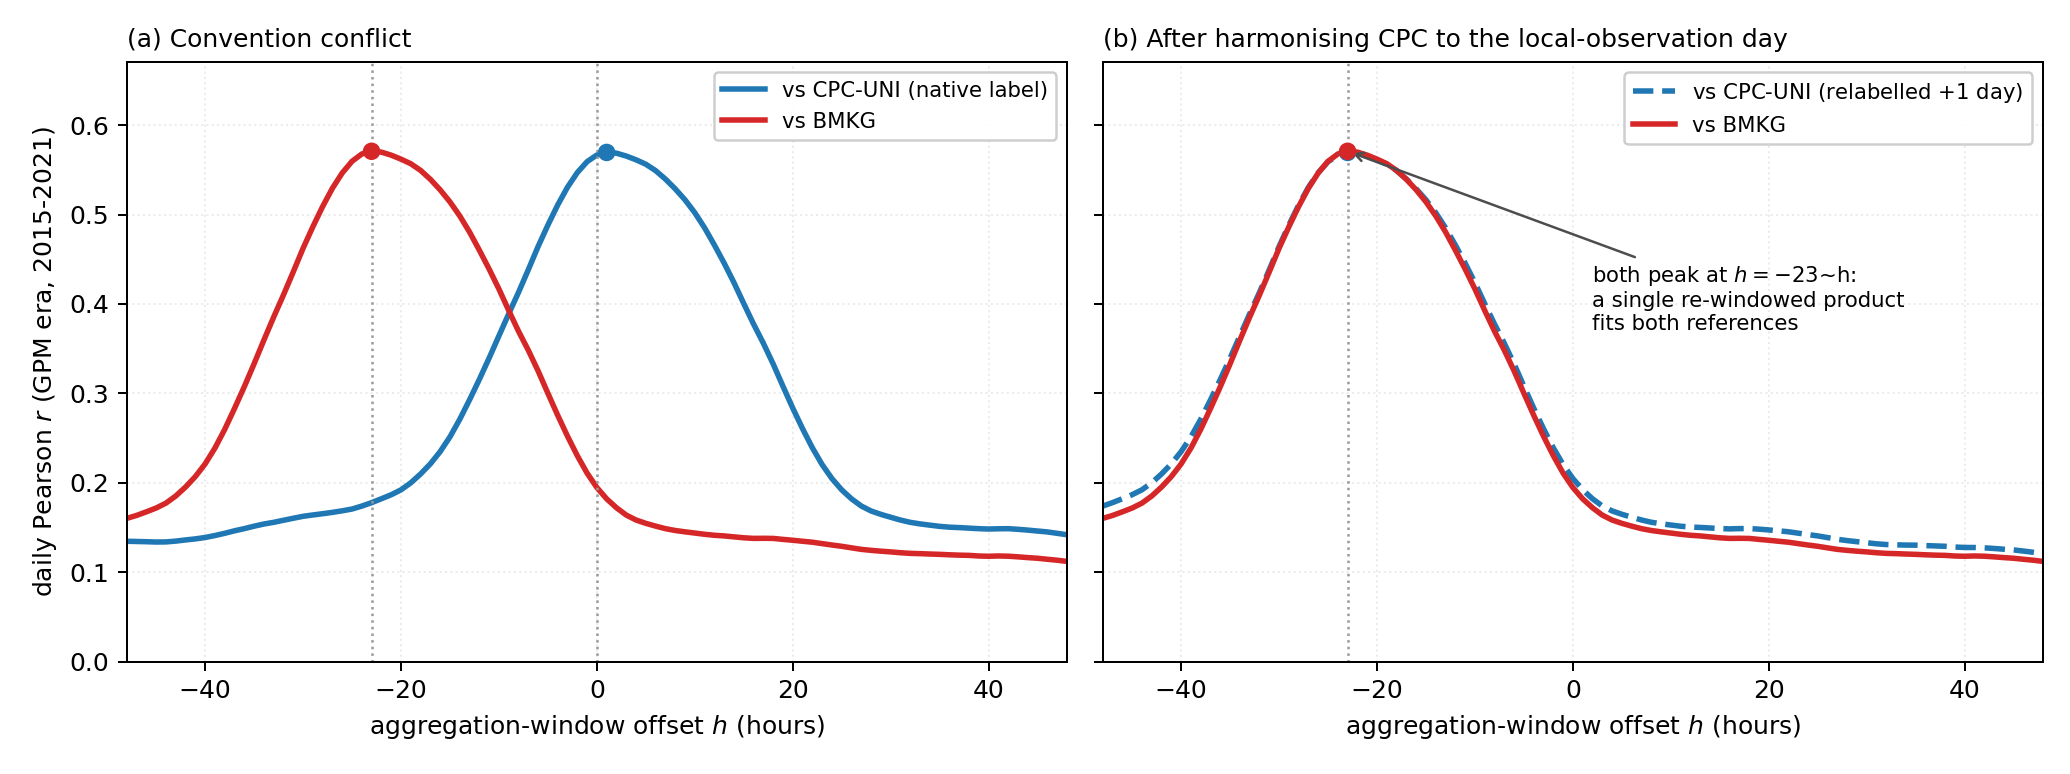
\includegraphics[width=\figFiveConventionWidth\textwidth]{fig_thesis_05_convention.png}
\caption[The calendar-window convention conflict and its resolution]{Daily
IMERG correlation against CPC-UNI and BMKG versus aggregation-window offset at the
$178$ station locations with valid half-hourly coverage (GPM era): (a) the convention
conflict and (b) its resolution by relabelling CPC-UNI to the local-observation day.\label{fig:convention}}
\end{figure}

The diagnostic pools the $178$ stations with valid half-hourly
coverage, a slightly larger set than the $172$ out-of-sample
validation stations used for the headline results.
Table~\ref{tab:convention} lists the four correlations directly: each
reference reaches approximately $0.57$ at its own optimal window
(CPC-UNI at the UTC day, BMKG at $h = -23$~h) and falls to $0.18$
to $0.20$ at the other, a mirror-image structure across the two
calendar labels.

\begin{table}[H]
\centering
\caption[Convention-dependence of the daily satellite-gauge correlation]{Daily
IMERG Pearson $r$ at the $178$ BMKG station locations (GPM era), under the UTC
and the local-day ($h=-23$~h) aggregation windows\label{tab:convention}}
\begin{tabular}{lcc}
\toprule
Reference & UTC window ($h=0$) & Local-day window ($h=-23$~h) \\
\midrule
CPC-UNI (calibration) & $\approx 0.57$ & $\approx 0.18$ \\
BMKG (validation)     & $\approx 0.20$ & $\approx 0.57$ \\
\bottomrule
\end{tabular}
\end{table}

\textbf{Whole-domain confirmation against CPC-UNI.} The
station-based day-shift test extends to a continuous map by
repeating the offset sweep against the gridded CPC-UNI analysis at
every $0.5^\circ$ cell (Figure~\ref{fig:gridded-cpc}). At
CPC-UNI's native UTC labels the optimal offset is $h^\star
\approx 0$ across the gauge-constrained western and central cells
(Figure~\ref{fig:gridded-cpc}a), the whole-domain signature of
CPC-UNI sharing the IMERG-L UTC day; relabelling CPC-UNI to the
local-observation day moves the optimum to $h^\star \approx -23$~h
everywhere (Figure~\ref{fig:gridded-cpc}b). The offset is
identical in the timing-imprecise TRMM-input era ($2001$ to
$2013$) and the GPM era, which is consistent with a labelling
effect rather than a property of retrieval skill. Pooled over the
$134$ cells that hold
BMKG stations the correlation reaches $0.56$ in the GPM era
(Figure~\ref{fig:gridded-cpc}c, bold), close to the
per-station diagnostic and Table~\ref{tab:convention}; pooled over
the whole domain it falls to $0.334$ (faint), close to the
in-sample whole-coverage correlation against CPC-UNI
(Table~\ref{tab:cpc-corr-dist}), diluted by the data-sparse east
where the contributing-gauge network thins and $h^\star$ turns noisy. The era gain against CPC-UNI is modest
($0.51$ to $0.56$) next to the point-gauge recovery ($0.36$ to
$0.57$) because the smoothed $0.5^\circ$ analysis forgives the
point-representativeness noise that depresses the early-era
point-gauge correlation, so both references converge near $0.56$
to $0.57$ once the retrieval resolves the diurnal cycle.

\begin{figure}[H]
\centering
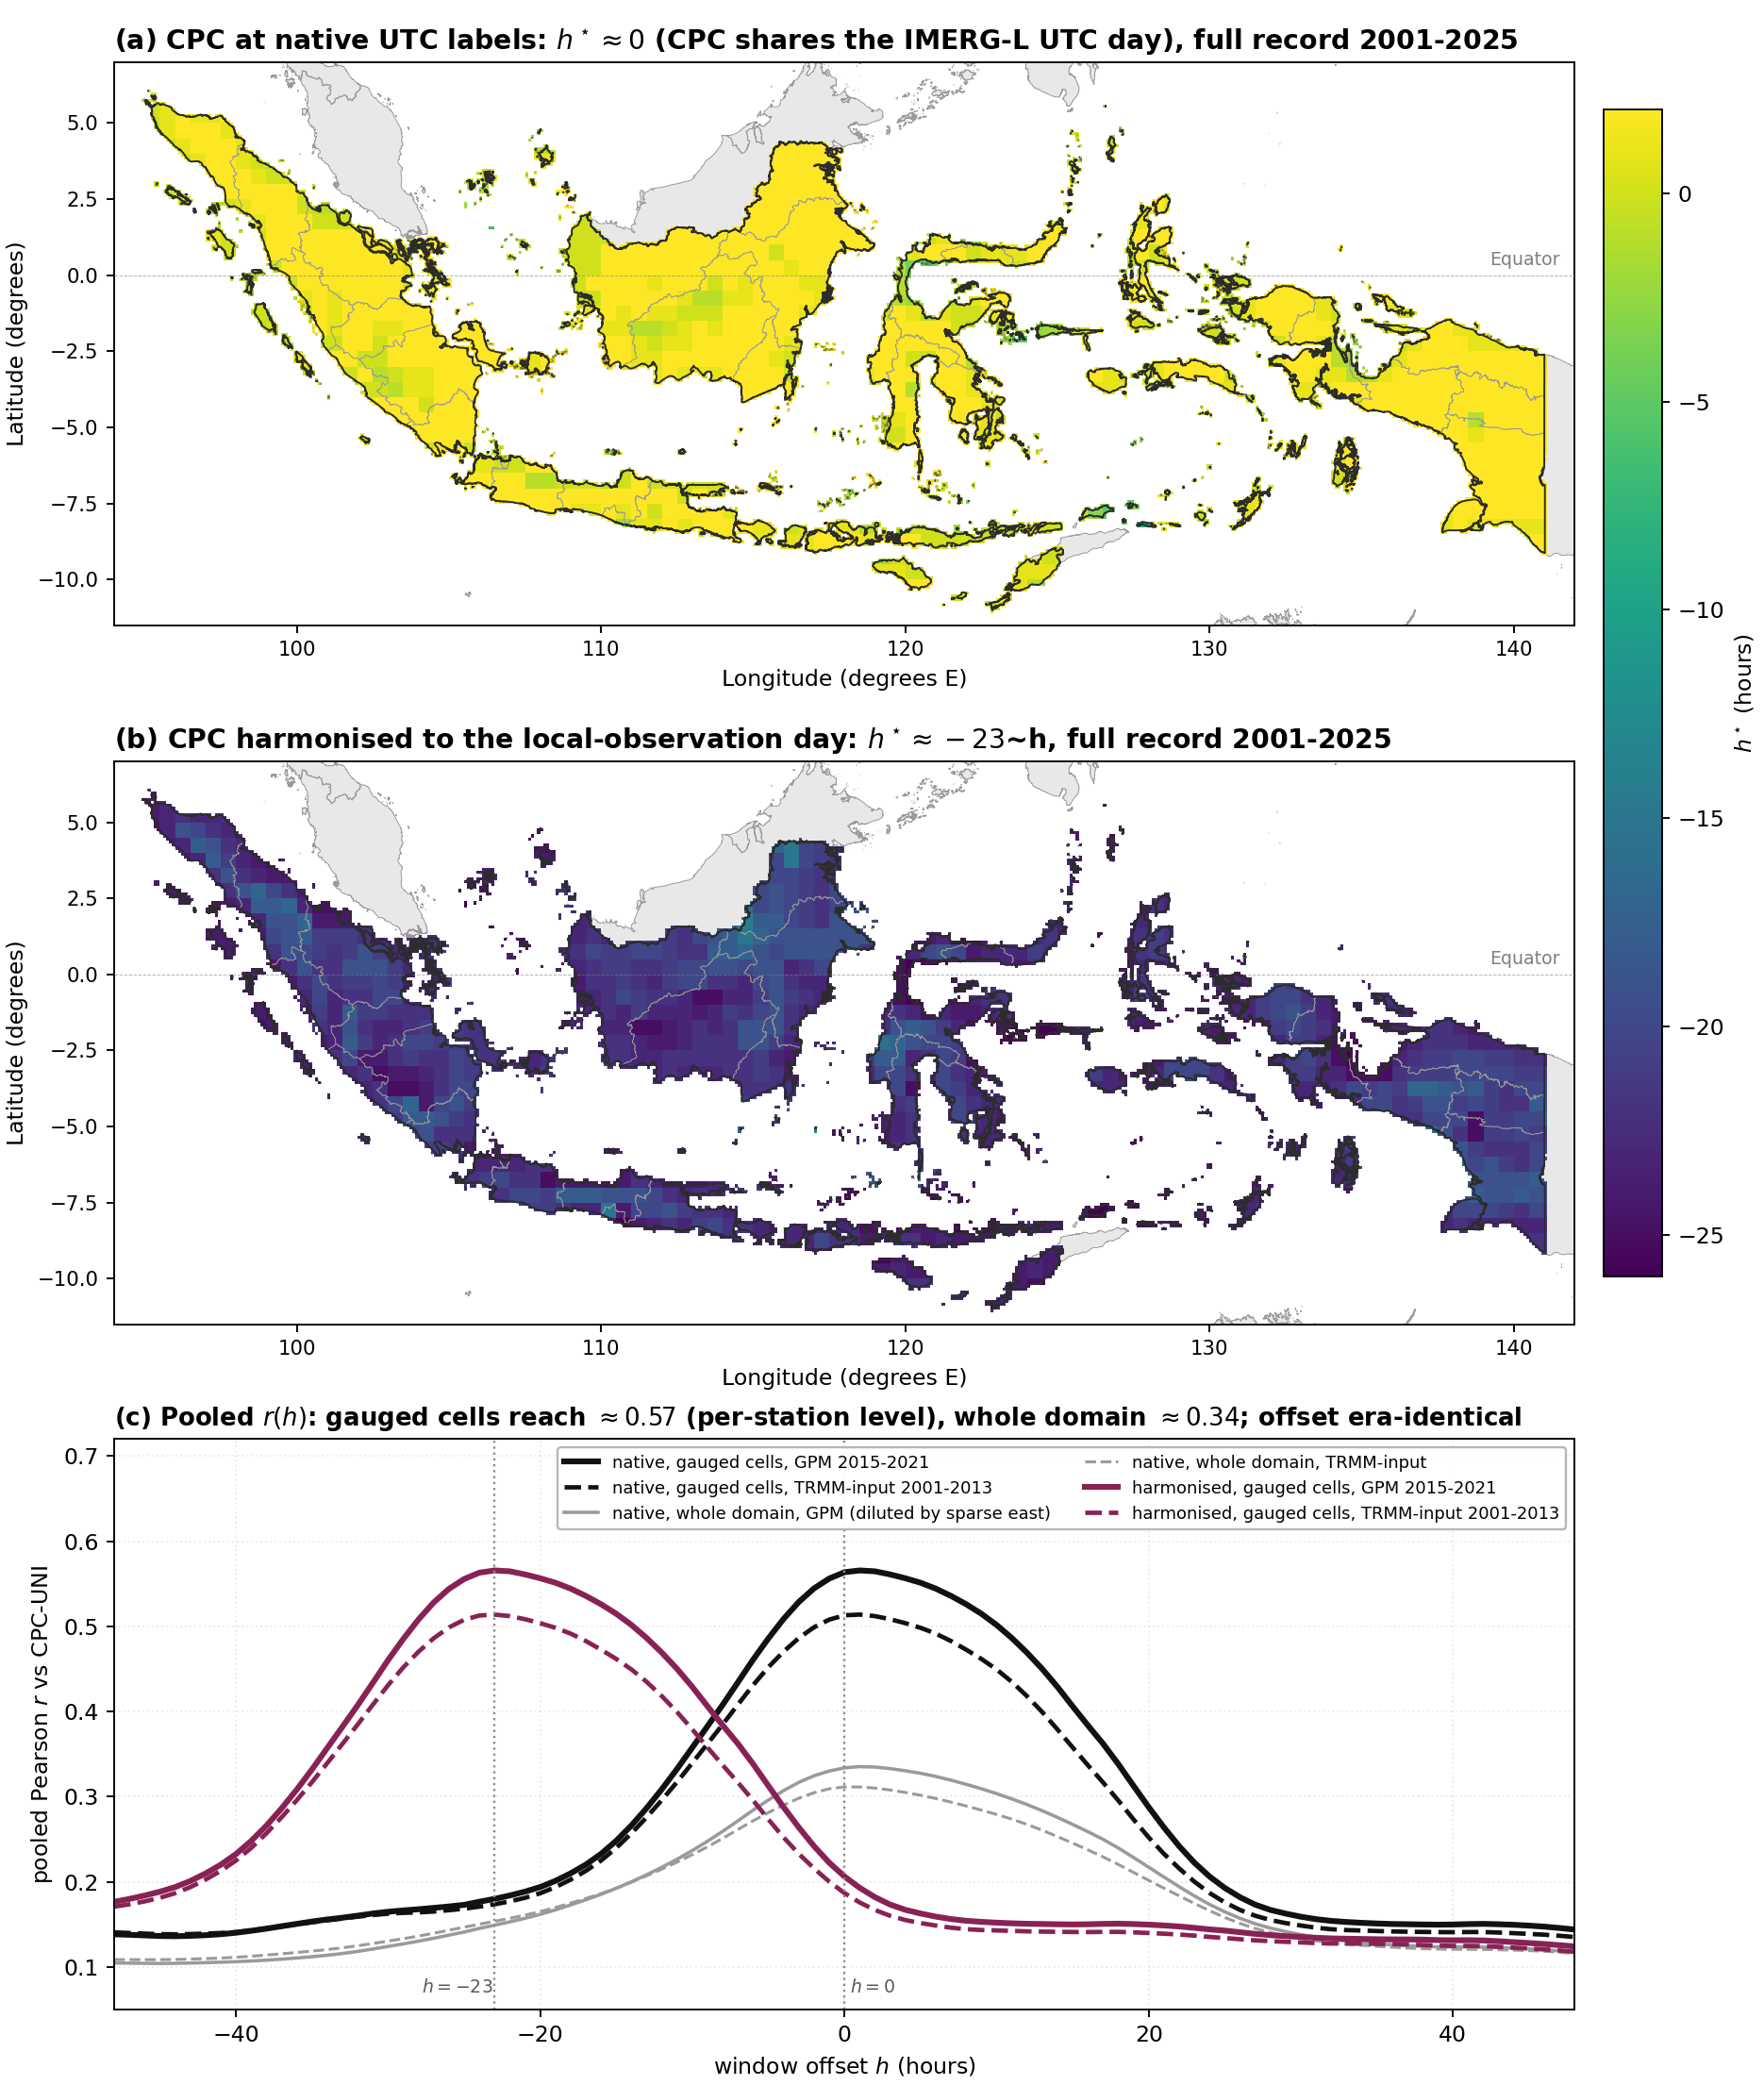
\includegraphics[width=\figFiveGriddedCpcWidth\textwidth]{fig_thesis_05_gridded_cpc.png}
\caption[Gridded window offset against CPC-UNI over the full record]{Gridded
window-offset diagnostic against CPC-UNI over the full record\label{fig:gridded-cpc}}
\end{figure}

\textbf{Timezone bands and the single peak.} The single broad
peak shared across the WIB, WITA, and WIT bands,
rather than three distinct peaks at $-7$, $-8$, and $-9$~h, shows
that the morning-observation convention dominates over the
local-midnight timezone offset. The reason is that the observation
time is a legal-clock time, a step function of the timezone region,
not a solar time that varies continuously with longitude. Every
station within a band therefore shares the same UTC window
boundary, which cancels the continuous solar drift and leaves no
systematic longitudinal gradient in $h^{\star}$
(Section~\ref{sec:results-window}); the residual two-hour spread
reflects the diurnal-phase variation and the breadth of the
correlation peak. One consequence is a small artefact at timezone
boundaries: two stations a few kilometres apart but on opposite
sides of the WIB/WITA line use legal reference times one hour
apart, so their gauge windows differ by one hour in UTC despite
near-identical rainfall and near-identical solar time. This is an
intrinsic limitation of attributing a legal-clock observation to a
spatially continuous field, and it argues for defining any
operational window from the gauge reporting convention rather than
from solar geometry.

\textbf{Confinement to the GPM era.} The recovery is confined to
the GPM era, and the reason is
instructive (Figure~\ref{fig:window-precision}). Before the full
GPM constellation, the half-hourly field places a given day's rain
with roughly one-day uncertainty: its correlation with the gauge on
the day before a wet day is nearly as high as on the wet day
itself, so no realignment of the 24-hour window can recover the
day-by-day match, and the correlation stays near $r = 0.36$ at
every offset. The GPM-era field is day-precise, so aligning the
window to the gauge convention recovers the correlation. The
window-offset search therefore doubles as a diagnostic of a
product's day-to-day temporal precision, and it places the IMERG
precision improvement at the $2014$ to $2015$ transition to the
GPM constellation. A telling detail is that in the early era the
correlation optimum sits near the UTC day rather than at the
convention offset, consistent with a field too temporally smeared
to register the gauge window; the reason the optimum takes this
sign in the early era is not established here. The era dependence is
independently corroborated over Indonesia: an evaluation in
mountainous Sumatra attributes the improved daily IMERG accuracy in
the GPM era to the denser passive-microwave constellation and the
algorithm advances introduced with the 2014 GPM Core launch
\citep{ref:ramadhan2024sumatra}.

\begin{figure}[H]
\centering
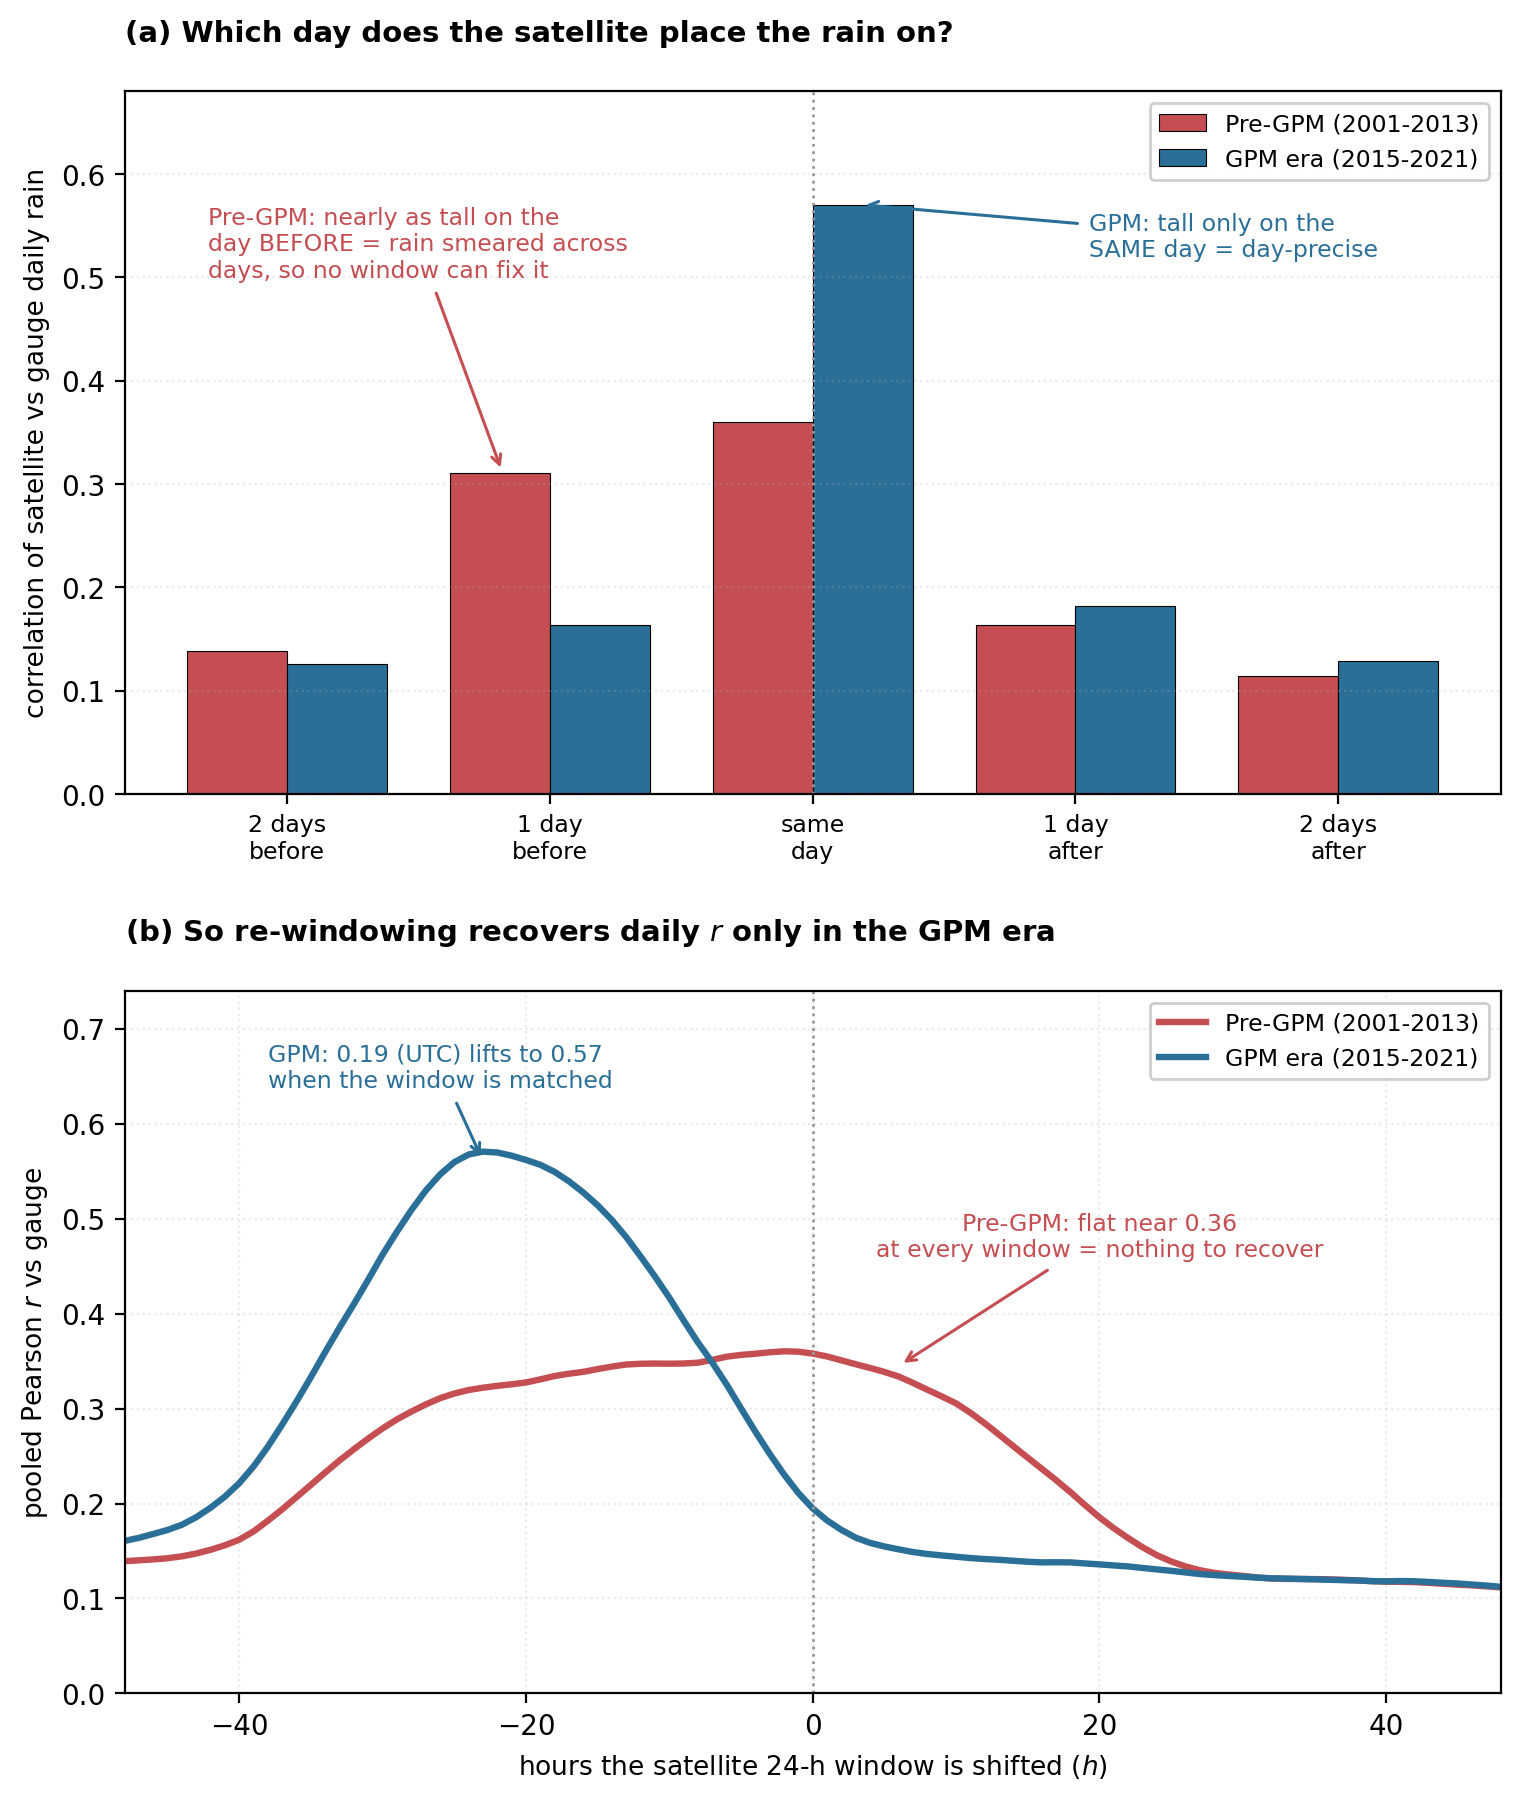
\includegraphics[width=\figFiveWindowPrecisionWidth\textwidth]{fig_thesis_05_window_precision.png}
\caption[Why the window recovery is confined to the GPM era]{Day-offset
correlation (a) and window-offset correlation (b) for the pre-GPM and
GPM eras, showing why the window recovery is confined to the GPM
era.\label{fig:window-precision}}
\end{figure}

\textbf{Calibration and validation.} The two gauge references are
assembled under different conventions. CPC-UNI closes each daily
total at $00{:}00$~UTC and assigns it the UTC date
\citep{ref:cpcuni_readme}, while BMKG closes at the morning
observation and assigns the local date under
SK.32/TL.202/KB/BMG-2006 \citep{ref:bmkg2006sk32}. The two archives
therefore label a day about one day apart, and the
window mismatch surfaces at only one end of the
pipeline. The CPC-UNI label coincides with the UTC-day IMERG-L
archive, so the calibration pairing carries no window offset; the
BMKG label sits one day from the archive, so the $-23$~h offset
appears only in the validation pairing. The diagnostic was
performed against BMKG because it provides the independent
out-of-sample station network at point-pixel resolution. The
four-pillar metrics (value, distribution, extreme, detection) are
functions of the marginal distribution and of categorical events
and are therefore window-invariant when the daily sample
composition is preserved, so the calibration of LS, EQM, and GPD
against CPC-UNI remains correct under the present window choice.
Pearson~$r$ is the only metric the window choice affects, and the
effect is confined to the comparison against the local-day BMKG
gauges.

\textbf{The monthly scale and the headline ceiling.} Because the
four-pillar metrics are essentially window-invariant (the daily
sample composition being nearly preserved across offsets), only the
absolute Pearson~$r$ depends on the aggregation window, and
aggregating to the monthly scale dissolves even that dependence:
Section~\ref{sec:results-window} reports a monthly correlation near
$0.80$ whether the daily windows are UTC-aligned or gauge-matched.
The product therefore carries the monthly rainfall faithfully while
mis-assigning it across day boundaries at the daily scale, which
locates the daily ceiling in the timing of the day-by-day pairing
rather than in the amount of rainfall captured. The bound of
Section~\ref{sec:discussion-bound} separates accordingly into a
calendar-window component, the larger and recoverable part, and a
residual retrieval-skill component that no window choice removes.
The correlation against CPC-UNI, the in-sample calibration target,
holds near $0.35$ (Table~\ref{tab:cpc-corr-dist}) and is left
pinned close to its raw value by the marginal-correction pipeline, which
introduces no rank reversals in its LSEQM stages and only a small
rank-changing CNN contribution, so Pearson $r$ against CPC-UNI
changes only within sampling noise. The independent correlation
against the BMKG point gauges is lower and era-dependent; over the
GPM era it rises from $0.20$ at the UTC-day window to $0.57$ at the
gauge-matched window (Section~\ref{sec:results-window}), the
recoverable calendar-window component in action.

\textbf{Scope and bounds of the contribution.} The window-offset
search adopted here is the gauge-timing inference
of \citet{ref:beck2019}, developed for global precipitation
merging. Evaluations over the Maritime Continent pair the two
series in Coordinated Universal Time rather than on the gauge
reporting day \citep{ref:ramadhan2022ts}, and daily
bias-correction workflows likewise report correlation
against a fixed window \citep{ref:ramadhan2024sumatra, ref:suhartanto2025}. The contribution here is therefore not
the offset search but its regional grounding in the BMKG
convention, its propagation into the verification of a correction
pipeline, and the quantified recovery with its seasonal, spatial,
and era structure. A broader implication, which this single-region
result does not establish, is that daily satellite-gauge
correlations reported against a fixed UTC window may understate a
product's true day-by-day skill \citep{ref:tang2020,
ref:ramadhan2022ts}; this is offered as a hypothesis for
multi-region testing, not a conclusion.

The recovery is bounded, and the bounds govern how it should be
read. It is confined to the GPM era; it is partial, lifting the
pooled correlation to approximately $0.57$ rather than to unity; it
is an upstream re-aggregation of the raw half-hourly archive,
outside the LSEQM+DL pipeline, which by construction cannot move
$r$. It requires access to the half-hourly source, since an
already-aggregated daily archive cannot be re-windowed; the
$-23$~h offset is specific to the local-day morning convention and
must be re-derived for any other reporting practice; and it acts on
the daily correlation alone, leaving the four pillars and the
monthly skill unchanged. The operational re-aggregation of the
daily archive over a gauge-matched window is a single-stage change
to the pre-processing, identified as the most actionable path
forward in Section~\ref{sec:discussion-paths}.


% ============================================================
\section{Operational Implications}\label{sec:discussion-ops}
% ============================================================

The split between four-pillar improvement and flat temporal skill
translates directly into operational guidance for users of the
corrected IMERG-L product. The pipeline corrects what marginal
correction can correct; users should match their application to
the metrics that moved, not to the ones that did not. The
guidance organises around the question of whether the application
depends on the daily distribution or on the day-by-day pairing of
satellite values to a specific calendar day.
Table~\ref{tab:app-classes} summarises the resulting split into
two application classes, with example applications, the
dominant skill dimension each one needs, and the
relevant headline metric from Table~\ref{tab:headline}.

\begin{table}[H]
\centering
\caption[Application classes for corrected IMERG-L over Indonesia]{Application classes for corrected IMERG-L over
Indonesia\label{tab:app-classes}}
\begingroup\small
\begin{tabular}{@{}p{2cm}p{5.5cm}p{2.5cm}p{2.5cm}@{}}
\toprule
Class & Example applications & Dominant
skill dimension & Relevant headline metrics \\
\midrule
Well-served &
SPI/SPEI drought monitoring, flood-frequency analysis,
threshold-exceedance climatology, hydrological model calibration
against multi-year statistics, climate-risk insurance pricing,
agricultural dekadal water balance &
Distributional &
SDR, KS $p$, $Q_{95}$/$Q_{99}$ ratios, wet-day frequency \\
\addlinespace
Poorly-served &
Real-time flood-event nowcasting, single-event forecasting,
day-1 hydrological model initialisation, day-specific field
operations &
Day-by-day timing &
Pearson $r$, RMSE, NSE (set by the raw retrieval's timing; not improved by correction) \\
\bottomrule
\end{tabular}
\endgroup
\end{table}

The well-served class includes water-budget calculations at
dekadal-to-monthly aggregation, drought indicator computation
including the Standardized Precipitation Index (SPI) and the
Standardized Precipitation Evapotranspiration Index (SPEI),
extreme-event frequency analysis, threshold-exceedance
climatology, hydrological model calibration against multi-year
statistics, and climate risk assessment for agricultural and
infrastructure planning. All depend on distributional properties:
the wet-day frequency, the daily intensity distribution, the
upper percentiles, and the multi-year statistics that aggregate
across many days. The four-pillar results in
Chapter~\ref{chap:results} establish that the corrected product
reproduces all of these properties close to the gauge target,
typically to within $1\%$ to $5\%$ at the headline metrics.

The threshold-stratified detection result of
Section~\ref{sec:results-threshold} refines this guidance in a way
the aggregate scores conceal, and it is the one result in this
thesis with an immediate operational consequence. Aggregate
probability of detection falls under the full pipeline, which read
alone would argue against using the corrected product for any
detection task. The stratified view reverses that reading at and
above $20$~mm/day, and the reversal has a mechanism rather than a
coincidence: the aggregate is dominated by light rain, where the
uncorrected over-detection of drizzle inflates the hit count, while
the corrected product recovers the truncated upper tail that carries
the events an operational threshold is set to catch. A user whose
decision threshold sits in the moderate-to-heavy range should
therefore read the stratified curve and not the aggregate; a user
screening for any measurable rain should not. This is the same
lesson as the four-pillar split, applied within a single pillar:
an aggregate score can conceal the regime that matters.

The poorly-served class includes single-event nowcasting,
real-time flood-event prediction at a specific date, day-1
hydrological model initialisation, and any application that
requires the corrected product to identify the precise calendar
day of a heavy rain event. These applications depend on
day-by-day timing that the corrected product inherits from raw
IMERG-L, pinned close to its raw value. The Pearson $r$ ceiling is
the operational expression of this limit: $0.35$ in sample against
CPC-UNI as a per-pixel dekadal median, and, pooled over all
station-days of the GPM era, $0.20$ against the independent BMKG
stations under the archived date label, rising to $0.57$ once the
labels are matched but no further under correction. On a randomly chosen day
the corrected product carries the same timing information as the
raw retrieval, and no marginal correction can add the timing
information that the satellite did not measure.

The split tracks day-specific timing, not topic. Flood-related
applications fall on both sides of the line: flood-frequency
analysis from a $25$-year corrected record, flood-threshold
climatology against the $99$th percentile of the gauge-aligned
daily distribution, and flood-risk insurance pricing all depend
on the daily distribution and are well-served. Real-time
flood-event prediction at a specific date, in contrast, depends
on day-by-day timing and is not.

Hydrological applications split
similarly. Multi-year model calibration against gauge-aligned
statistics is well-served; day-1 forecast initialisation is not.
Agricultural applications split on the same axis. Dekadal water
balance and SPI-based drought monitoring are well-served;
single-day field operation scheduling based on a predicted heavy
rain event is not.

The corrective work at the daily scale is not optional for the
well-served class. Dekadal, monthly, and seasonal aggregates
inherit the bias structure of the daily fields they sum over. A
daily product with a $20\%$ wet-day over-count produces a
dekadal aggregate with the same fractional over-count in
wet-day counts and a similarly biased dekadal mean intensity.
The pipeline corrects the daily fields so that the downstream
aggregates derived from them inherit a bias-free input. The
operational guidance is not to skip daily correction and aggregate
the raw product, but to use the corrected daily product for
applications matched to its design and to recognise the daily
timing ceiling as a structural feature inherited from the
satellite retrieval, not a methodological gap to be closed by a
better correction.

A specific caveat applies in the Maritime Continent. Because the
UTC-dated IMERG-L archive is offset by about a day from the
local-day BMKG validation gauges \citep{ref:bmkg2006sk32}
(Section~\ref{sec:discussion-subdaily}), the Pearson $r$ ceiling
reported in Chapter~\ref{chap:results} against those gauges mixes
the underlying retrieval timing accuracy with a calendar-window
label artefact. The implication for operational users is that the
low daily correlation is largely a fixable metadata effect: the
recovery quantified in Section~\ref{sec:discussion-subdaily} is
obtained by re-aggregating the satellite to the local-observation
day, an input-side change that the CPC-UNI calibration label does
not need because it already coincides with the UTC day. The
residual at the matched window is the genuine retrieval limit.
Section~\ref{sec:discussion-paths} returns to this point as the
most operationally actionable next step for users in the UTC+7
to UTC+9 band.


% ============================================================
\section{Reproducibility Implications}\label{sec:discussion-reproducibility}
% ============================================================

The scientific result of Chapter~\ref{chap:results} and the
theoretical bound of Section~\ref{sec:discussion-bound} are
methodologically interesting only if a second reader can
reconstruct the same numbers from the same inputs and verify the
claim independently. The parallel methodological contribution of
the present work is a reproducible end-to-end pipeline designed so
that the verification posture argued for in
Section~\ref{sec:discussion-bound} is not a one-off result of the
present analysis but a procedure that any reader can apply to
their own region, their own satellite product, or their own
question. This section discusses what the open release enables, in
the categories that the literature on reproducible computational
research identifies as the substantive contributions of public
code and notebook artefacts \citep{ref:peng2011, ref:stodden2014}.

The first category is independent re-verification. The
four-pillar headline numbers in Table~\ref{tab:headline} are
generated by a specific sequence of notebook cells from a specific
set of input files. An independent reader can re-run the
notebooks against the same inputs and confirm that the reported
numbers come out of the pipeline, not out of selective reporting
or post-hoc parameter tuning. The random seeds, dependency
versions, and dekad-by-dekad runtimes needed for an independent
reconstruction of the headline table to the third decimal place
are recorded with the source release. The notebook-level
provenance,
combined with the dual local-and-Colab execution model described
in Section~\ref{sec:methods-reproducibility}, lets the
verification proceed on commodity hardware without the
institutional access barriers that the FAIR (Findable, Accessible,
Interoperable, Reusable) data principles
\citep{ref:wilkinson2016} were formulated to remove. The
verification budget for one dekad is on the order of minutes on
the Colab free tier, which makes spot-checking a feasible
classroom exercise rather than a major undertaking.

The second category is regional and product extension. The
pipeline does not encode the choice of CPC-UNI as a reference, the
choice of Indonesia as a domain, or the choice of $172$ BMKG
stations as a validation set. All three are configurable through
the \texttt{config.yml} file described in
Section~\ref{sec:methods-reproducibility}. A user in West Africa
who wishes to apply the same framework to IMERG-L over Senegal
against a local gauge network can do so by changing input paths
and domain boundaries in the configuration, without modifying the
source code. A user who wishes to substitute the Climate Hazards
Group InfraRed Precipitation with Stations (CHIRPS)
\citep{ref:funk2015} or the PERSIANN Climate Data Record
(PERSIANN-CDR) \citep{ref:ashouri2015} as the reference, or the
Multi-Source Weighted-Ensemble Precipitation (MSWEP)
\citep{ref:beck2017} as the satellite
input, can do so by changing the precipitation-variable names in
the configuration.

The framework does not guarantee that the
resulting bias correction will be skilful in those settings. The
sensitivity of the GPD shape parameter to small samples, the
calibration of $\alpha$ for blending, and the appropriateness of
the saturation count for the local gauge network all require
local revisiting. What the open release does enable is that the
revisiting can be done by domain scientists rather than by the
original authors, and that the verification of any resulting
claim is reproducible by a third party.

The third category is parameter tuning by independent users. The
three sensitivity parameters acknowledged in
Section~\ref{sec:methods-reproducibility} as not formally
optimised, namely the CNN blending weight $\alpha = 0.70$, the GPD
threshold percentile at the $80$th, and the density saturation
count at $2$, are exposed in the configuration file and can be
swept by a user who has a specific application target in mind.
A user can run the same sensitivity sweep on their own region
with the notebooks provided. This shifts the work of optimisation
from a
single best-guess setting in the original paper to a tunable
artefact whose default values are documented and whose tuning
procedure is reproducible.

The tuning is not free: each
parameter sweep multiplies the runtime by the number of values
in the sweep grid. A full three-parameter sweep at five values
per parameter is $125$ end-to-end runs, which is feasible on a
small compute cluster but not on a single workstation. The
open release lowers the entry cost of tuning from re-implementing
the pipeline to changing a configuration line.

A tangible example of what the open release supports is the
station-density confidence mask itself. It is published as a
NetCDF file alongside the corrected product and the source code,
so an independent user can inspect the spatial distribution of
correction confidence directly and verify that the CNN
contribution is suppressed in their region of interest if the
local gauge density is below the saturation threshold.
Figure~\ref{fig:confmask} shows the confidence mask and its
operational consequence on Composite Quality Index (CQI) improvement.
The CQI gain is concentrated in the highest-confidence regions, and
the lowest confidence quintile shows a near-zero median improvement,
by design, because the framework reverts to LSEQM where the reference
cannot support CNN refinement.

\begin{figure}[H]
\centering
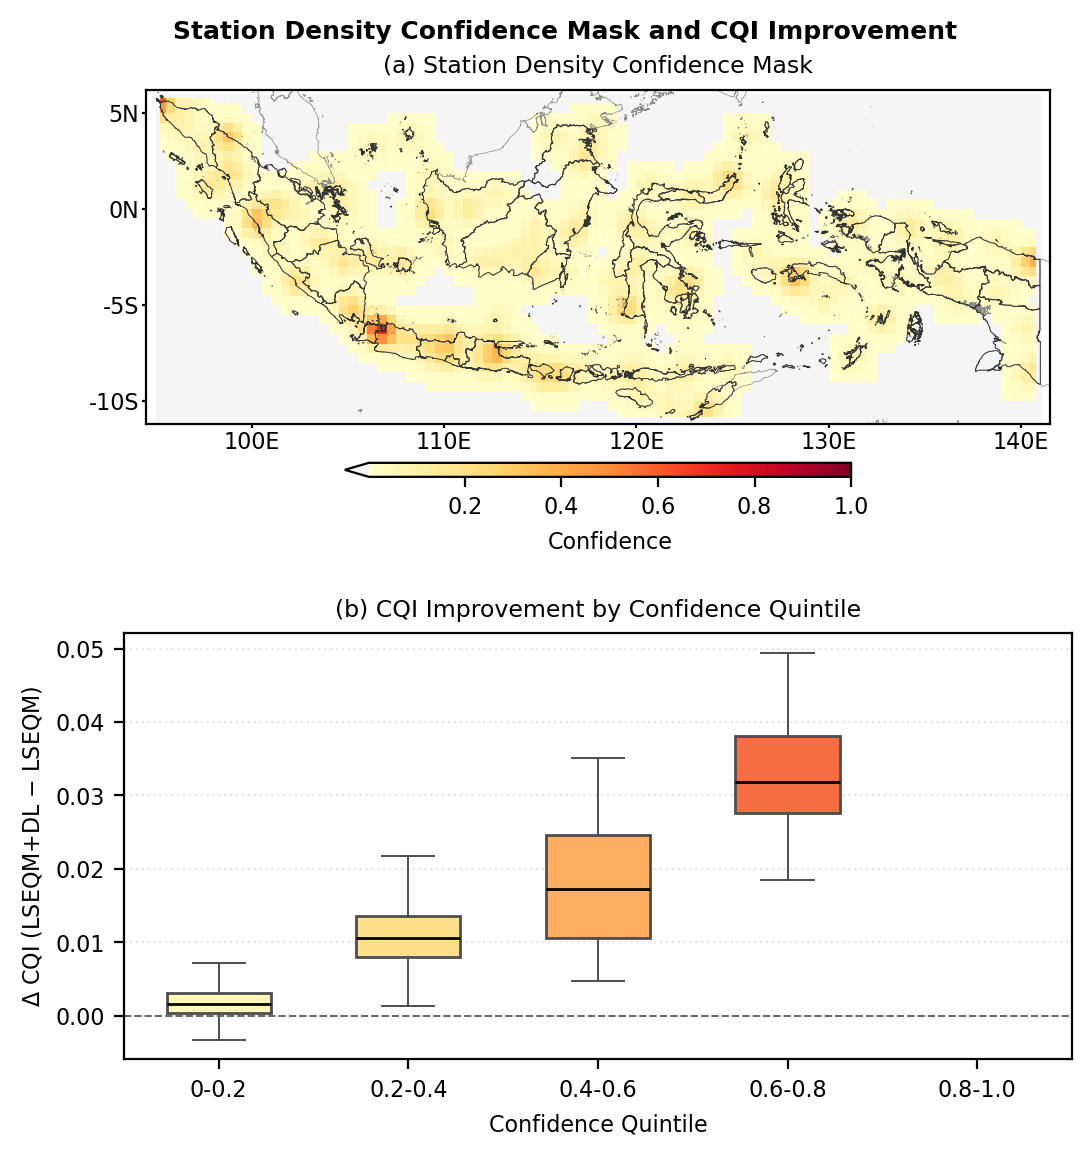
\includegraphics[width=\figFiveThreeWidth\textwidth]{fig_thesis_05_confidence_mask.png}
\caption[Station-density confidence mask]{Station-density confidence mask\label{fig:confmask}}
\end{figure}

The fourth category combines comparison studies and training
use. The notebook structure separates correction from
verification, so the four-pillar verification report can be run
on any pair of satellite and reference fields without re-running
the correction. This lets independent groups compare IMERG Final
Run against IMERG Late Run, or a bias-corrected output from a
different pipeline against the same BMKG validation set, against
a numerically comparable baseline. The same structure, combined
with the free-tier Colab runtime in the order of minutes per
dekad, supports use as a graduate-level training resource on
satellite precipitation bias correction
\citep{ref:perkel2018, ref:wagemann2022}. This is not the central
scientific contribution of the present work, but it is a
substantive secondary benefit of the open release.

The reproducibility contribution carries its own limitations,
which Section~\ref{sec:discussion-limitations} catalogues. The
pinned dependency versions will drift, the Colab environment will
evolve, and the input data archives at the National Aeronautics
and Space Administration (NASA) Goddard Earth Sciences Data and
Information Services Center (GES DISC) and National Oceanic and
Atmospheric Administration (NOAA) CPC have their own retention and
re-processing policies that the
present work cannot control. The reproducibility claim is
therefore scoped: it holds against the specific versions and
archive states recorded at the time of release, and it requires
the dependency snapshot to be maintained for the verification
exercise to remain reproducible in the long term. The discussion
returns to this scope in Section~\ref{sec:discussion-limitations}.


% ============================================================
\section{Paths Forward}\label{sec:discussion-paths}
% ============================================================

Raising the temporal-skill ceiling beyond $r \approx 0.35$
requires methods outside the marginal correction family. This
section surveys four paths and assesses their feasibility for the
Indonesian domain, the data products available, and the
infrastructure costs they impose on operational users. The order
reflects increasing methodological distance from the present
pipeline. Table~\ref{tab:paths-forward} summarises the four
paths against three criteria: the methodological distance from
the LSEQM+DL pipeline, the infrastructure cost they impose, and
their effect on the temporal-skill ceiling for the Maritime
Continent setting.

\begin{table}[H]
\centering
\caption[Four paths for raising the temporal-skill ceiling beyond $r \approx 0.35$]{Four paths for raising the temporal-skill ceiling
beyond $r \approx 0.35$\label{tab:paths-forward}}
\begingroup\small
% Use tabular* so the table fills \textwidth exactly: keep the original
% 3.0/2.0/2.5/4.5 cm p-column widths (sum 12 cm) and let
% \extracolsep{\fill} absorb the ~2 cm of slack into the inter-column
% gaps. Previous attempt scaled the p widths to 14 cm but forgot the
% three 12 pt inter-column paddings (~1.3 cm), pushing the table past
% the right margin.
\begin{tabular*}{\textwidth}{@{\extracolsep{\fill}}p{3.0cm}p{2.0cm}p{2.5cm}p{4.5cm}@{}}
\toprule
Path & Methodological distance & Infrastructure cost & Ceiling effect \\
\midrule
Multivariate QM &
Moderate (replace univariate marginal with joint mapping) &
Larger calibration samples; tens of times more compute &
Open question; depends on joint structure of the reference \\
\addlinespace
Sub-daily disaggregation &
Moderate (add a step after daily correction) &
Half-hourly archive + geostationary IR &
Moderate; recovers within-day timing only \\
\addlinespace
Stochastic disaggregation &
Large (deterministic $\to$ ensemble) &
Ensemble verification stack on the downstream side &
Reframes timing as uncertainty rather than removing it \\
\addlinespace
Local-day re-aggregation (with Himawari-9) &
Small (re-aggregate input before pipeline) &
Re-run of pipeline on re-aggregated archive &
Targets the UTC-vs-local-day calendar artefact; most actionable for UTC+7--9 \\
\bottomrule
\end{tabular*}
\endgroup
\end{table}

The first path is multivariate quantile mapping. The univariate
methods used throughout the present pipeline correct the marginal
distribution at each pixel and each dekad independently.
Multivariate methods correct the joint distribution across pixels,
across pairs of variables, or across time lags, and can in
principle restore some of the day-by-day pairing that the
univariate methods leave untouched. The rank preservation
argument of Section~\ref{sec:discussion-bound} is specifically a
property of marginal mapping, so a multivariate method is not
bound by it. The trade-off is that multivariate methods require
substantially larger calibration samples and substantially more
computation, and the quality of the joint structure they recover
is bounded by the joint structure of the calibration reference.
For a regional pipeline calibrated against a $0.5^{\circ}$ gauge
analysis with $172$ validation stations, the joint structure
recoverable is limited, and the gain in temporal skill that a
multivariate method can deliver in this setting is an open
question that the present work does not resolve.

The second path is sub-daily disaggregation. The IMERG product
family is natively half-hourly, and the daily aggregation step
applied in the present pipeline discards the within-day timing
information. Sub-daily disaggregation, in which the corrected
daily total is redistributed across the day using a
cloud-tracking algorithm against half-hourly imagery, recovers
the within-day timing at the cost of additional dependencies on
geostationary infrared and visible channels. For the Maritime
Continent, the Himawari-9 geostationary platform~\citep{ref:bessho2016} provides
$10$-minute cadence at $2$~km resolution and is the natural
candidate for the cloud-tracking input. This path retains the
distributional correction at the daily scale and adds a
within-day timing signal on top, so the bias-free distributional
properties of the present pipeline are preserved while the
day-by-day timing is recovered.

The third path is stochastic disaggregation. Rather than
producing a single corrected daily field, a stochastic
disaggregation step samples from an ensemble of plausible daily
timings consistent with the corrected distributional properties.
The verification posture shifts from deterministic point-by-point
scoring to ensemble metrics: the Continuous Ranked Probability
Score for ensembles, the rank histogram for calibration, and
threshold reliability diagrams for event detection~\citep{ref:wilks2020}. The path is
attractive because it acknowledges the timing uncertainty
explicitly rather than burying it in a flat $r$ value. The cost
is that downstream operational users need to ingest ensemble
inputs, which not all hydrological models or drought-monitoring
applications are equipped to handle. The path is therefore most
useful for applications that are already ensemble-aware.

The fourth path, and the most operationally actionable for users
in the UTC+7 to UTC+9 band, is morning-observation re-aggregation
of the daily IMERG-L archive. The calendar-window mismatch
diagnosed in Section~\ref{sec:discussion-subdaily} places the
optimal alignment at $h \approx -23$~h relative to UTC midnight,
matching the date label the BMKG validation network assigns under
its morning-observation convention \citep{ref:bmkg2006sk32}. The
CPC-UNI calibration target needs no such shift: it is already
dated to the UTC day and peaks at $h \approx 0$
\citep{ref:cpcuni_readme}. Re-aggregating the native half-hourly
IMERG fields \citep{ref:imerghhl07} to a 24-hour window ending at
$07{:}00$ local time on the recorded date, before applying the
LSEQM+DL correction, would remove the mismatch component without
changing the correction methodology.

The expected operational
effect, from the diagnostic in
Section~\ref{sec:discussion-subdaily}, is a lift in the GPM-era
daily Pearson $r$ against BMKG, pooled over all station-days, from
approximately $0.20$ at the
UTC-day window to approximately $0.57$ at the matched window. The
four-pillar corrections apply unchanged, and their value,
distribution, extreme, and detection scores are recomputed on the
re-aggregated daily totals and expected to remain close. The cost is a re-run
of the entire pipeline against a re-aggregated input archive,
which is computationally modest but archive-intensive. This is
the path most directly enabled by the parallel reproducibility
contribution: the configurable daily-aggregation step is exposed
in the pipeline, the re-aggregated archive can be substituted at
the input layer, and the four-pillar verification report on the
re-aggregated pipeline against the same BMKG validation set is
reproducible by any independent user.

A common feature of all four paths is that they leave the
LSEQM+DL pipeline as constructed in Chapter~\ref{chap:methods}
intact for the well-served application class identified in
Section~\ref{sec:discussion-ops}. Users who do not need
day-specific timing receive the corrected daily product as is;
users who need timing receive an upstream re-aggregation, an
add-on disaggregation, or a shift to an ensemble representation.
The marginal correction component remains the right tool for the
distribution-alignment work, and the four paths above add
capability rather than replace existing capability.


% ============================================================
\section{Limitations and Constraints}\label{sec:discussion-limitations}
% ============================================================

The present work has six limitations that bound the strength of
its conclusions. They are catalogued here so that the
operational guidance in Section~\ref{sec:discussion-ops} and the
reproducibility claim in
Section~\ref{sec:discussion-reproducibility} can be read at the
right level of confidence.

\textbf{Sensitivity parameters not formally optimised.} Three
parameters in the pipeline carry the not-formally-optimised
status declared in Section~\ref{sec:methods-reproducibility}: the
CNN blending weight $\alpha = 0.70$, the GPD threshold at the
$80$th percentile of wet-day exceedances, and the density
saturation count at $2$ (lowered from an initial $3$ after
qualitative inspection showed that $3$ suppressed the CNN almost
everywhere outside Java). Each was chosen by domain reasoning,
each is exposed in the configuration file, and each is acknowledged
as a sensitivity parameter rather than an optimum. The headline
numbers in Chapter~\ref{chap:results} are conditional on these
choices. A one-at-a-time sweep over five values per parameter on
the Bali reproducibility subdomain
(Section~\ref{sec:results-sensitivity}) confirms that each
parameter response is monotone and locally smooth and that the
four-pillar pattern does not reverse across the explored ranges; a
full Cartesian grid search with a strict temporal hold-out remains
future work. Users who care about the precise headline value
should re-run the pipeline with their own preferred settings;
users who care about the four-pillar pattern can rely on its
stability across the Bali sweep, which is a single-subdomain test.

\textbf{CPC-UNI reference quality bound.} The framework
calibrates against CPC-UNI, whose known undercatch of heavy
rainfall and $0.5^{\circ}$ interpolation smoothing bound the
reference quality. Section~\ref{sec:methods-reference-quality}
traces both to their source: the Indonesian input reaches CPC
through the routine GTS exchange rather than the full national
network, and that input is drawn from an archive missing a third
of its station-days, so the reference is well constrained where
the contributing network is dense and progressively less so where
it thins. The
corrected satellite product cannot be
better than the reference it is calibrated against, except where
the BMKG out-of-sample validation reveals that the corrected
product matches the BMKG distribution more closely than CPC-UNI
does, as discussed in Section~\ref{sec:results-headline}. The
strongest claim the present work supports is that the corrected
product is bias-free at the four pillars when scored against an
independent gauge network, conditional on the CPC-UNI reference
defining the correction target. Replacement of CPC-UNI by a
higher-resolution or denser-gauge analysis remains an extension
within the same pipeline architecture.

\textbf{CNN training-data limits at the network edges.} The CNN
refinement stage uses dekadal pooling of approximately $250$
paired daily observations per pixel over $25$ years. In regions
of very sparse gauge coverage, the station-density confidence
mask formula in Section~\ref{sec:methods-blending} drives
$\alpha_{\text{eff}}$ toward $1$, which restricts the CNN
contribution to areas where the calibration sample is large
enough to support the residual learning target. This is graceful
degradation rather than failure: in low-confidence regions the
pipeline collapses to LSEQM, and the four-pillar performance in
those regions is the LSEQM column of Table~\ref{tab:headline}
rather than the LSEQM+DL column. The implication for users in
Papua and parts of Maluku is that the headline LSEQM+DL numbers
do not apply uniformly across the archipelago; in those regions
the LSEQM column of Table~\ref{tab:headline} is the relevant
performance baseline.

\textbf{Conditional bias not removable by univariate quantile
mapping.} The Pearson $r$ ceiling discussed in
Section~\ref{sec:discussion-bound} is one expression of a more
general limit: conditional biases, in which the satellite error
depends on the precipitation amount in a way that the univariate
mapping cannot capture, are not removable by the present
pipeline. The four paths in Section~\ref{sec:discussion-paths}
all address this limit at different points in the pipeline. The
present work does not claim to remove conditional bias; it
claims to remove the marginal bias and to acknowledge the
conditional component as the structural ceiling.

\textbf{Calendar-window mismatch between IMERG-L and the gauge
reference family.} The daily IMERG-L archive is constructed on
the UTC calendar day. CPC-UNI shares that date label, closing each
total at $00{:}00$~UTC \citep{ref:cpcuni_readme}, whereas the BMKG
network dates its totals to the local day ending at the morning
observation \citep{ref:bmkg2006sk32}, a mismatch of approximately
$23$~hours per the diagnostic in
Section~\ref{sec:discussion-subdaily}. The mismatch therefore
arises only at the validation end, not at the calibration end. The four-pillar results
(value, distribution, extreme, detection) are unaffected, being
functions of the marginal distribution and of categorical events
that are invariant to the 24-hour window choice; only Pearson~$r$
against the BMKG validation gauges is suppressed by the label
offset, and it is recovered by re-aggregating the satellite to the
local-observation day, identified as the most operationally
actionable path forward (Section~\ref{sec:discussion-paths}).

\textbf{Reproducibility scope is version-bounded.} The
dependencies pinned at release time will drift as the Python
ecosystem evolves and as cloud-platform defaults change. The
reproducibility claim is therefore scoped to the dependency
snapshot recorded in the requirements file at release. A long-term
reproducibility commitment requires either a containerised
distribution (which the present release does not provide) or an
ongoing maintenance commitment to track upstream changes (which
the present author cannot offer beyond the thesis defence
horizon). The verification exercises that
Section~\ref{sec:discussion-reproducibility} discusses should
therefore be undertaken with the recorded dependency snapshot,
not with a current environment, until a containerised release is
prepared.

The combined effect of these six limitations leaves the central
claim of the chapter intact: marginal bias correction moves the
four pillars cleanly toward the gauge target but does not improve
the temporal-skill diagnostics beyond single-pixel sampling noise,
because rank preservation and variance inflation without skill hold
Pearson $r$ near the timing quality of the underlying satellite
retrieval. The four-pillar
improvement is the contribution that the framework delivers; the
flat $r$ is the structural property of the method family rather
than a failure of the implementation. The reproducibility
contribution lowers the cost of testing this proposition on other
products, other references, and other regions; the transferability
of the proposition itself is an empirical question that the open
release lets the field answer one re-application at a time.
Chapter~\ref{chap:conclusion} draws these threads together, states
what the framework does and does not deliver against the objectives
and hypotheses of Chapter~\ref{chap:introduction}, and sets out the
recommendations that follow for users,
for researchers extending the method, and for the institutions that
maintain the underlying archives.

% ============================================================
% chapter_06_conclusion.tex - Chapter 6, Conclusion
%
% Purpose: summarises the empirical findings, the methodological
%          finding (full reproducibility on free cloud infrastructure),
%          and the recommendations for the wider research community.
% Sections: 6.1 Summary of Findings, 6.2 Implications,
%           6.3 Recommendations.
% Included by main_thesis.tex.
% License: CC BY 4.0 (see ../LICENSE).
% ============================================================

\chapter{CONCLUSION}\label{chap:conclusion}

This thesis set out to present a hybrid bias correction framework
for daily satellite precipitation and to establish, dimension by
dimension, what it corrects and where it is bounded. It delivered
the result in two registers: what the framework achieves as a
scientific result, and what it provides as a reproducible
methodological artefact. This chapter summarises
the findings, states their implications, and sets out
recommendations for users, researchers, and the institutions that
maintain the underlying data.


% ============================================================
\section{Summary of Findings}\label{sec:conclusion-summary}
% ============================================================

The scientific finding is a stage-resolved account of what the
LSEQM+DL (Linear Scaling, Empirical Quantile Mapping, Generalized
Pareto Distribution tail correction, and Deep Learning refinement
through a Convolutional Neural Network) framework corrects and
what it leaves unmoved. Applied to the Integrated Multi-satellitE Retrievals for the
Global Precipitation Measurement (GPM) mission (IMERG) Late Run
(IMERG-L) over Indonesia across 2001 to 2025 and validated against
172 independent Indonesian Meteorological, Climatological, and
Geophysical Agency (BMKG) stations over 2001 to 2021, the pipeline moves three
of the four verification pillars cleanly toward the gauge target.

The value-adjustment
pillar reaches a relative bias near zero and a standard deviation
ratio of unity; the distribution-alignment pillar reaches a
Kolmogorov-Smirnov $p$-value at which the corrected and gauge
distributions are no longer statistically distinguishable; and
the extreme-preservation pillar reaches $Q_{99}$ within one
percent of the gauge target. The fourth pillar, event detection,
shows a designed trade-off: the aggregate probability of
detection falls as the dry-day-matching mechanism suppresses
spurious light rain. The threshold-stratified view, however, shows the
LSEQM+DL pipeline overtaking Linear Scaling at and above the
$20$~mm/day very-heavy-precipitation threshold of the
internationally standardised extremes indices.
Each stage moves the metrics matched to its design dimension and
leaves the others alone.

The most consequential result is the one metric that
does not move. Measured per pixel against the CPC-UNI calibration
target, the Pearson correlation between paired daily values stays
near $0.35$ across all three corrected stages, a shift smaller
than the single-pixel sampling uncertainty. The same flat pattern
holds against the independent BMKG stations, station-by-station in
the Taylor analysis and month-by-month across the seasonal cycle,
and it survives the correction of the calendar-window offset
(Section~\ref{sec:results-intercomparison}). This is not a failure of the implementation. It is the
predicted behaviour of any marginal correction family: rank
preservation and variance inflation without time-dependent skill
together leave the daily correlation set by the day-by-day
pairing quality of the raw satellite retrieval, which lies
upstream of every step in the pipeline.

The corrected
in-sample value of $0.348$ against CPC-UNI is of the order reported
for daily IMERG over the Indonesian Maritime Continent
\citep{ref:ramadhan2022ts}, and well below the median near $0.75$
the same product reaches against the far denser Chinese gauge
analysis \citep{ref:tang2020}; the calendar-window diagnostic
accounts for most of that difference. The framework's reach is
therefore precise: a marginal-correction framework
can take a daily field all the way to the gauge marginal
distribution at every percentile, and no distance at all along
the axis of day-by-day timing.

These results resolve the three hypotheses of
Section~\ref{sec:intro-hypotheses}. H1 is supported: each stage
moves its matched pillar toward the gauge target, with the
Convolutional Neural Network acting as a small, spatially targeted
refinement of the extreme tail
(Section~\ref{sec:results-stages}). H2 is supported against both
references and at both date labels: the daily correlation does not
improve beyond the sampling uncertainty across the corrected
stages, against the in-sample CPC-UNI target and the independent
BMKG stations alike. H3 holds in the GPM era: the low daily
correlation against BMKG is substantially a calendar-label
artifact, recoverable by matching the satellite to the gauge day,
and the recovery is specific to the era in which the retrieval
resolves the diurnal cycle.

The methodological finding is that this entire account is
independently reproducible. The pipeline is released as a
configuration-driven set of source modules and numbered
notebooks that run unchanged in a local environment or on a
free-tier cloud instance. The correction-to-visualisation sequence
was re-executed
on a free Google Colab instance for the Bali subdomain across all
36 dekadal windows in 72.1 minutes on a standard Central
Processing Unit (CPU) runtime. That establishes that an independent
reader can reconstruct the results for a self-contained region
without institutional compute access; the full Indonesian domain
scales up with pixel count and is correspondingly longer. The two findings are of equal
weight: the scientific result is credible because it is
reproducible, and the reproducible artefact is worth releasing
because it carries a result worth re-verifying.


% ============================================================
\section{Implications}\label{sec:conclusion-implications}
% ============================================================

For operational use, the central implication is that the
corrected product should be matched to the metrics that moved.
The corrected daily IMERG-L is suitable for the broad class of
applications that depend on distributional properties:
dekadal-to-monthly water budgets, drought indicators such as the
Standardized Precipitation Index and its evapotranspiration
variant, extreme-event frequency analysis, threshold-exceedance
climatology, and hydrological model calibration against multi-year
statistics. It is not suitable, on its own, for applications that
depend on the precise calendar day of an event: real-time
flood-event nowcasting, single-event forecasting, and day-1
hydrological initialisation inherit the timing ceiling of the raw
retrieval and must combine the corrected product with sub-daily
disaggregation, move to ensemble methods, or accept the timing
limitation. Correcting at the daily scale remains necessary so
that the dekadal, monthly, and seasonal aggregates derived from
the daily field are bias-free.

For the open-science contribution, the implication is that the
verification posture argued for in this thesis can be applied by
others. The four-pillar framework with Pearson correlation
reported as a separate temporal-skill diagnostic, rather than
folded into a single skill score, lets a structural limit and a
methodological improvement appear in the same report. An
independent group can apply the same verification scaffolding to
a different product, a different reference, or a different region,
and can reproduce or challenge the present result on its own
terms.


% ============================================================
\section{Recommendations}\label{sec:conclusion-recommendations}
% ============================================================

\medskip\noindent\textbf{For users of corrected satellite
precipitation.}
Read the verification report before choosing an application.
A product that matches the gauge distribution is the right input
for distributional questions and the wrong input for
day-specific timing questions, and the two cases cannot be told
apart from an aggregate skill score alone. Where the application
is timing-sensitive and operates over the Maritime Continent, do
not reject the product on its daily correlation before checking
the calendar: the UTC-aligned daily window is a known contributor
to the timing ceiling, and the recovery available from a
locally-aligned re-aggregation, quantified in
Section~\ref{sec:discussion-subdaily}, costs nothing elsewhere in
the pipeline.

\medskip\noindent\textbf{For researchers extending the method.}
Start with the calendar window. Of the four extensions set out in
Section~\ref{sec:discussion-paths}, re-aggregating the daily
archive to the local-observation window is the only one that
leaves the pipeline untouched, and it addresses the larger of the
two components of the timing ceiling. The remaining three, which
reach the residual retrieval-skill component, all require methods
outside the marginal correction family and are correspondingly
more costly. Three further extensions are worth stating as
recommendations rather than as findings: a joint search over the
three sensitivity parameters with a strict temporal hold-out,
which this study explored only one parameter at a time; a
transfer experiment to a second tropical region, which would test
a portability the framework's design allows but does not
establish; and the fully-convolutional Stage~4 head described in
Section~\ref{sec:methods-cnn}, which matched the dense model on
the Bali subdomain at a fraction of the parameter count and is
the natural replacement at full resolution.

\medskip\noindent\textbf{For BMKG, CPC, and Institut Pertanian Bogor (IPB).}
The reproducibility contribution depends on continued access to
the underlying archives and on the maintenance of the released
code against dependency drift. A containerised distribution and a
versioned data snapshot would make the reproducibility claim
durable beyond the dependency state recorded at release. More
broadly, the gap this thesis addresses, namely the rarity of
released code in the bias correction literature, is one that
institutional data-sharing and reproducibility standards are well
placed to close, and the framework released here is offered as a
concrete example of what such standards can produce.


% --- References ---
\cleardoublepage
\phantomsection
\addcontentsline{toc}{chapter}{REFERENCES}
\ifAPAcite
  \bibliographystyle{ipb}        % IPB English author-year (./ipb.bst)
\else
  \bibliographystyle{unsrtnat}   % MDPI numeric, natbib-compatible
\fi
\bibliography{references}

% --- Appendices ---
% ============================================================
% chapter_99_appendices.tex - Appendices A through H
%
% Purpose: archival back-matter material kept separate from the body
%          chapters: data sources, code+data availability, full
%          configuration template, per-station verification table,
%          reproducibility checklist, glossary, and the spatial atlas.
% Sections: A Data Catalogue, B Code and Data Availability,
%           C Configuration Template, D Per-Station Verification,
%           E Reproducibility Checklist, F Glossary, G Spatial Atlas,
%           H Supplementary Temporal-Alignment Diagnostics.
% Numbering: \thefigure / \thetable / \theequation prefix re-set to
%            the appendix letter so figures land as G.1, G.2, ...
%            instead of clashing with the Chapter 4 numbering.
% Included by main_thesis.tex (after Chapter 6).
% License: CC BY 4.0 (see ../LICENSE).
% ============================================================

% ----- APPENDICES divider: title at top of page -----
\clearpage
\thispagestyle{fancy}
\begin{center}
  {\fontsize{14}{17}\selectfont\bfseries APPENDICES}
\end{center}
\addcontentsline{toc}{chapter}{APPENDICES}
\vspace{\baselineskip}

\appendix
% In the appendix the chapter counter restarts; the body-chapter numbering
% scheme would produce table/figure numbers like "4.1" (chapter 4 ==
% Appendix D), colliding with Chapter 4. Switch the prefix to the appendix
% letter so the first table in Appendix D becomes "D.1" and the list of
% tables/figures shows letters rather than digits.
\renewcommand{\thetable}{\Alph{chapter}.\arabic{table}}
\renewcommand{\thefigure}{\Alph{chapter}.\arabic{figure}}
\renewcommand{\theequation}{\Alph{chapter}.\arabic{equation}}
% Make the appendices flow continuously: remove the forced page break that
% \chapter normally issues, so each appendix follows the previous one on the
% same page (a new page is taken only when the content runs over). This patch
% is applied here, after the main chapters, so only appendices A-F are
% affected; the biography uses its own explicit \clearpage.
\makeatletter
\patchcmd{\chapter}{\if@openright\cleardoublepage\else\clearpage\fi}{}{}{}
\makeatother
% Appendix chapter headings: left-aligned, "A. DATA CATALOGUE" (heading 1).
\titleformat{\chapter}[hang]
  {\normalfont\fontsize{14}{17}\selectfont\bfseries}
  {\thechapter.}{0.6em}{\MakeUppercase}
\titlespacing*{\chapter}{0pt}{1.5\baselineskip}{6pt}

% ============================================================
\chapter{Data Catalogue}\label{app:data}
\addcontentsline{apx}{appx}{\protect\numberline{Appendix~\thechapter}Data Catalogue}
% ============================================================

\section{Datasets}

The study uses three precipitation datasets and one validation
network. Acronyms used across the appendices follow the same usage
as the main chapters and are summarised inline at first use here.
The Integrated Multi-satellitE Retrievals for Global Precipitation
Measurement (GPM) Late Run (IMERG-L, V07, $0.1^{\circ}$,
approximately 14-hour latency) is the satellite product corrected
\citep{ref:huffman2020}. The IMERG Final Run (IMERG-F, V07,
$0.1^{\circ}$) is retained as an independent benchmark but is not
used in the correction. The Climate Prediction Center (CPC)
Unified Gauge-Based Analysis of Global Daily Precipitation
(CPC-UNI, $0.5^{\circ}$) is the correction reference
\citep{ref:chen2008}. Satellite data were obtained from the
National Aeronautics and Space Administration (NASA) Goddard Earth
Sciences Data and Information Services Center (GES DISC); CPC-UNI
from the National Oceanic and Atmospheric Administration (NOAA)
Physical Sciences Laboratory. All fields span 2001 to 2025 and are
processed per dekad (days 1 to 10, 11 to 20, 21 to month end).

\section{BMKG validation network: 180 to 172}

Independent validation uses daily station observations from
Indonesia's Meteorological, Climatological, and Geophysical Agency
(BMKG). The parent network has approximately 180 stations; two
filters reduce it to the 172 used in validation:

\begin{enumerate}
    \item \textbf{Spatial-mapping filter.} The station coordinates
    must fall within the land mask used by the satellite product.
    A small number of stations near the maritime border or with
    mis-recorded coordinates fail this test.
    \item \textbf{Minimum paired-day filter.} After sentinel
    removal and pairing against the corrected satellite series,
    the station must retain at least \texttt{MIN\_VALID\_DAYS}
    (approximately 30) paired daily observations per dekadal
    window.
\end{enumerate}

Together these drop 8 of 180 stations, leaving 172 for the
per-station Taylor diagrams, multi-threshold verification, and
station-level summaries.

\section{Sentinel handling}

The BMKG archive encodes missing data with the sentinel value
$8888$. Across the raw record this sentinel occurs $76{,}778$
times ($8.02\%$ of raw cells); leaving it unfiltered would inflate
heavy-threshold event counts catastrophically (by more than
$1000\%$ at the $100$~mm/day threshold, because every sentinel
exceeds every physical threshold). The loader removes the sentinel
through the centralised \texttt{MISSING\_SENTINEL} configuration
value before any analysis, leaving $880{,}702$ valid daily
observations with a maximum physical daily total of $1{,}965.5$~mm.
All threshold-based verification in this thesis uses the
sentinel-filtered observations. A different station archive with a
different sentinel convention (for example $9999$ or $-999$) would
require the sentinel value to be reset in the configuration.


% ============================================================
\chapter{Code and Data Availability}\label{app:code}
\addcontentsline{apx}{appx}{\protect\numberline{Appendix~\thechapter}Code and Data Availability}
% ============================================================

The framework is released as an open implementation. The source
code, the six numbered notebooks, and the Quarto documentation
site are hosted on GitHub at
\url{https://github.com/bennyistanto/hybrid-bias-correction}
under the Mozilla Public License 2.0. The notebooks open directly
in Google Colab from the repository, and a province-scale Bali
example dataset is bundled in the repository so the pipeline can be
run without any external download.

The full Indonesia operational inputs (IMERG, CPC, and BMKG for
2001 to 2025, approximately $1.7$~GB) and the complete outputs
(corrected NetCDFs, metrics, quality assessment, station
validation, and figures, approximately $40$~GB) are deposited on
Zenodo with a citable DOI:
\url{https://doi.org/10.5281/zenodo.20287847}. To reproduce the
Indonesia results, a reader clones the repository, downloads the
Zenodo bundle, points \texttt{config.yml} at the extracted
directories, and runs the notebooks. The companion manuscript is
under review at \emph{Remote Sensing} (MDPI)\MDPIstatus; its DOI
and citation will be added on acceptance.


% ============================================================
\chapter{Configuration Template}\label{app:config}
\addcontentsline{apx}{appx}{\protect\numberline{Appendix~\thechapter}Configuration Template}
% ============================================================

The pipeline is driven by a single \texttt{config.yml} file that
resolves environment placeholders (\texttt{\{main\_dir\}},
\texttt{\{input\_dir\}}, \texttt{\{output\_dir\}}) at load time.
The annotated excerpt below shows the parameters most relevant to
this thesis; the full file is in the repository.

{\footnotesize
\begin{verbatim}
# --- Area of interest (Bali example subdomain) ---
aoi:
  lat_range: [-8.85, -8.05]
  lon_range: [114.45, 115.75]
# --- Distribution fitting ---
statistics:
  gpd_threshold_percentile: 80   # GPD tail threshold (wet-day pctl)
# --- Deep learning blend ---
deep_learning:
  blend_alpha: 0.70              # LSEQM weight at full confidence
  use_confidence_mask: true
# --- Station-density confidence mask ---
station_density:
  saturation_count: 2            # gauges per CPC cell for full confidence
  smoothing_sigma: 1.0
# --- Quality assessment (CQI component weights) ---
quality_assessment:
  component_weights:
    basic_stats: 0.4
    distribution: 0.3
    temporal: 0.3
\end{verbatim}
}

\enlargethispage{\baselineskip}%   keep the short closing paragraph on the same page as the verbatim
The three sensitivity parameters identified in
Chapter~\ref{chap:methods} (\texttt{blend\_alpha},
\texttt{gpd\_threshold\_percentile}, \texttt{saturation\_count})
are all set here, which is what makes the sensitivity sweep of
Section~\ref{sec:results-sensitivity} a configuration change 
rather than a code change.


% ============================================================
\chapter{Selected Per-Station Verification}\label{app:stations}
\addcontentsline{apx}{appx}{\protect\numberline{Appendix~\thechapter}Selected Per-Station Verification}
% ============================================================

Table~\ref{tab:perstation-bali} reports the per-station Taylor
statistics for the four BMKG stations on Bali, computed against
the daily station records over 2001 to 2021. The table illustrates
the correlation pattern at the level of individual stations: the
Pearson correlation barely moves between the raw IMERG-L and the
corrected LSEQM+DL series, while the standard deviation of the
corrected series moves toward the observed standard deviation. The
single-station daily samples are smaller and noisier than the
pooled 172-station Indonesia result, but the same pattern is
visible. The full per-station tables for all 172 Indonesia
stations are in the Zenodo release.
Table~\ref{tab:perstation-bali} reports, per station, the correlation
($r$) against the daily station record for raw IMERG-L and corrected
LSEQM+DL, the observed and LSEQM+DL standard deviations ($\sigma$, in
mm/day), and the LSEQM+DL bias (mm/day).

\begin{table}[H]
\centering
\caption{Per-station Taylor statistics for the four Bali BMKG stations.\label{tab:perstation-bali}}
\begingroup\small
\begin{tabular}{@{}lccccc@{}}
\toprule
Station (WMO ID) & $r$ IMERG-L & $r$ LSEQM+DL & $\sigma_{\text{obs}}$ & $\sigma_{\text{LSEQM+DL}}$ & Bias \\
\midrule
Ngurah Rai (97230)   & 0.387 & 0.388 & 14.08 & 14.32 & $+0.13$ \\
Denpasar (97232)     & 0.387 & 0.390 & 17.17 & 15.37 & $-0.73$ \\
Kahang-Kahang (97234)& 0.286 & 0.268 & 14.42 & 12.58 & $-0.47$ \\
Jembrana (97236)     & 0.233 & 0.202 & 17.36 & 11.52 & $-2.54$ \\
\bottomrule
\end{tabular}
\endgroup
\end{table}

\medskip
The single-month noise in such per-station figures is large enough to be
worth quantifying, because the optimal-window analysis of
Section~\ref{sec:results-window} reports per-station correlations, and an
earlier single-month version of that analysis produced systematically
larger per-station values. Figure~\ref{fig:noise-selection} explains the
difference. A per-station correlation estimated from a single month rests
on roughly ten to twenty wet days, so it scatters widely around its true
value: at a fixed aggregation window the single-month estimate has a
median near the seven-year value (both near $0.56$) but an
interquartile range of $[0.35, 0.73]$. Taking the maximum over the $97$
candidate window offsets then adds a selection bias, shifting the
single-month median up to $0.66$ and inflating the high tail, so that
half the stations appear to exceed $r = 0.65$. Both effects vanish on the
full seven-year record, where each offset is estimated precisely: the
per-station peak correlation tightens to a median of $0.56$ with an
interquartile range of $[0.51, 0.62]$, and the selection bias disappears
because the peak and fixed-window values coincide. The per-station
figures reported in the main text use the seven-year estimates for this
reason.

\begin{figure}[H]
\centering
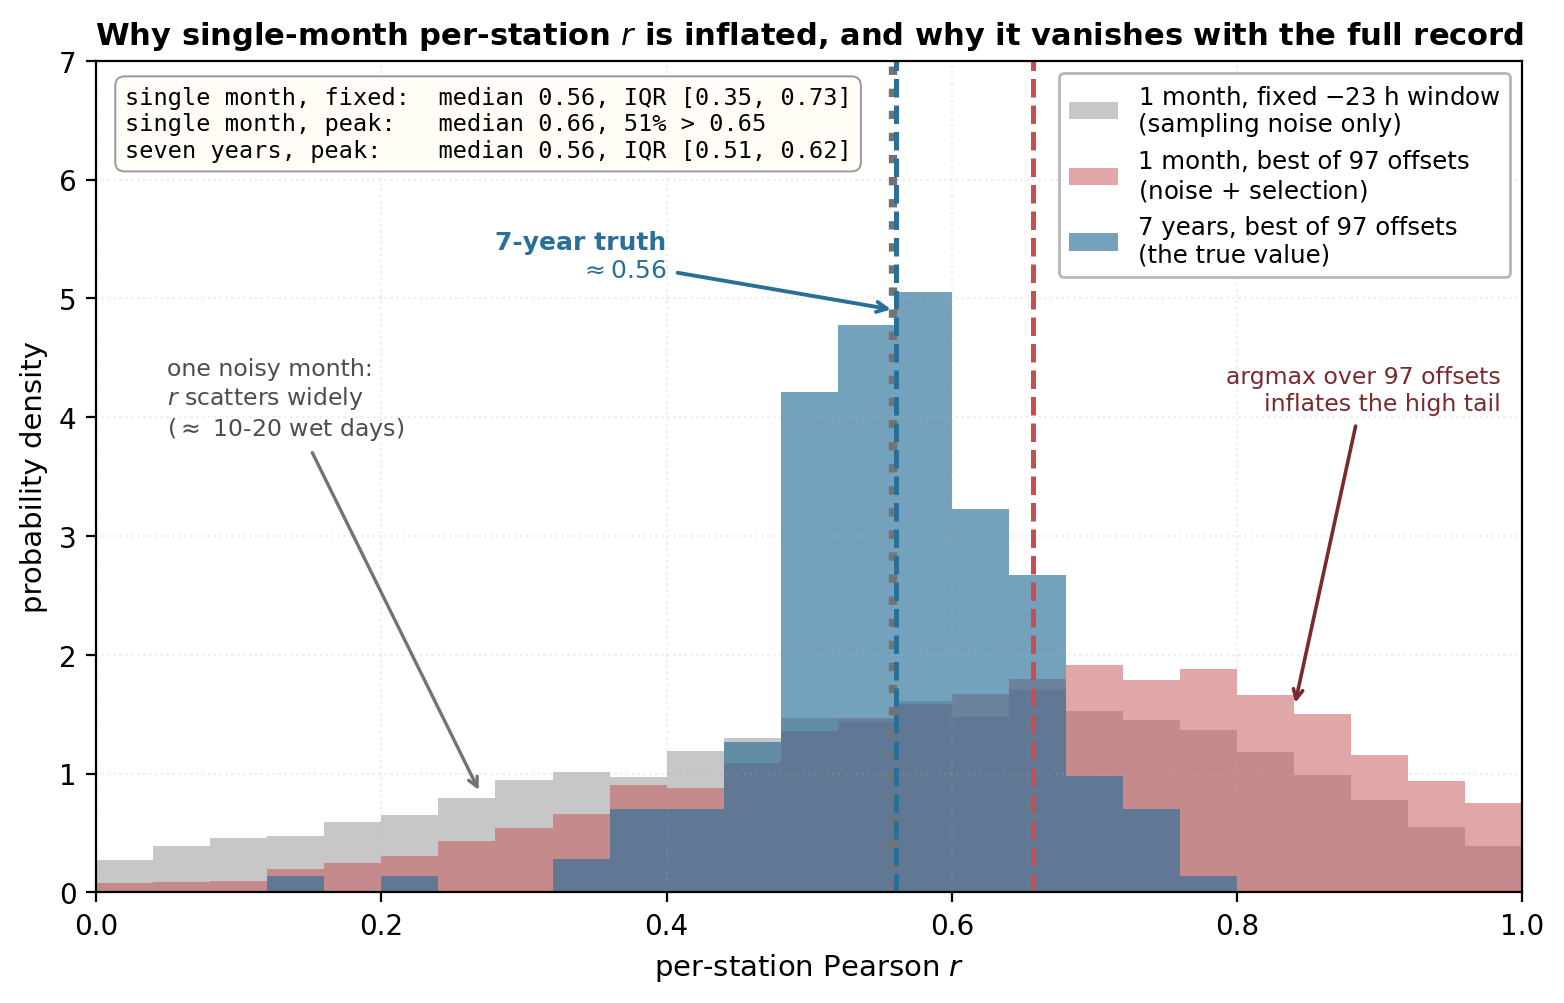
\includegraphics[width=\textwidth]{fig_thesis_99_noise_selection.png}
\caption[Sampling stability of the per-station window correlation]{Sampling
stability of the per-station window correlation: one month is inflated by
noise and offset selection, the seven-year record is precise (dashed lines
mark each distribution's median).\label{fig:noise-selection}}
\end{figure}


% ============================================================
\chapter{Reproducibility Checklist}\label{app:repro}
\addcontentsline{apx}{appx}{\protect\numberline{Appendix~\thechapter}Reproducibility Checklist}
% ============================================================

This checklist records what an independent reader needs in order
to reproduce the results, following the reproducibility design of
Section~\ref{sec:methods-reproducibility} and the empirical
evaluation of Section~\ref{sec:results-reproducibility}.

\medskip\noindent\textbf{Datasets and access.}
IMERG-L and IMERG-F V07 from NASA GES DISC; CPC-UNI from NOAA PSL;
BMKG station records as bundled (Bali example) or via the Zenodo
deposit (full Indonesia). DOI:
\url{https://doi.org/10.5281/zenodo.20287847}.

\medskip\noindent\textbf{Software environment (verified run).}
Python $3.12$ on the Google Colab default image; TensorFlow
$2.20.0$; NumPy $2.0.2$; netCDF4 $1.7.4$; xarray, SciPy, and
scikit-learn from the Colab image. No pinned requirements file
beyond a single supplementary install was needed because the
remaining dependencies are pre-installed on Colab.

\medskip\noindent\textbf{Hardware tested.}
Free-tier Google Colab, standard CPU runtime with no hardware
accelerator; the two heaviest notebooks used the no-cost high-RAM
runtime option.

\medskip\noindent\textbf{Expected runtime.}
For the Bali subdomain ($126$-cell grid, $80$ land pixels) across
all $36$ dekadal windows, the end-to-end notebook sequence
(nb02 to nb06) completes in $72.1$ minutes
(Table~\ref{tab:colab-runtime}). The full Indonesian domain scales
up with pixel count and is correspondingly longer.

\medskip\noindent\textbf{Determinism.}
The statistical stages (LS, EQM, GPD) are deterministic given the
inputs. The CNN training uses a fixed random seed set in the
configuration; minor run-to-run variation at the level of
floating-point tolerance can remain from non-deterministic GPU or
threaded CPU operations, but the Bali run reported here used the
CPU runtime. A formal bit-equivalence assertion between the Colab
and local outputs is identified in
Section~\ref{sec:results-reproducibility} as the next
reproducibility deliverable.

\medskip\noindent\textbf{Run order.}
Notebook 01 (data acquisition or example bundle), then 02 (LSEQM+DL
correction), 03 (metrics), 04 (quality assessment), 05 (station
validation), 06 (visualisation). Only the setup cell of each
notebook and the upstream corrected outputs are prerequisites.


% ============================================================
\chapter{Glossary}\label{app:glossary}
\addcontentsline{apx}{appx}{\protect\numberline{Appendix~\thechapter}Glossary}
% ============================================================

% Glossary as a real two-column layout. Tunable widths:
%   labelwidth = width of the acronym (left) column
%   leftmargin = where the definition (right) column starts
%   (text width - leftmargin) = effective definition column width
% At 14 cm text width, leftmargin = 3.5 cm leaves 10.5 cm for definitions.
\begin{description}[noitemsep, topsep=2pt, align=left, style=multiline,
    labelindent=0pt, leftmargin=3.5cm, labelwidth=3.3cm, labelsep=0.2cm]
    \item[BMKG] Meteorological, Climatological, and Geophysical Agency.
    \item[BSQS] Basic Statistical Quality sub-score.
    \item[CNN] Convolutional Neural Network.
    \item[CPC-UNI] CPC Unified Gauge-Based Analysis of Global Daily Precipitation.
    \item[CQI] Composite Quality Index.
    \item[CRMSE] Centred root mean square error.
    \item[CSI] Critical Success Index.
    \item[DQS] Distribution Quality sub-score.
    \item[EQM] Empirical Quantile Mapping.
    \item[ETS] Equitable Threat Score.
    \item[FAR] False Alarm Ratio.
    \item[GPD] Generalized Pareto Distribution.
    \item[GPM] Global Precipitation Measurement mission.
    \item[IMERG] Integrated Multi-satellitE Retrievals for GPM.
    \item[IMERG-L/F ] IMERG Late Run / Final Run.
    \item[KS] Kolmogorov-Smirnov (test).
    \item[LS] Linear Scaling.
    \item[LSEQM+DL] The four-stage hybrid pipeline (LS, EQM, GPD, CNN).
    \item[MLE] Maximum likelihood estimation.
    \item[NSE] Nash-Sutcliffe Efficiency.
    \item[POD] Probability of Detection.
    \item[RB] Relative Bias.
    \item[RMSE] Root Mean Square Error.
    \item[SDR] Standard Deviation Ratio.
    \item[TQS] Temporal Quality sub-score.
    \item[WMO] World Meteorological Organization.
\end{description}


% ============================================================
\chapter{Spatial Atlas}\label{app:atlas}
\addcontentsline{apx}{appx}{\protect\numberline{Appendix~\thechapter}Spatial Atlas}
% ============================================================

% --- Tunable per-figure widths (fraction of \textwidth, 0.50 to 1.00) ---
% Adjust any of these to make a single figure smaller (more compact, leaves
% more vertical room on the page) or larger (more readable detail).
\newcommand{\atlasGoneWidth}{1.0}   % G.1 difference maps
\newcommand{\atlasGtwoWidth}{1.0}   % G.2 three-day x three-product
\newcommand{\atlasGthreeWidth}{1.0} % G.3 pillar metrics
\newcommand{\atlasGfourWidth}{0.95}  % G.4 six-product comparison
\newcommand{\atlasGfiveWidth}{0.95}  % G.5 station overlay

Single-day precipitation maps and per-pixel climatological metric maps for
the full Indonesian domain. The figures complement the summary statistics
of Chapter~\ref{chap:results} by giving a spatial view of the correction
at a representative day ($1$~January~$2025$), across the dekad-$1$-of-January
climatology where the per-pixel metrics are computed, and overlaying the
BMKG validation stations on the same maps. The representative day was
chosen because it falls within the active northwest-monsoon convective
regime over much of the archipelago, where the systematic bias of IMERG-L
against the gauge reference is the most visible.

Figure~\ref{fig:atlas-diff} maps three differences: the raw IMERG-L
minus CPC-UNI (where the satellite departs from the gauge reference),
the corrected LSEQM+DL minus CPC-UNI (the residual after correction),
and the corrected LSEQM+DL minus the raw IMERG-L (the net effect of the
pipeline, largest where the correction does the most work).

\begin{figure}[H]
\centering
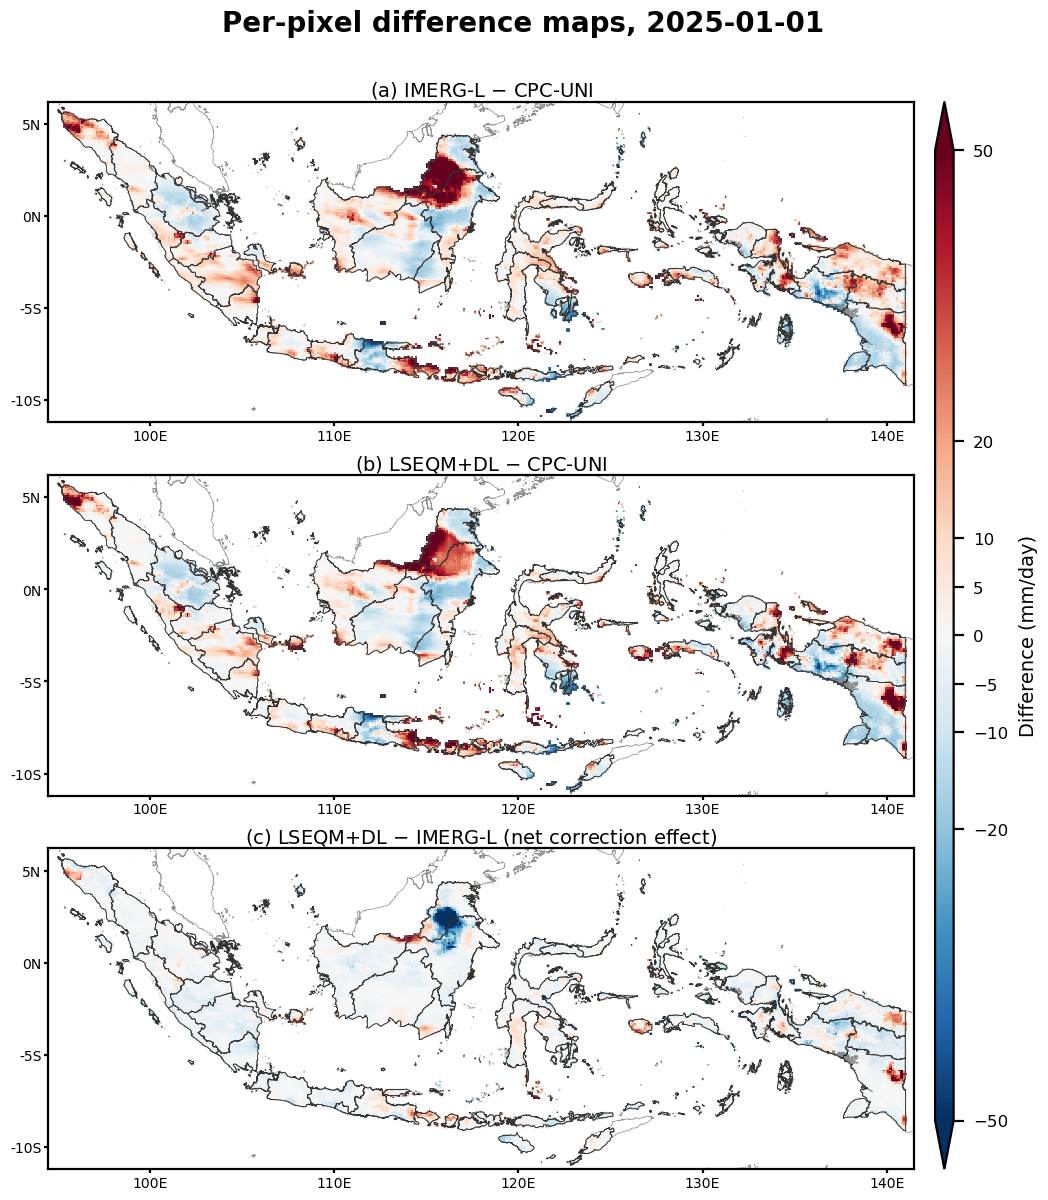
\includegraphics[width=\atlasGoneWidth\textwidth]{fig_thesis_G1_differences.png}
\caption[Difference maps locating the correction residual]{Difference maps for $1$~January~$2025$ (mm/day).\label{fig:atlas-diff}}
\end{figure}

Figure~\ref{fig:atlas-threedays} contrasts three days (the start,
middle, and end of dekad~$1$: $1$, $5$, and $10$~January) across IMERG-L
(raw), CPC-UNI (gauge reference), and LSEQM+DL (corrected); the
correction tracks the day-to-day variation of the gauge reference at all
three regimes without imposing a uniform overlay, preserving spatial
pattern while bringing the daily amount toward the gauge target.

\begin{figure}[H]
\centering
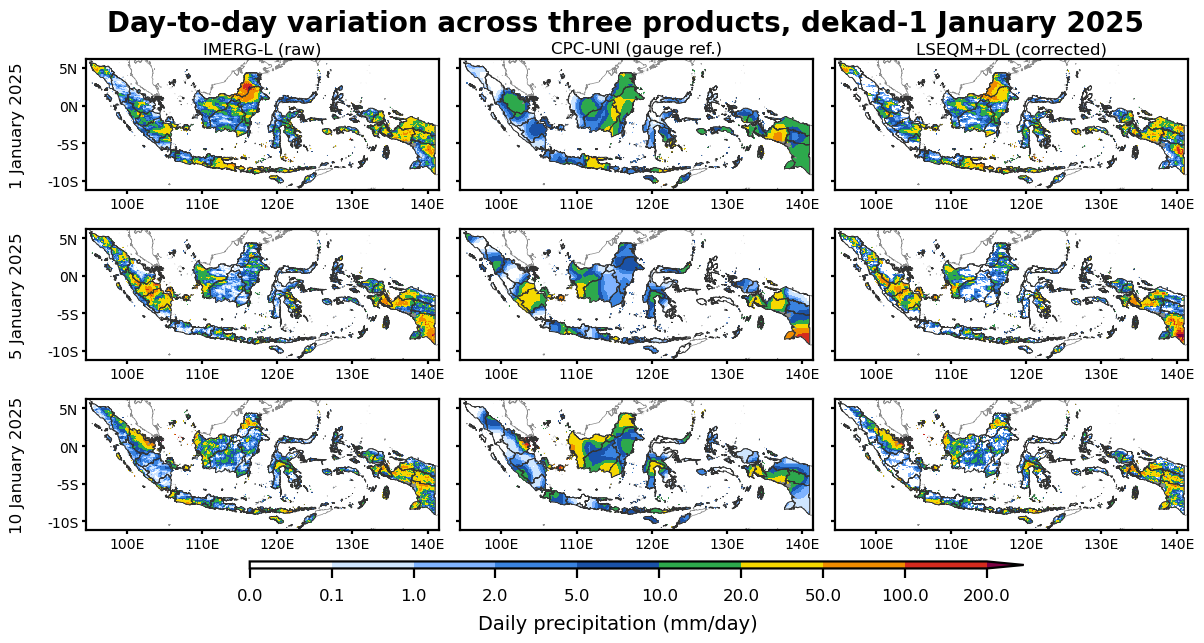
\includegraphics[width=\atlasGtwoWidth\textwidth]{fig_thesis_G2_three_days.png}
\caption[Three-day daily contrast across products]{Three-day daily contrast across products for dekad~$1$ of January~$2025$.\label{fig:atlas-threedays}}
\end{figure}

Figure~\ref{fig:atlas-pillars} maps the four verification pillars
(rows: relative bias, KS $p$-value, $Q_{99}$ ratio, and CSI) across the
LS, LSEQM, and LSEQM+DL stages (columns), computed over all
dekad-$1$-of-January samples in the $2001$ to $2025$ record; each row's
colour scale is set so that the pillar's target value (zero for bias,
unity otherwise) reads as neutral colour.

\begin{figure}[H]
\centering
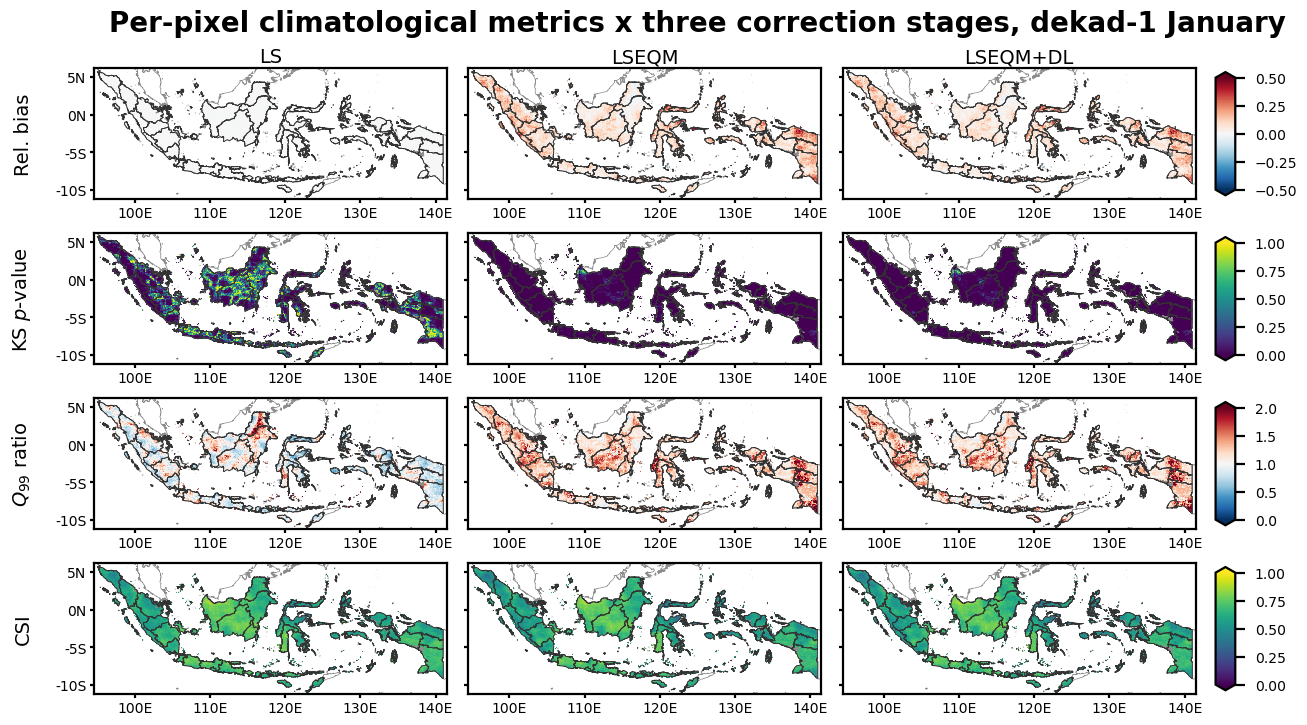
\includegraphics[width=\atlasGthreeWidth\textwidth]{fig_thesis_G3_pillar_metrics.png}
\caption[Per-pillar climatological metric maps across correction stages]{Per-pixel climatological metric maps for the four verification pillars across the three correction stages.\label{fig:atlas-pillars}}
\end{figure}

Figure~\ref{fig:atlas-six} maps six daily products on a shared colour
bar: the raw IMERG-L Late Run, the IMERG-F Final Run (the gauge-anchored
independent benchmark), the Linear Scaling stage, the LSEQM intermediate
(LS plus EQM plus GPD), the LSEQM+DL corrected output, and the CPC-UNI
gauge reference; reading the panels in sequence traces the correction
from raw retrieval to gauge reference.

\begin{figure}[H]
\centering
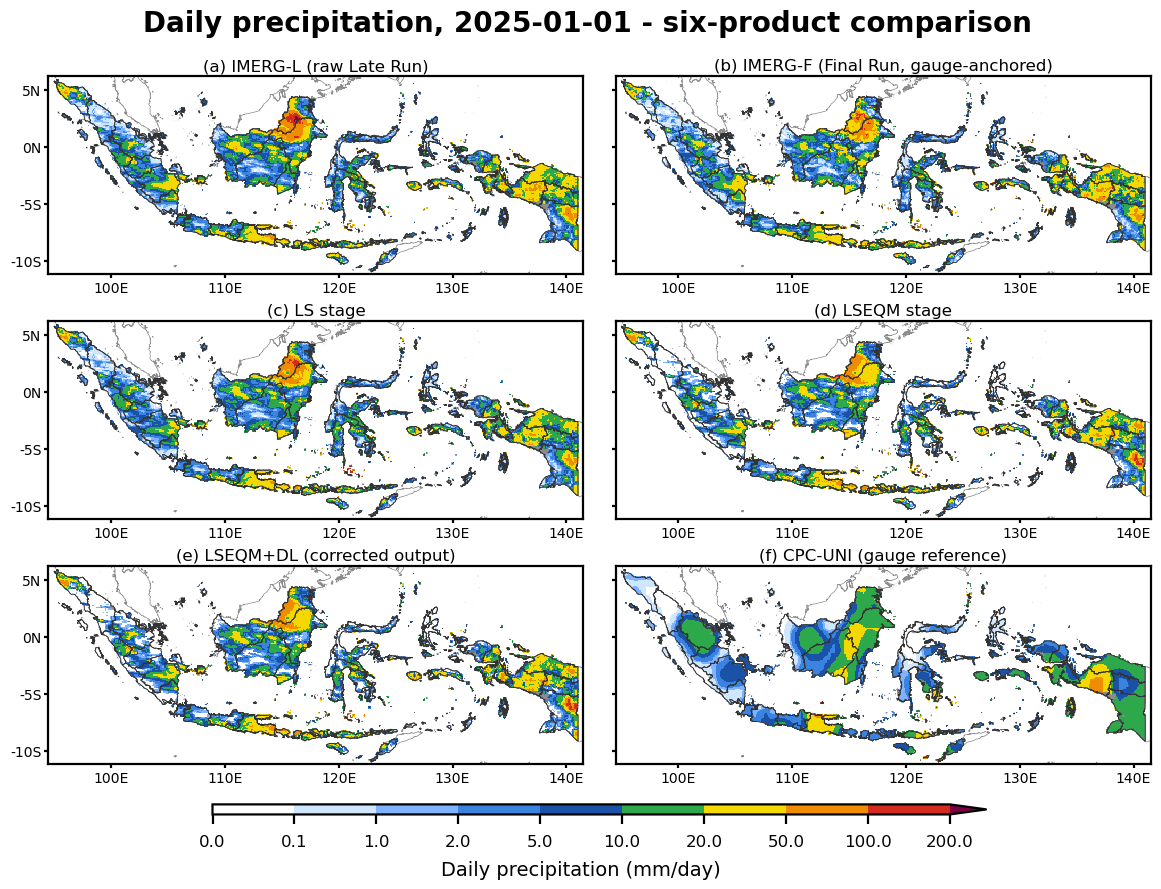
\includegraphics[width=\atlasGfourWidth\textwidth]{fig_thesis_G4_six_products.png}
\caption[Six-product comparison for 1 January 2025]{Six-product daily precipitation map for $1$~January~$2025$.\label{fig:atlas-six}}
\end{figure}

Figure~\ref{fig:atlas-stations} overlays the BMKG validation stations
(triangles coloured by their own dekad-$1$-of-January climatological
mean) on the same climatology for four products: CPC-UNI gauge analysis,
raw IMERG-L, corrected LSEQM+DL, and IMERG-F Final Run; where a
triangle's interior colour matches the surrounding gridded colour, the
gridded product agrees with the station.

\begin{figure}[H]
\centering
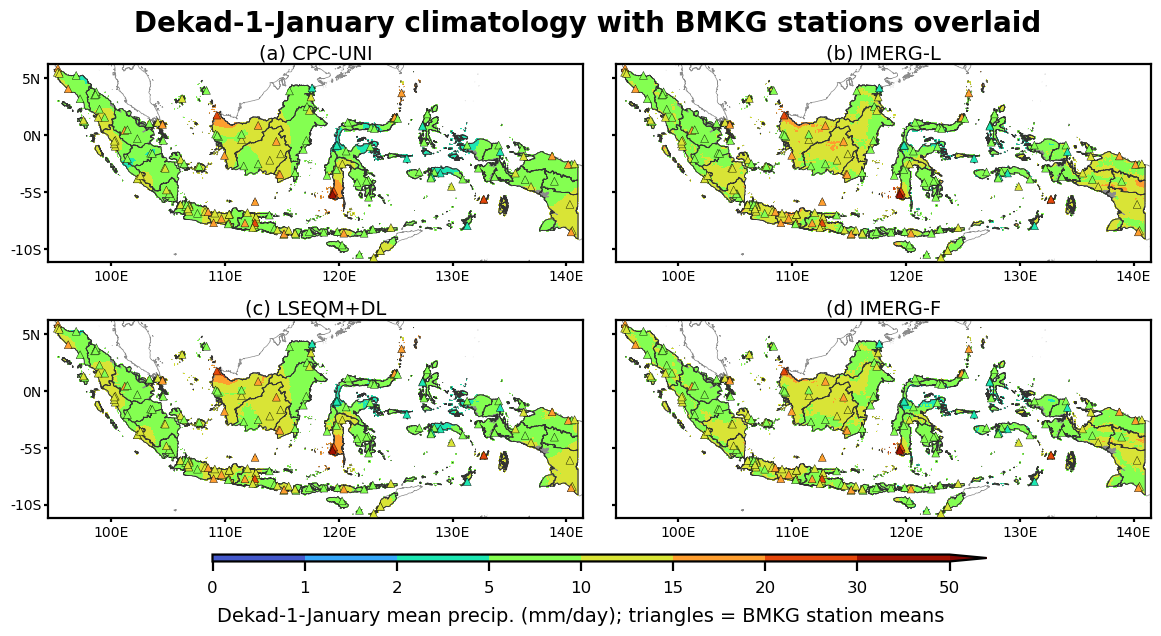
\includegraphics[width=\atlasGfiveWidth\textwidth]{fig_thesis_G5_station_overlay.png}
\caption[Station-overlay maps for dekad-1-January climatology]{Dekad-$1$-of-January climatological mean precipitation (mm/day, $2001$ to $2025$ average) for four products with the BMKG validation stations overlaid.\label{fig:atlas-stations}}
\end{figure}


% ============================================================
\chapter{Supplementary Temporal-Alignment Diagnostics}\label{app:window}
\addcontentsline{apx}{appx}{\protect\numberline{Appendix~\thechapter}Supplementary Temporal-Alignment Diagnostics}
% ============================================================

% --- Tunable per-figure widths (fraction of \textwidth) ---
\newcommand{\gridTrmmWidth}{1.0}   % H.1 gridded-CPC, TRMM-input era (full text width)
\newcommand{\gridGpmWidth}{1.0}    % H.2 gridded-CPC, GPM era (full text width)

The whole-domain window-offset diagnostic of
Section~\ref{sec:discussion-subdaily} (Figure~\ref{fig:gridded-cpc})
is shown here separately for the two satellite eras, with the
per-timezone-band pooled correlation the main-text figure omits.

\begin{figure}[H]
\centering
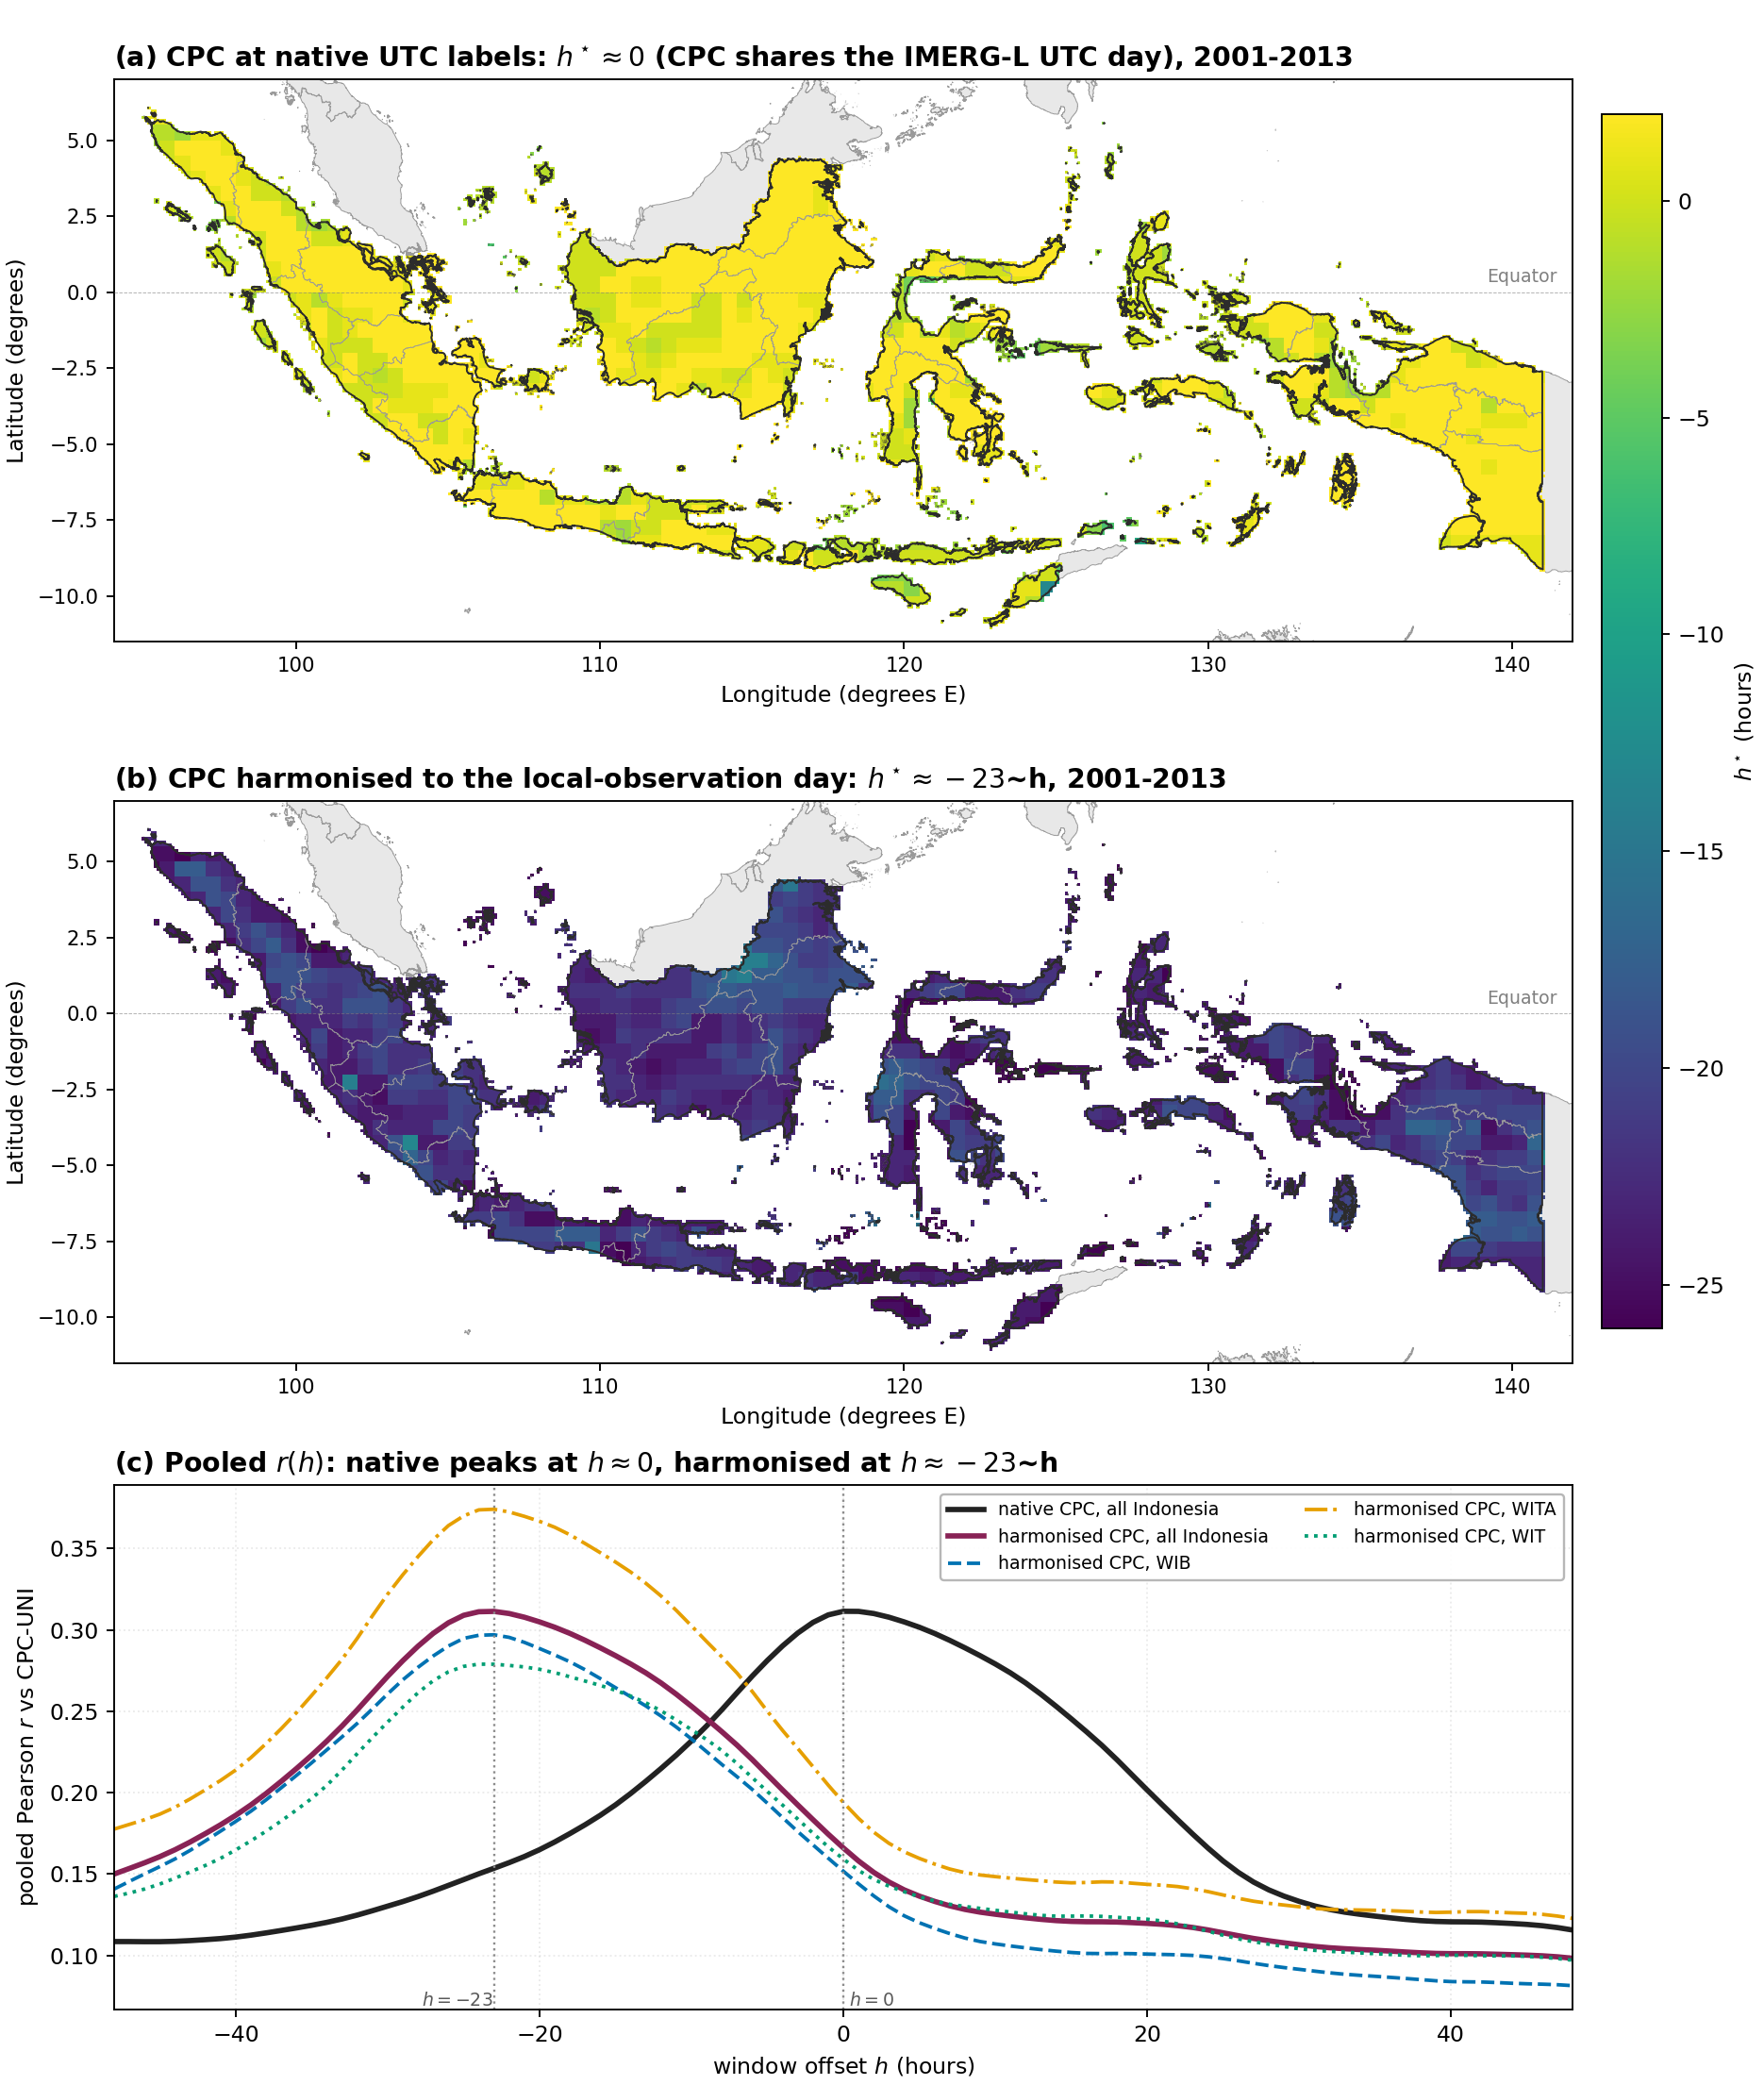
\includegraphics[width=\gridTrmmWidth\textwidth]{fig_thesis_H1_gridded_trmm.png}
\caption[Gridded window offset against CPC-UNI, TRMM-input era]{Gridded
window-offset diagnostic against CPC-UNI over the TRMM-input era ($2001$ to
$2013$).\label{fig:grid-trmm}}
\end{figure}

Each figure maps the optimal aggregation-window offset $h^\star$
of the half-hourly IMERG-L source against the gridded CPC-UNI
analysis at every $0.5^\circ$ cell, at CPC-UNI's native UTC labels
(panel a, $h^\star\approx0$) and after harmonising CPC-UNI to the
local-observation day (panel b, $h^\star\approx-23$~h), with the
pooled $r(h)$ and its per-band decomposition below (panel c). The
native optimum sits at $h^\star\approx0$ across the
gauge-constrained western and central cells in both eras, the
whole-domain signature of CPC-UNI sharing the IMERG-L UTC calendar
date; the data-sparse eastern cells, where the CPC-UNI gauge
network thins, carry low and noisy $h^\star$ and are read together
with CPC gauge density.

\begin{figure}[H]
\centering
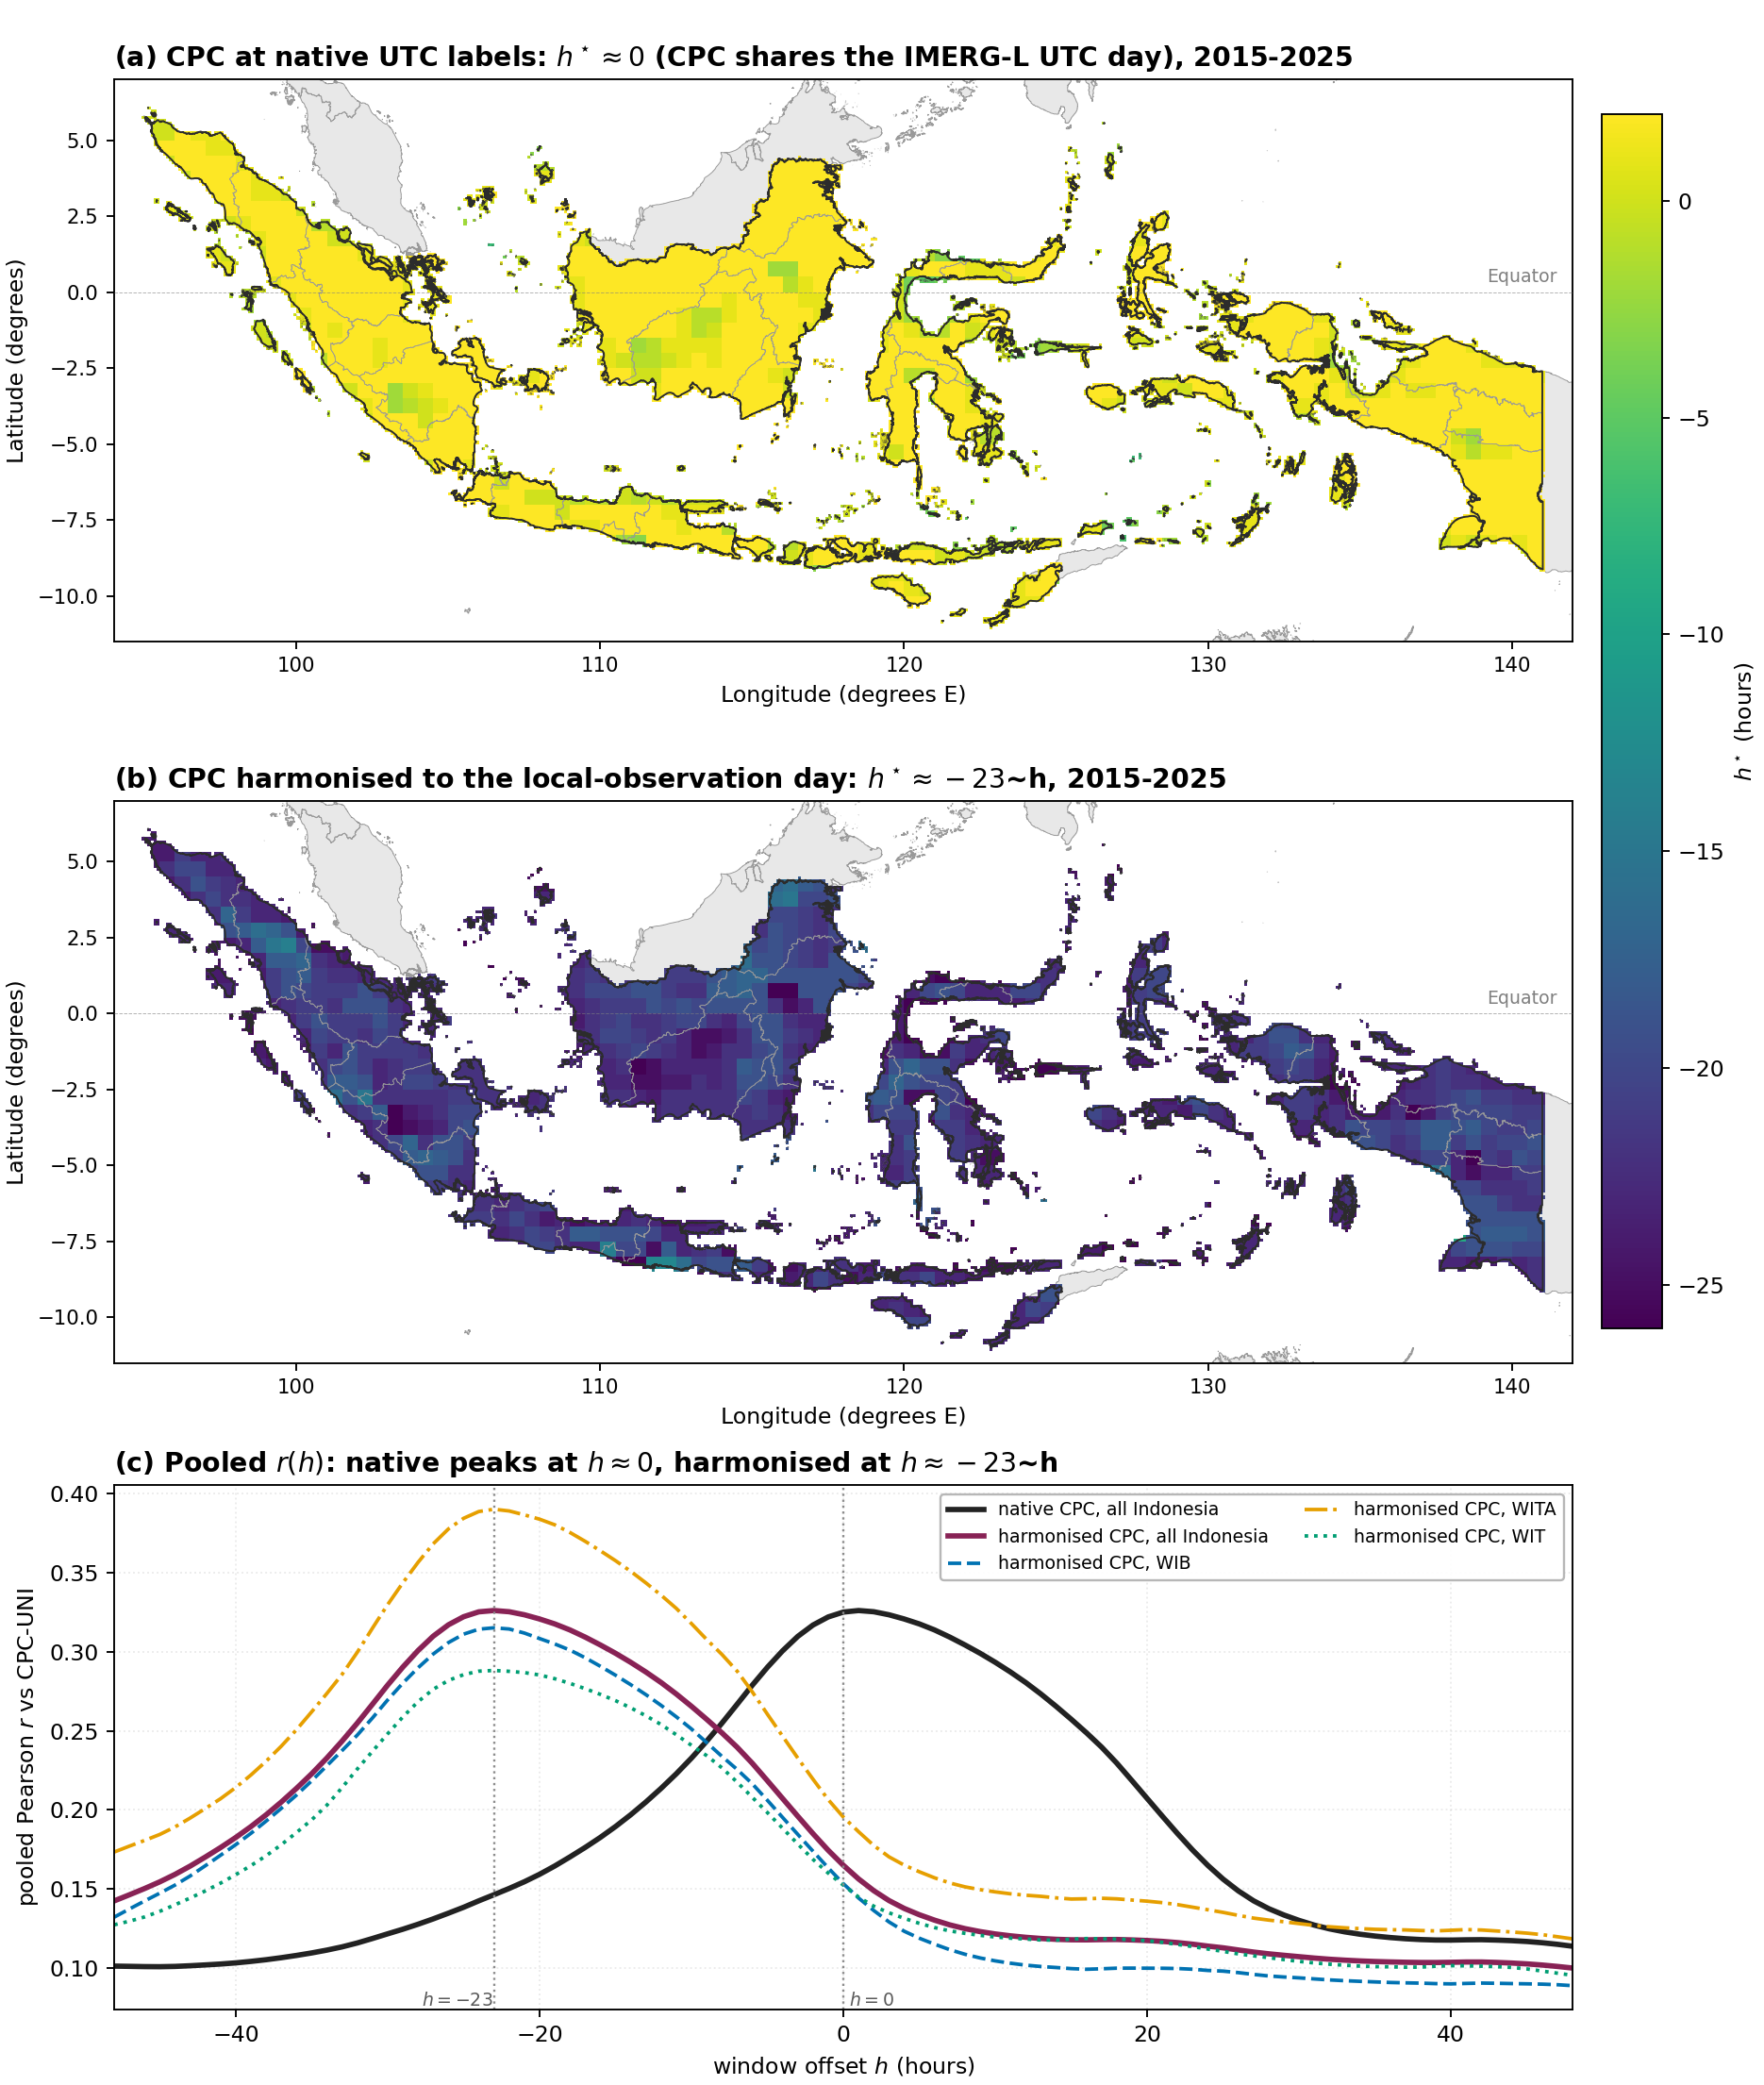
\includegraphics[width=\gridGpmWidth\textwidth]{fig_thesis_H2_gridded_gpm.png}
\caption[Gridded window offset against CPC-UNI, GPM era]{Gridded window-offset
diagnostic against CPC-UNI over the GPM era ($2015$ to
$2025$).\label{fig:grid-gpm}}
\end{figure}

The optimum is the same in the timing-imprecise TRMM-input era
(Figure~\ref{fig:grid-trmm}) as in the GPM era
(Figure~\ref{fig:grid-gpm}), confirming that the offset is a
property of the gauge-labelling convention rather than of the
satellite retrieval skill. The absolute correlation against the
smoothed $0.5^\circ$ analysis is muted in both eras and so does
not reproduce the point-gauge era recovery documented in
Section~\ref{sec:results-window}, while the spatial coverage that
the gridded reference adds, beyond the BMKG station locations,
shows the offset to be uniform across the gauge-constrained part
of the archipelago.


% Restore the body chapter heading style, which chapter_99_appendices.tex
% replaces with the appendix look. Anything included after the appendices needs
% this. Keep in sync with the \titleformat/\titlespacing block in the preamble.
\titleformat{\chapter}[hang]
  {\global\leftskip=0pt\global\InHthreefalse\normalfont\fontsize{14}{17}\bfseries\filcenter}
  {\thechapter}{1ex}{\MakeUppercase}
\titlespacing*{\chapter}{0pt}{0pt}{2\baselineskip}

% --- Biography (last page) ---
\cleardoublepage
% ============================================================
% biography.tex - CURRICULUM VITAE, the final page after the appendices.
%
% Content follows PPKI 3.3.2 and Appendix 14b: birth, education, career, and a
% publication-history sentence naming the journal that carried the companion
% paper. Set as \chapter* so the title takes the standard chapter treatment.
% main_thesis.tex issues the page break before \input.
% Included by main_thesis.tex.
% License: CC BY 4.0 (see ../LICENSE).
% ============================================================
\pdfbookmark[0]{CURRICULUM VITAE}{cv-bookmark}
\chapter*{Curriculum Vitae}\thispagestyle{fancy}

The author was born in Tuban, East Java, in 1982. He earned his undergraduate degree 
in Meteorology from Bogor Agricultural University in 2006. Over the past 15 years, he 
has worked extensively in climate analytics and geospatial technology for international 
organizations, including a decade with the United Nations and five years with the World Bank Group. 
In 2022, he began his graduate studies in Applied Climatology at Bogor Agricultural University.

The scientific paper entitled ``A Modular and Transferable
Framework for Enhancing Satellite-Derived Daily Precipitation: Adjusting Values, Aligning
Distributions, and Preserving Extremes'' was published in \emph{Remote Sensing}
18(14):2298 (doi:10.3390/rs18142298), co-authored with both supervisors. This scientific
paper was part of the author's master's program.

\end{document}
